%\section{3D-modeled Facade Variations across Patterns}
%\label{sec:AnnexVariations}
%%\section{3D-modeled Facade Variations across Patterns}
%\label{sec:AnnexVariations}
%%\section{3D-modeled Facade Variations across Patterns}
%\label{sec:AnnexVariations}
%%\section{3D-modeled Facade Variations across Patterns}
%\label{sec:AnnexVariations}
%\input{Text/AnnexVariations}

Facade Variations generated for each of the 3 patterns created in Blender and projected during the VR experiment, illustrated in Tables \ref{tab:PatternsVariationsPart1} and \ref{tab:PatternsVariationsPart2}.

    %%Table: Pattern Variations 1 to 5. Part1
    \begin{table*}[htb]
        \centering
        \small
        \caption{Patterns variations for the First five levels of complexity}
        \label{tab:PatternsVariationsPart1}
        \begin{tabularx}
        {\textwidth}{p{3cm} >{\centering\arraybackslash}X >{\centering\arraybackslash}X >{\centering\arraybackslash}X }
            \toprule
            \textit{Description} &
              \textit{Pattern 1} &
              \textit{Pattern 2} &
              \textit{Pattern 3} \\
            \midrule
            \text{Pattern Name} & Hishi Pattern & Tortoise shells & Asanoha Pattern\\

            \midrule
            \textit{Base Module} &  &  &
            \\
            {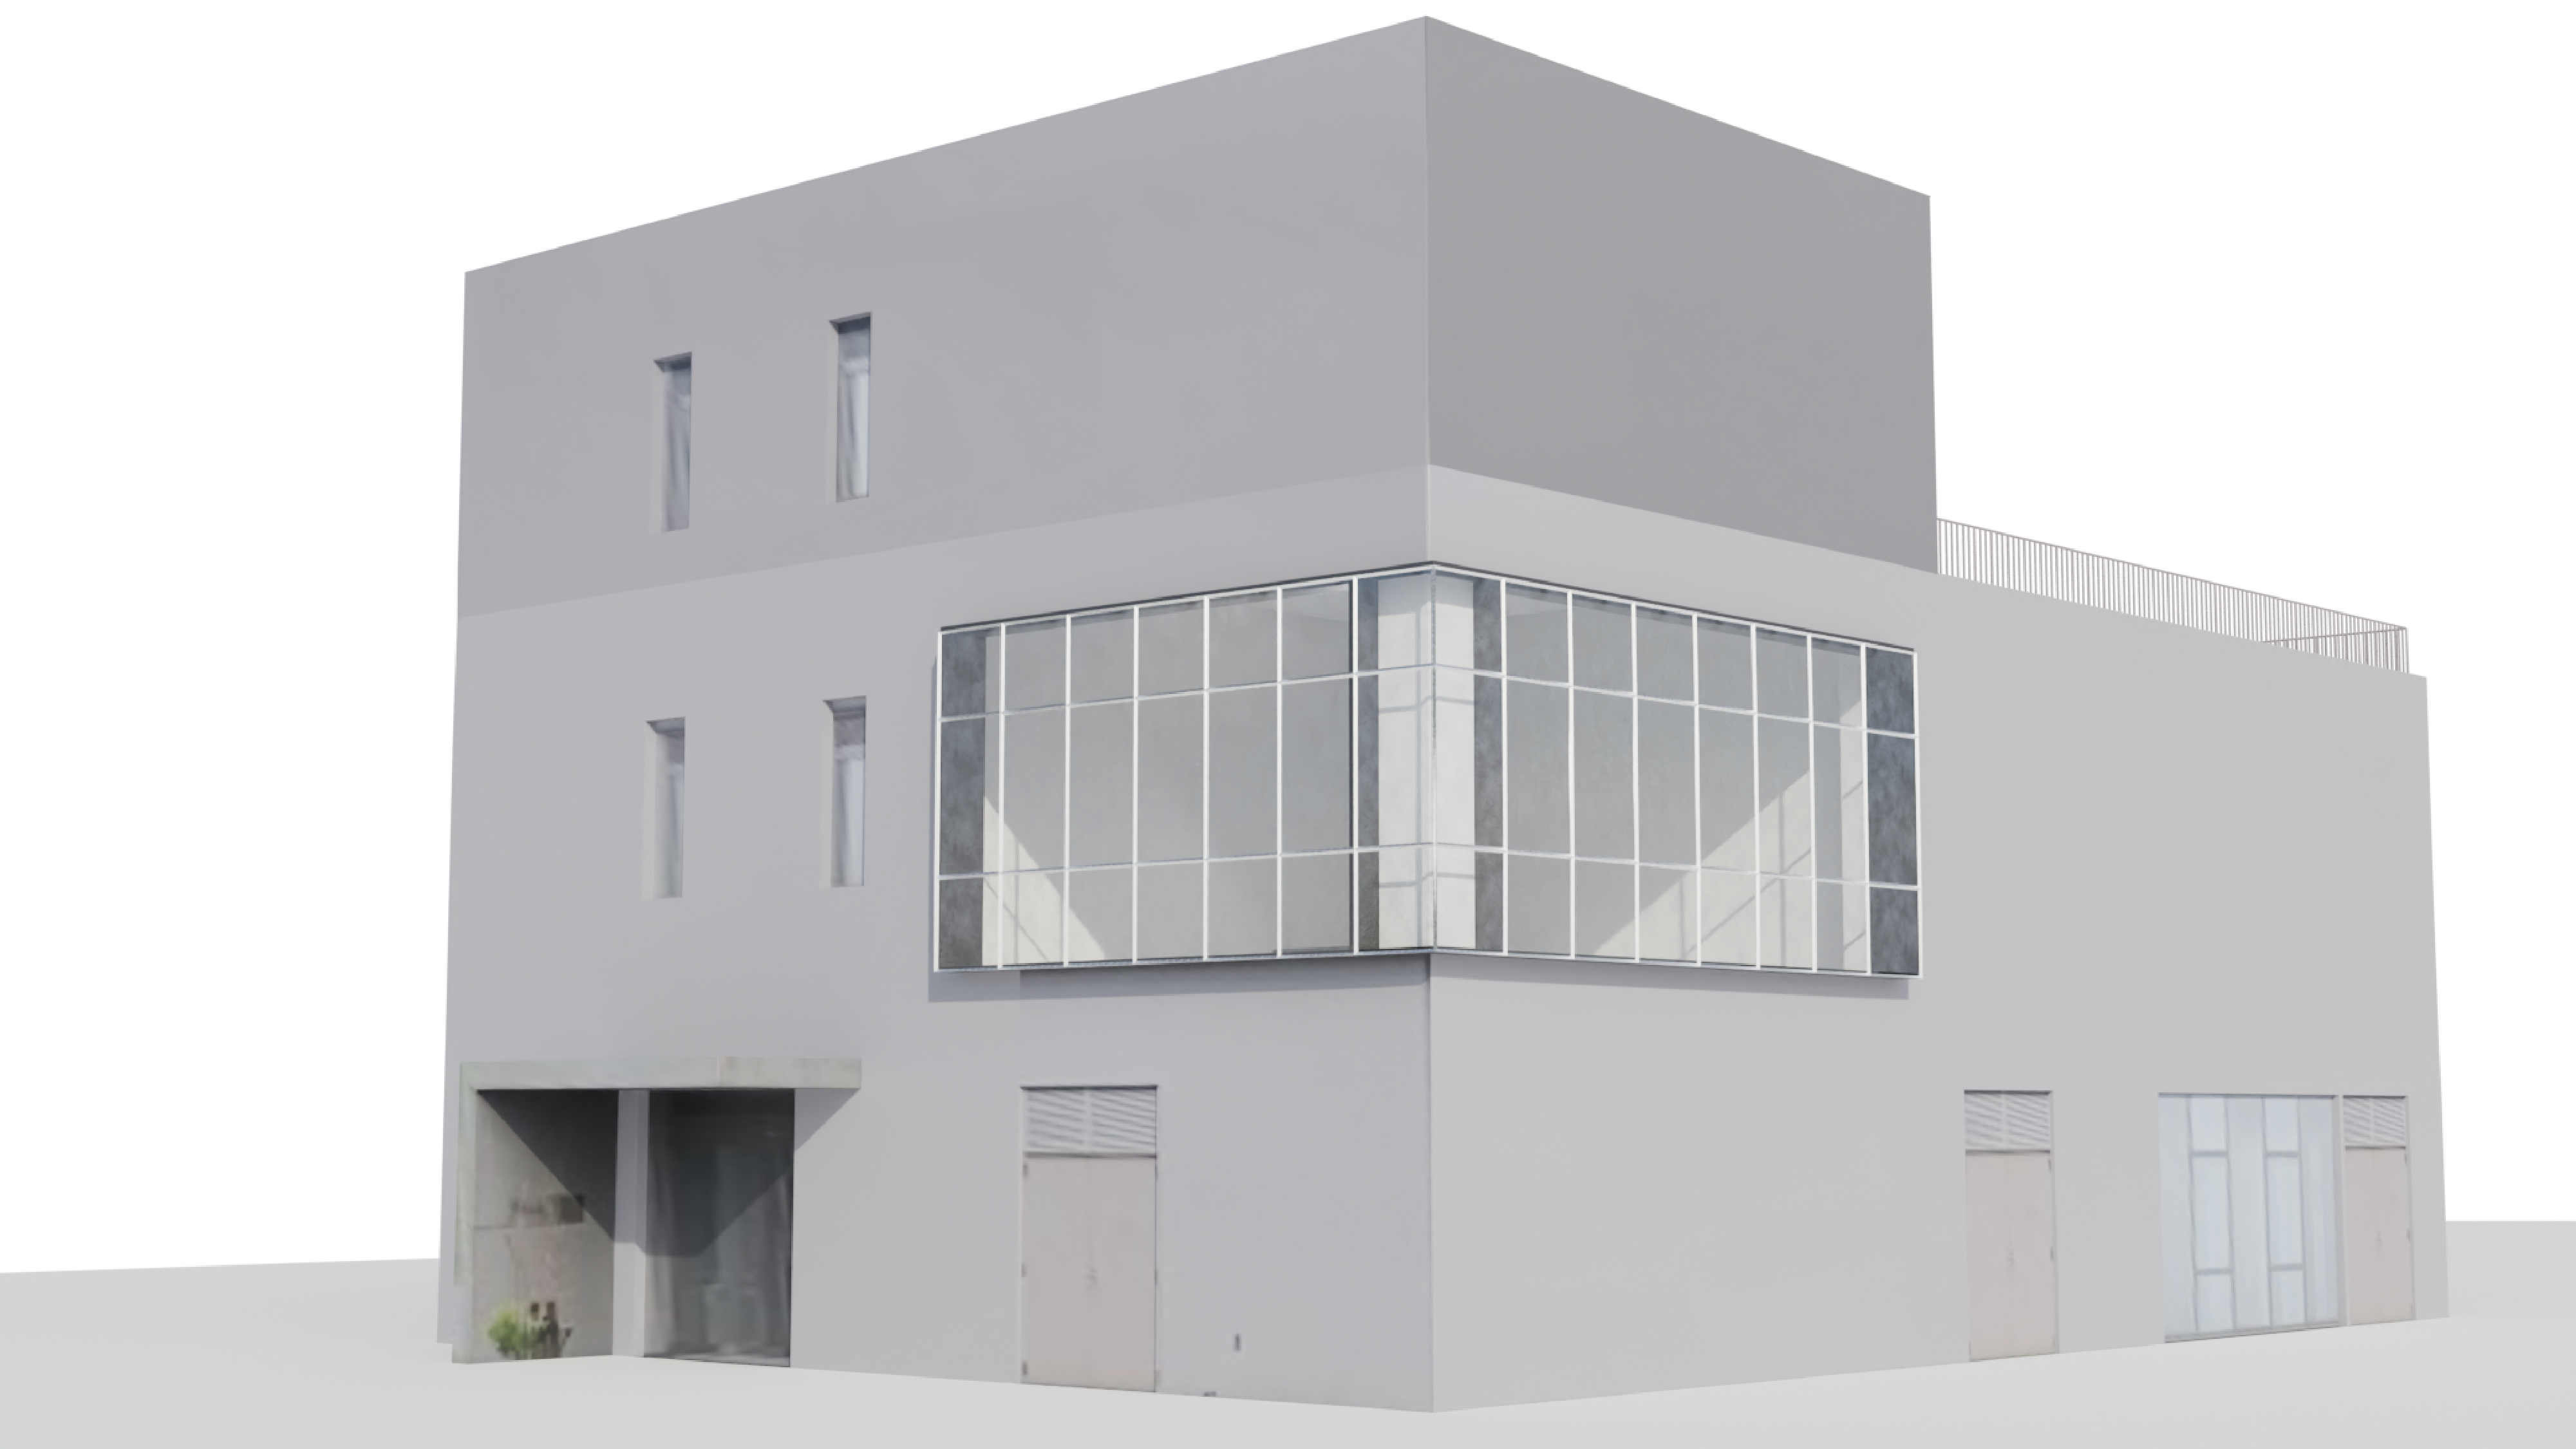
\includegraphics[width=1\linewidth]{Images/Base Module/Building}} &
              {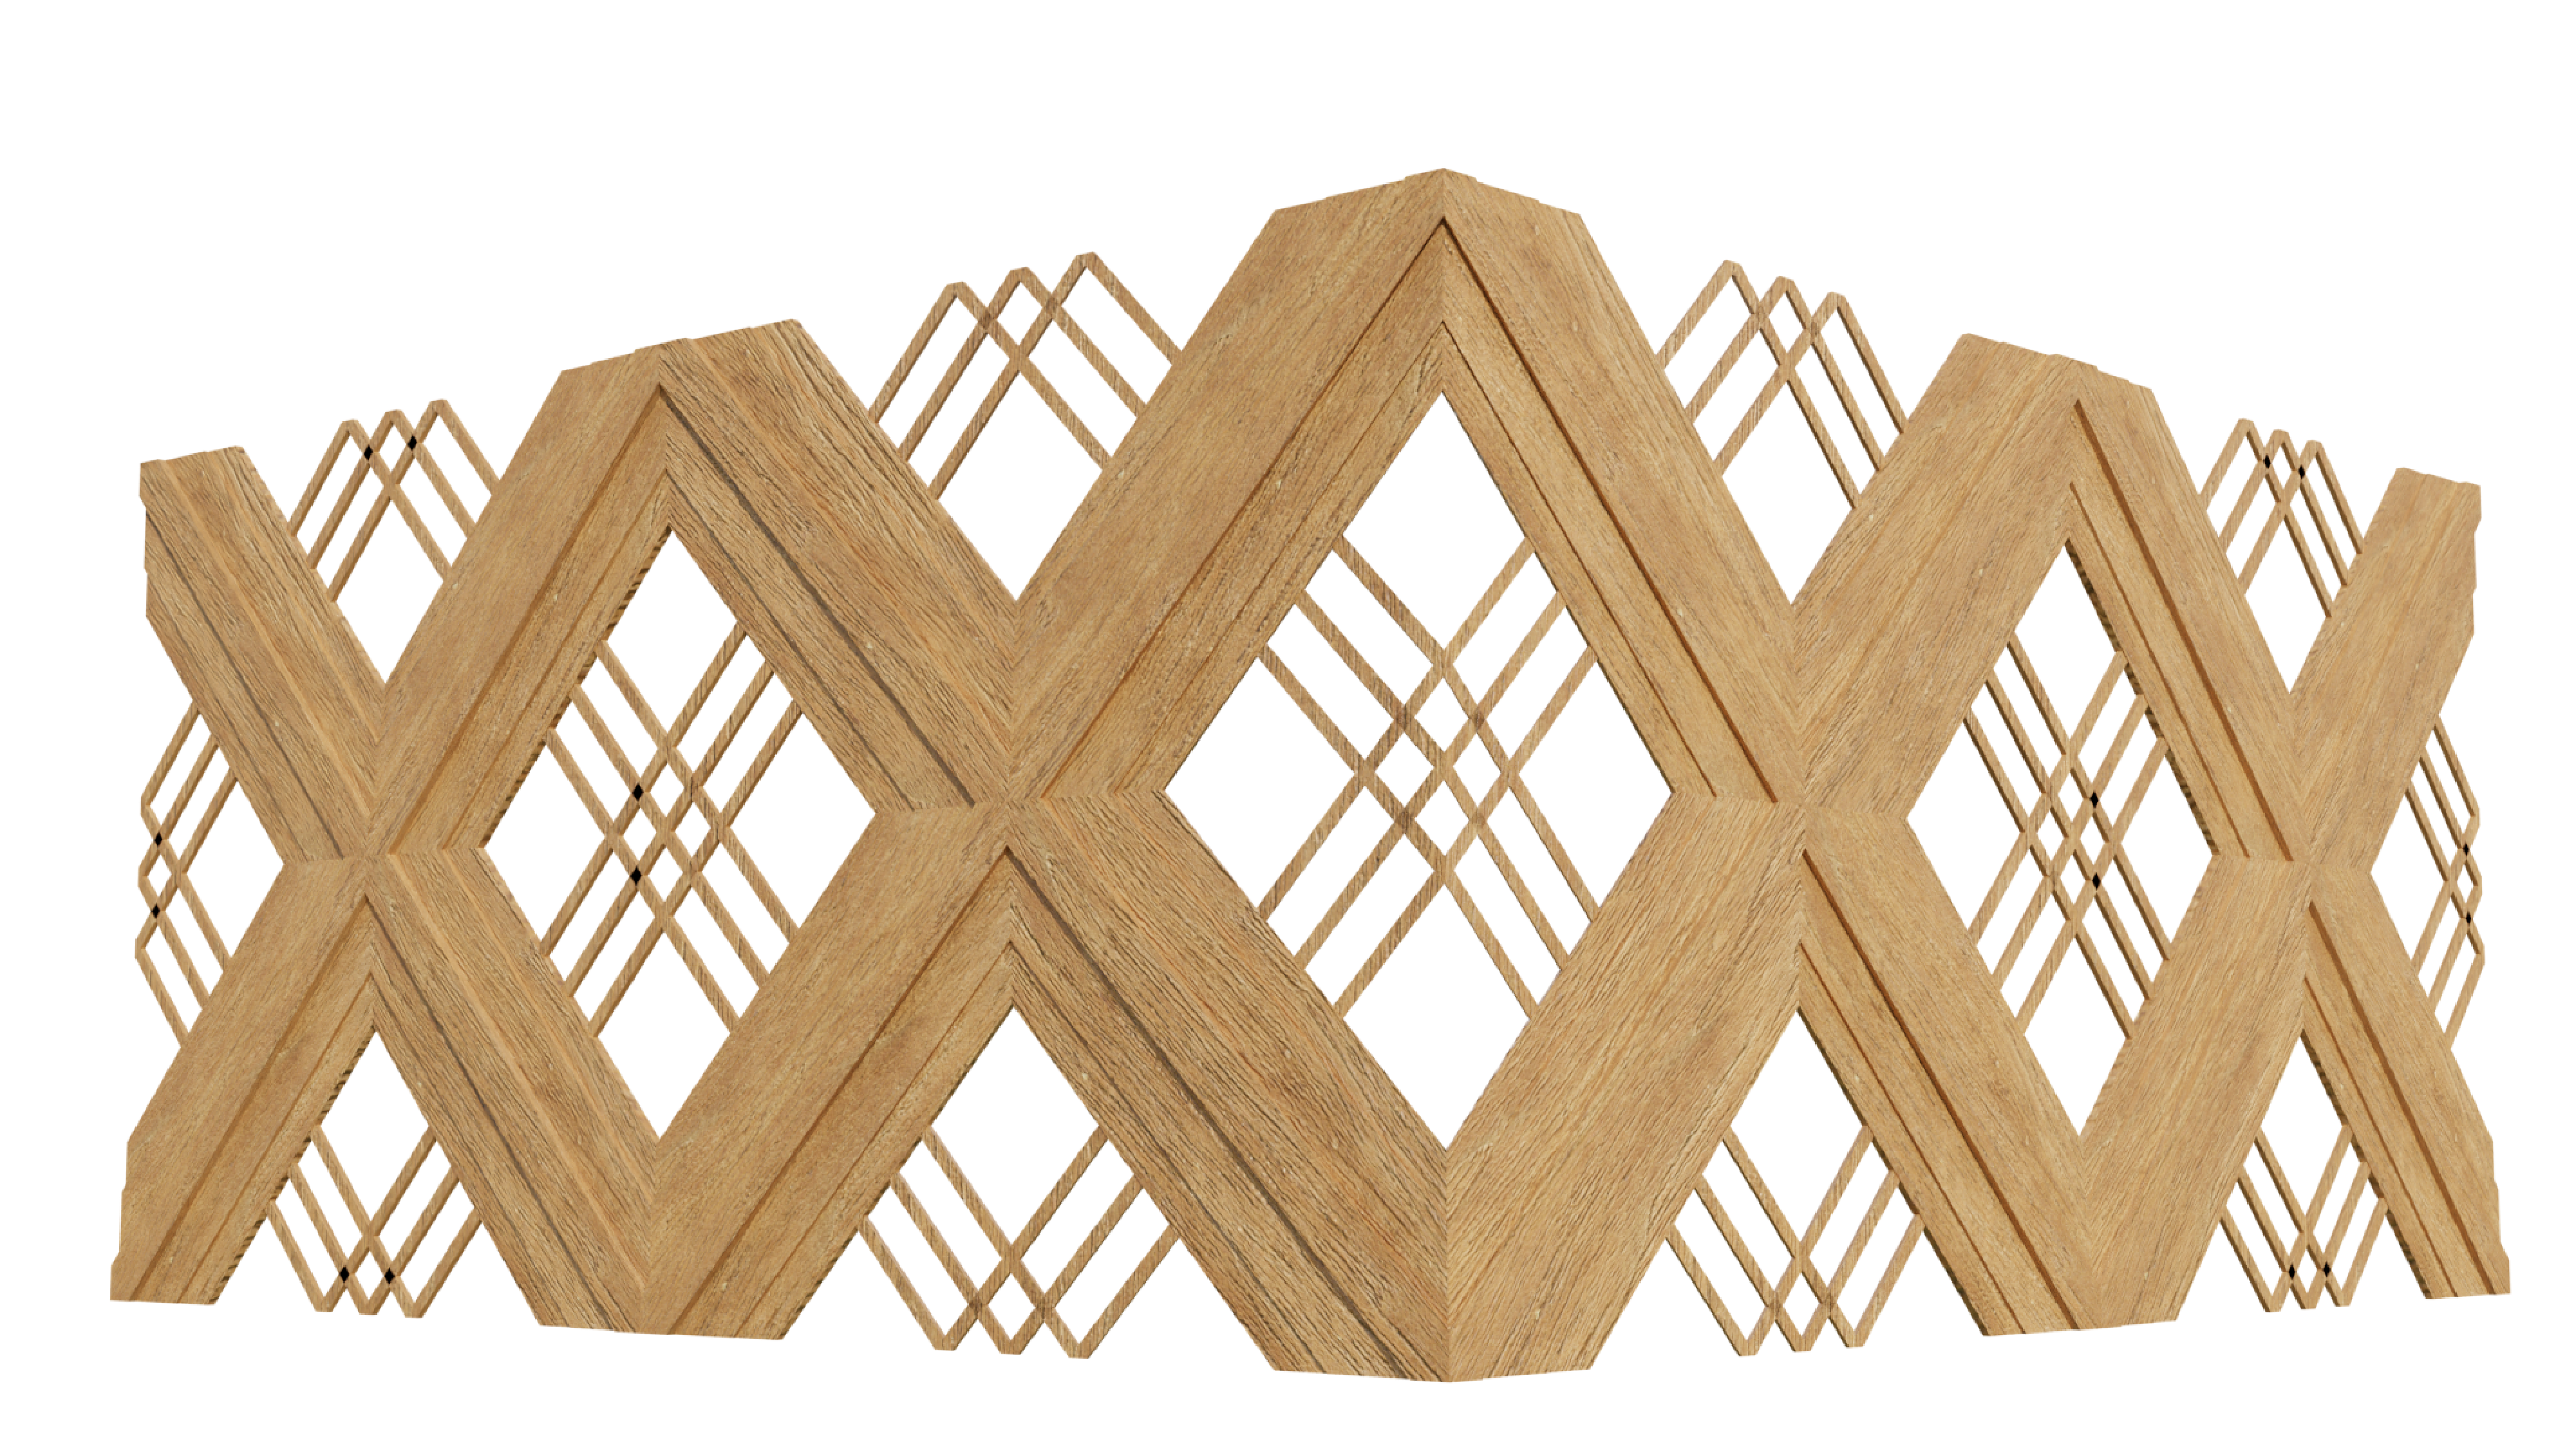
\includegraphics[width=1\linewidth]{Images/Base Module/Pattern1}} &
              {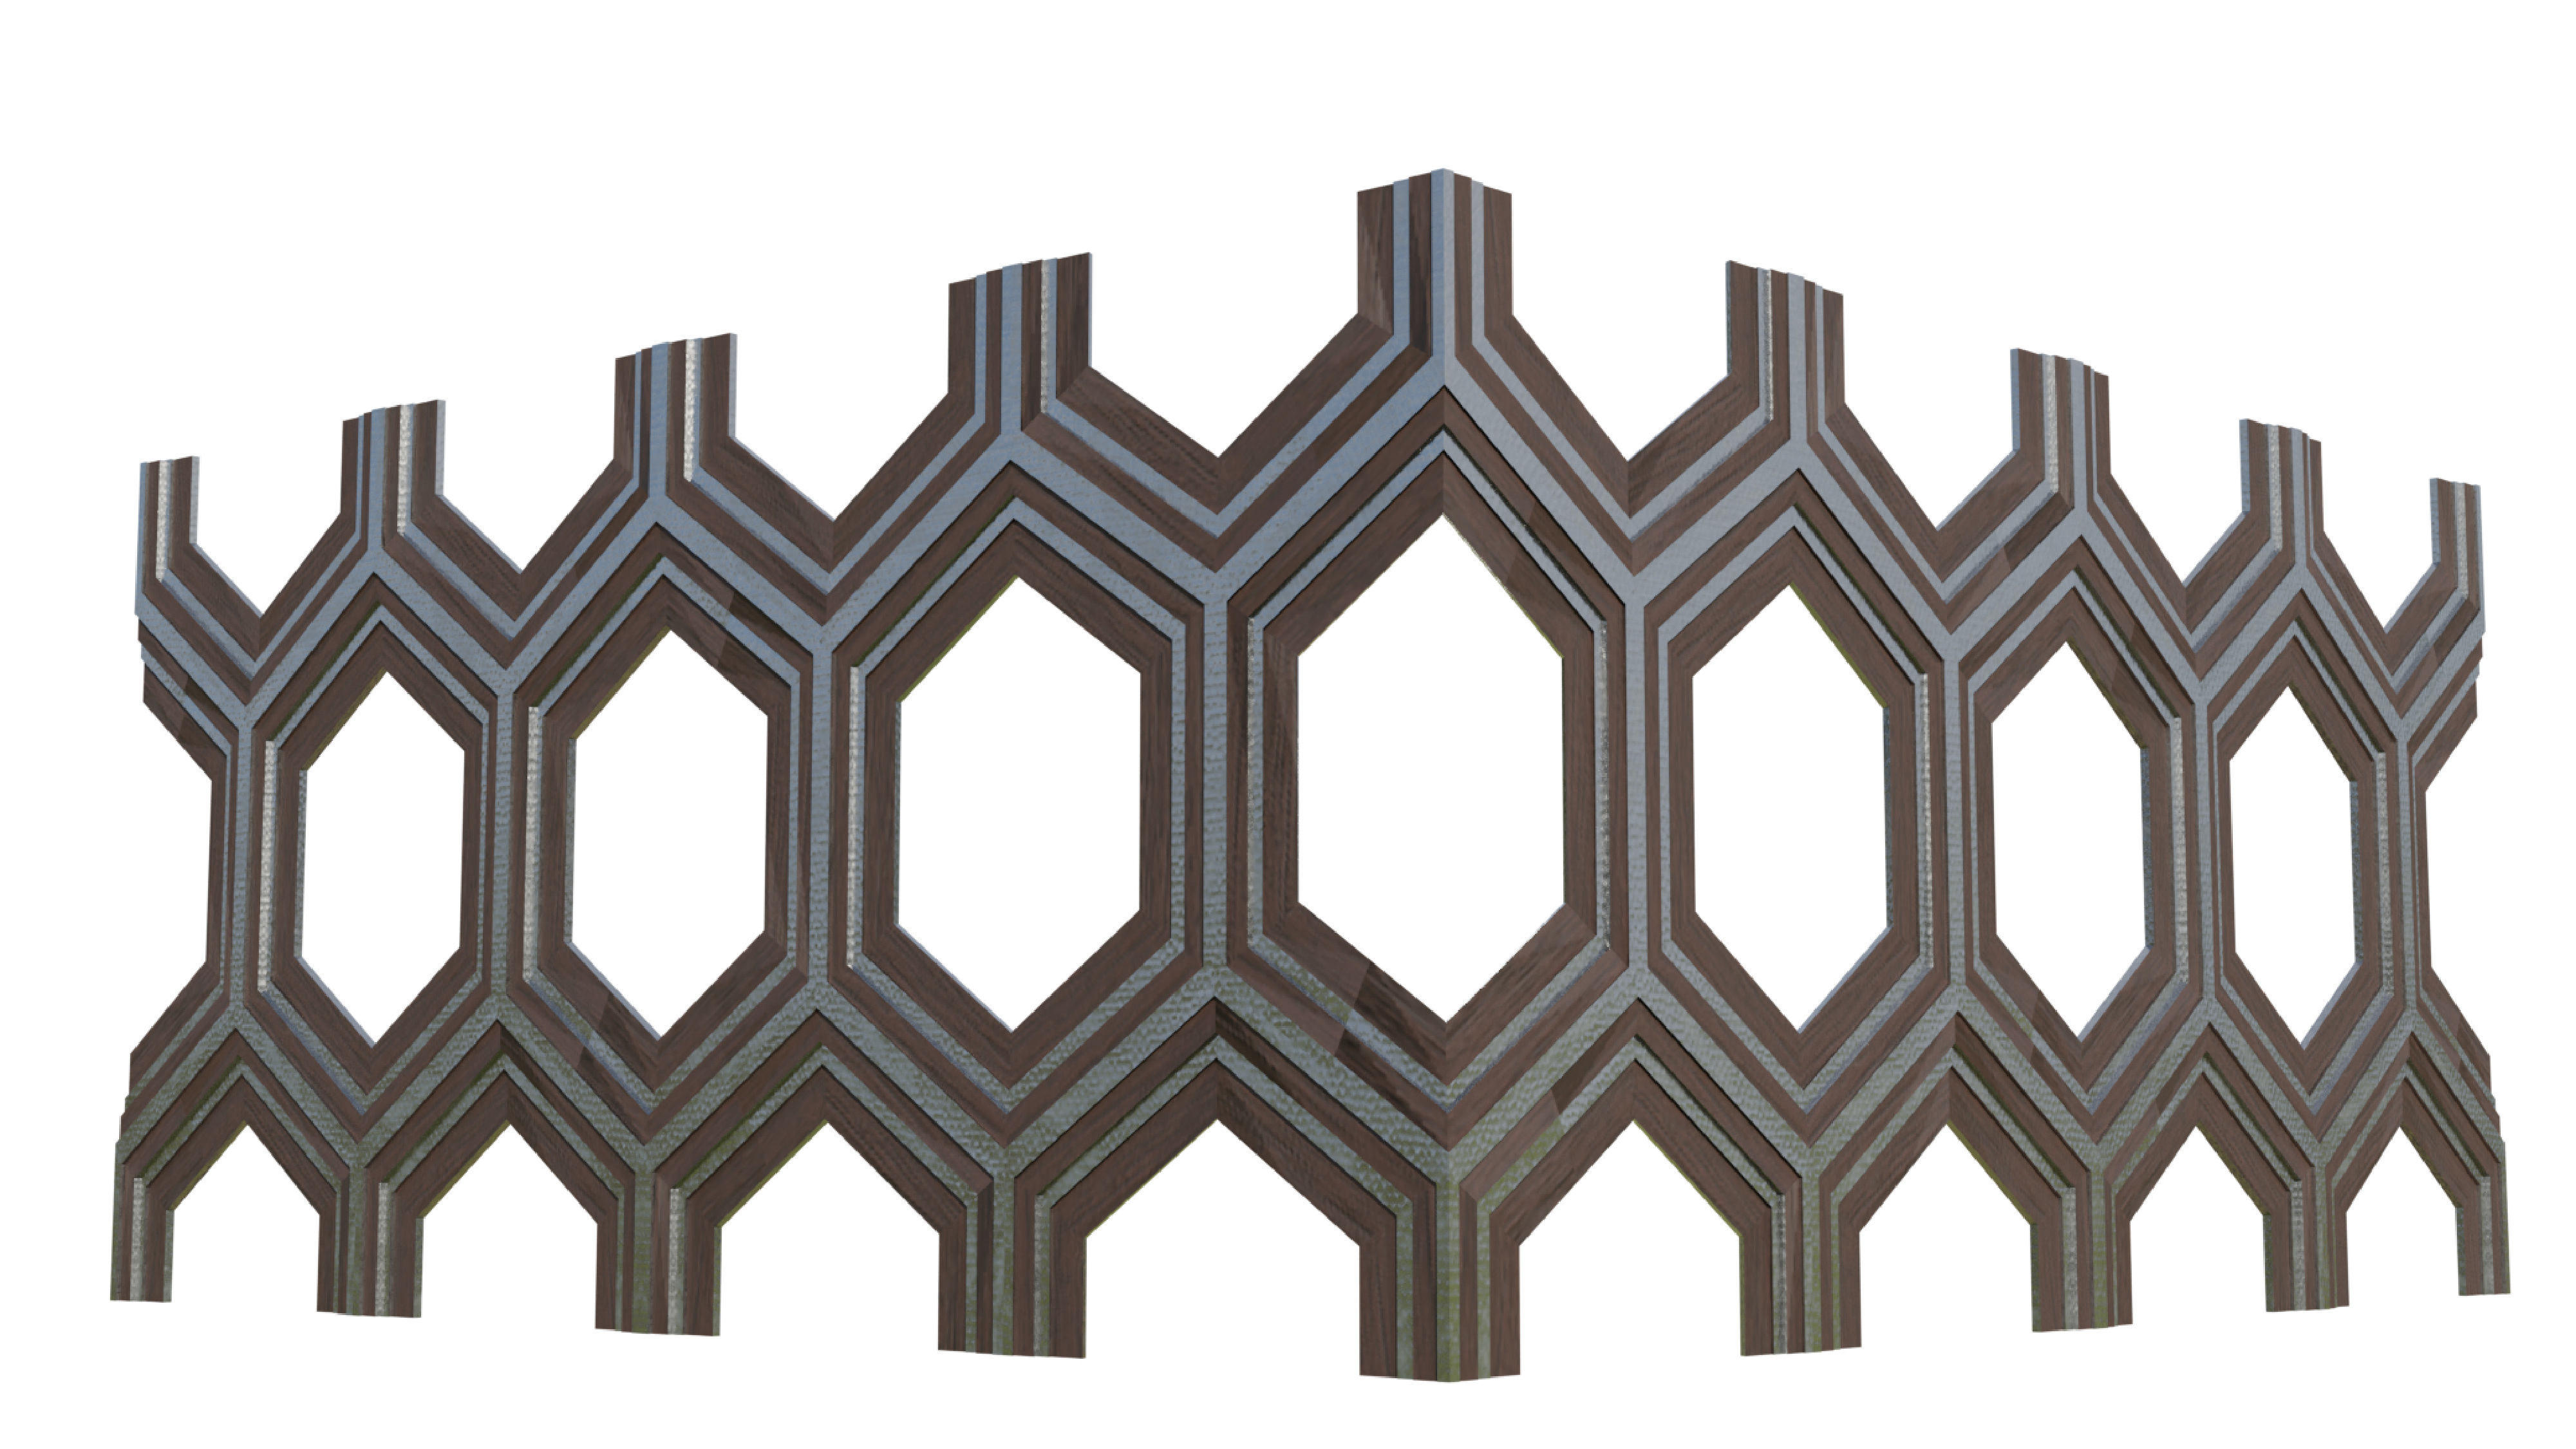
\includegraphics[width=1\linewidth]{Images/Base Module/Pattern2}} &
              {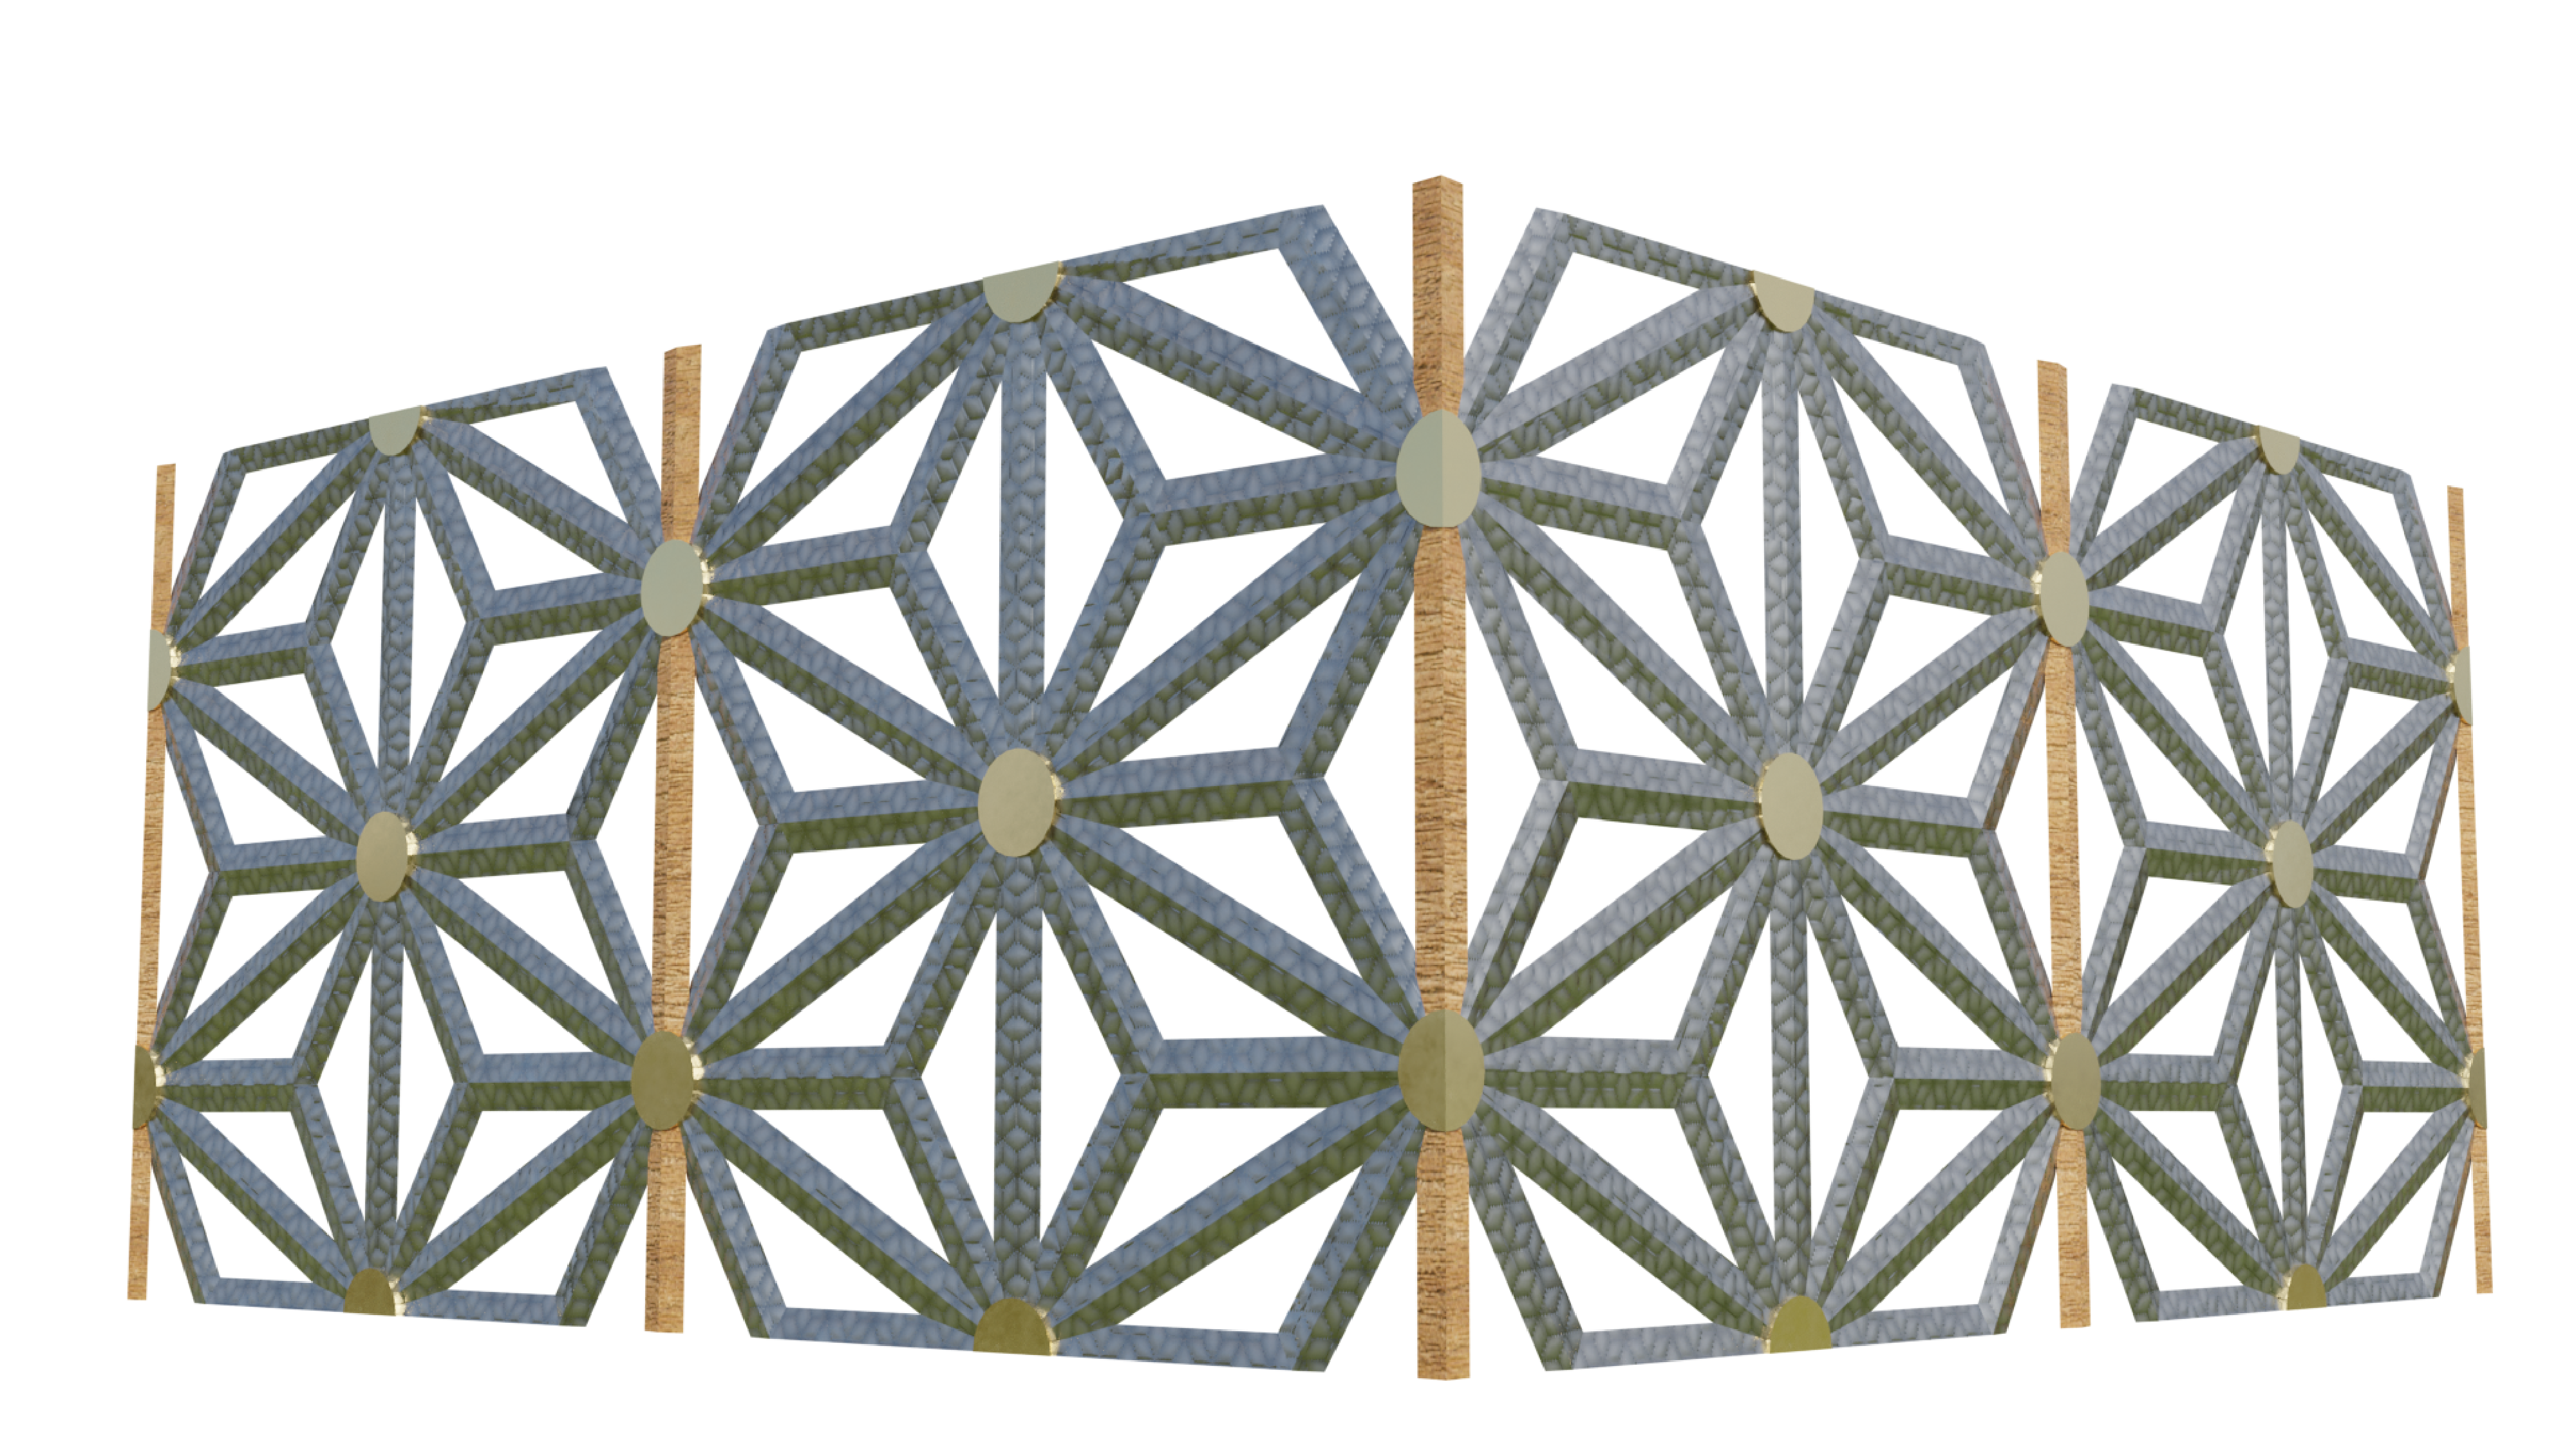
\includegraphics[width=1\linewidth]{Images/Base Module/Pattern3}} \\
            \midrule

            \textit{Mesh complexity Level} &
              \textit{Pattern 1} &
              \textit{Pattern 2} &
              \textit{Pattern 3}\\

            \midrule
            \textit{Level 1} &  &  &
            \\
            {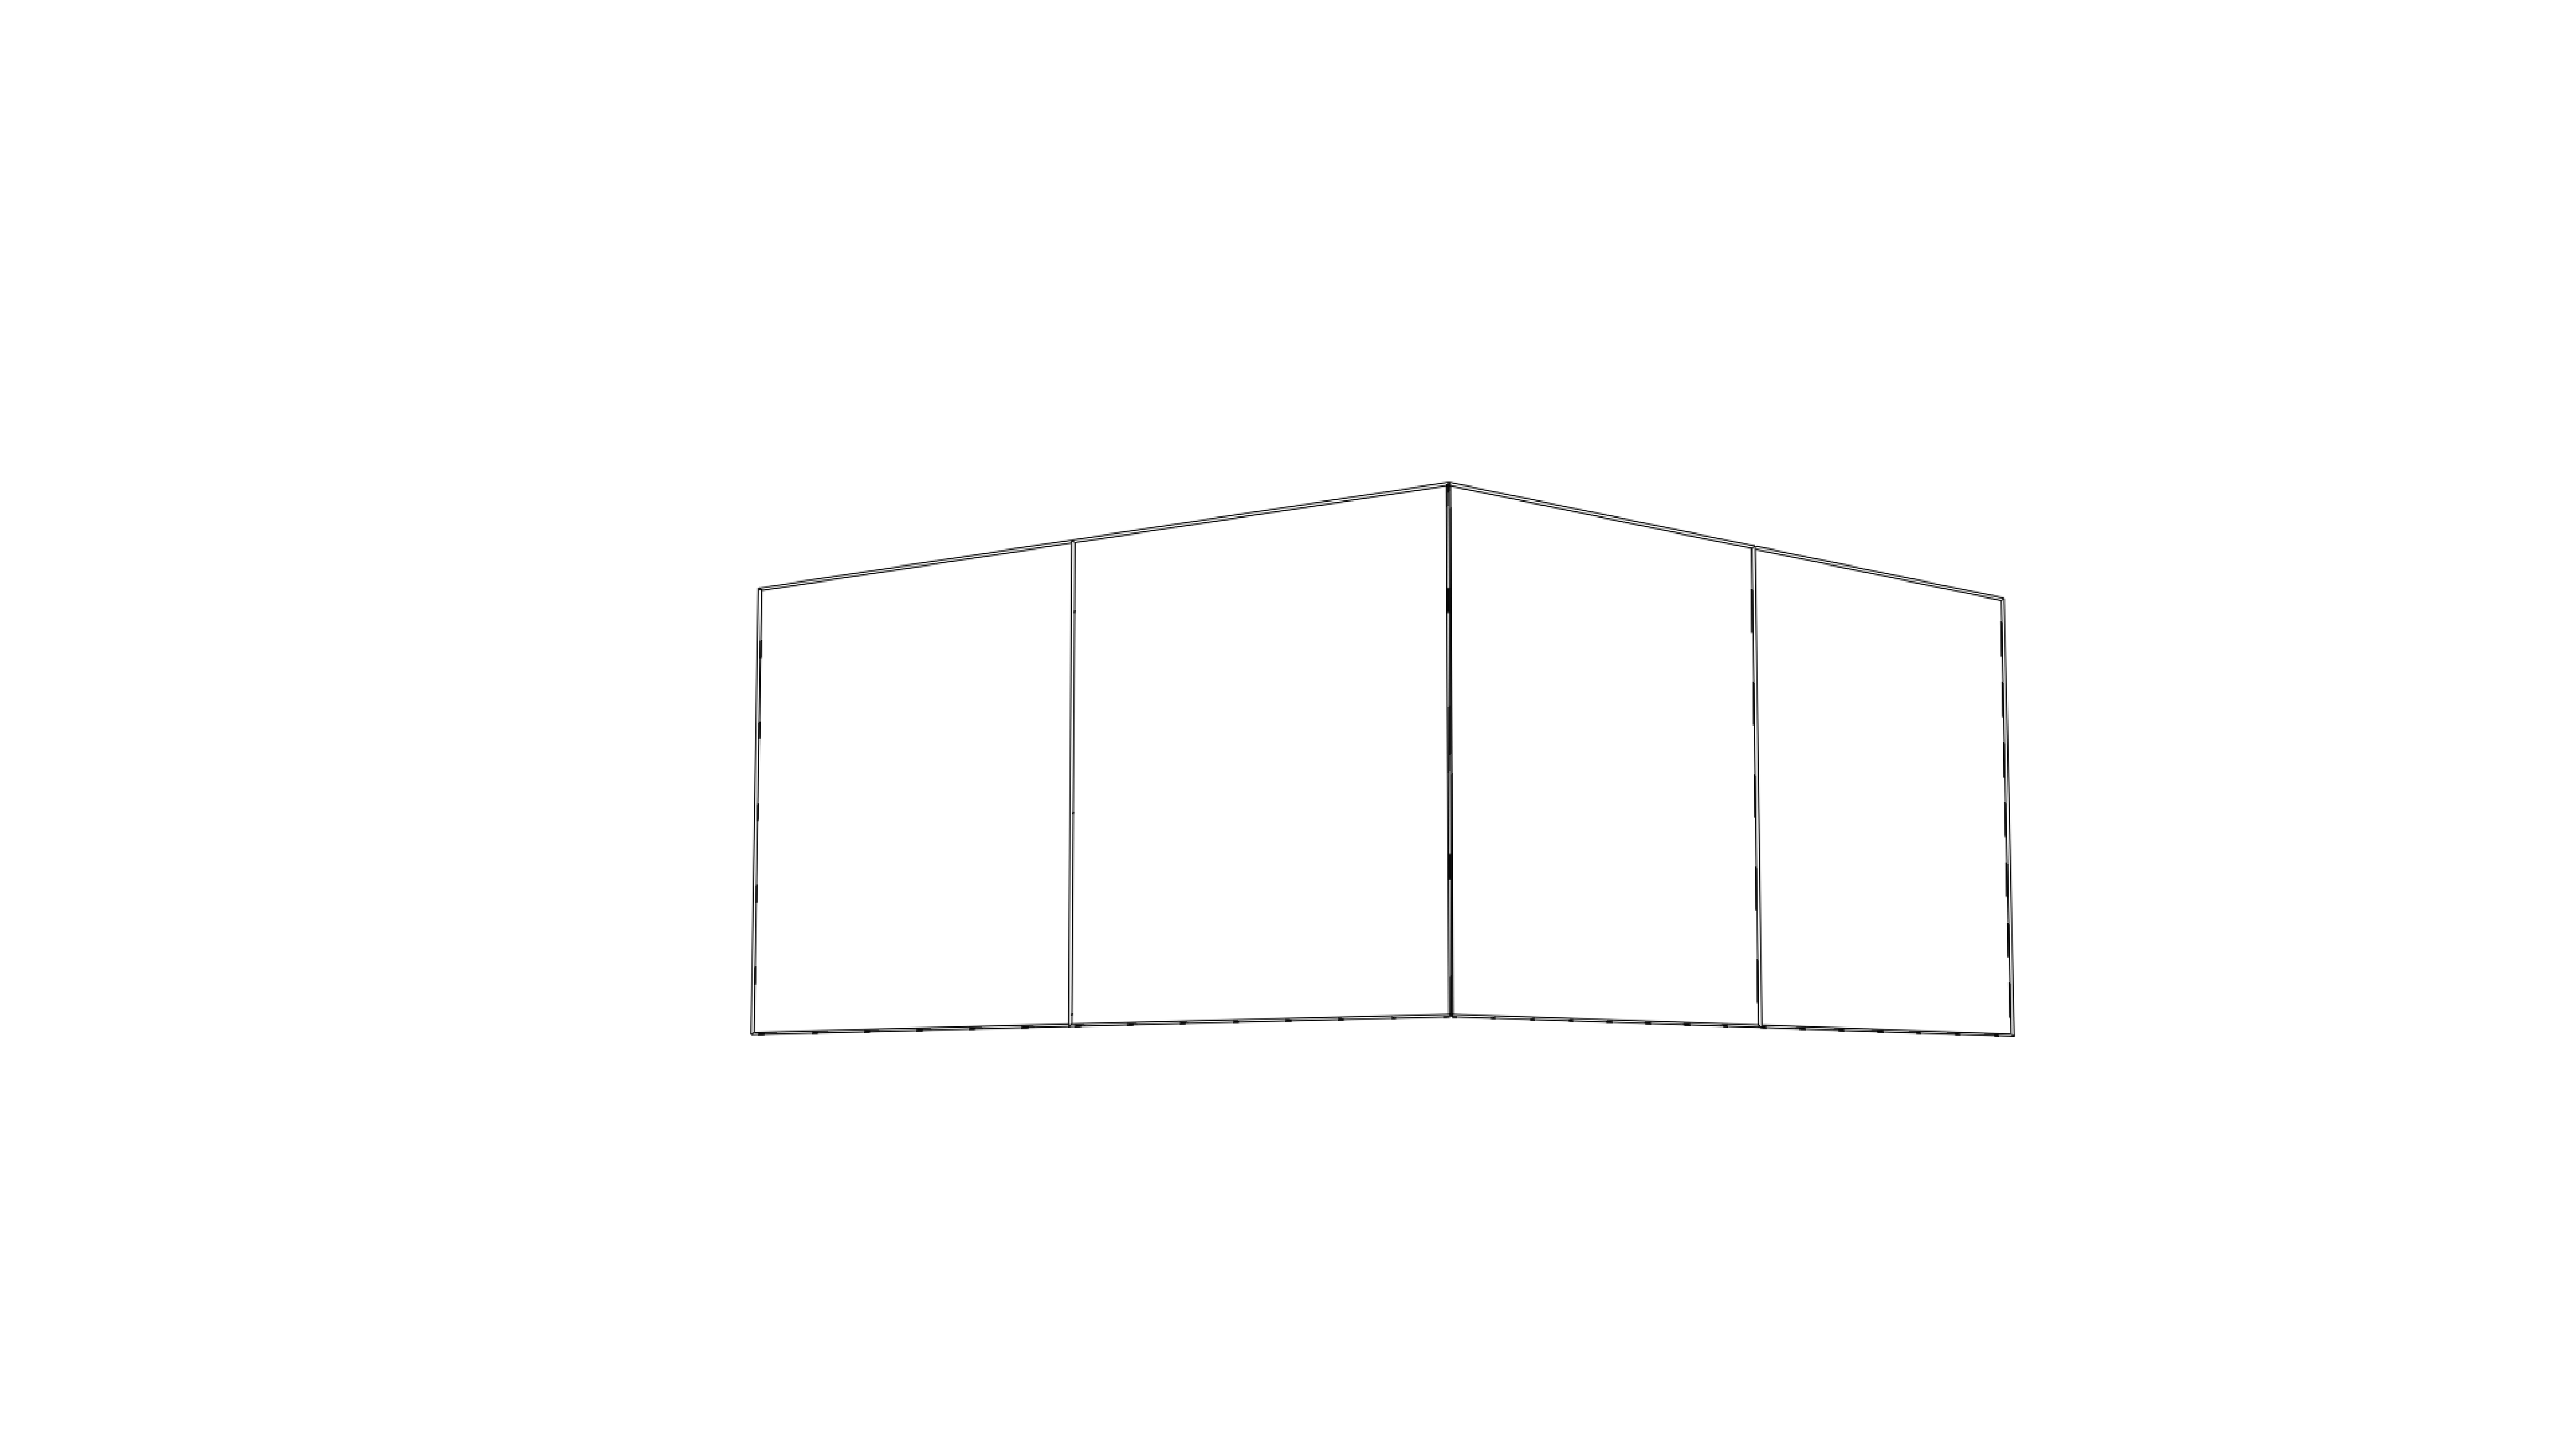
\includegraphics[width=1\linewidth]{Images/Wall 0/0001}} &
                {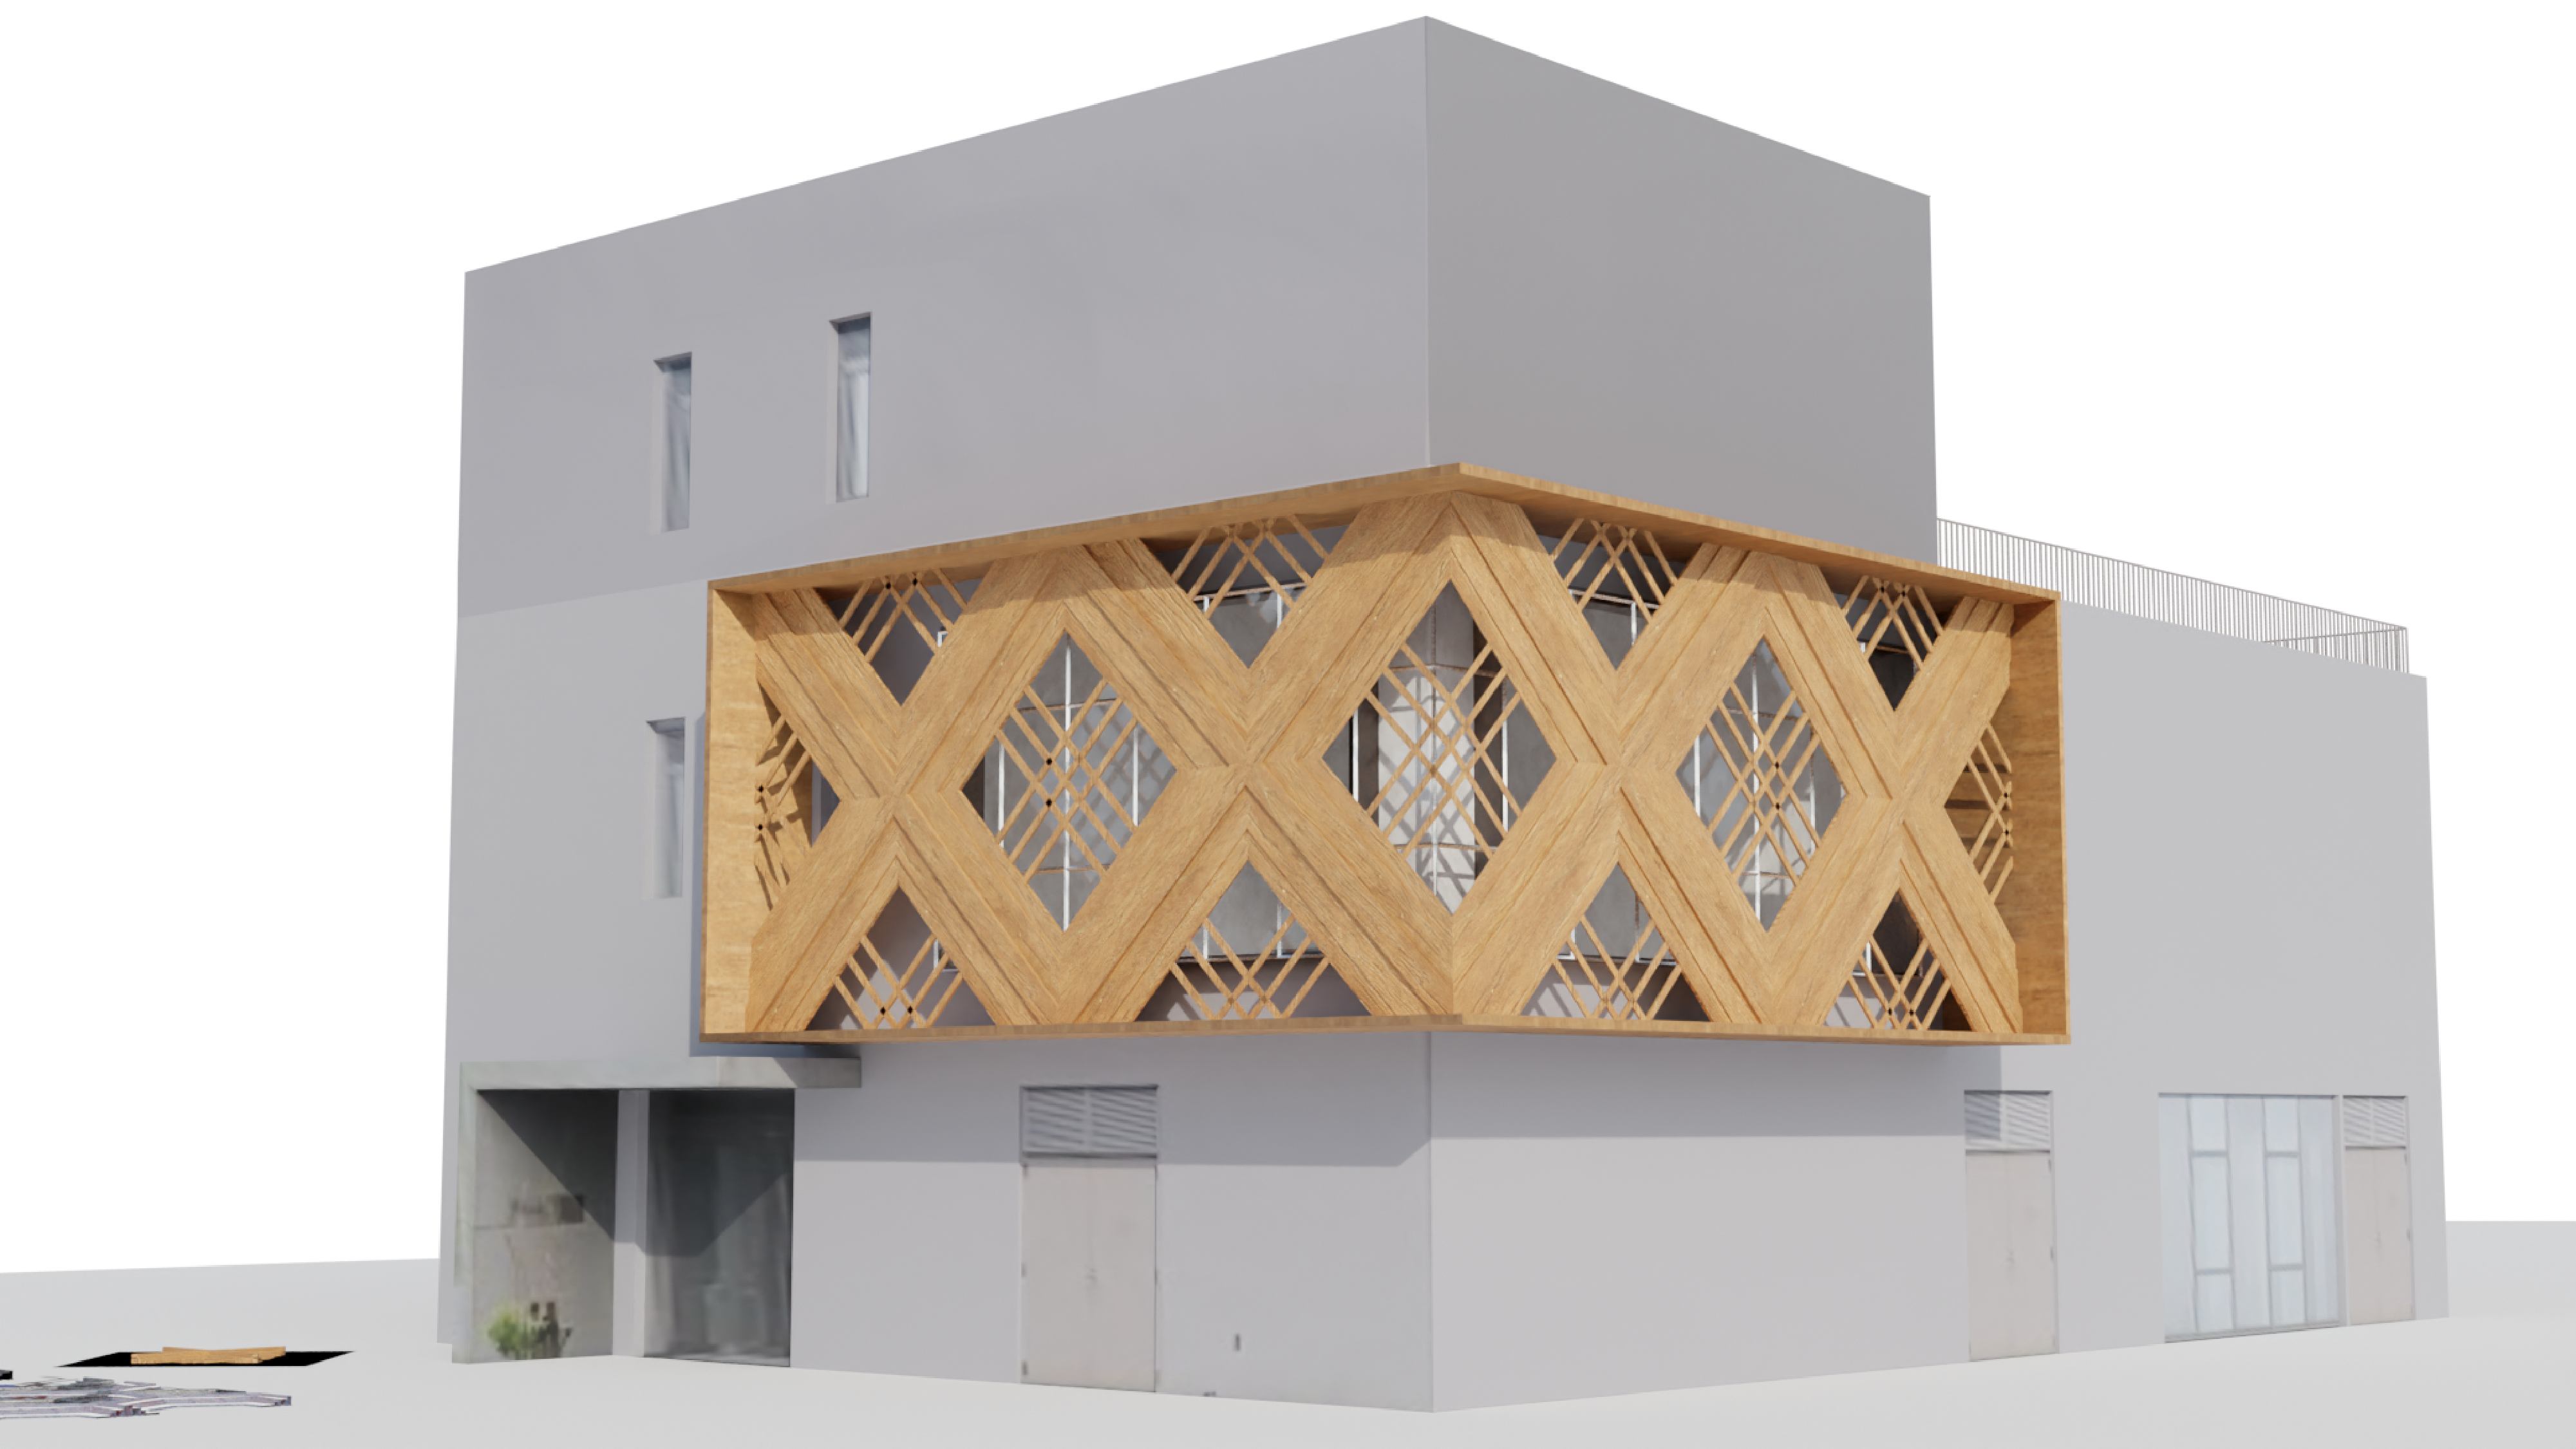
\includegraphics[width=1\linewidth]{Images/Pattern 1/0001}} &
              {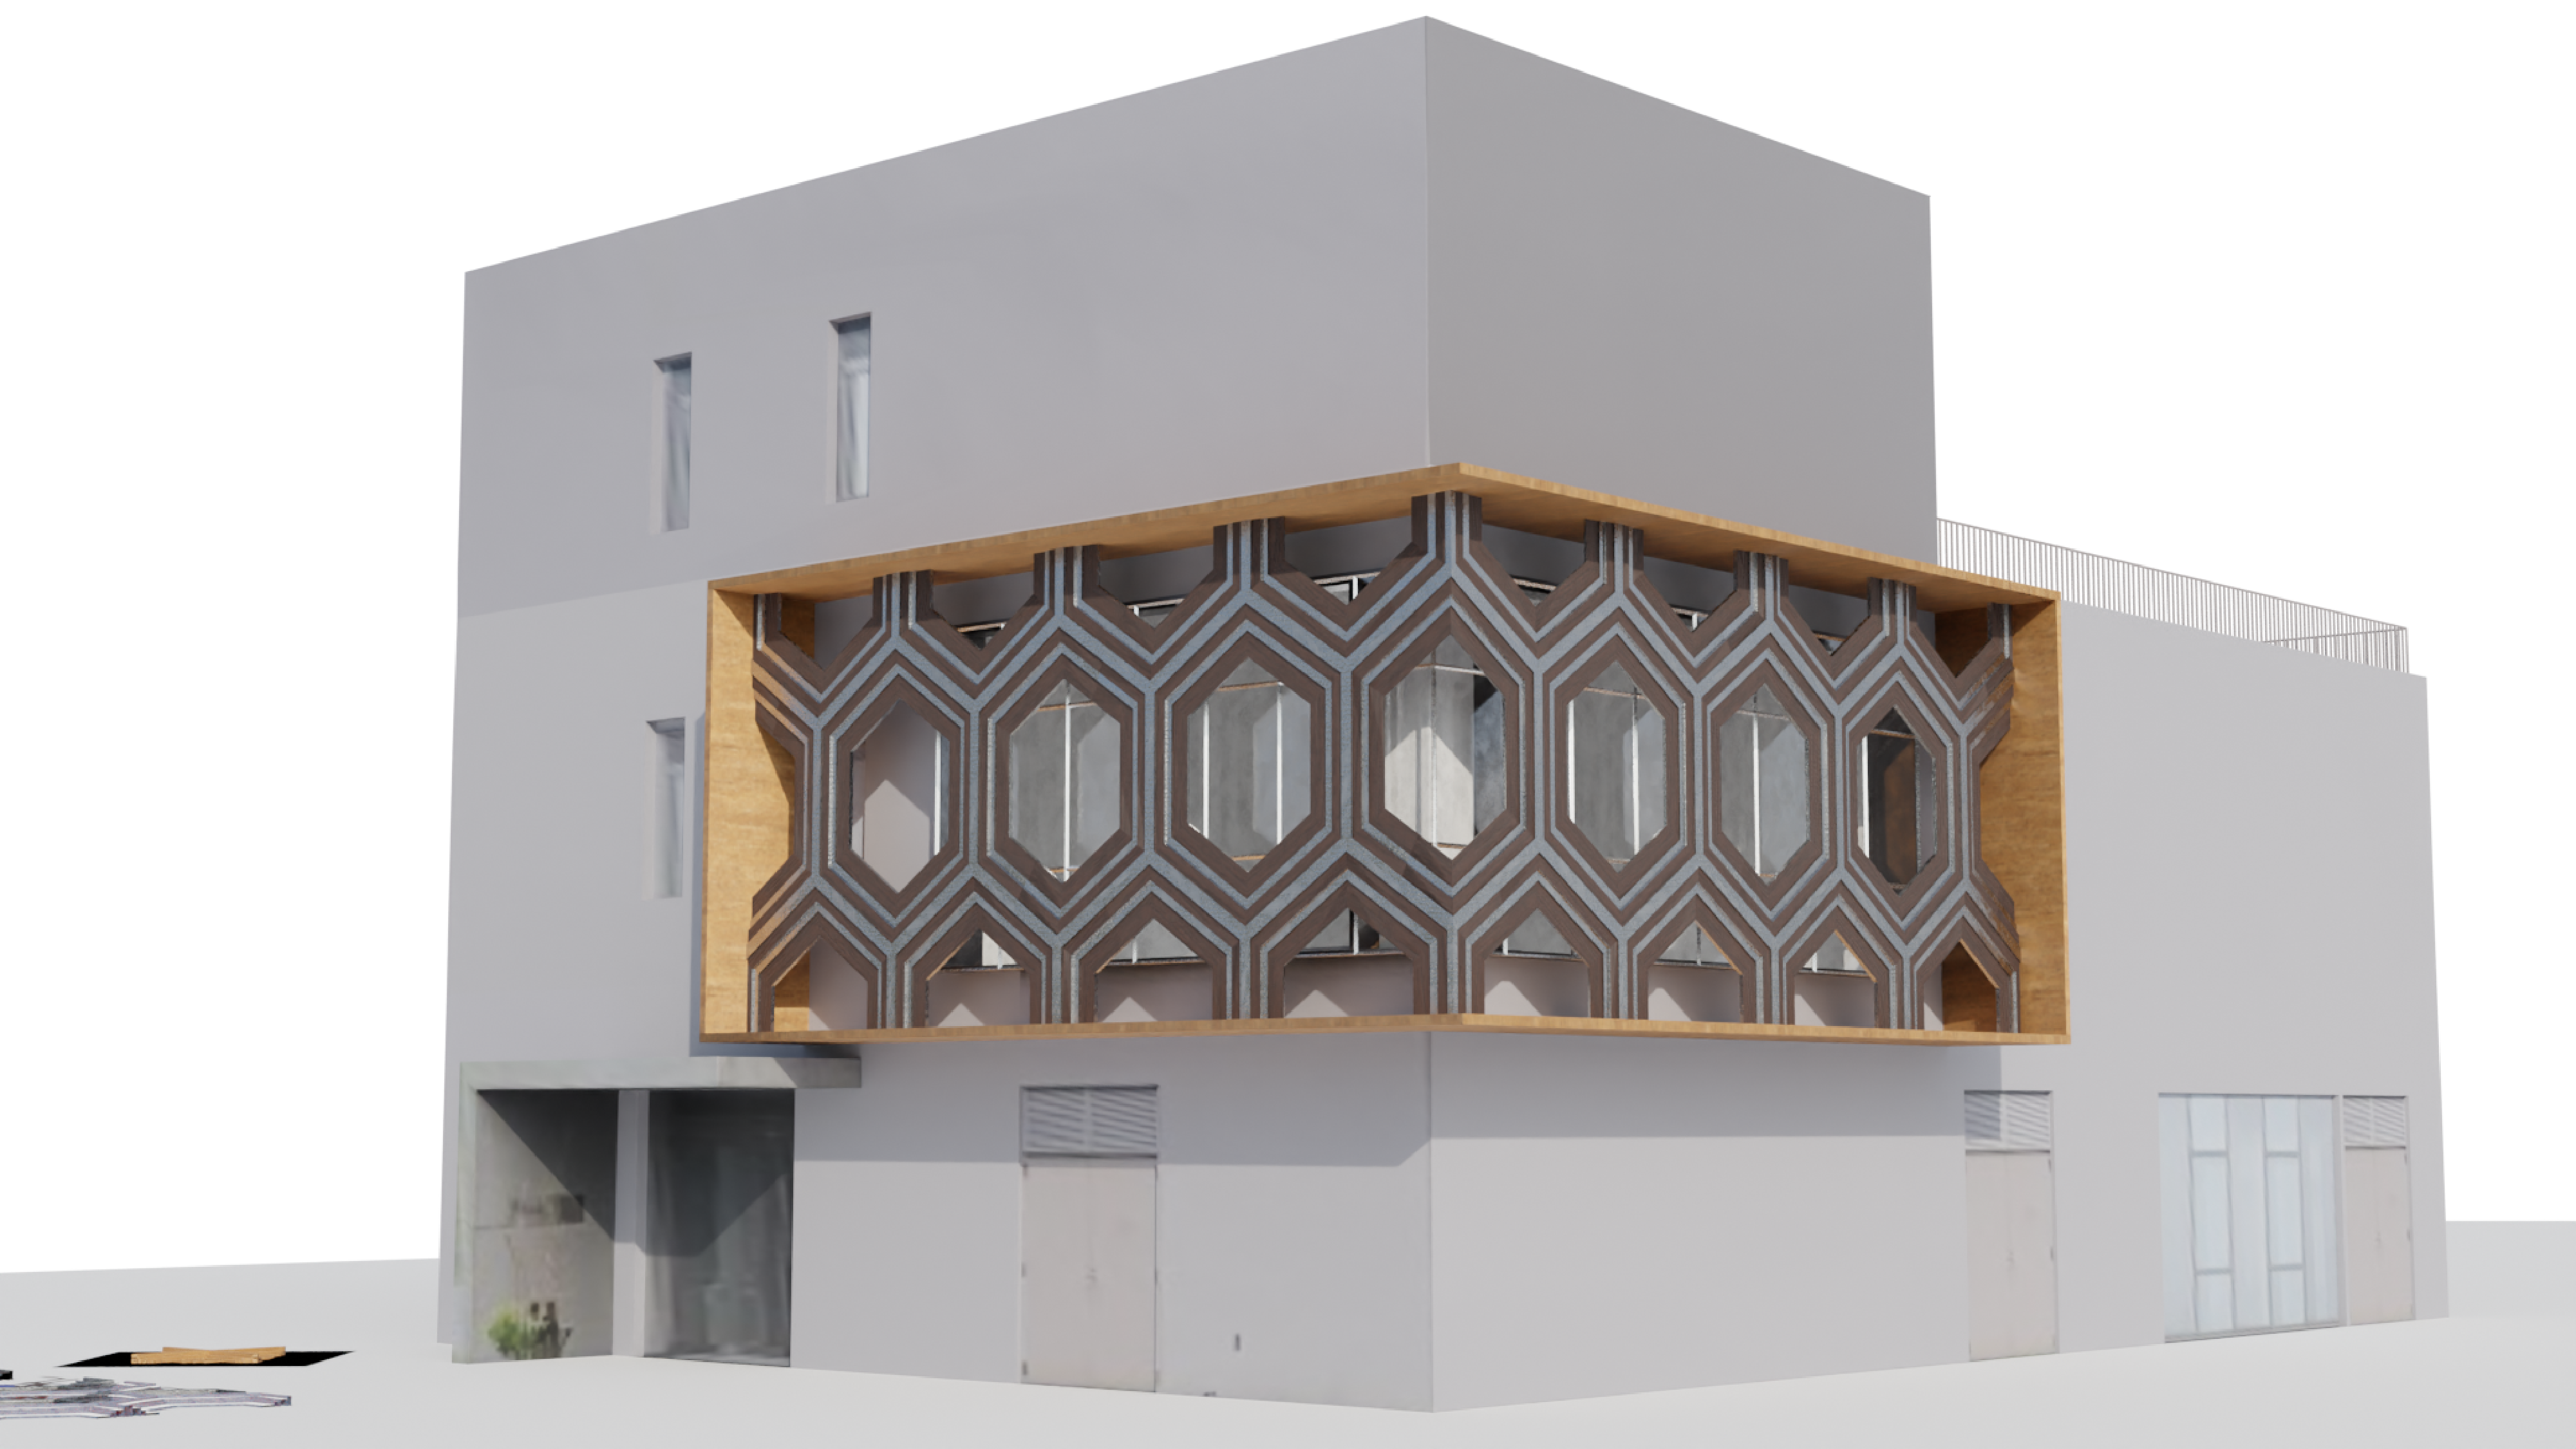
\includegraphics[width=1\linewidth]{Images/Pattern 2/0001}} &
              {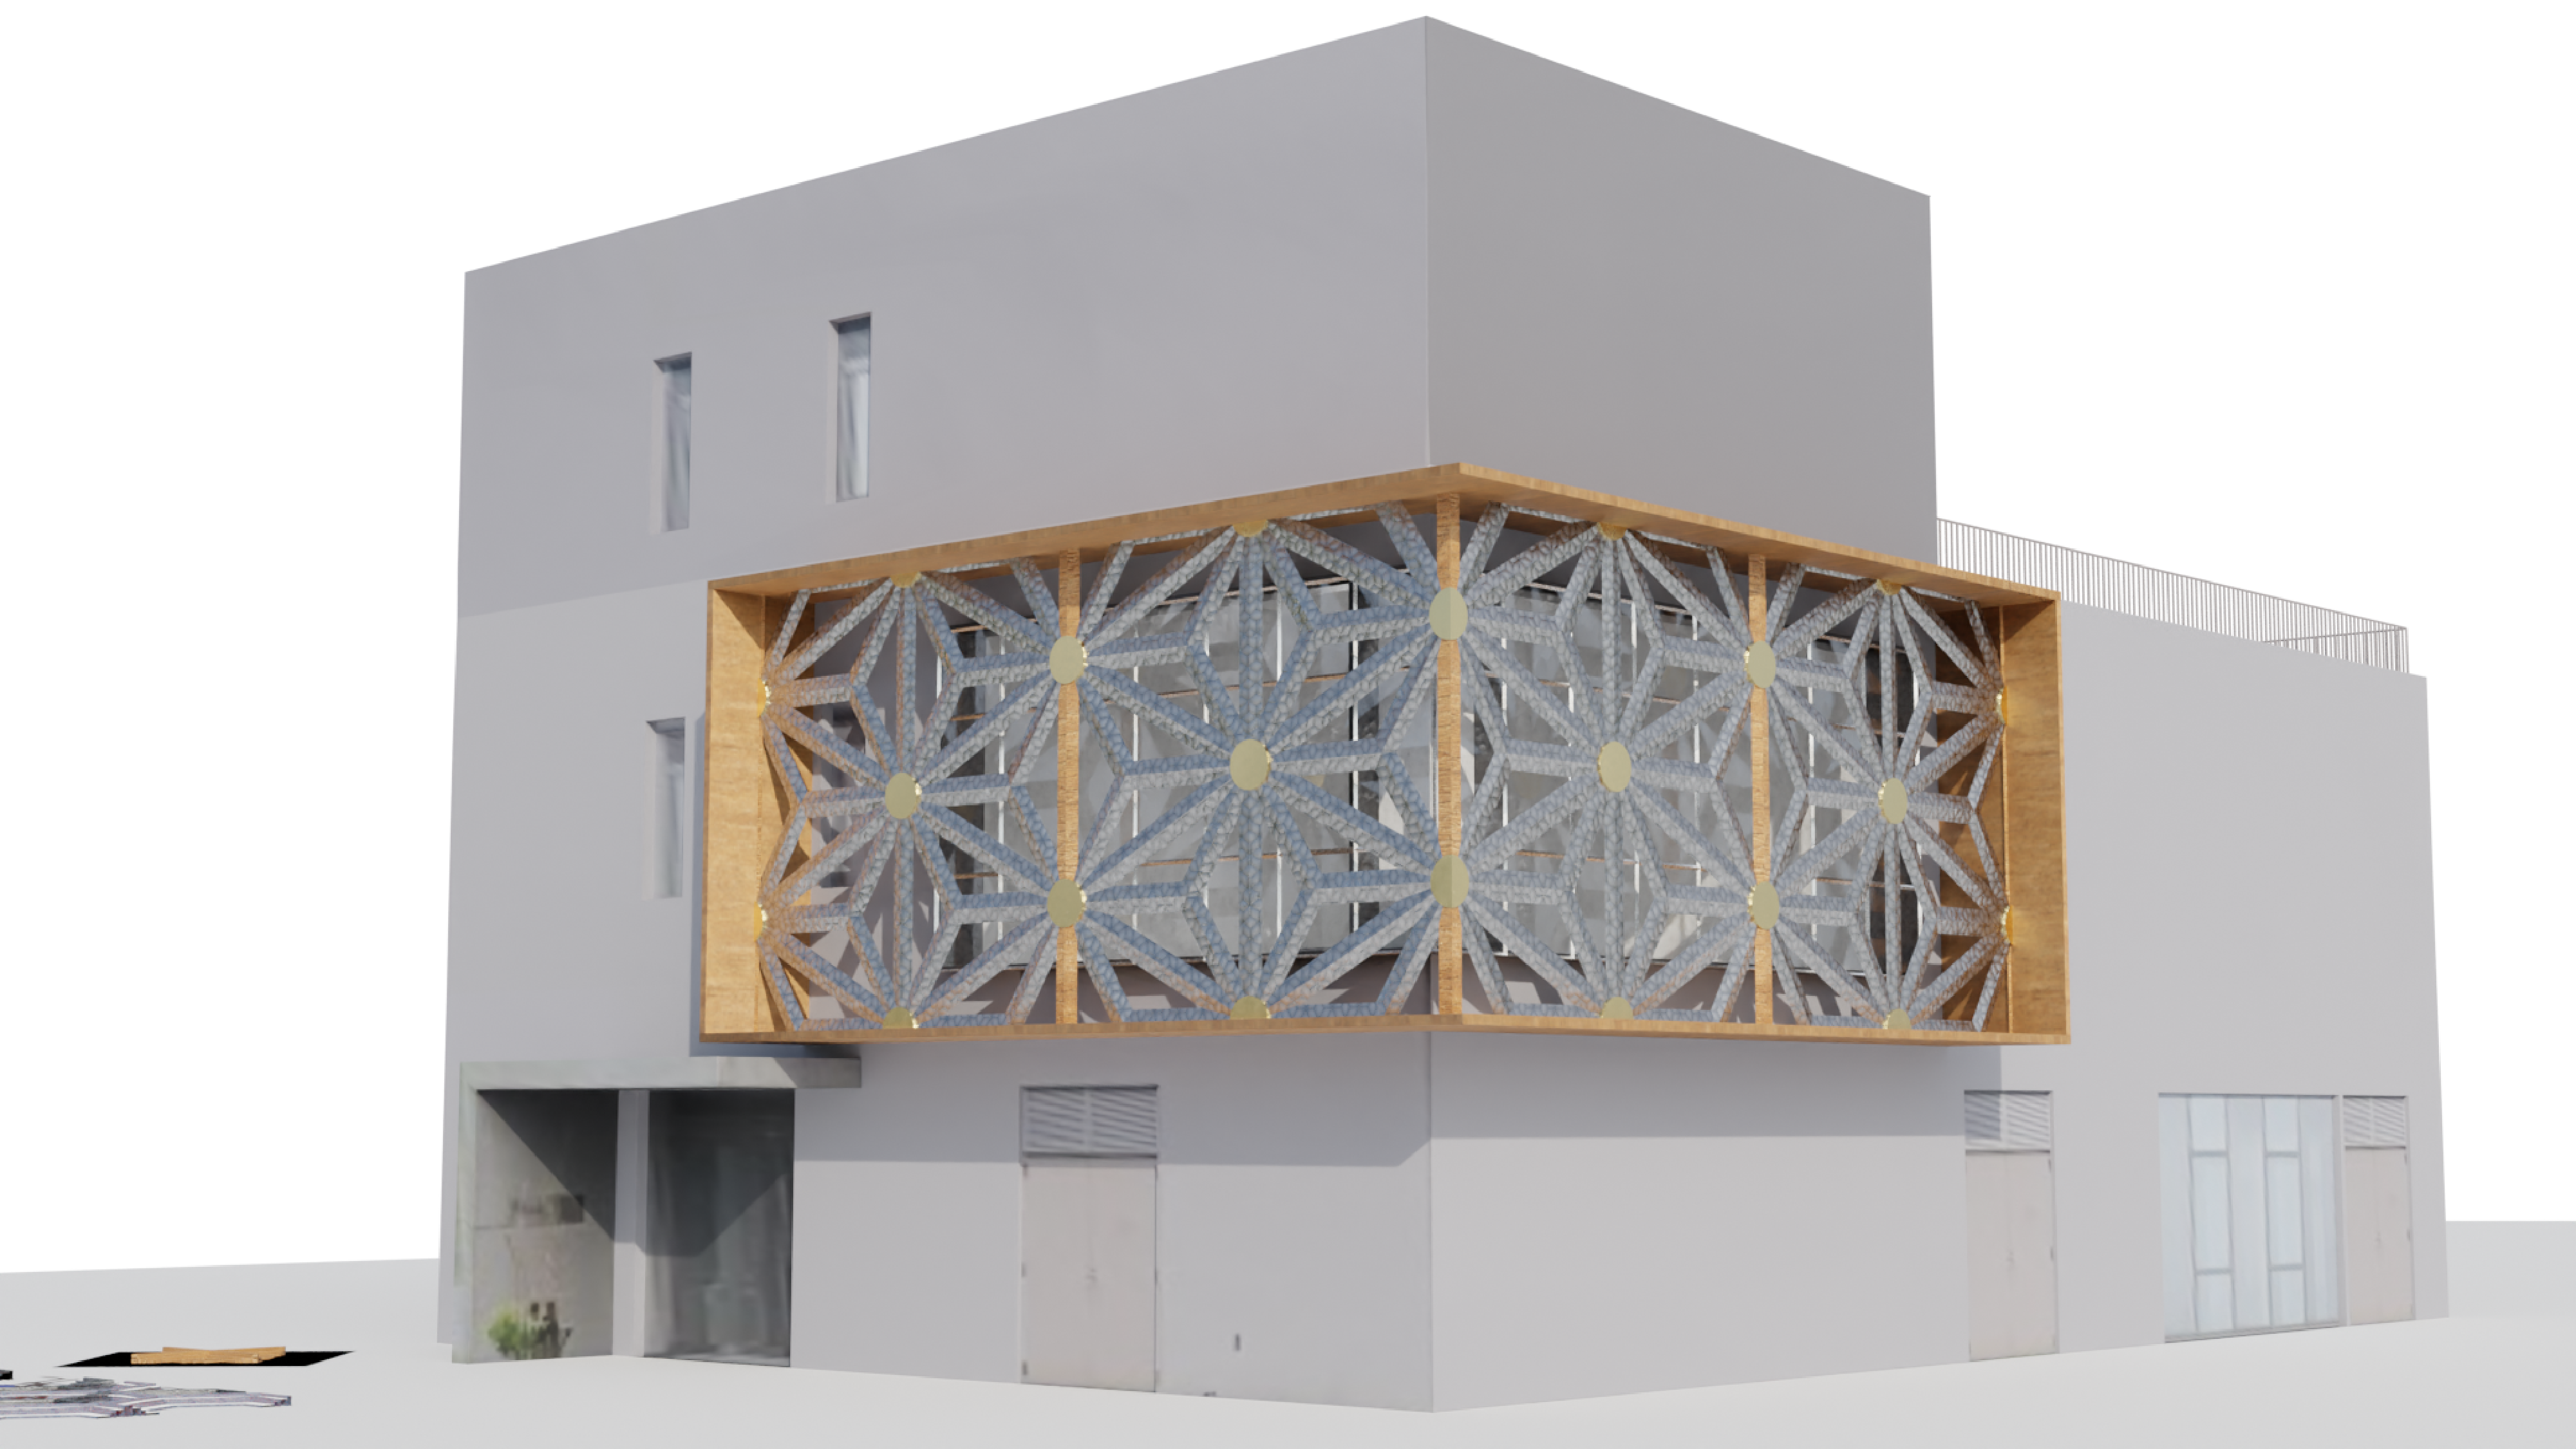
\includegraphics[width=1\linewidth]{Images/Pattern 3/0001}} \\
            \midrule
            \textit{Level 2} &  &  &
            \\
            {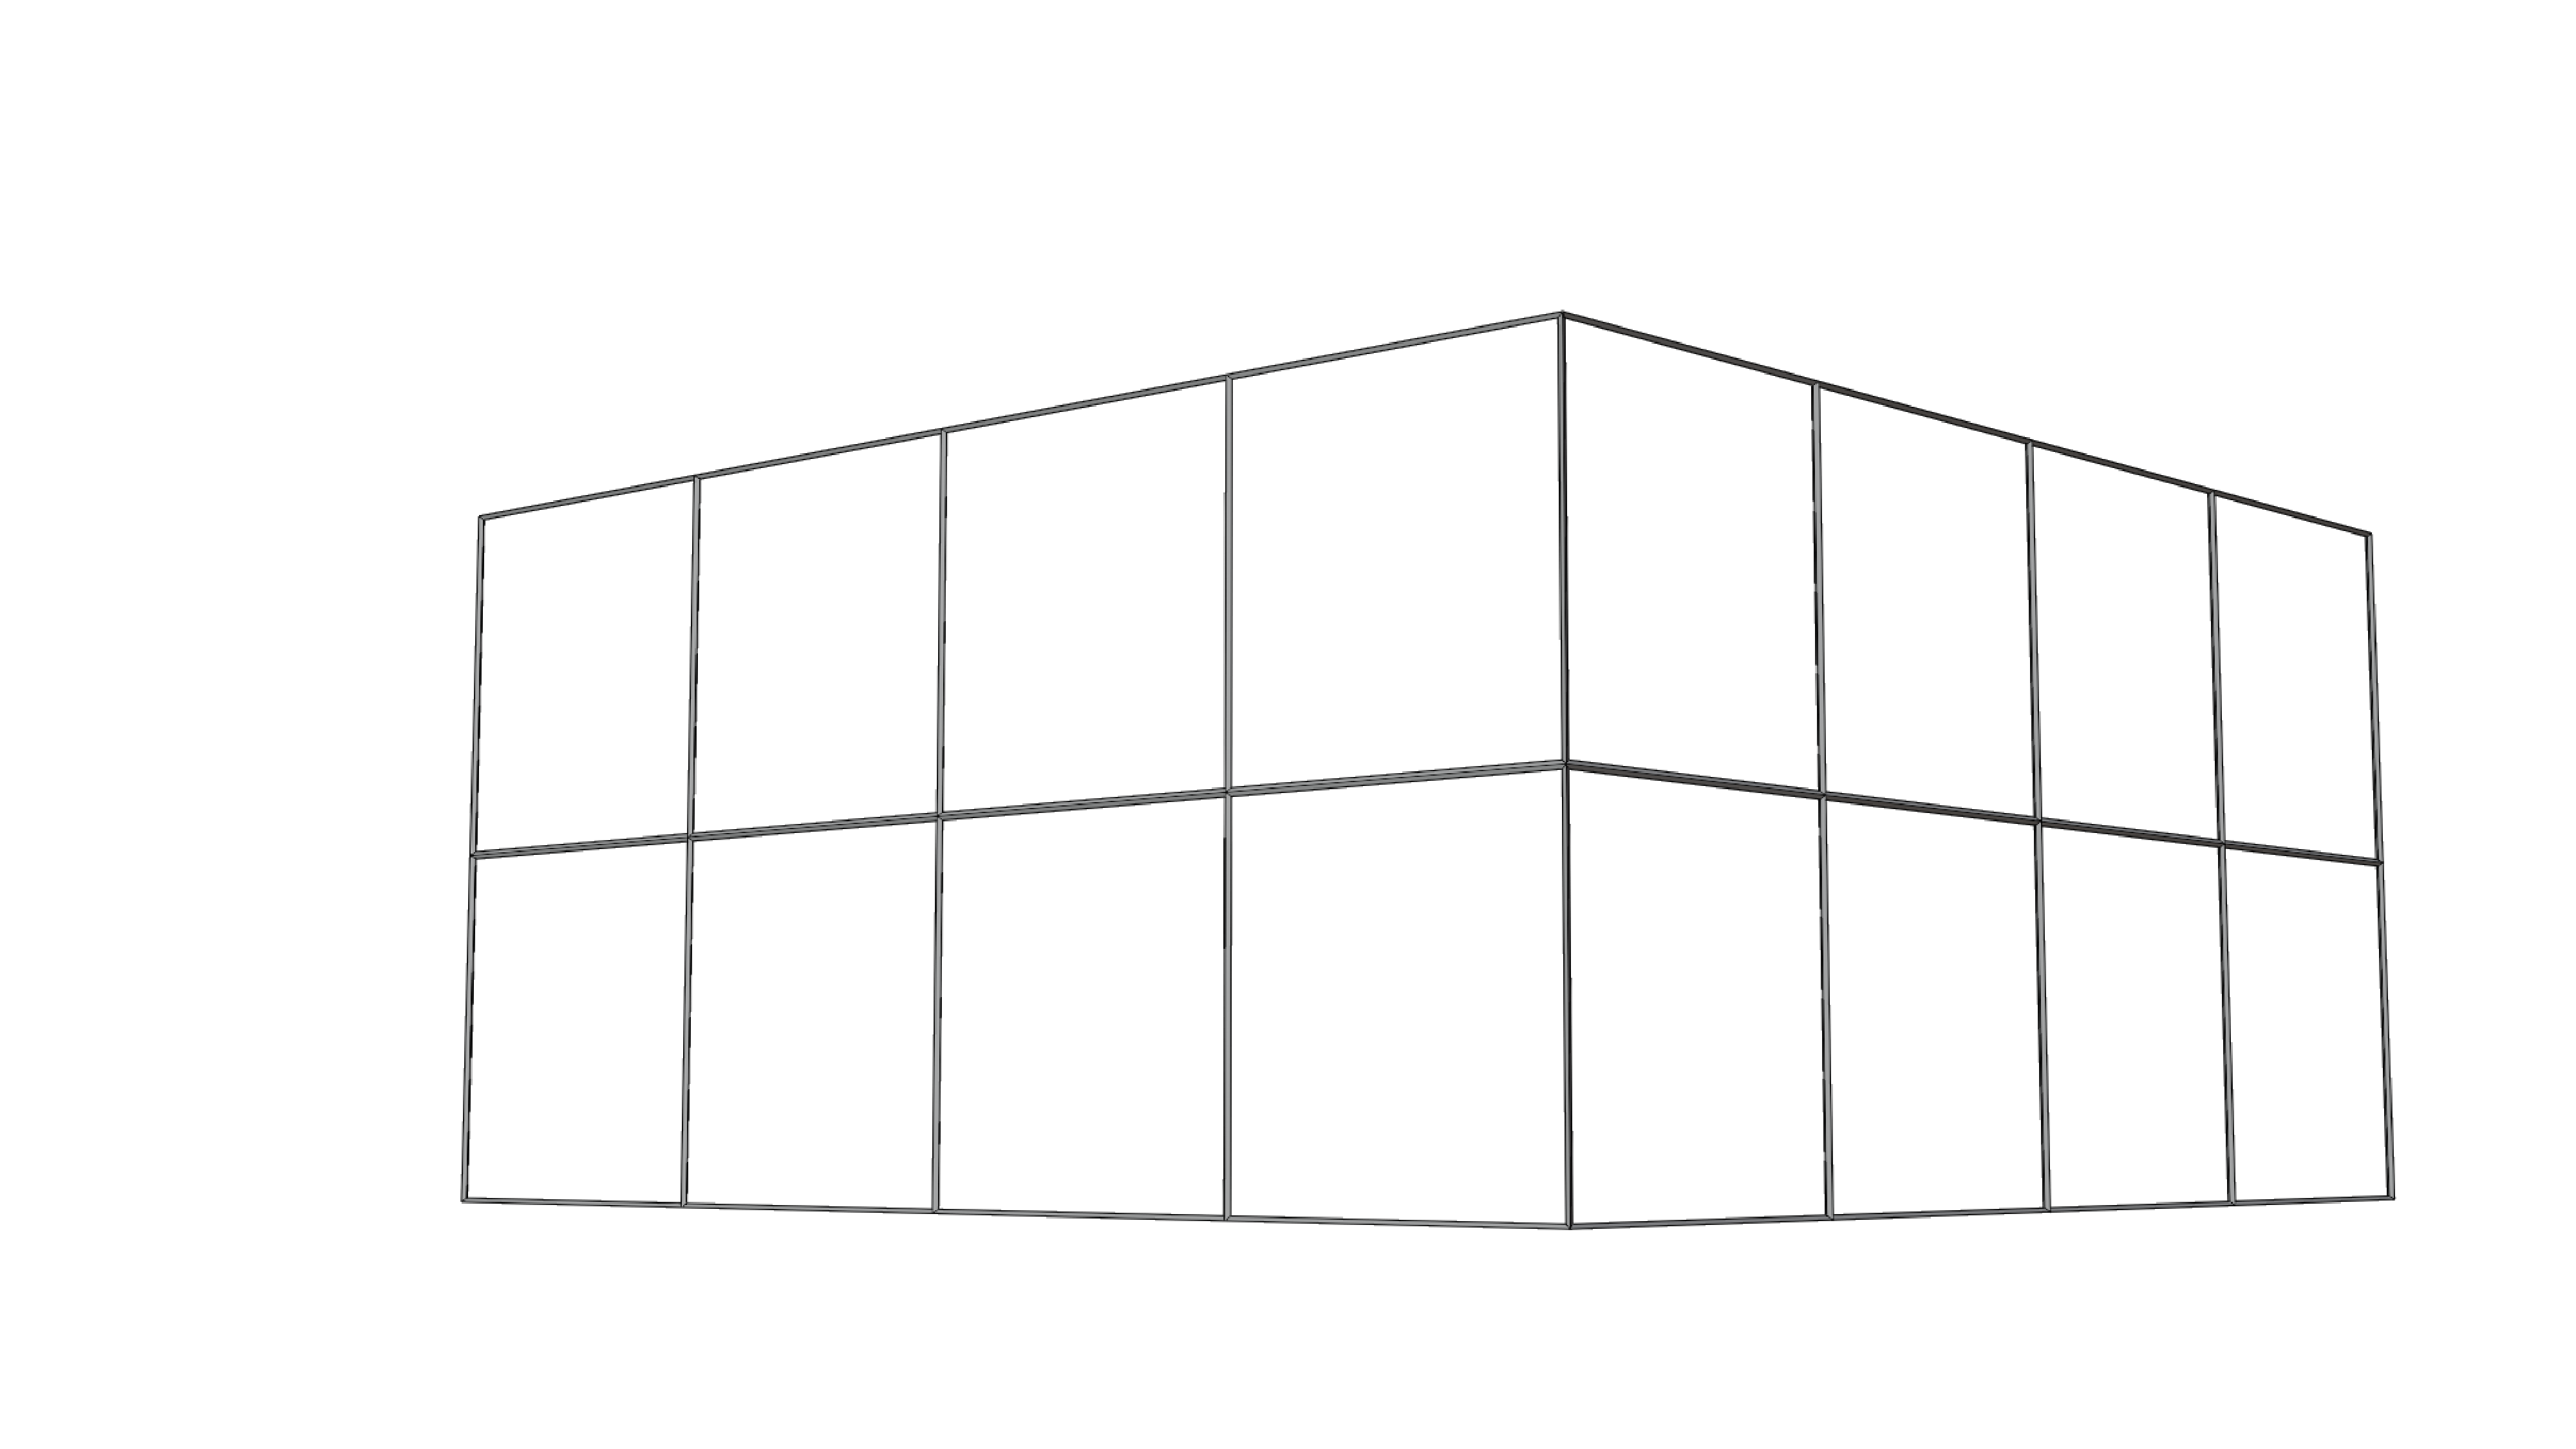
\includegraphics[width=1\linewidth]{Images/Wall 0/0002}} &
              {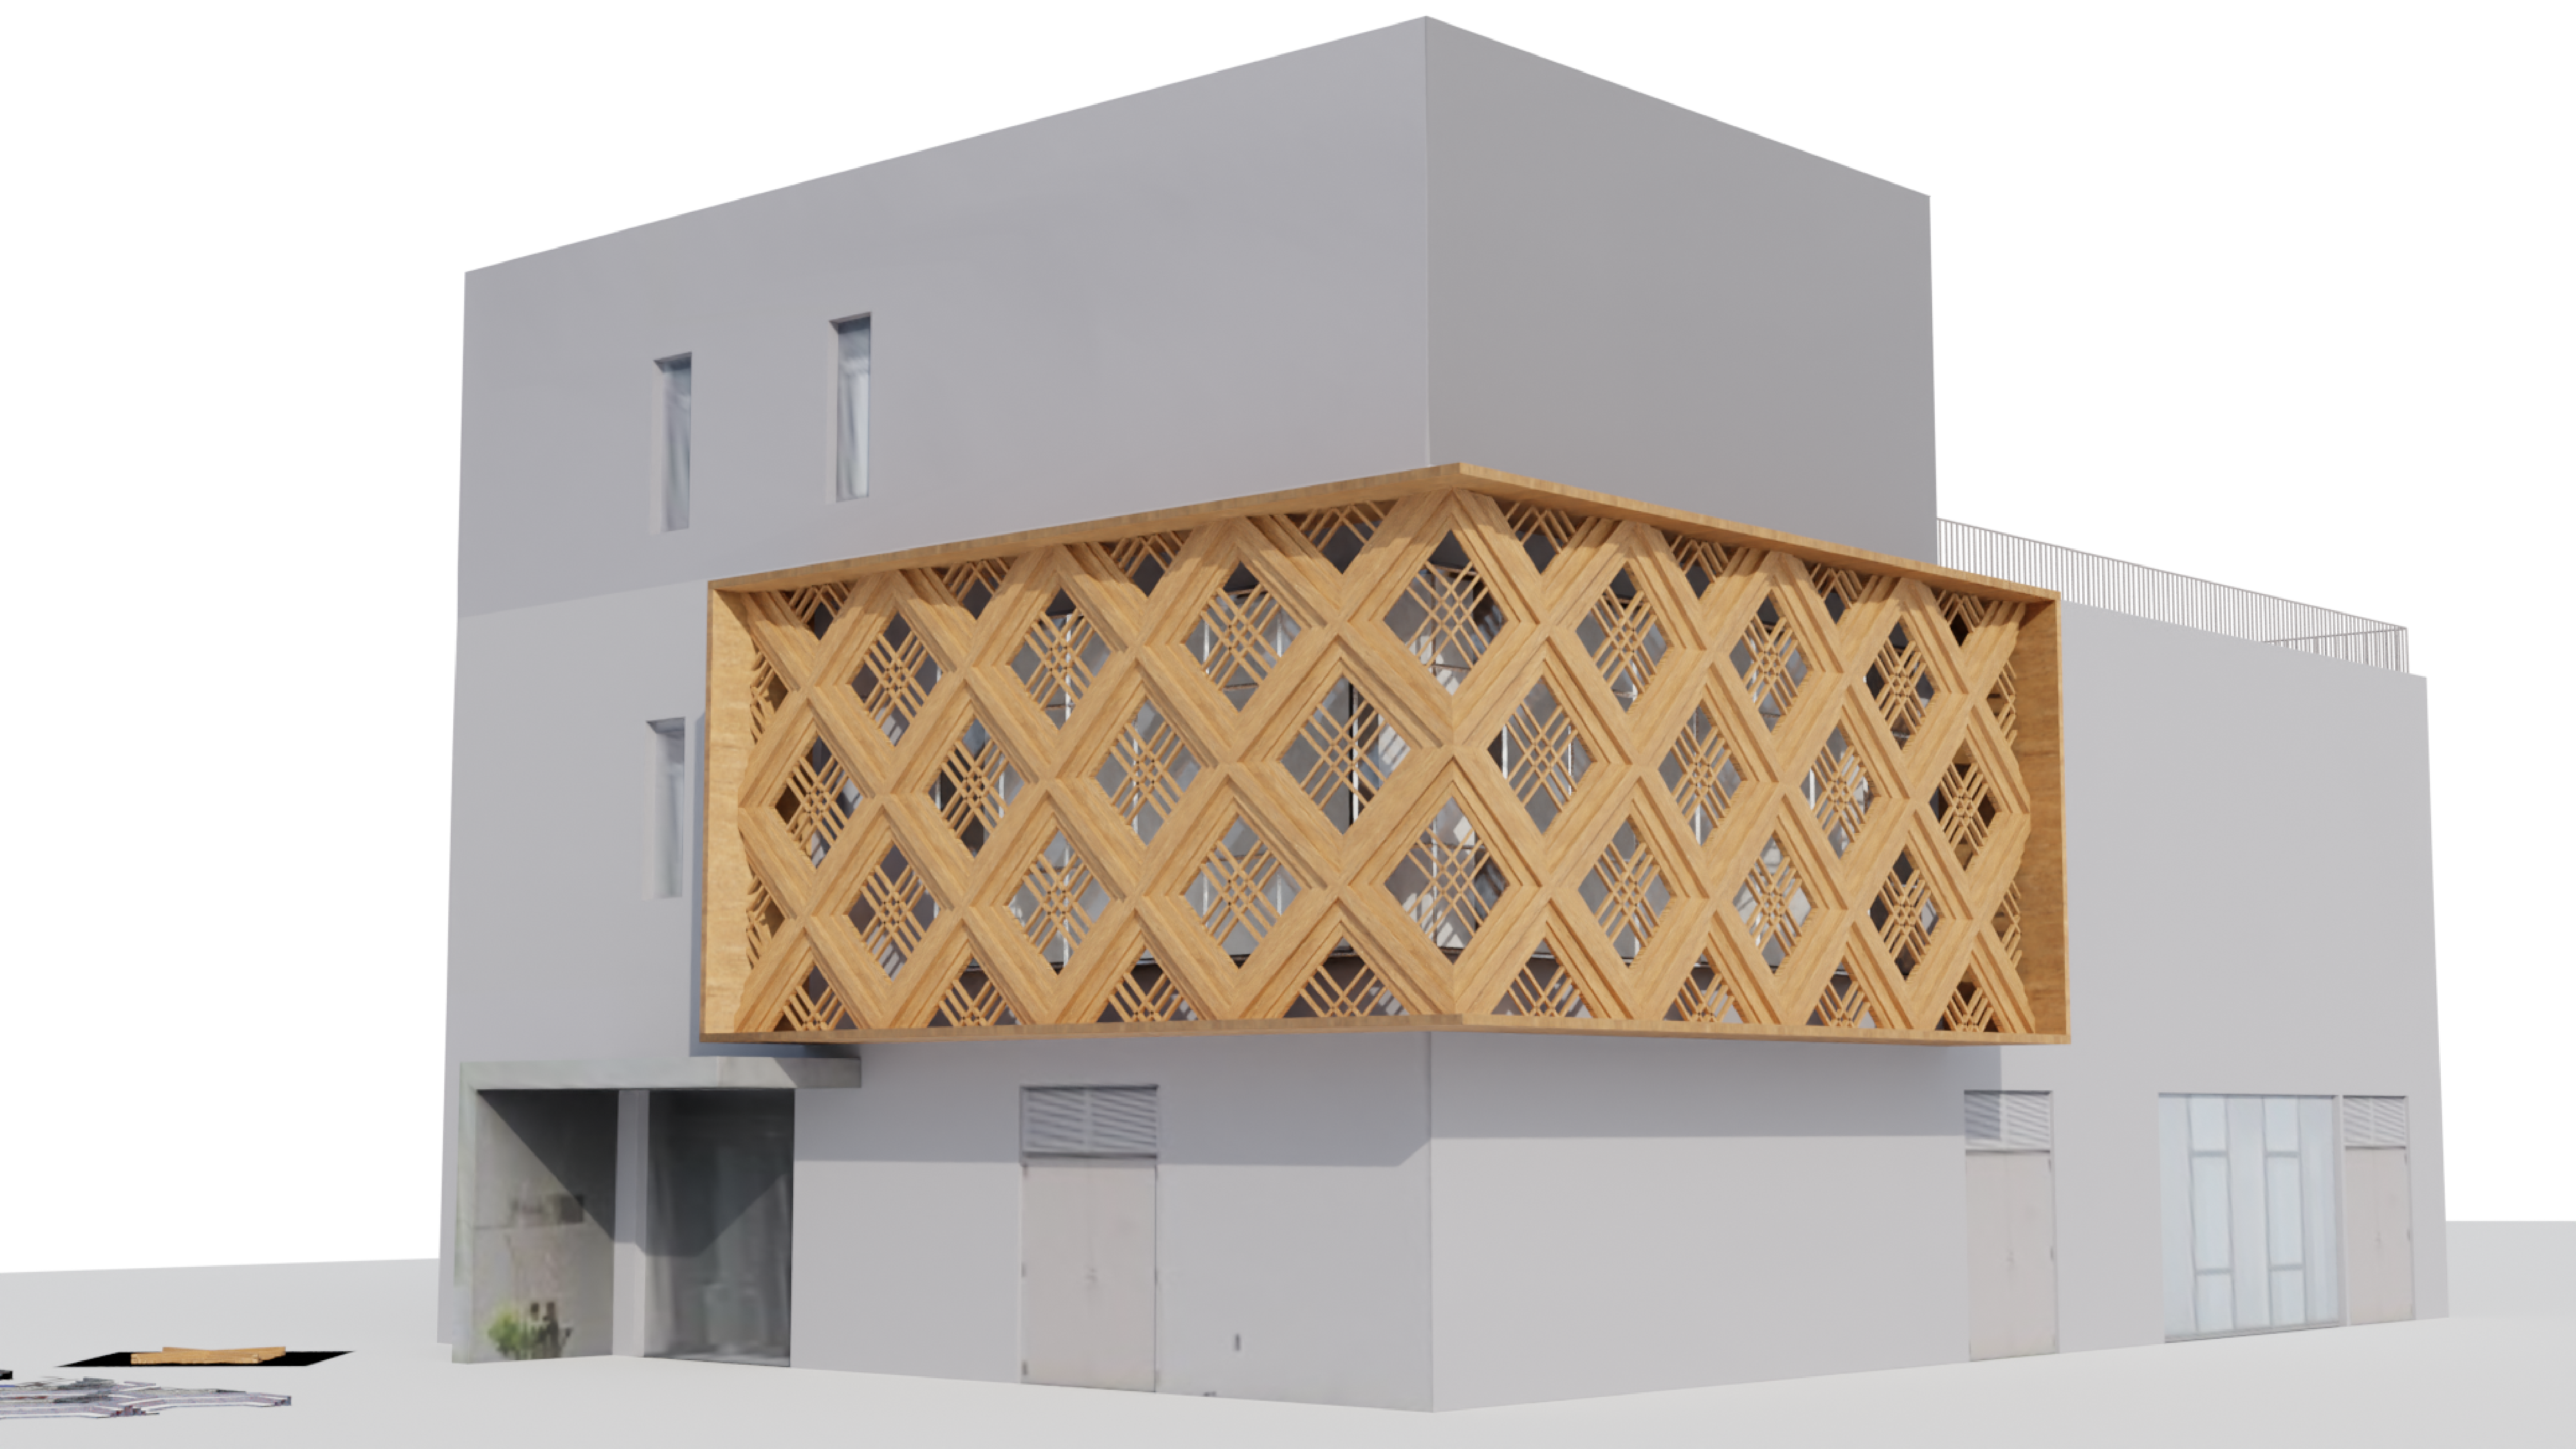
\includegraphics[width=1\linewidth]{Images/Pattern 1/0002}} &
              {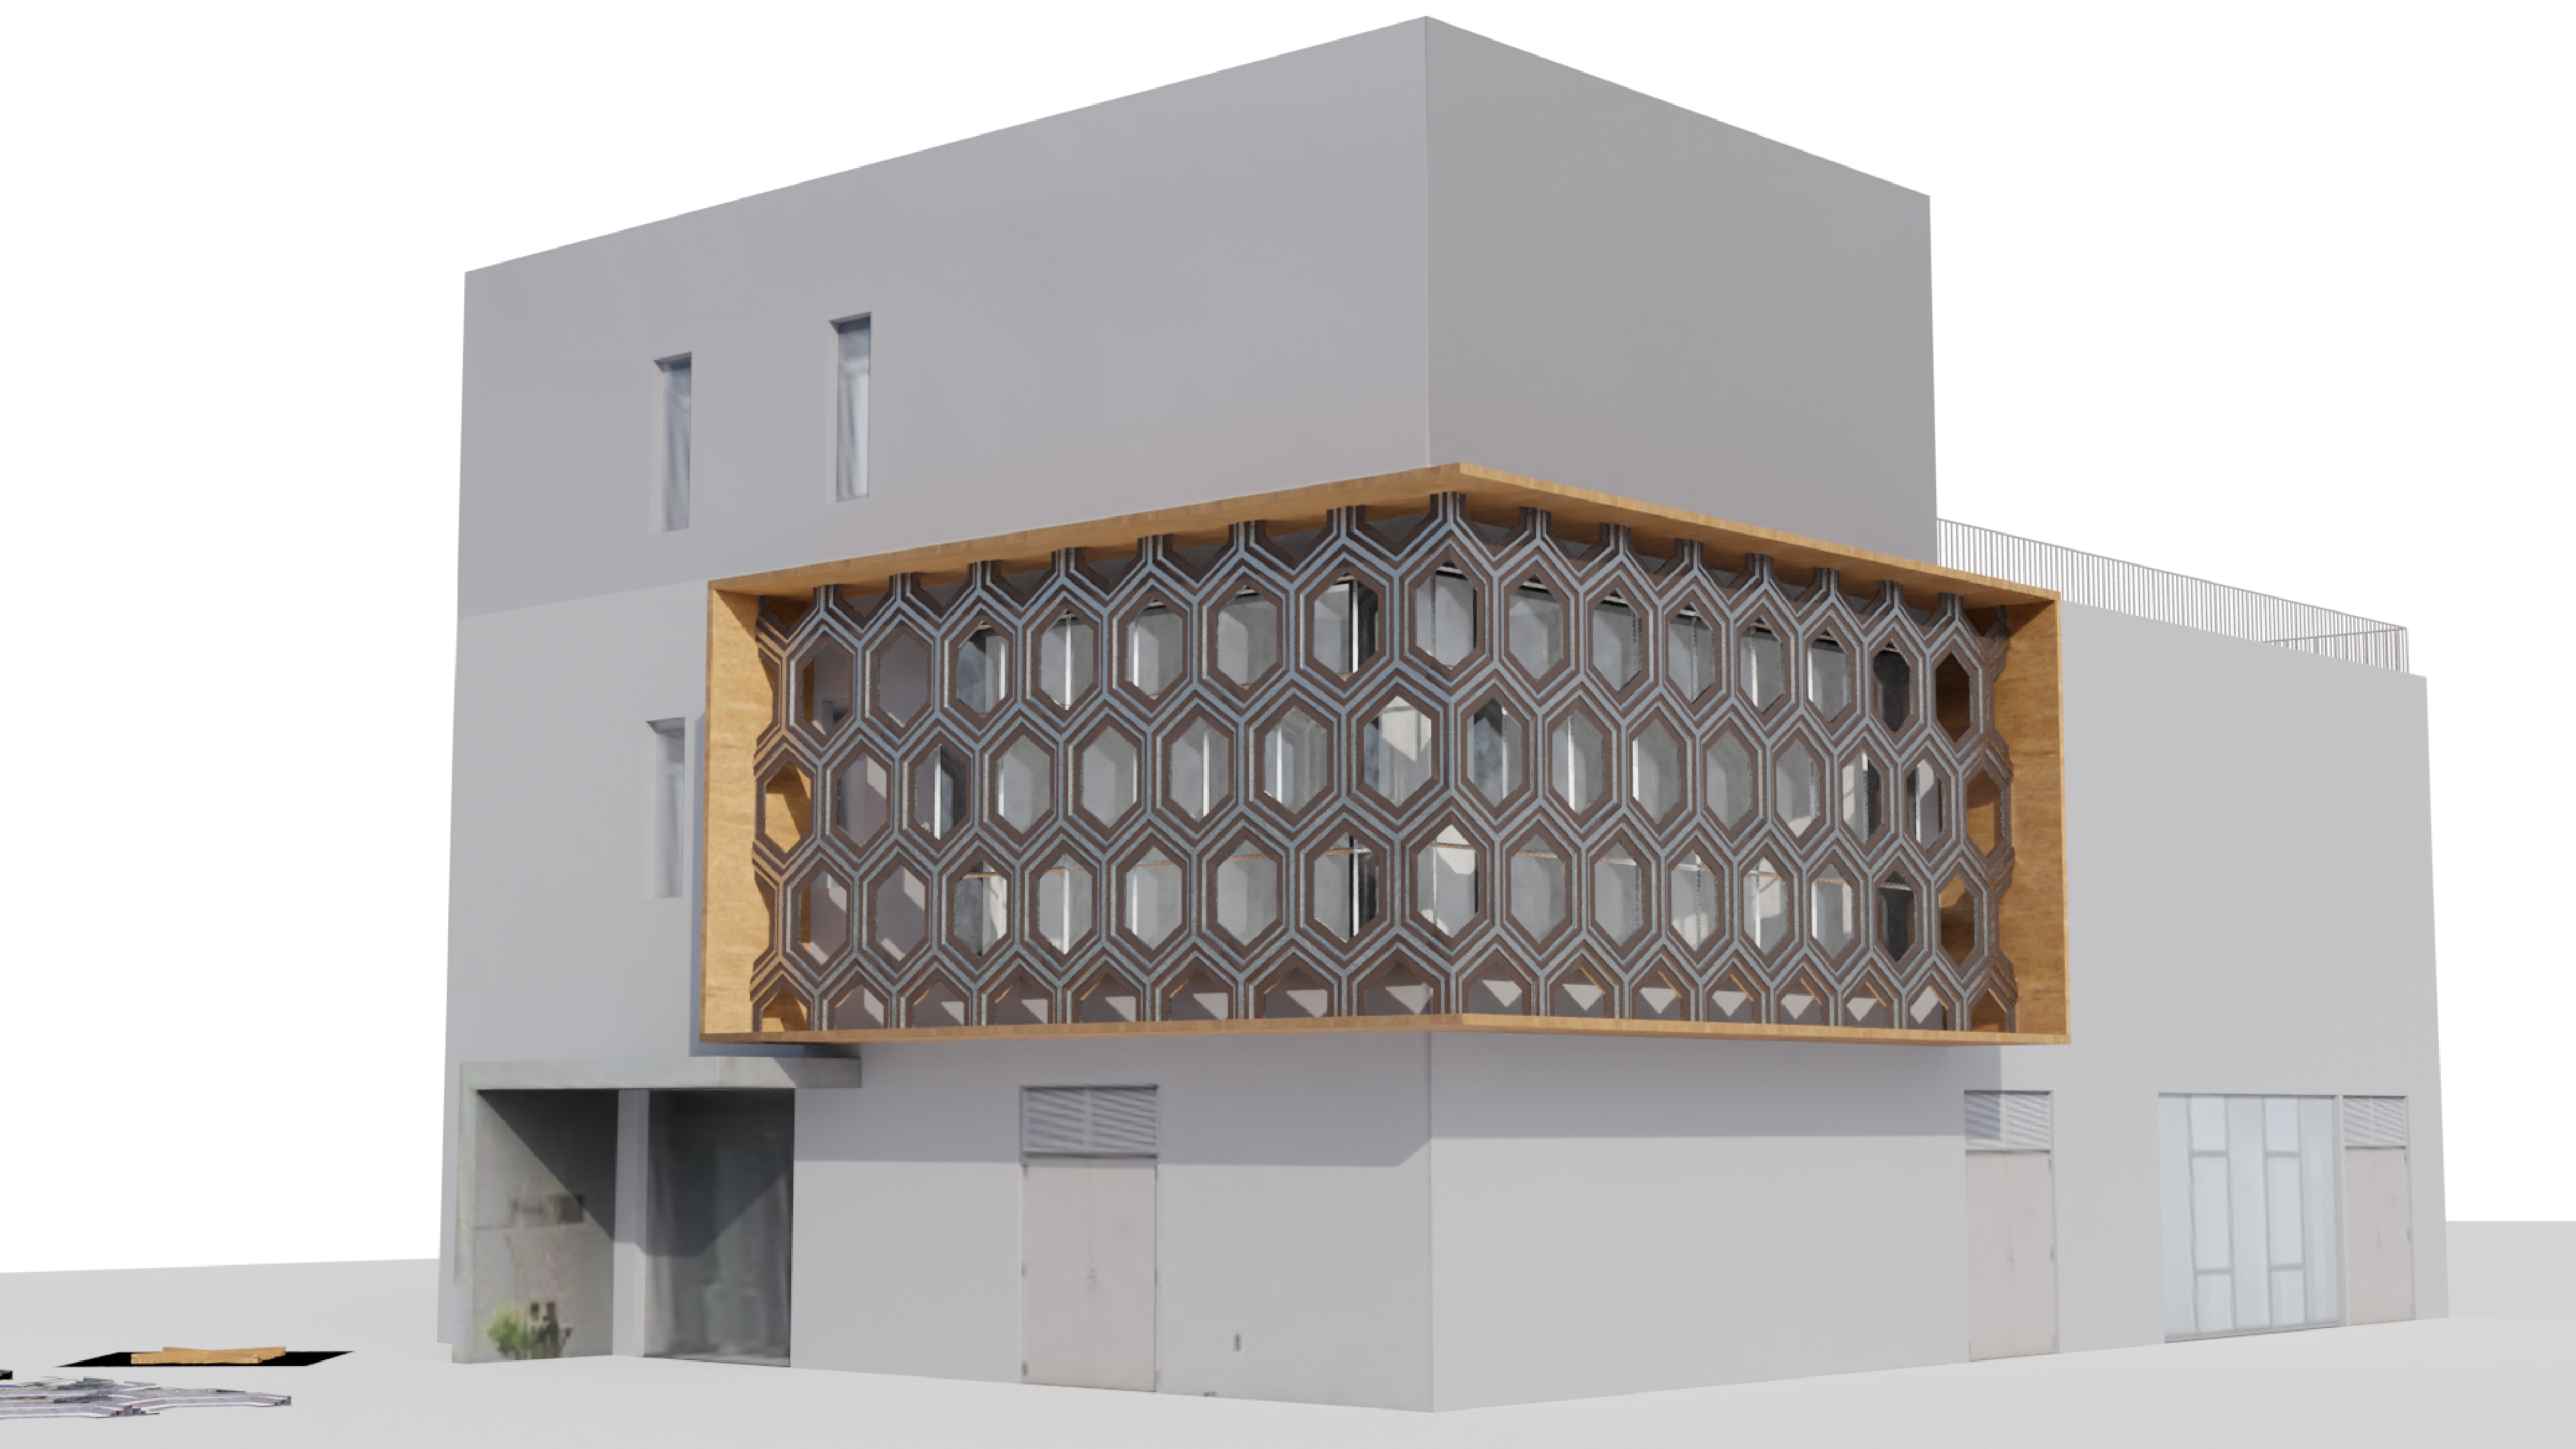
\includegraphics[width=1\linewidth]{Images/Pattern 2/0002}} &
              {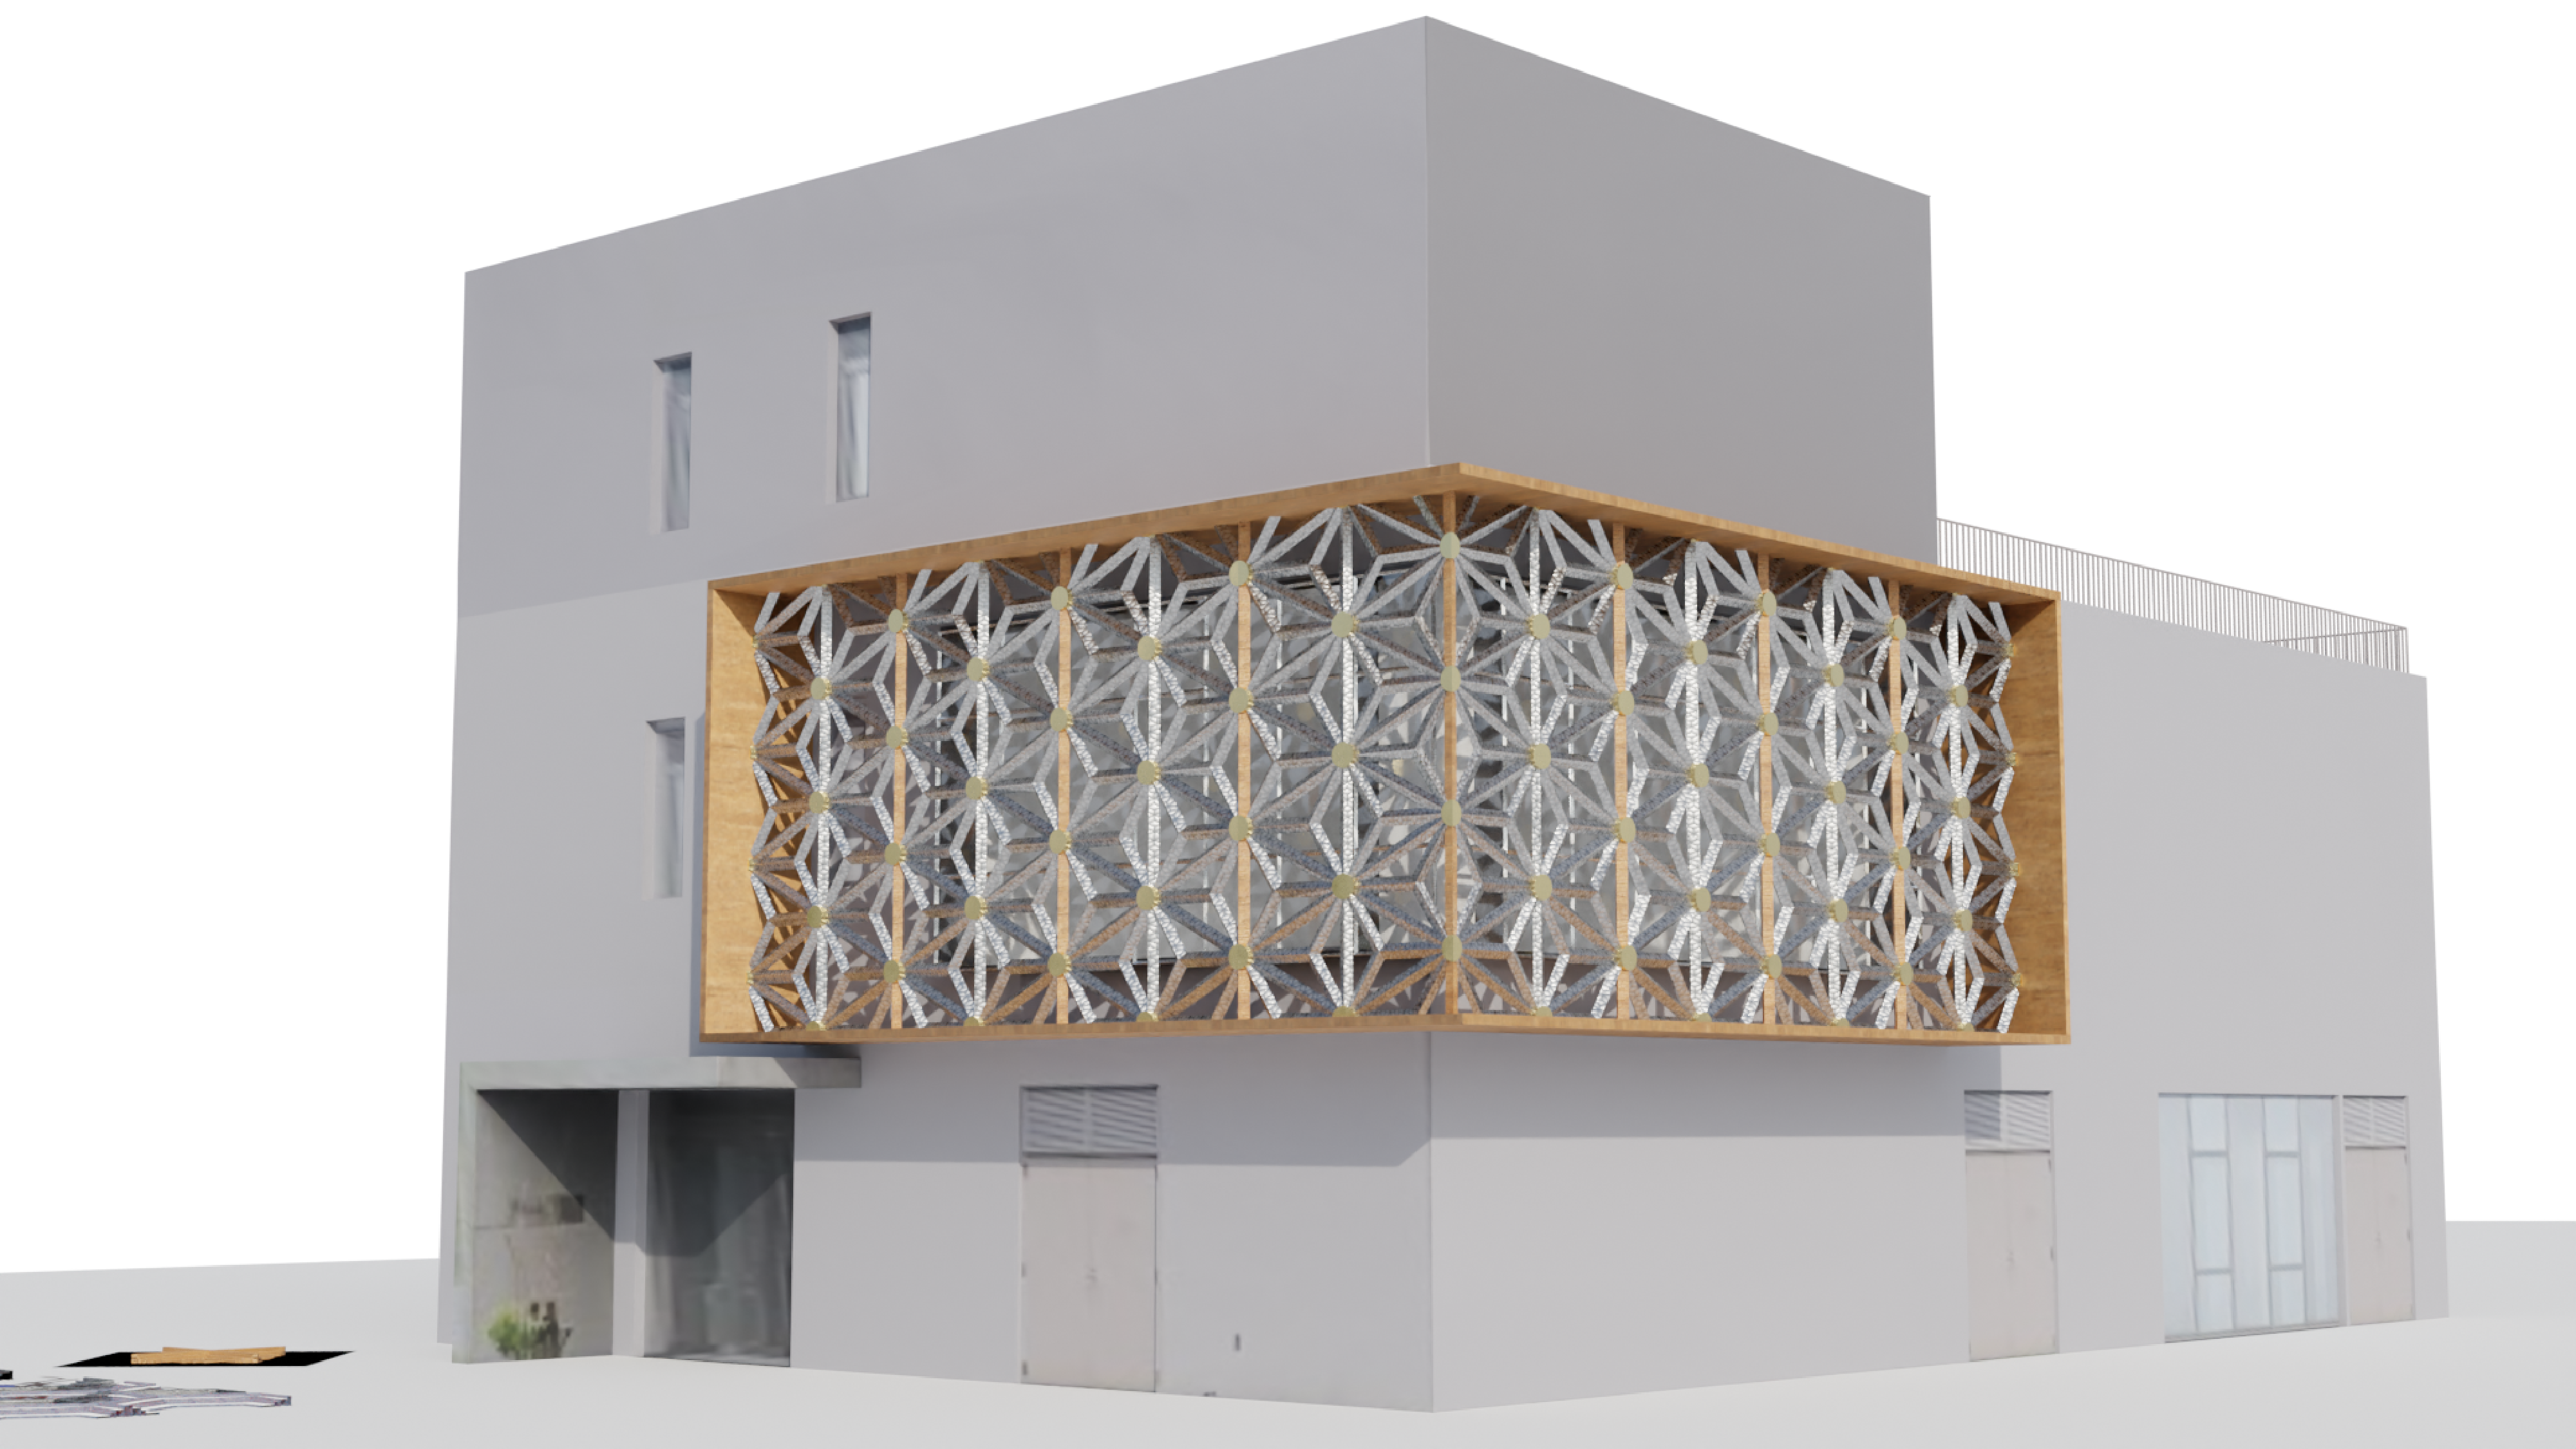
\includegraphics[width=1\linewidth]{Images/Pattern 3/0002}} \\
            \midrule
            \textit{Level 3} &  &  &
            \\
            {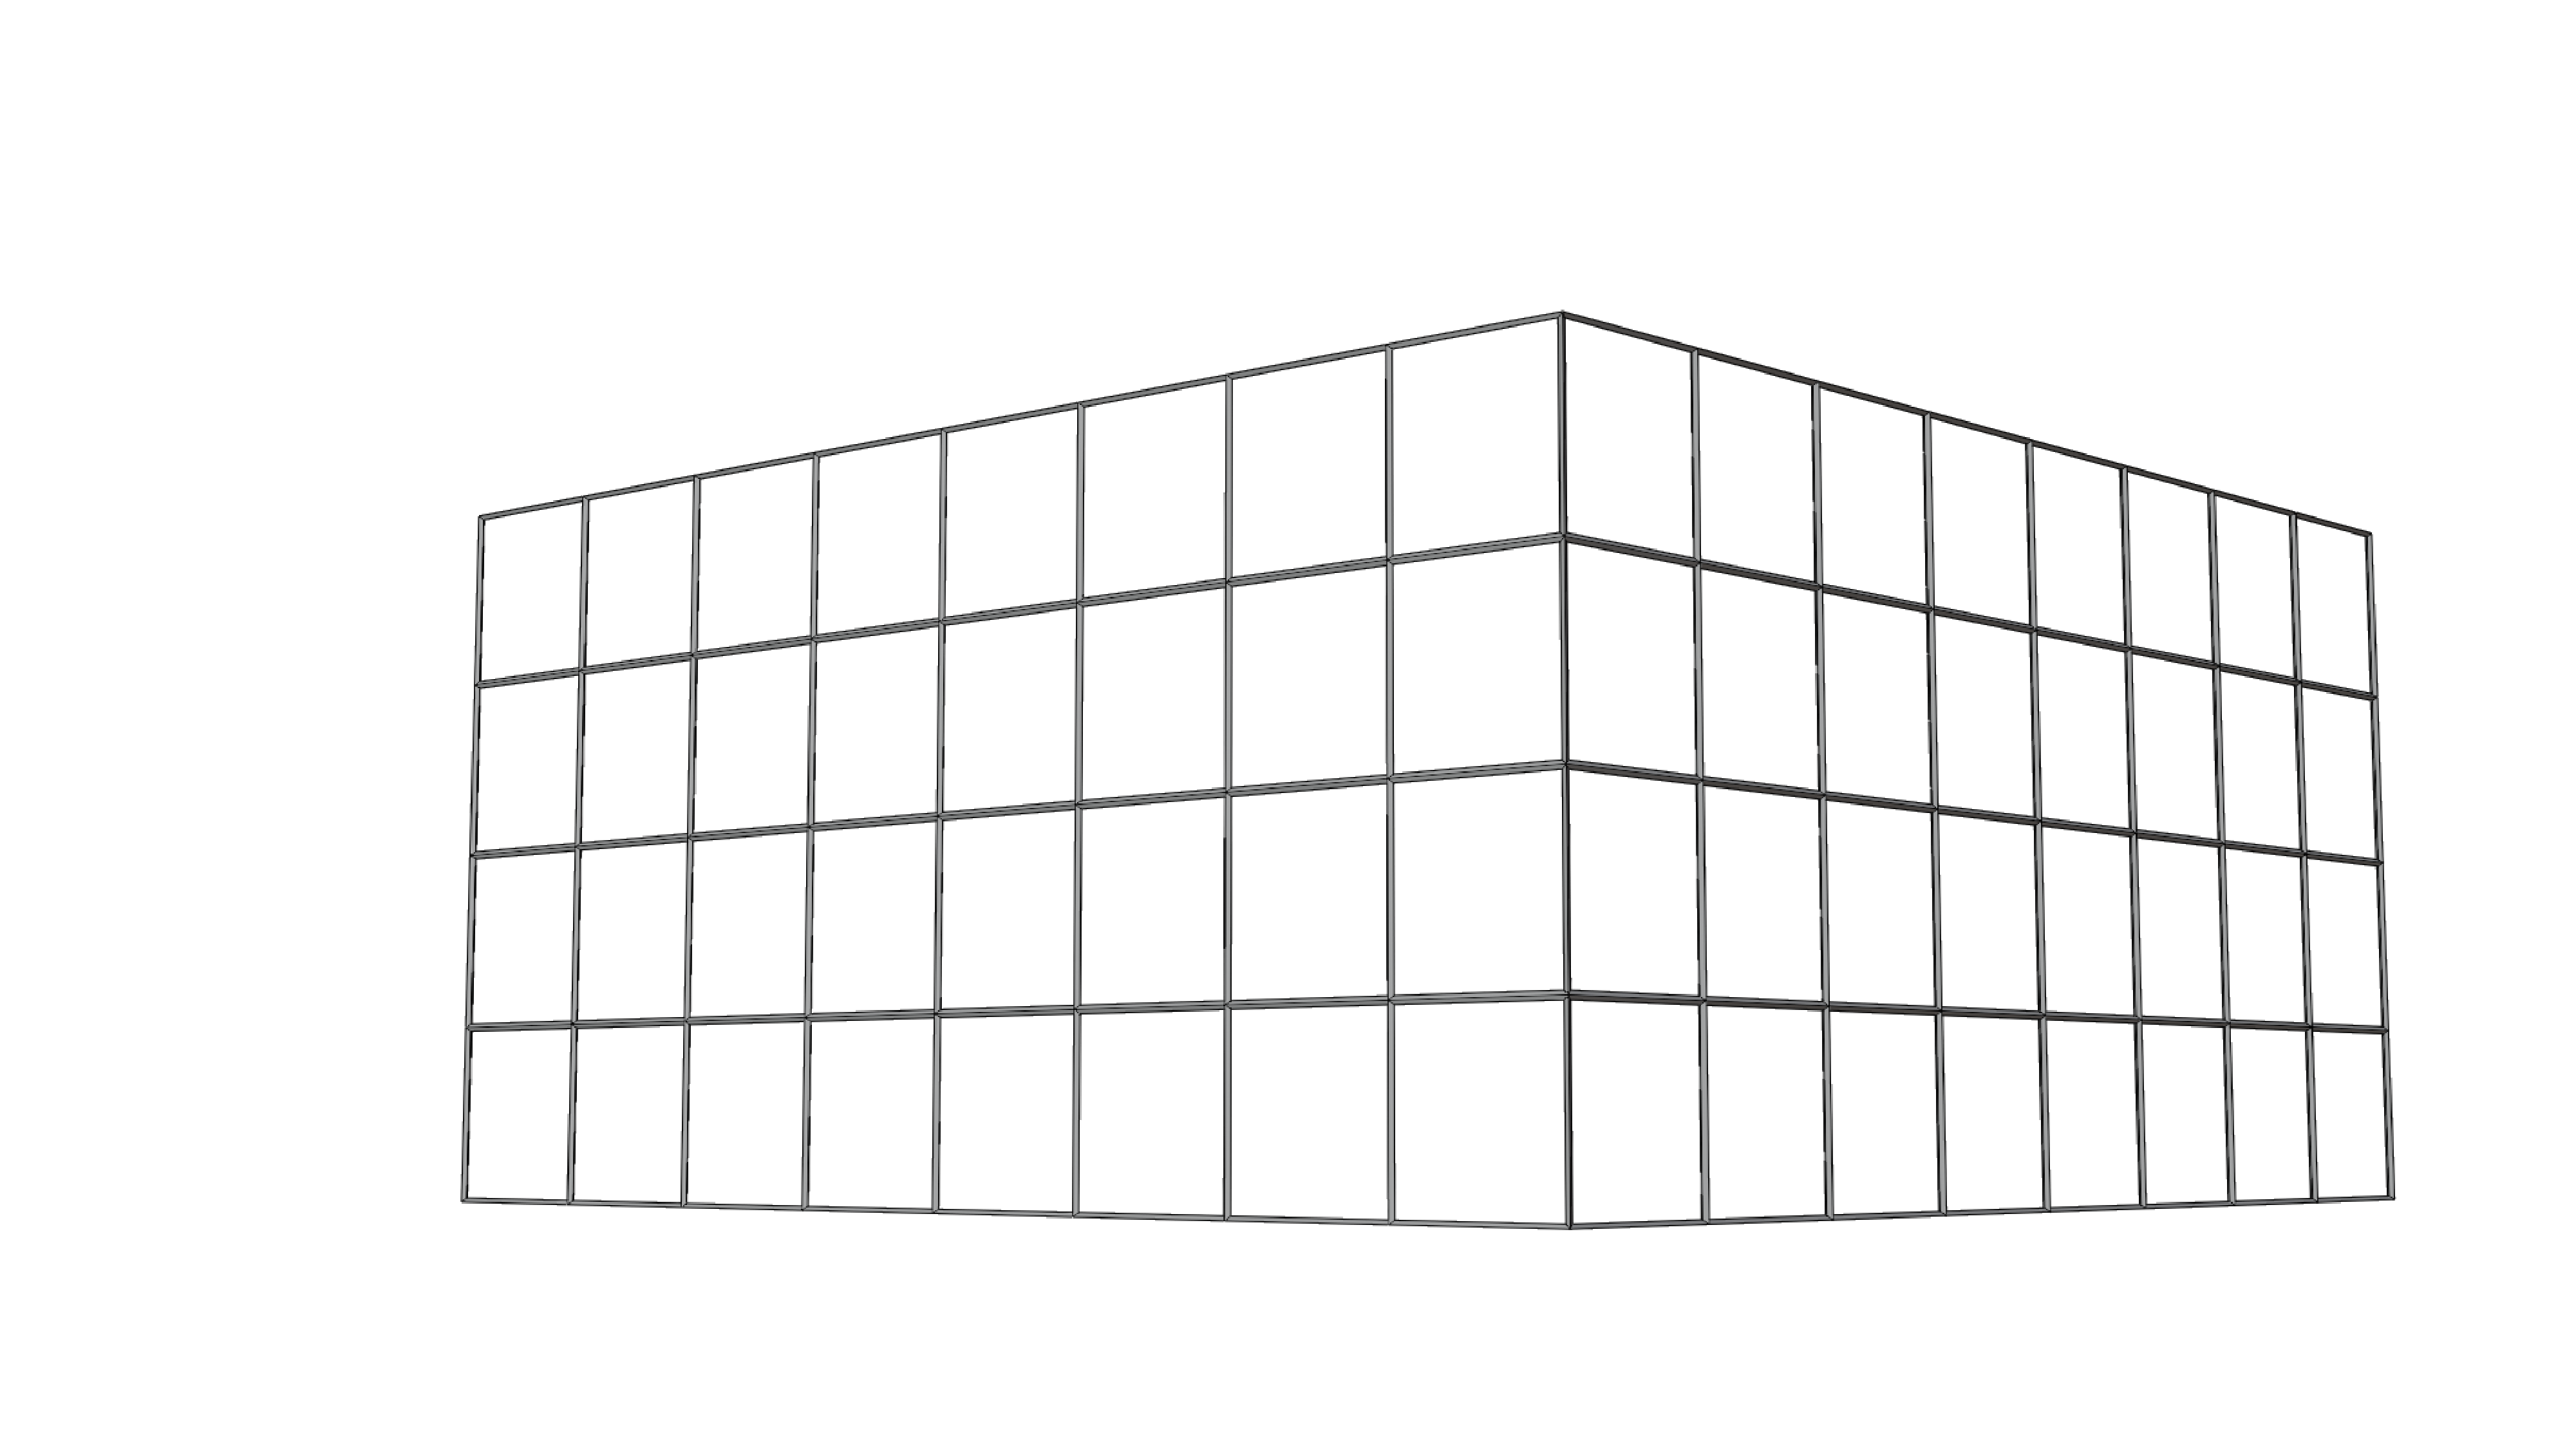
\includegraphics[width=1\linewidth]{Images/Wall 0/0003}} &
              {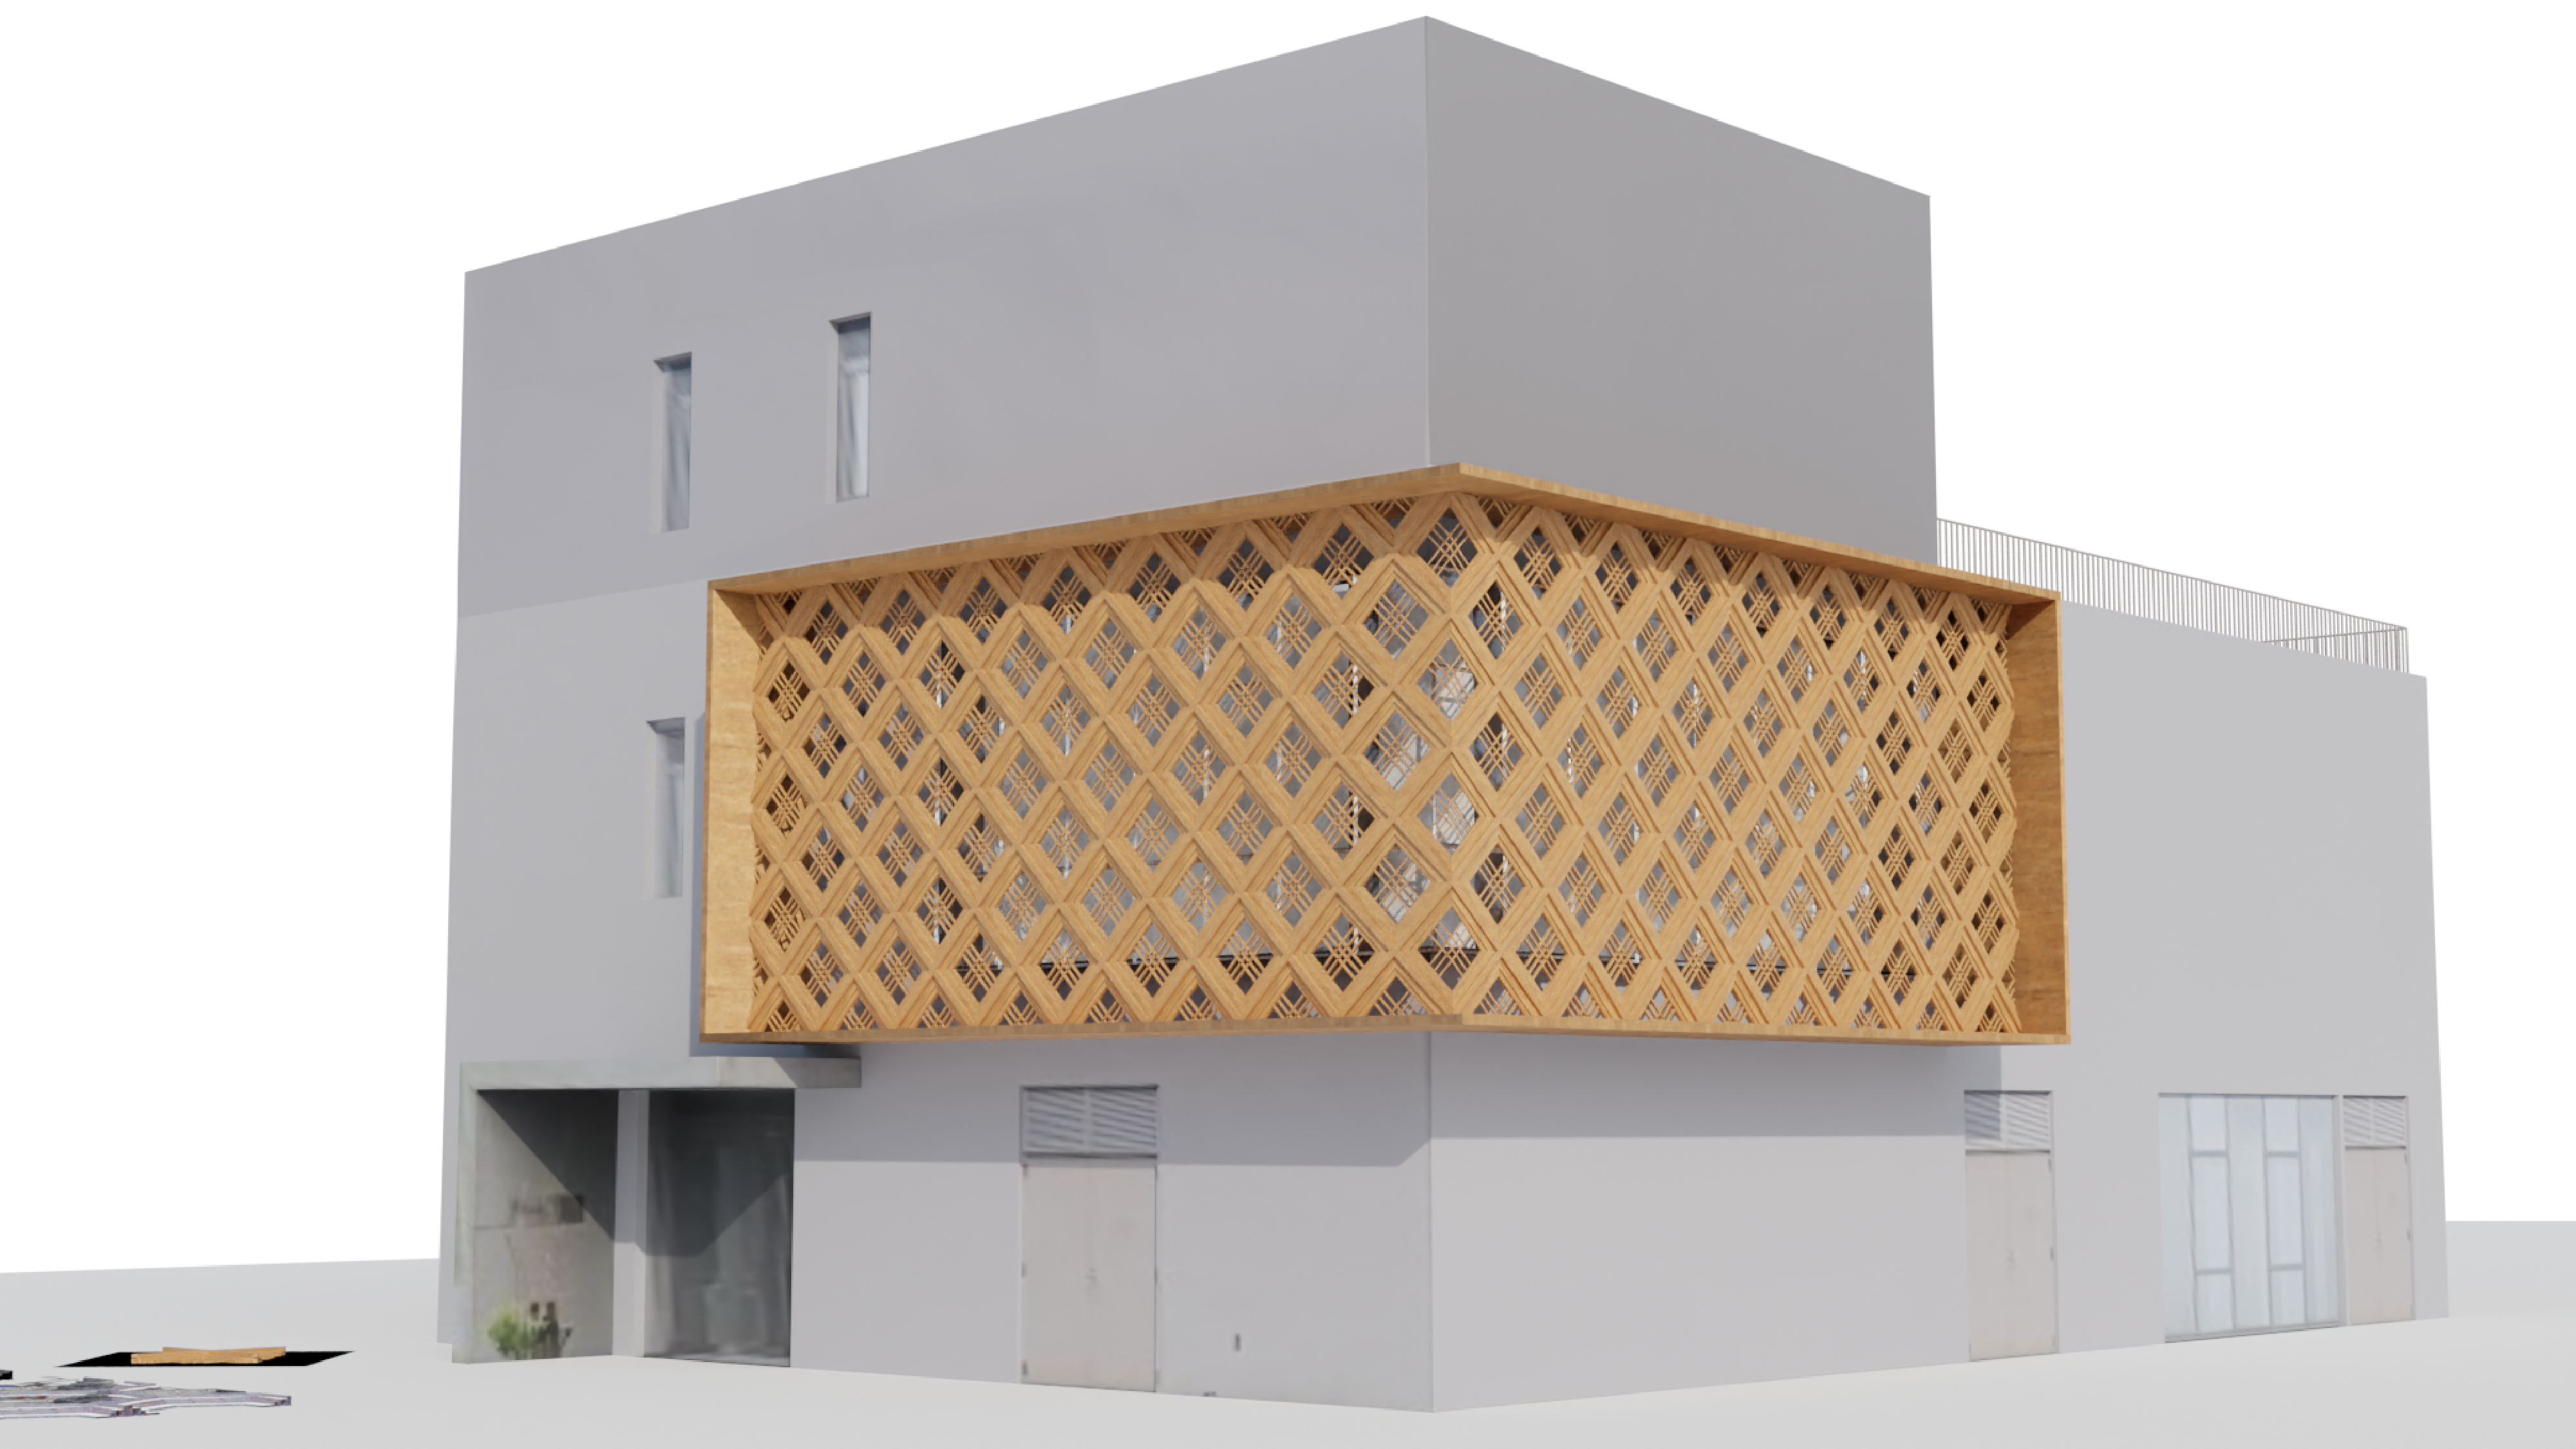
\includegraphics[width=1\linewidth]{Images/Pattern 1/0003}} &
              {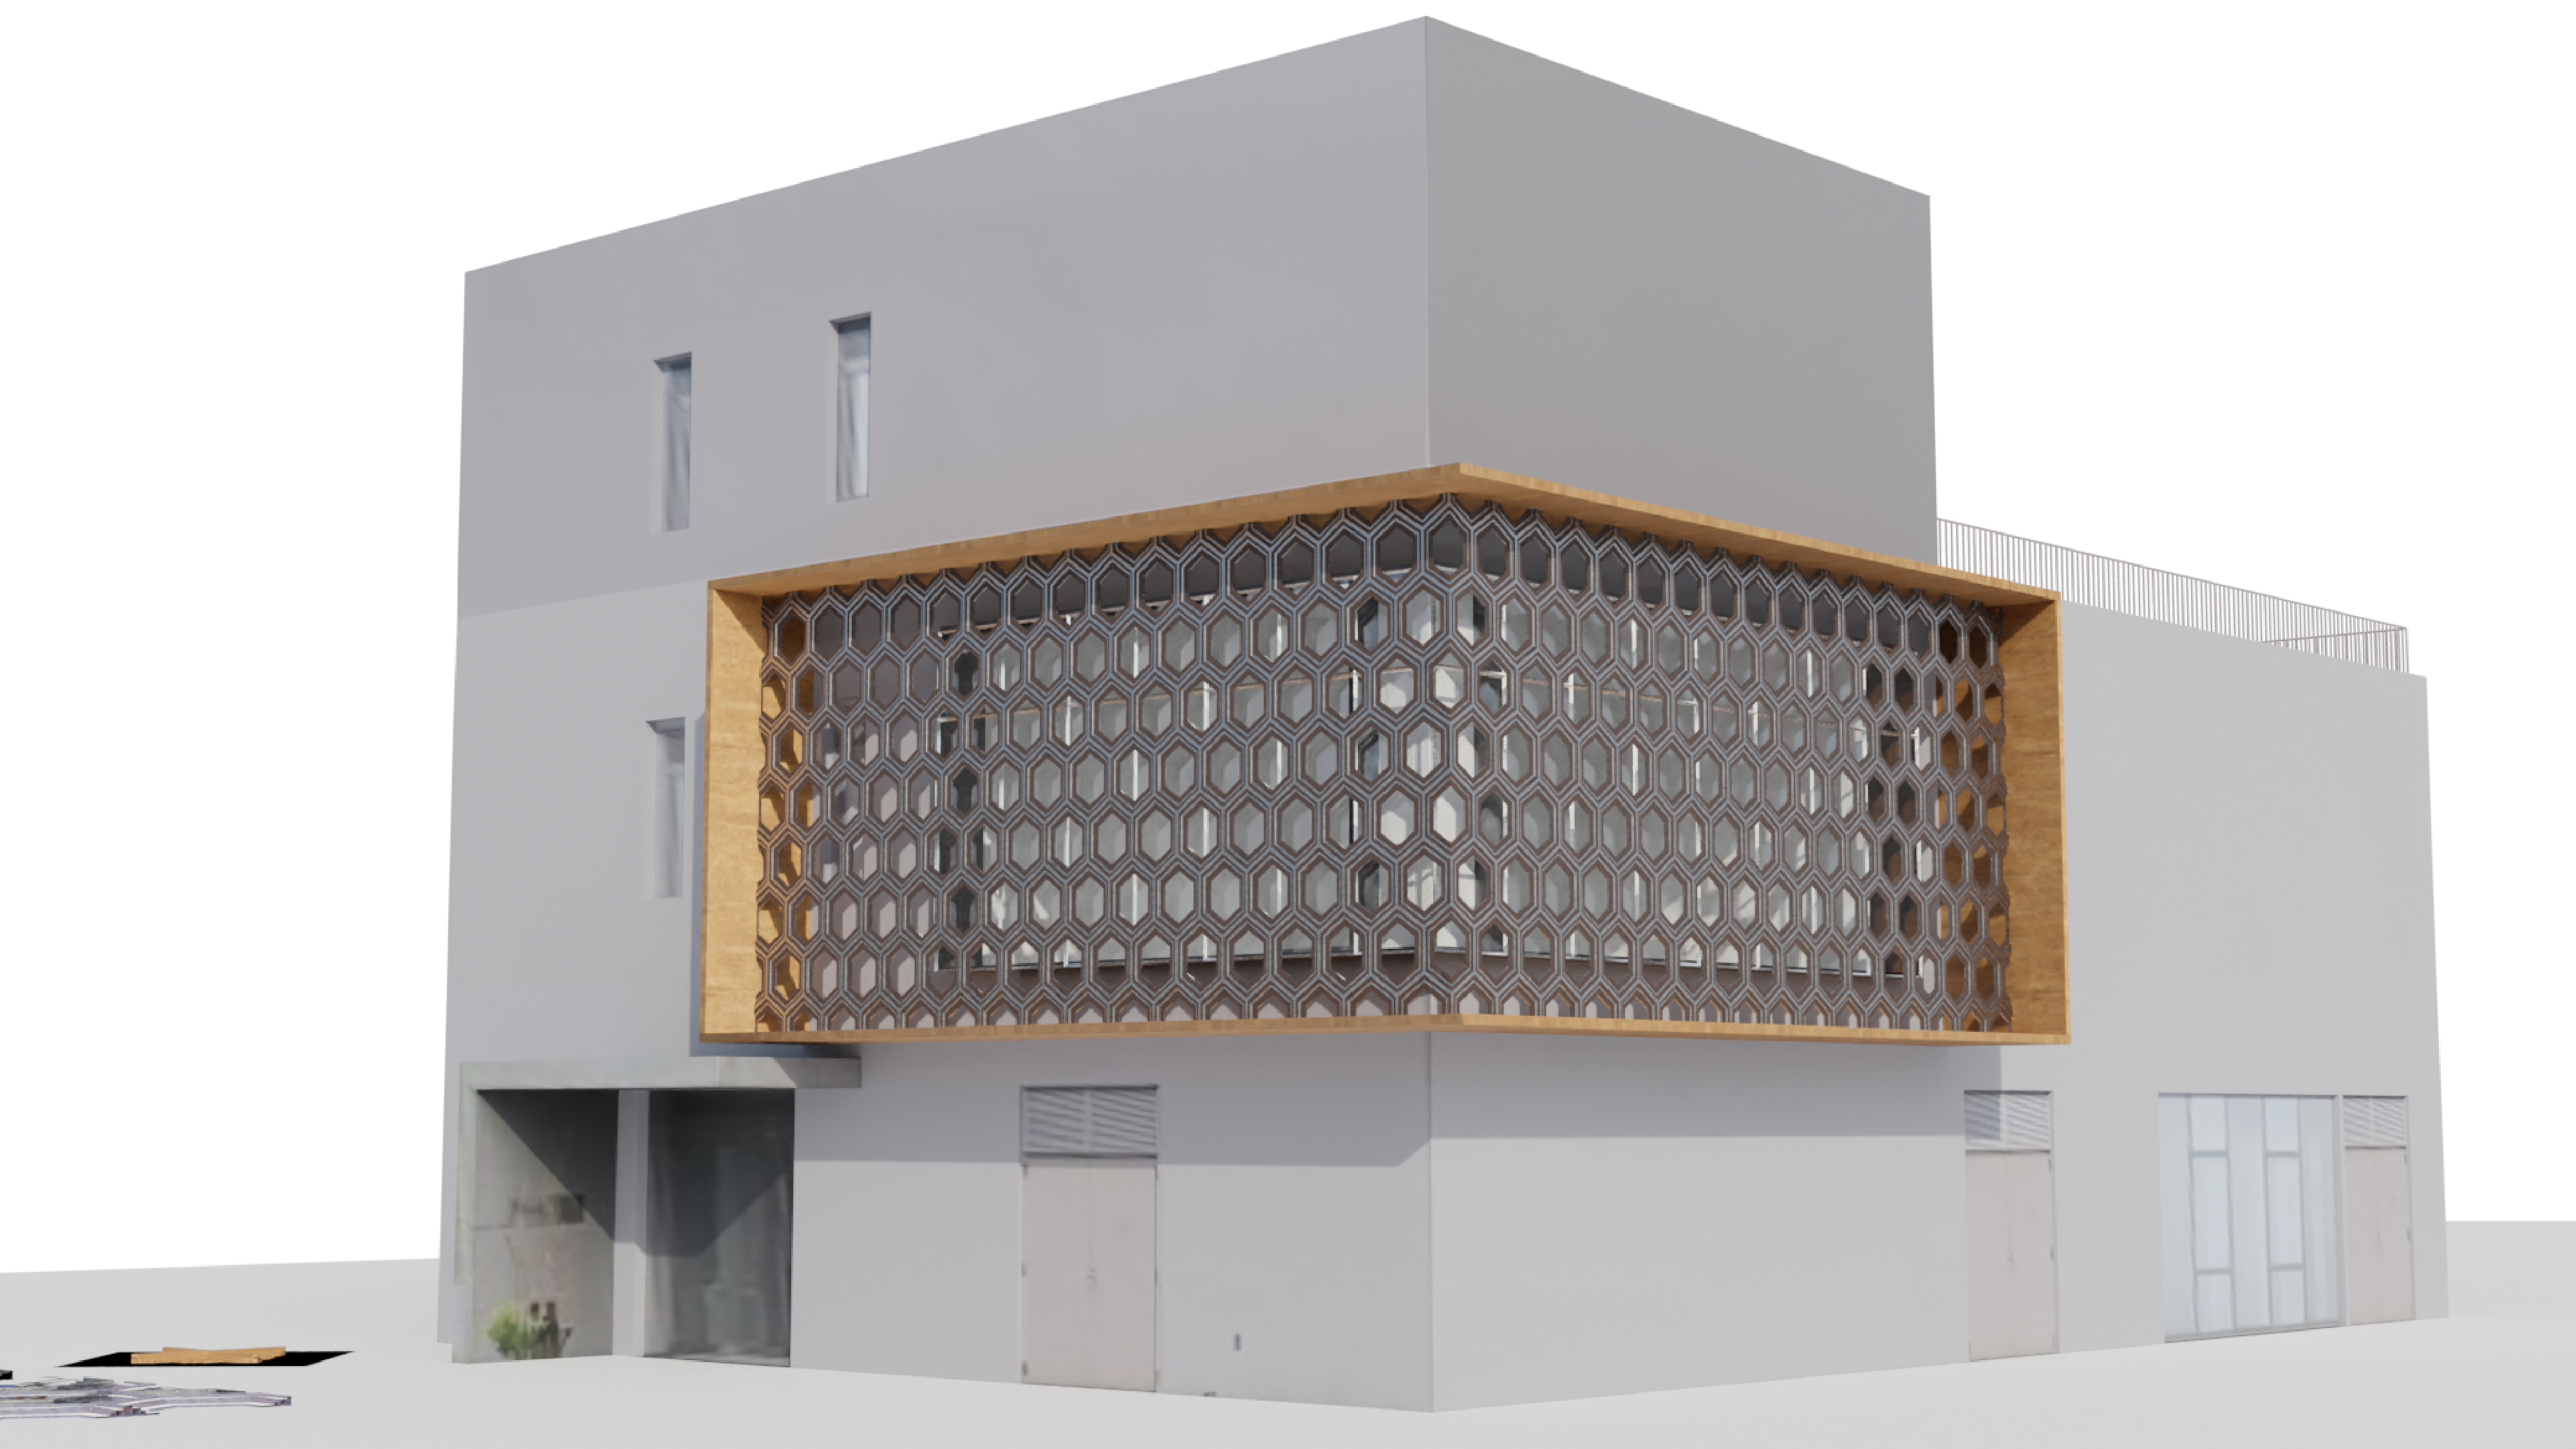
\includegraphics[width=1\linewidth]{Images/Pattern 2/0003}} &
              {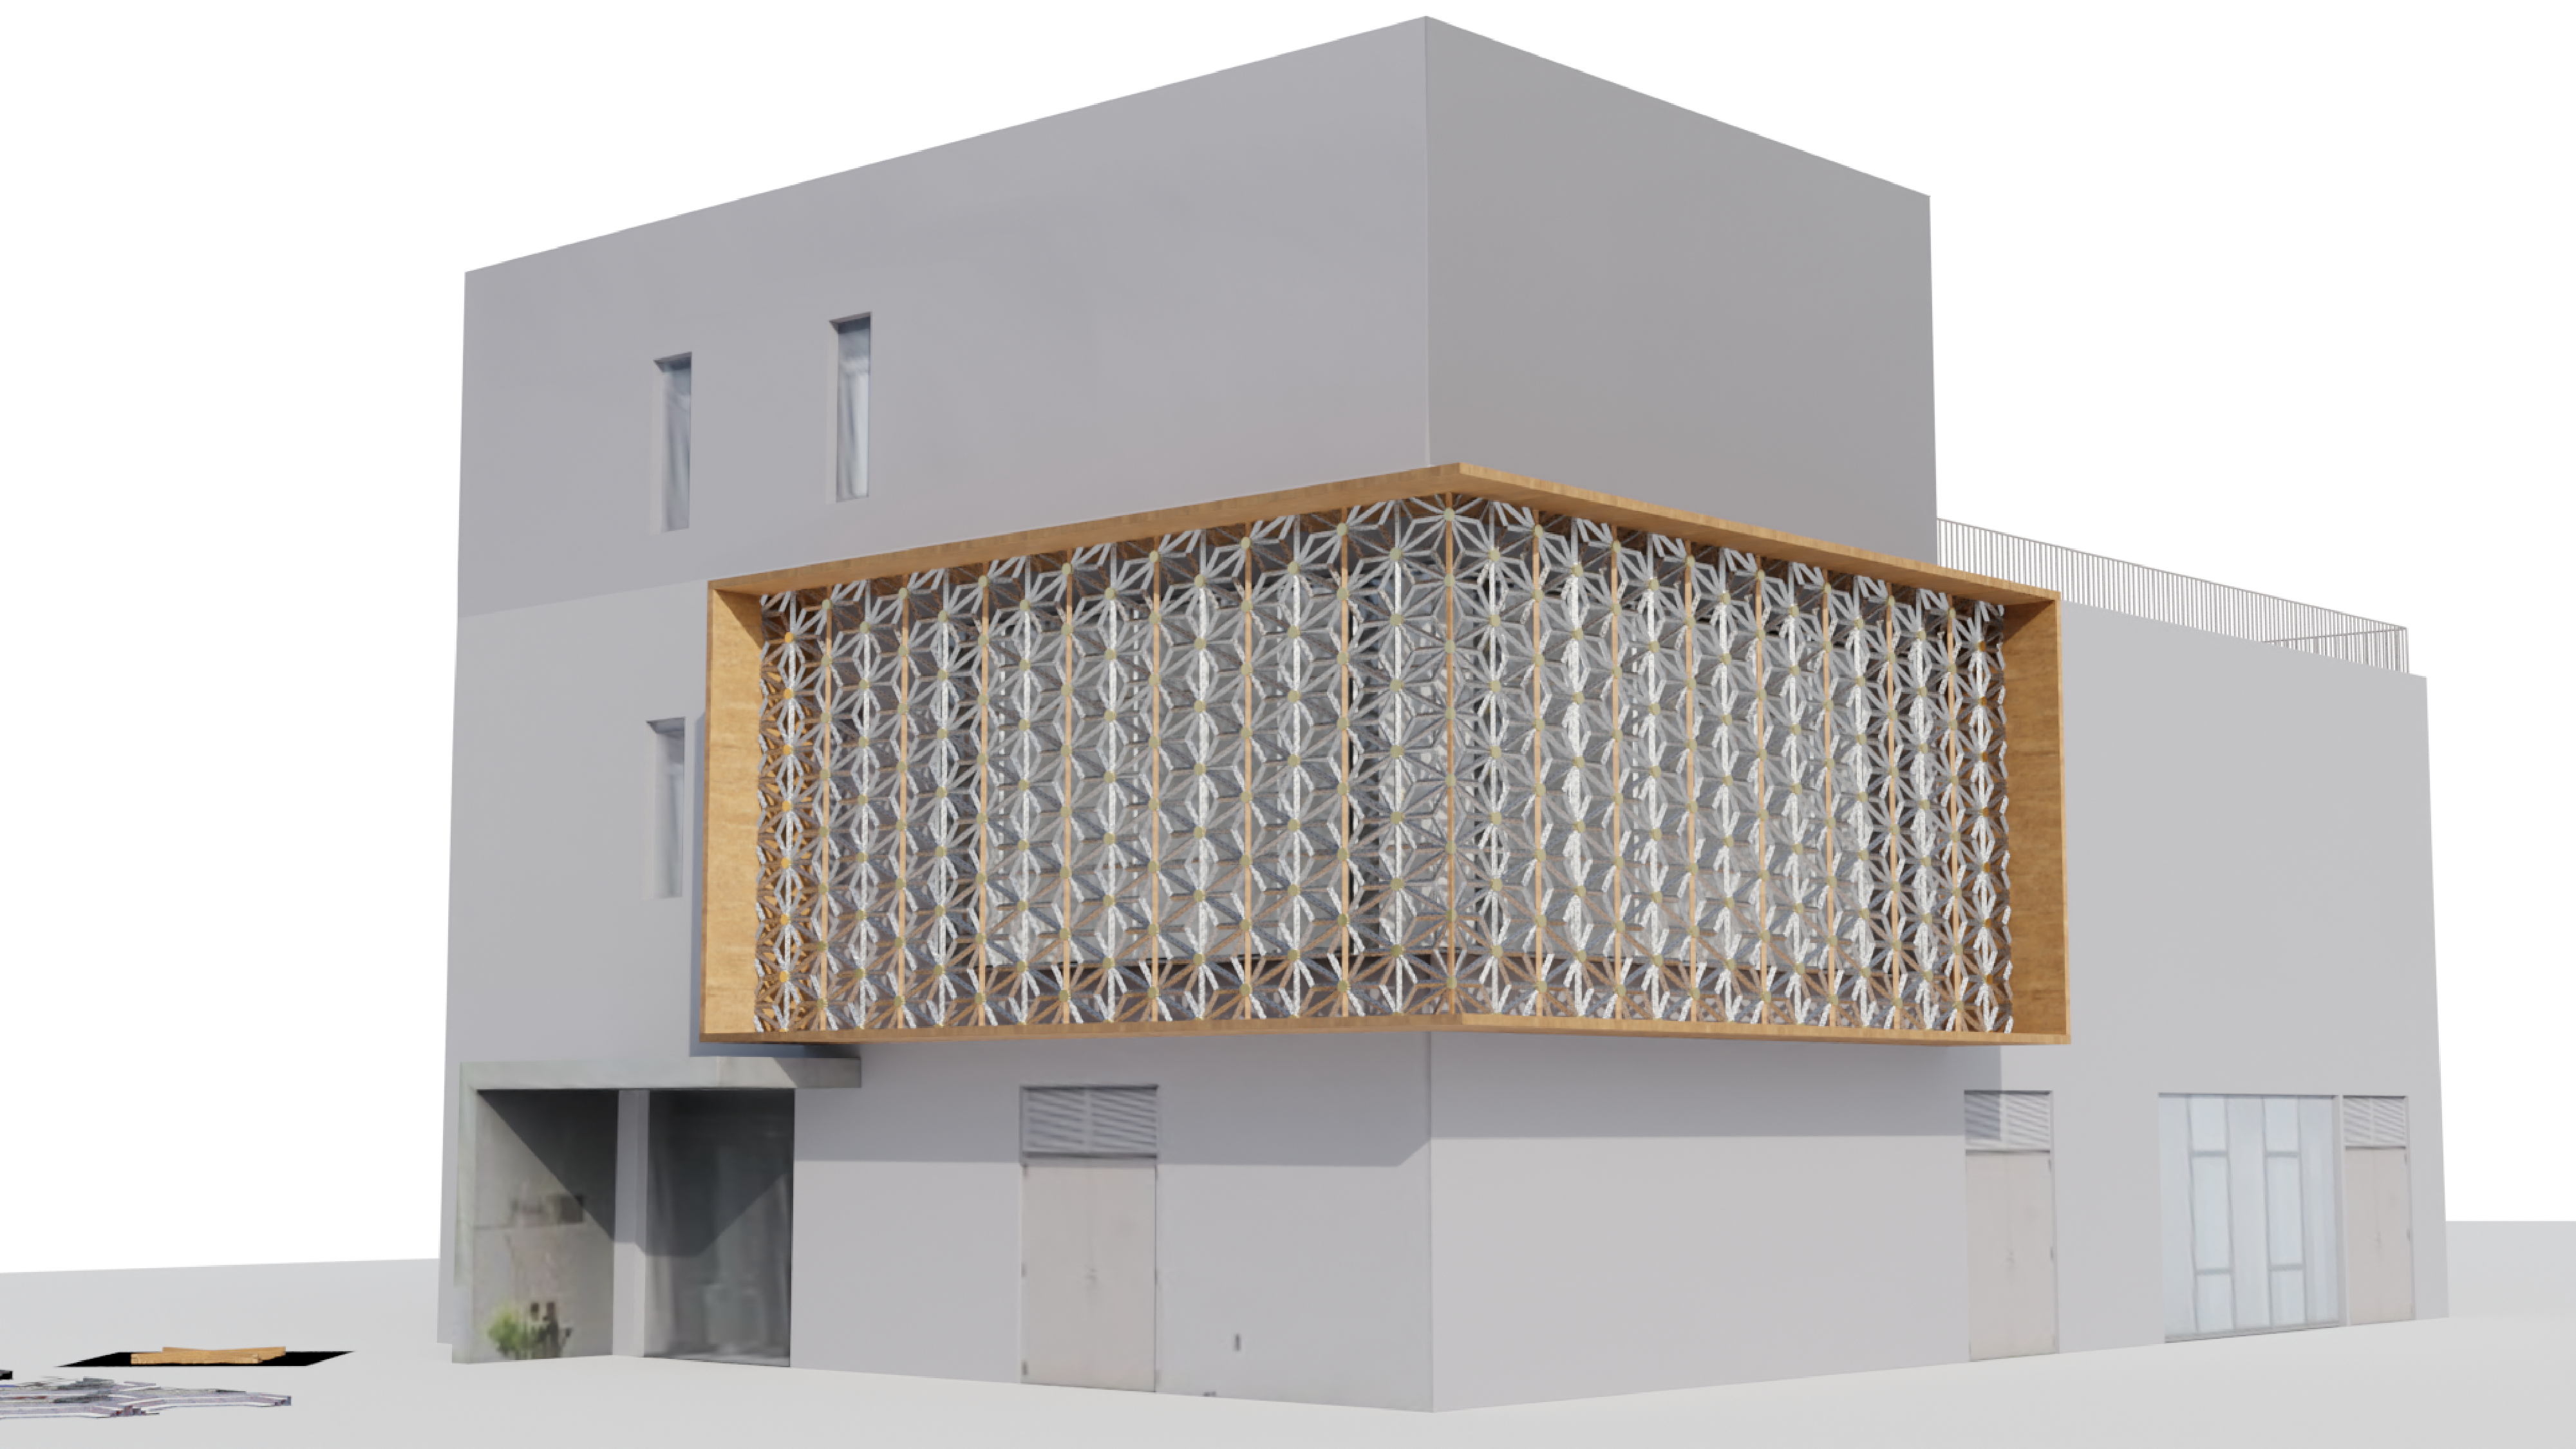
\includegraphics[width=1\linewidth]{Images/Pattern 3/0003}} \\
            \midrule
            \textit{Level 4} &  &  &
            \\
            {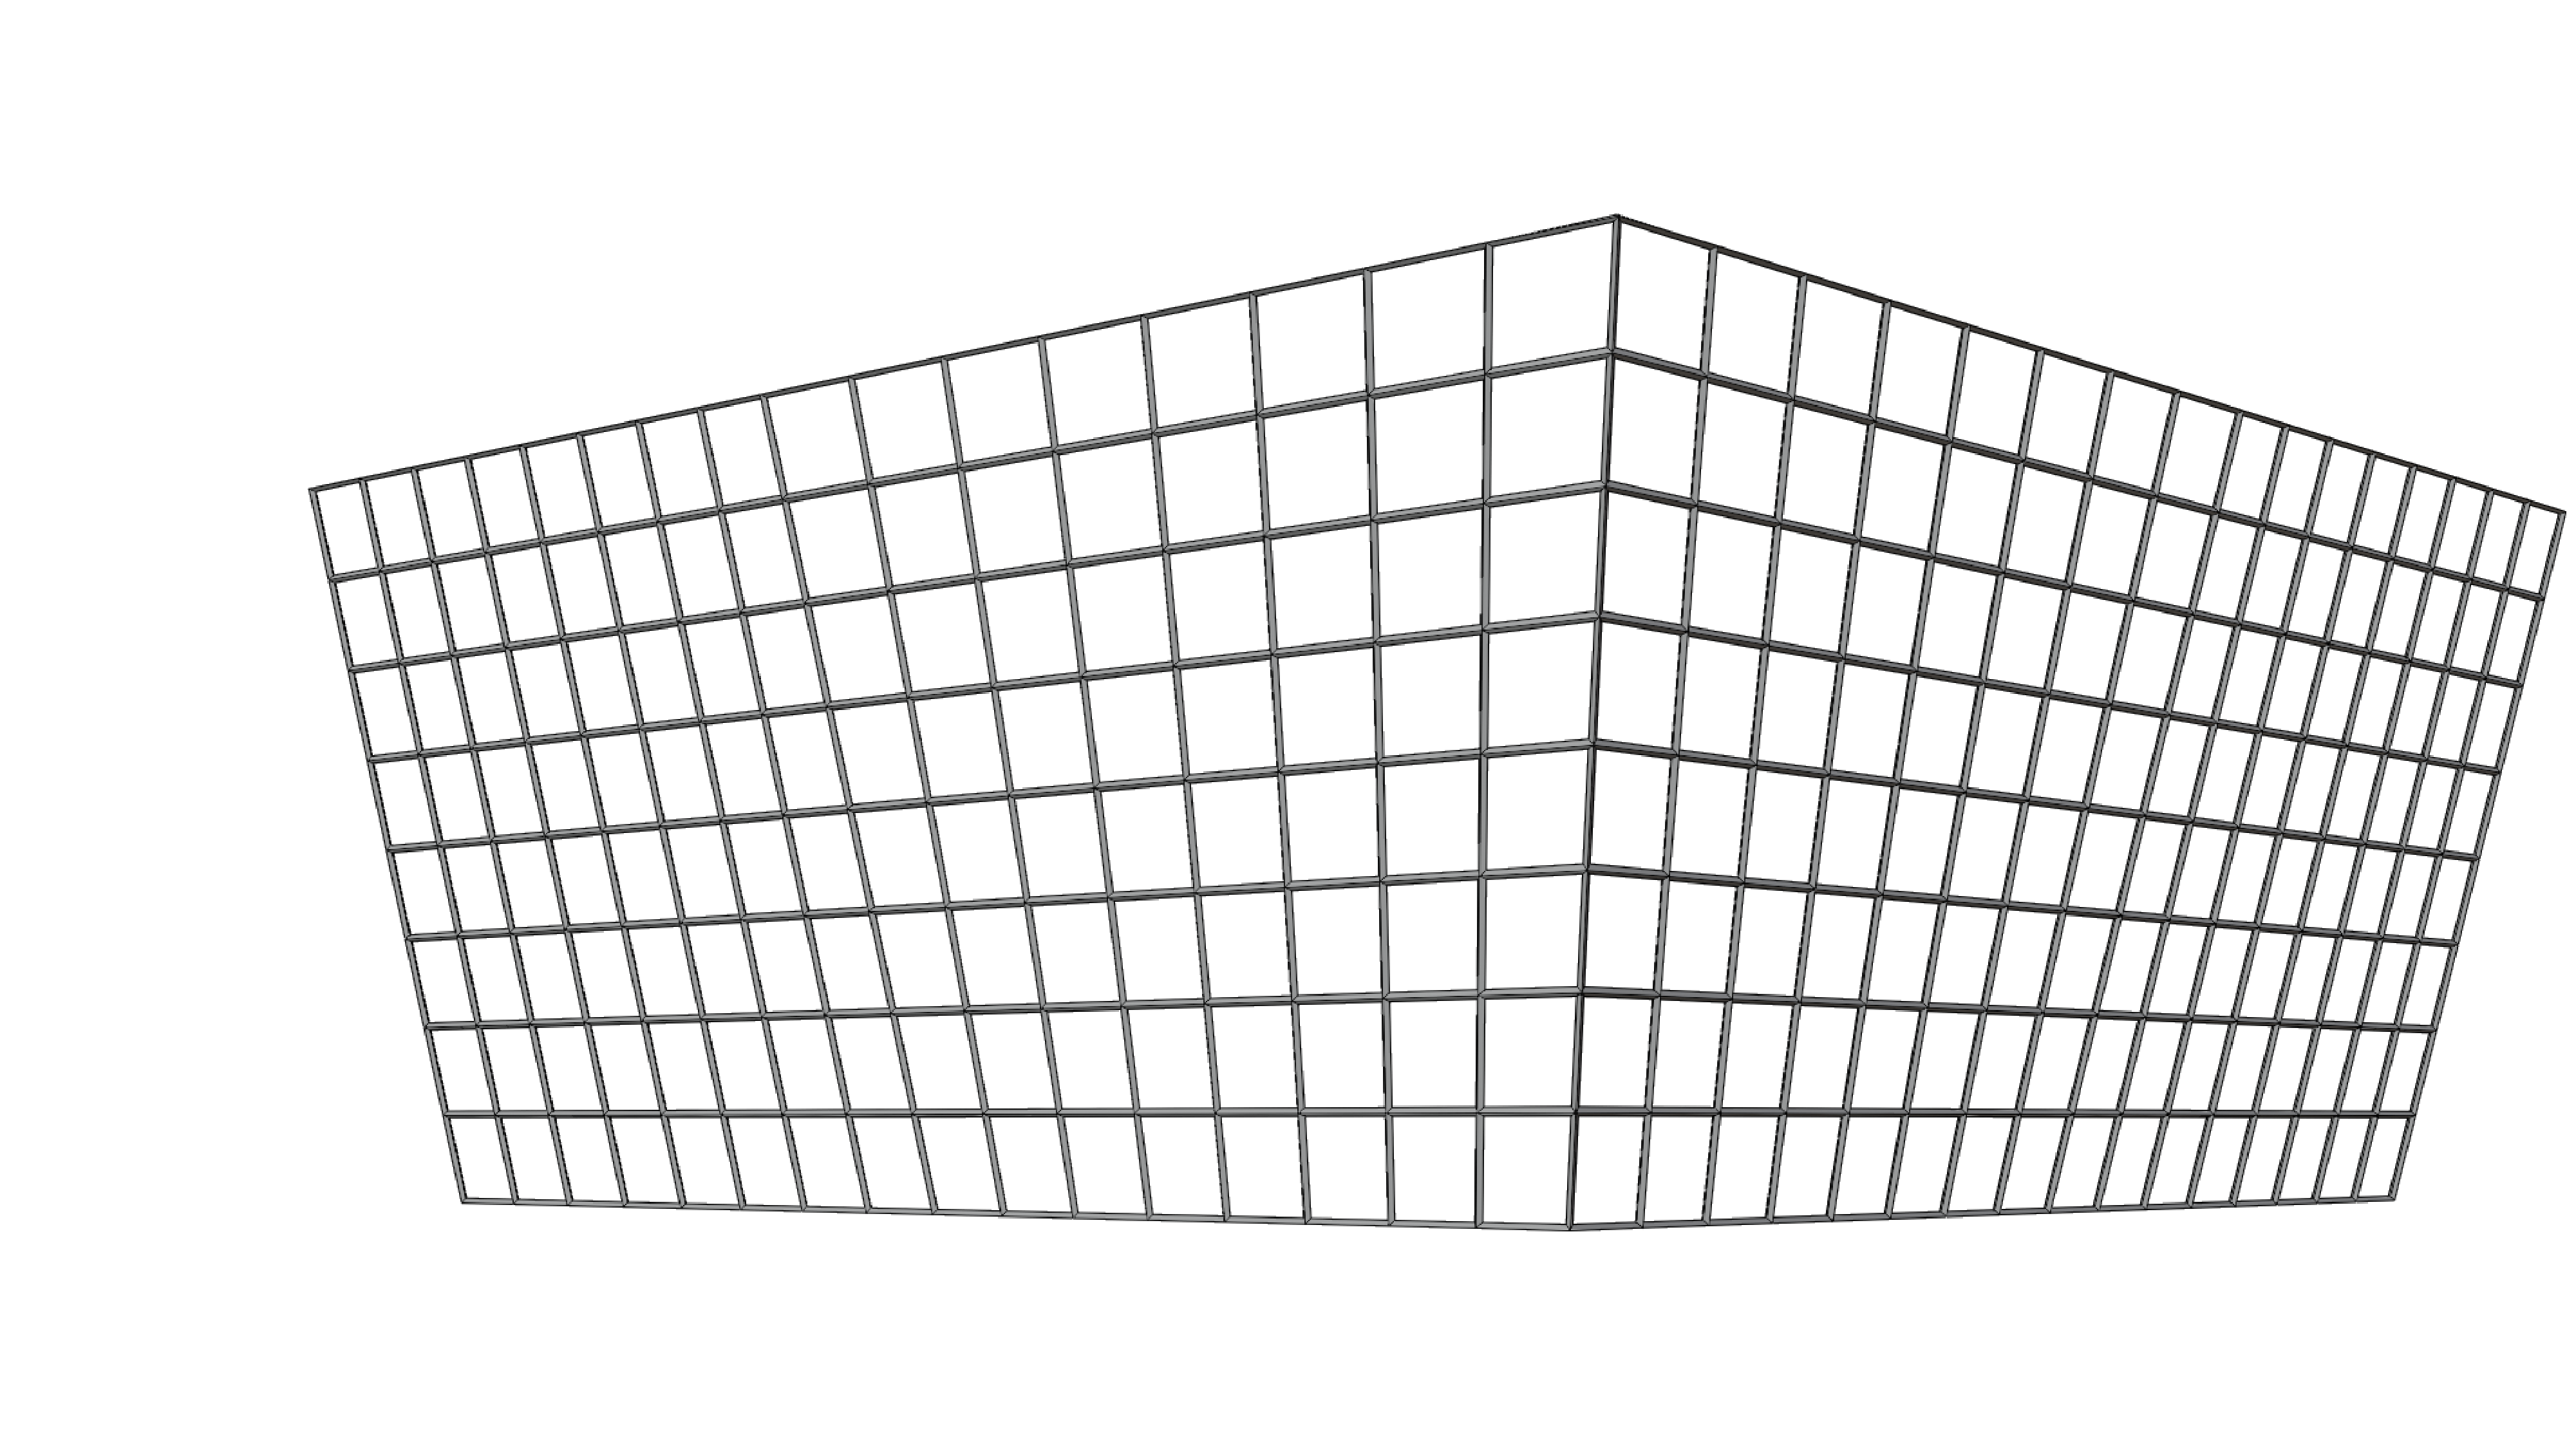
\includegraphics[width=1\linewidth]{Images/Wall 0/0004}} &
              {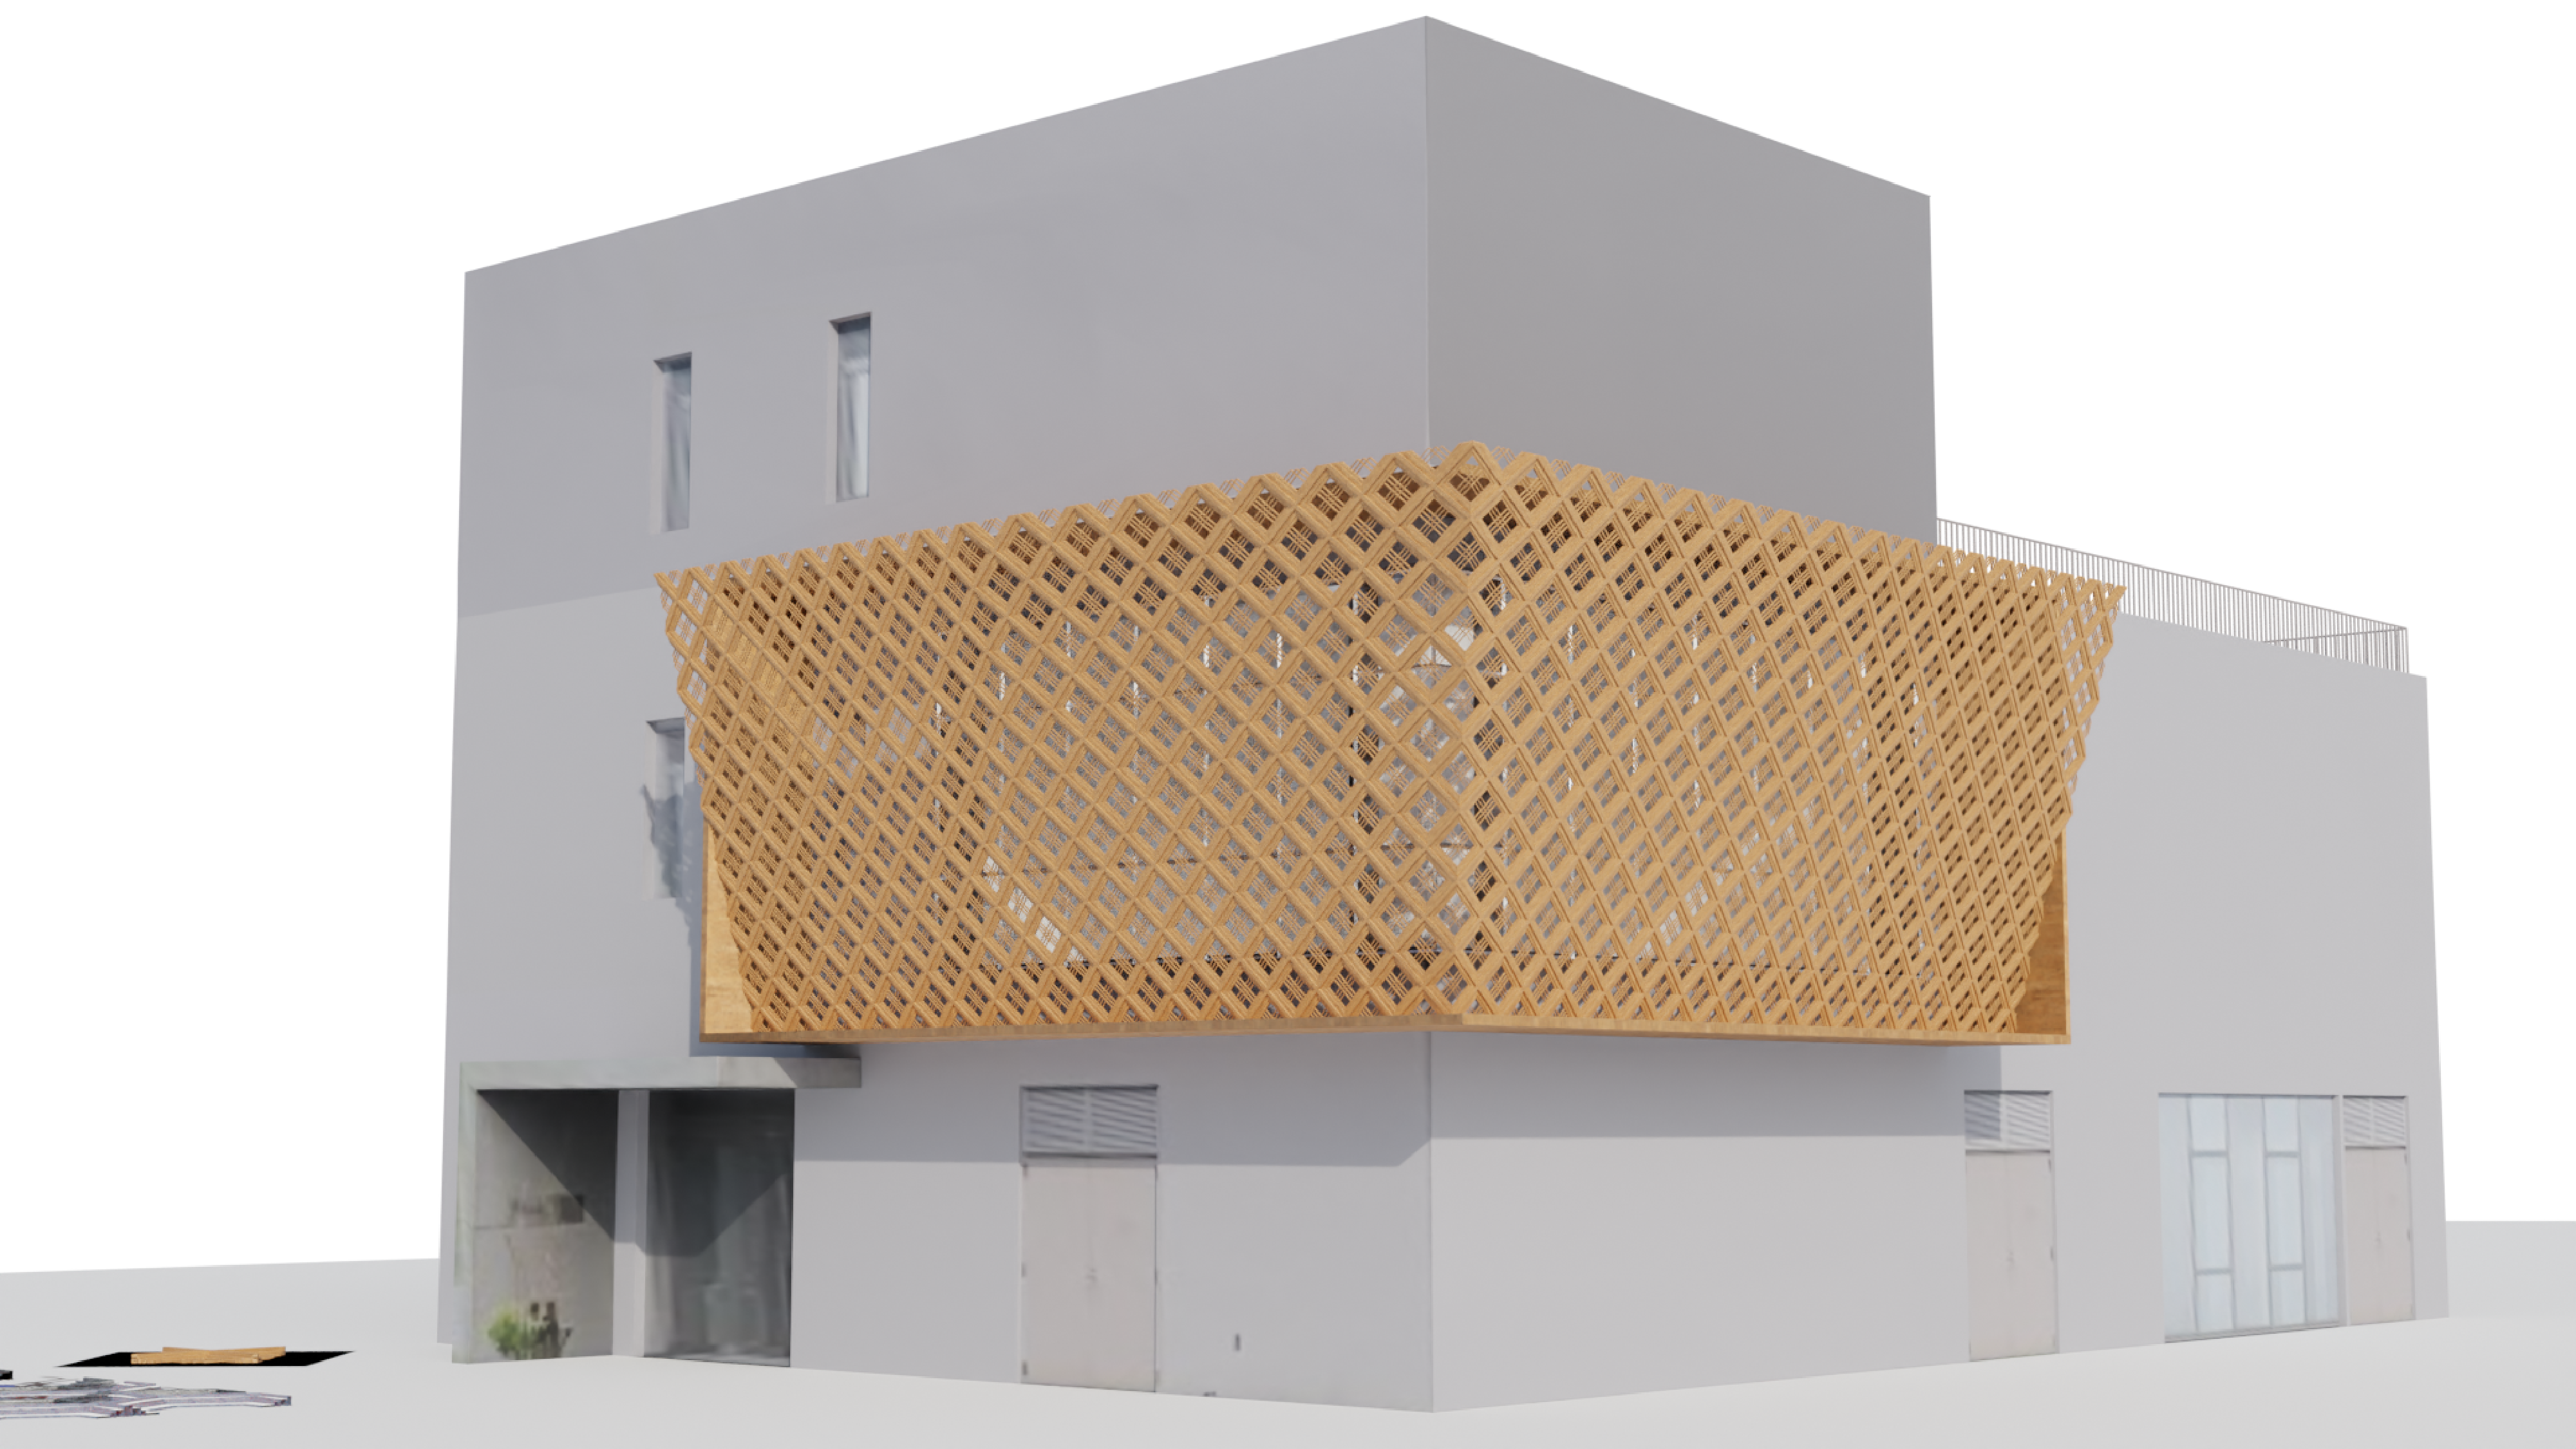
\includegraphics[width=1\linewidth]{Images/Pattern 1/0004}} &
              {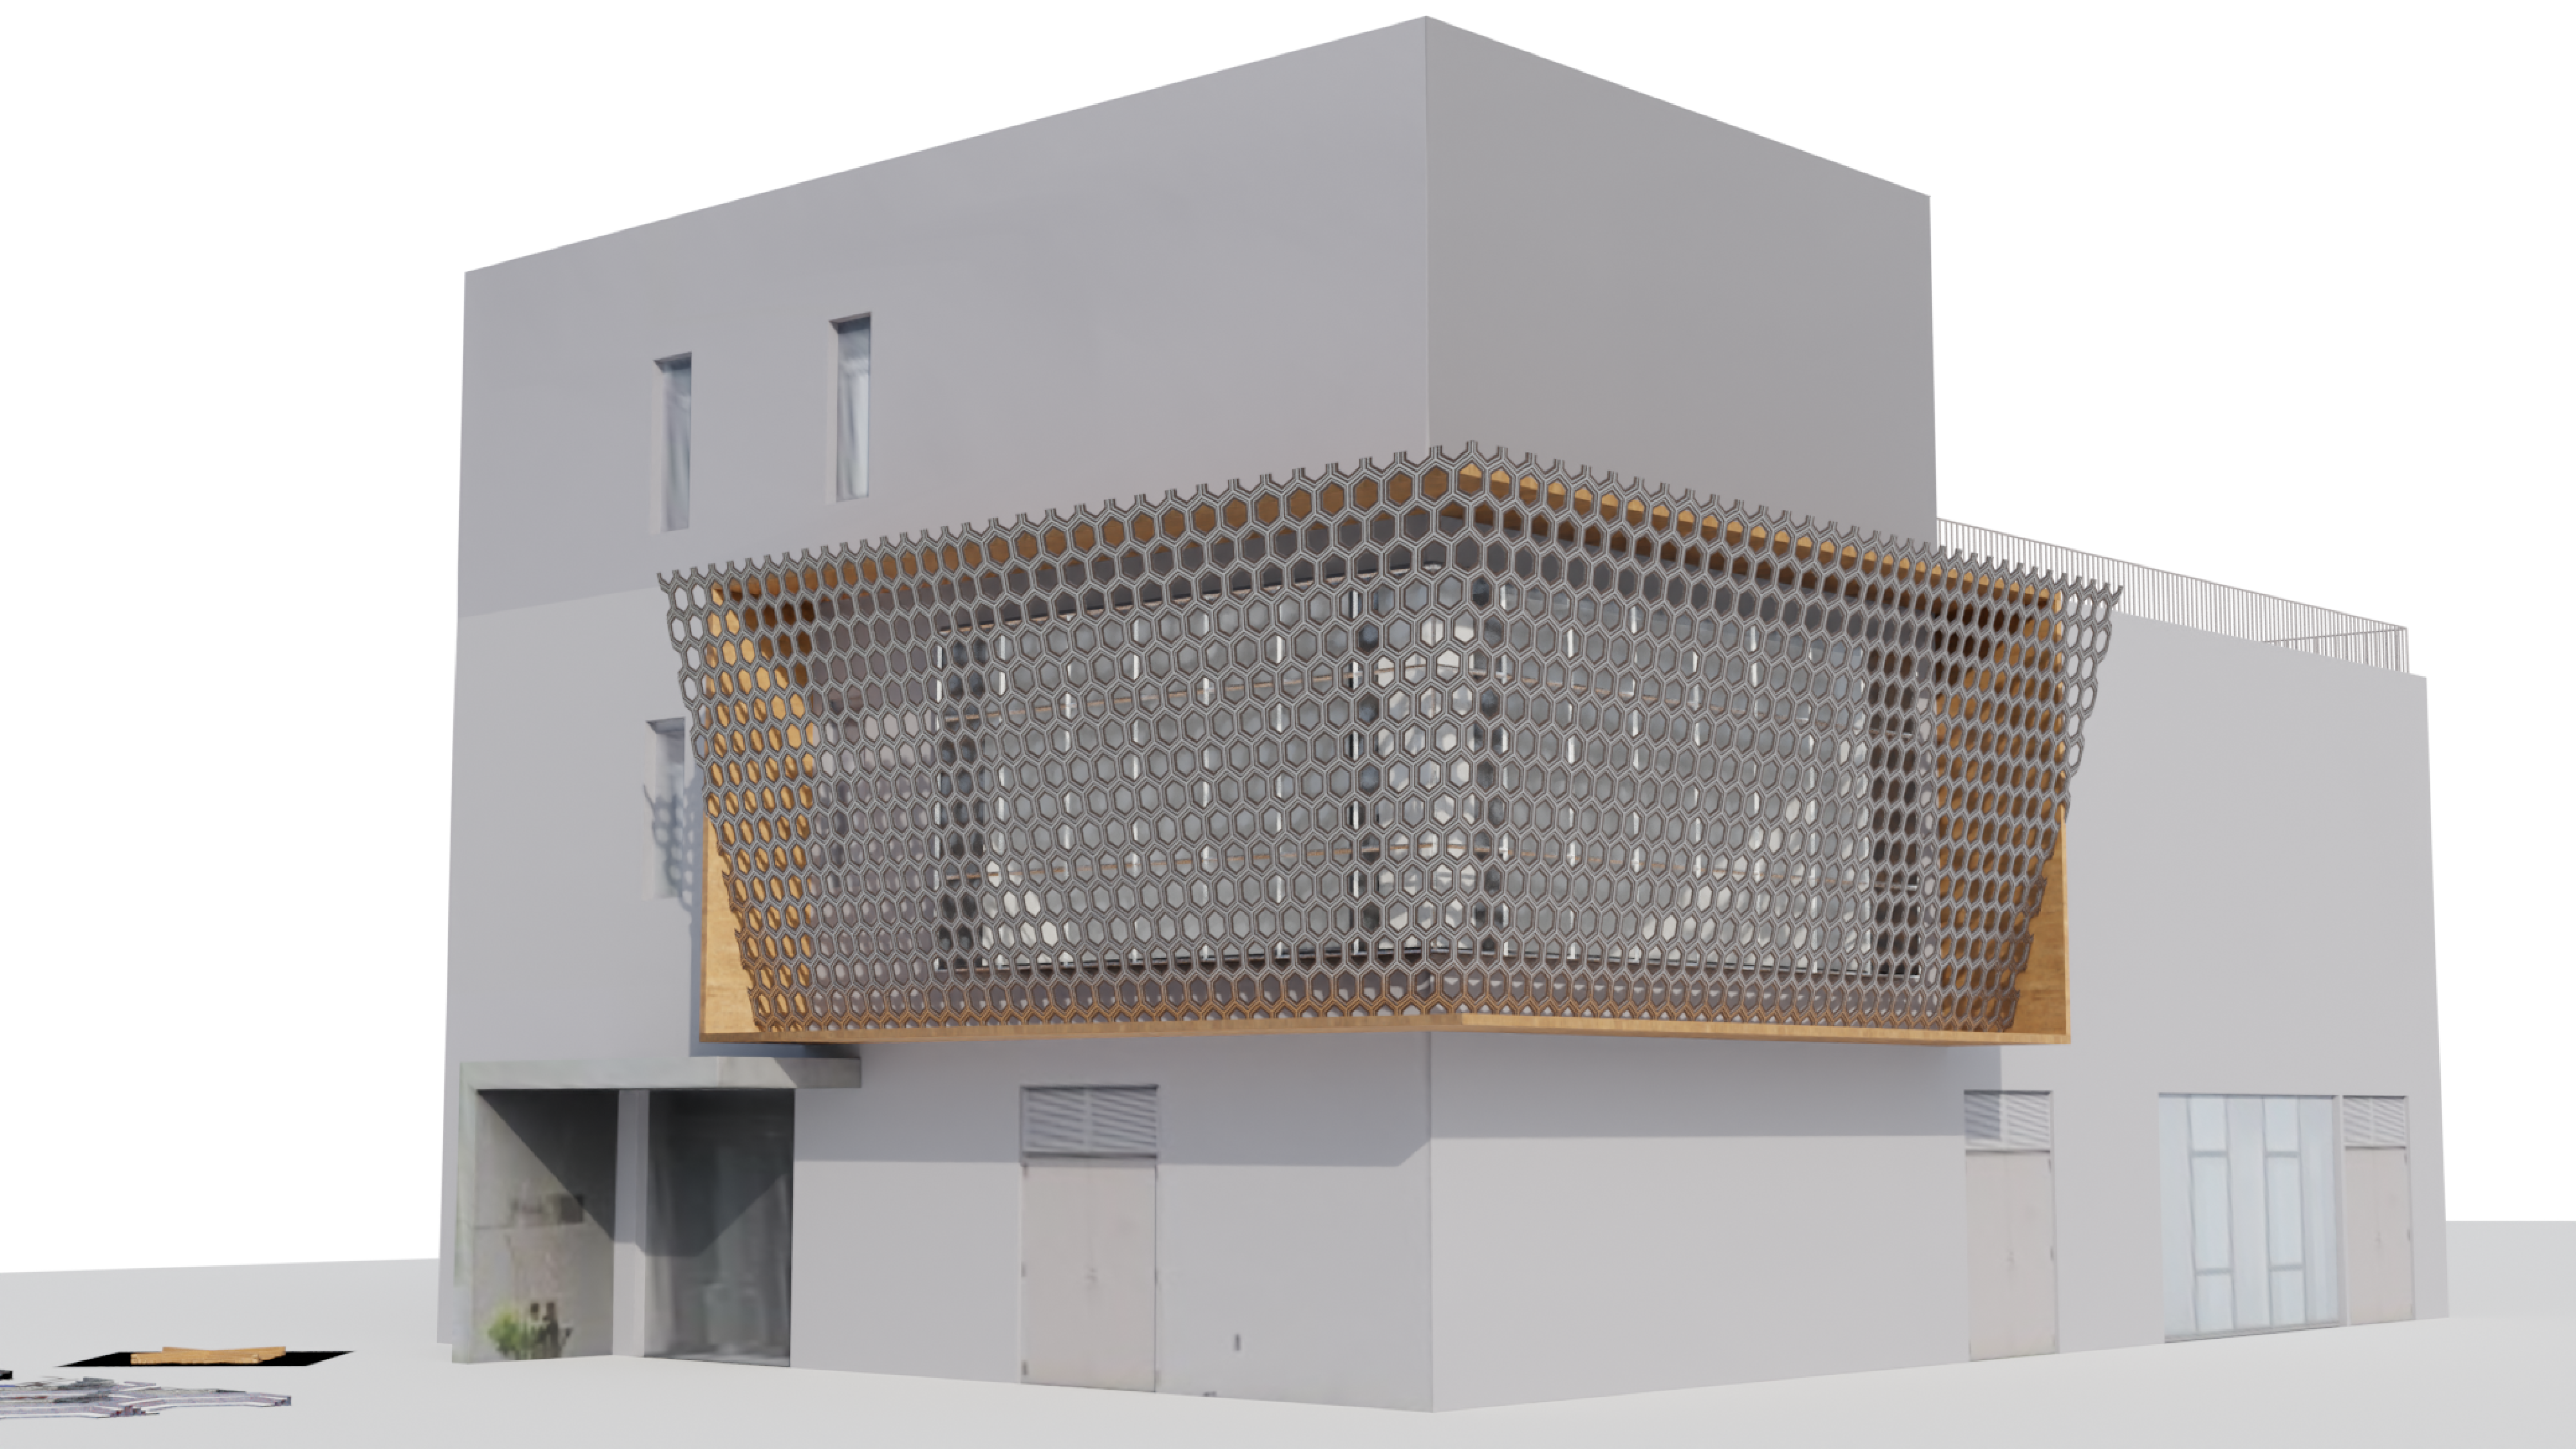
\includegraphics[width=1\linewidth]{Images/Pattern 2/0004}} &
              {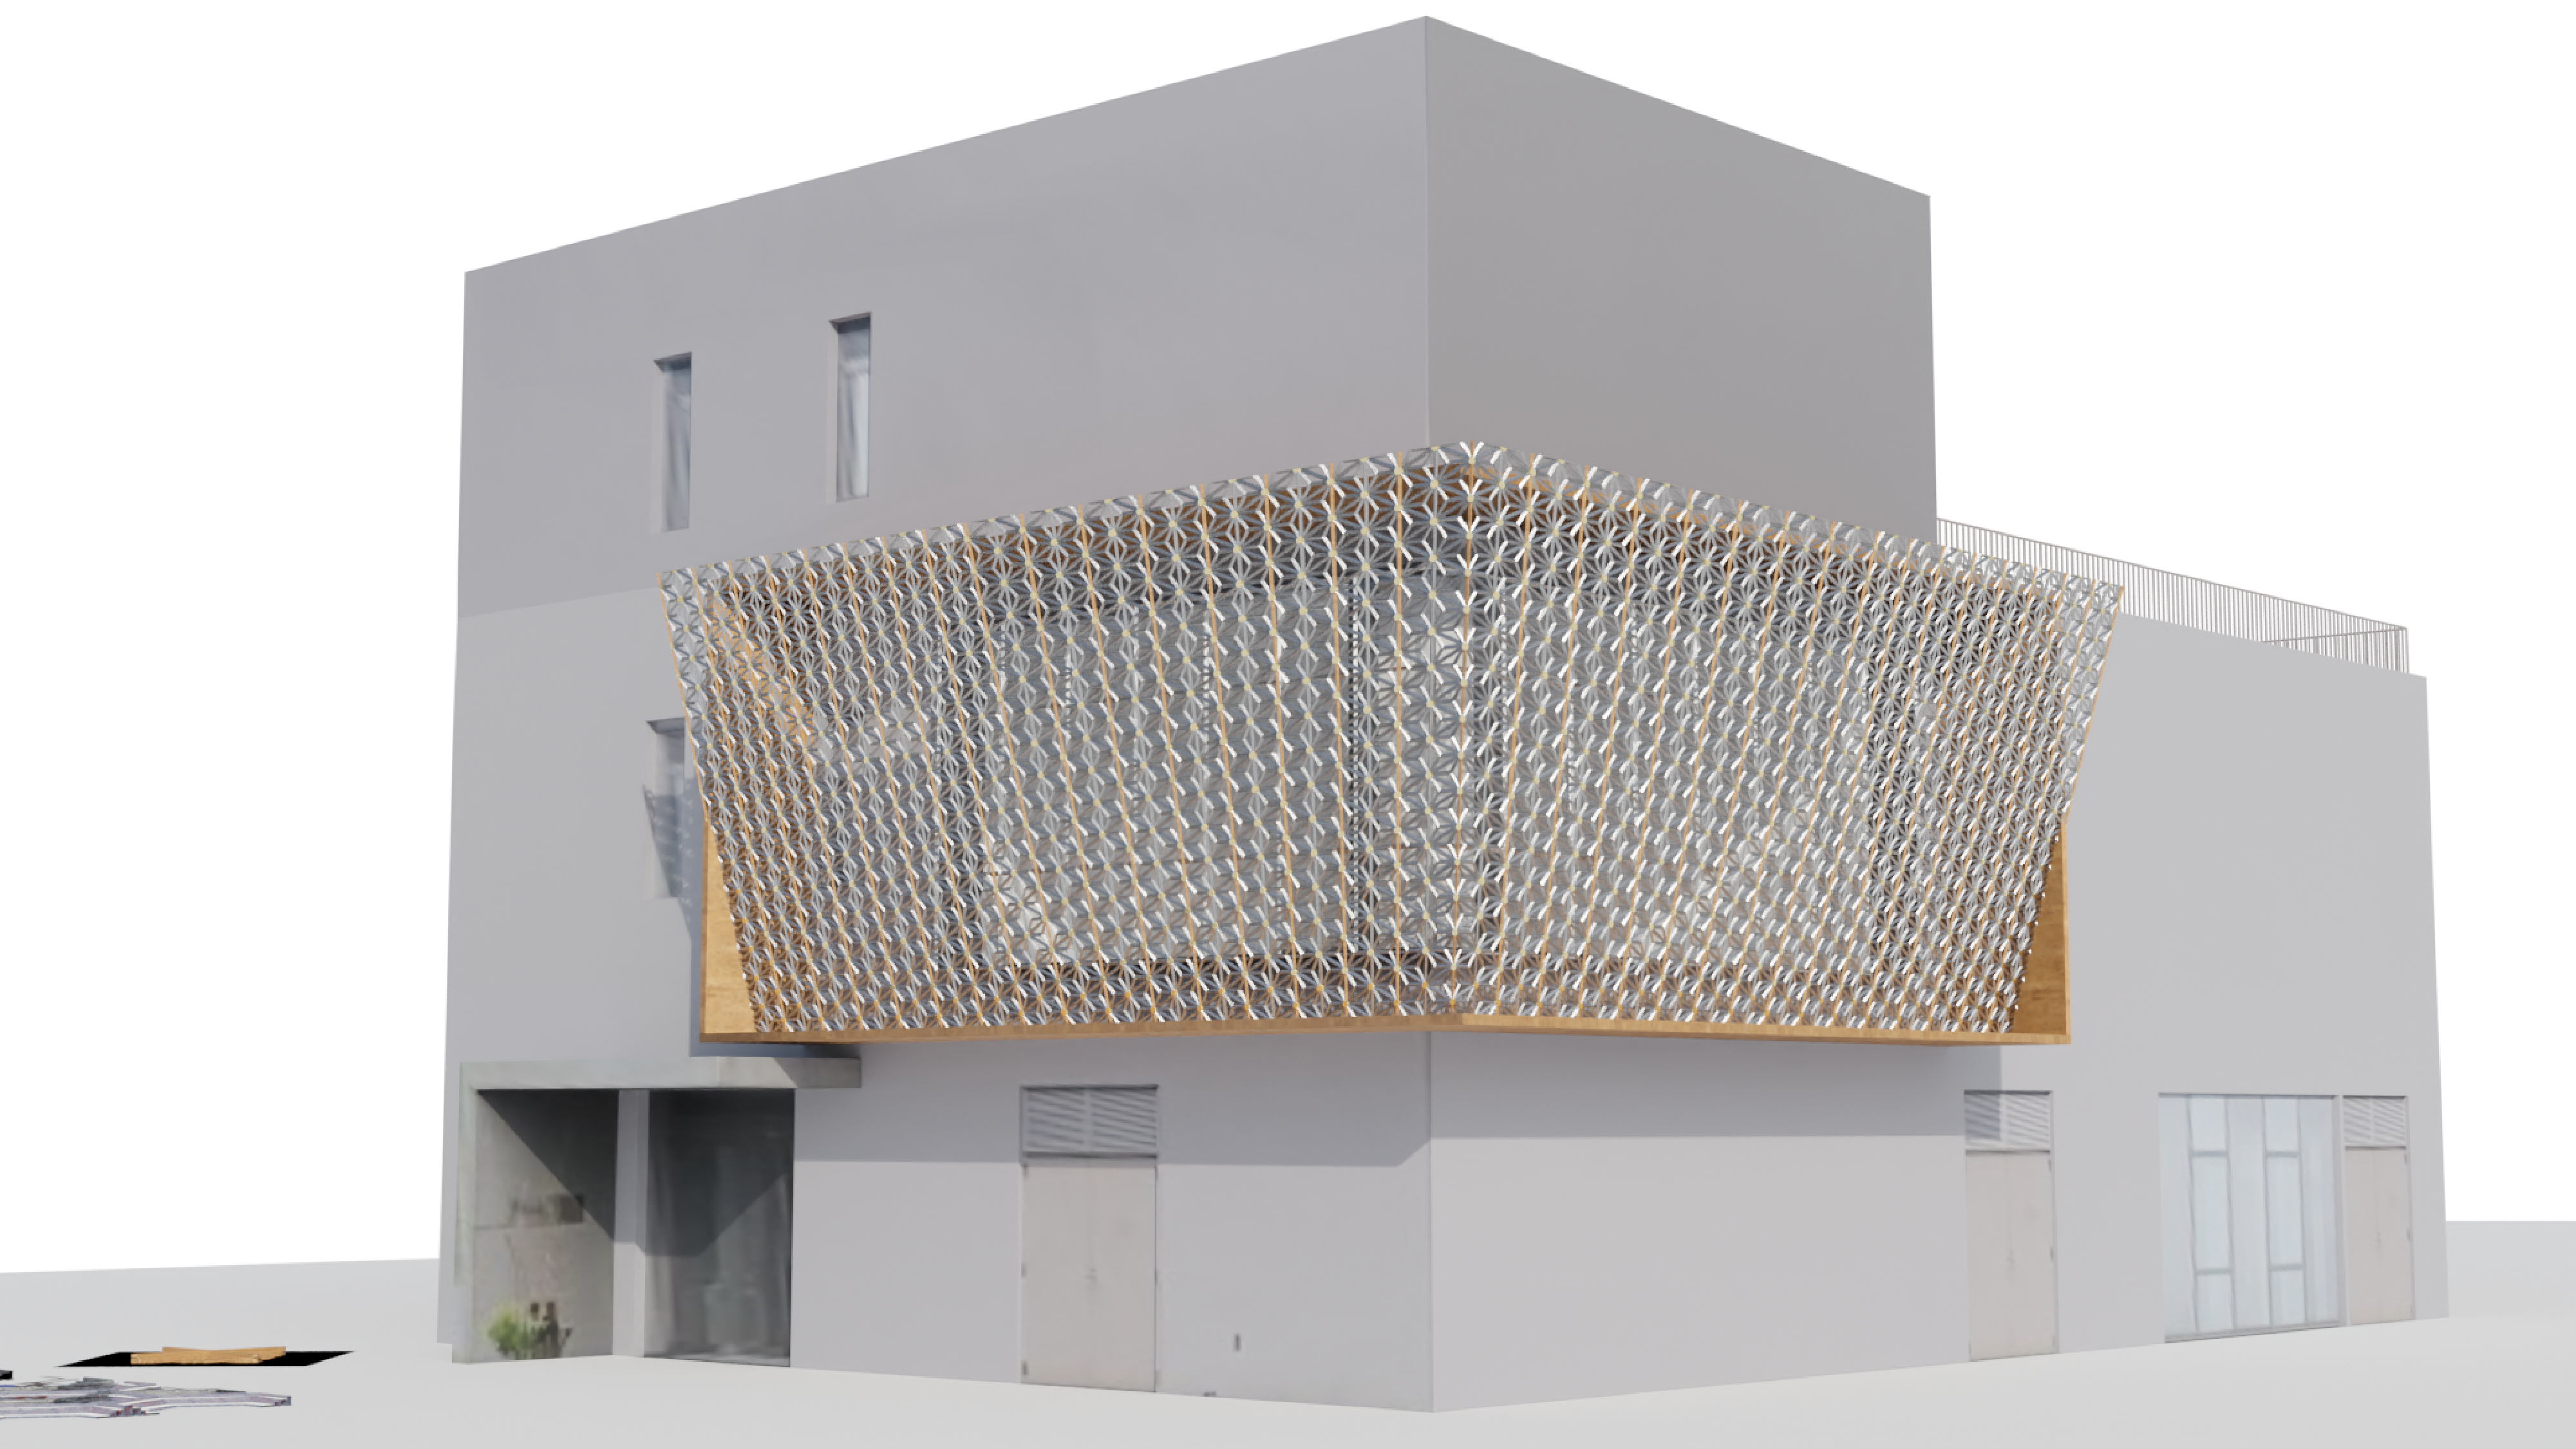
\includegraphics[width=1\linewidth]{Images/Pattern 3/0004}} \\
            \midrule
            \textit{Level 5} &  &  &
            \\
            {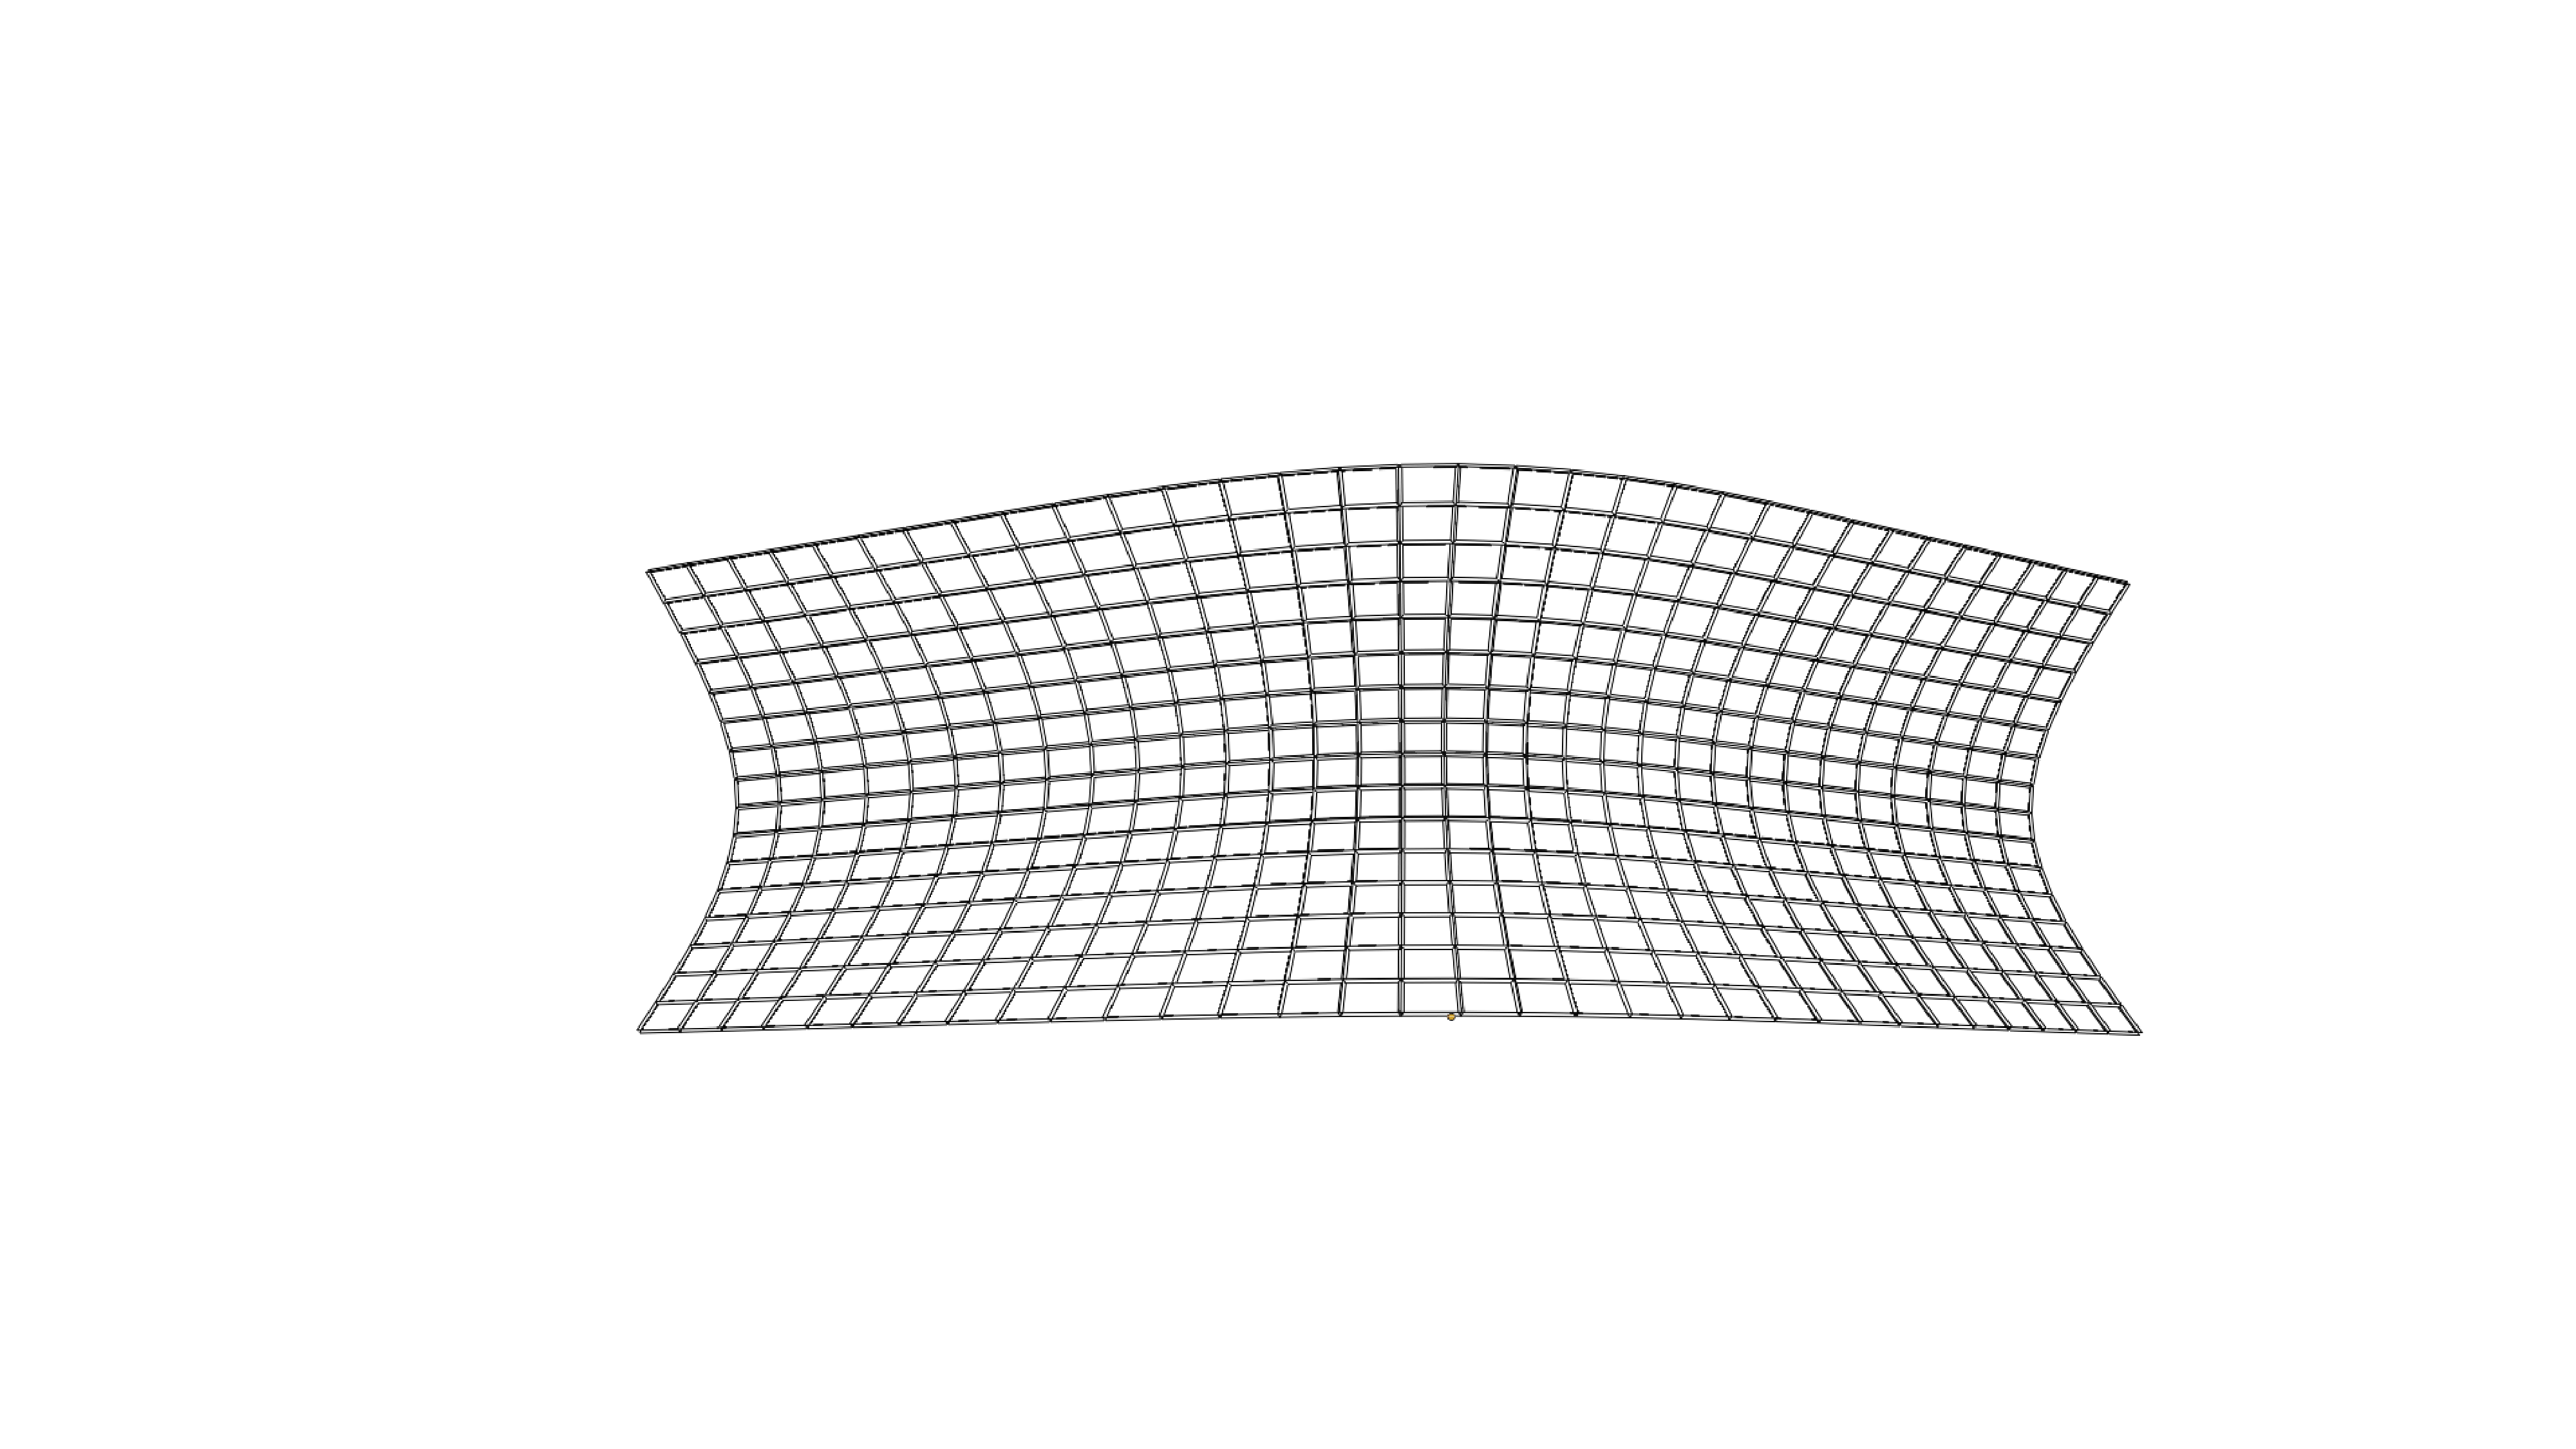
\includegraphics[width=1\linewidth]{Images/Wall 0/0005}} &
              {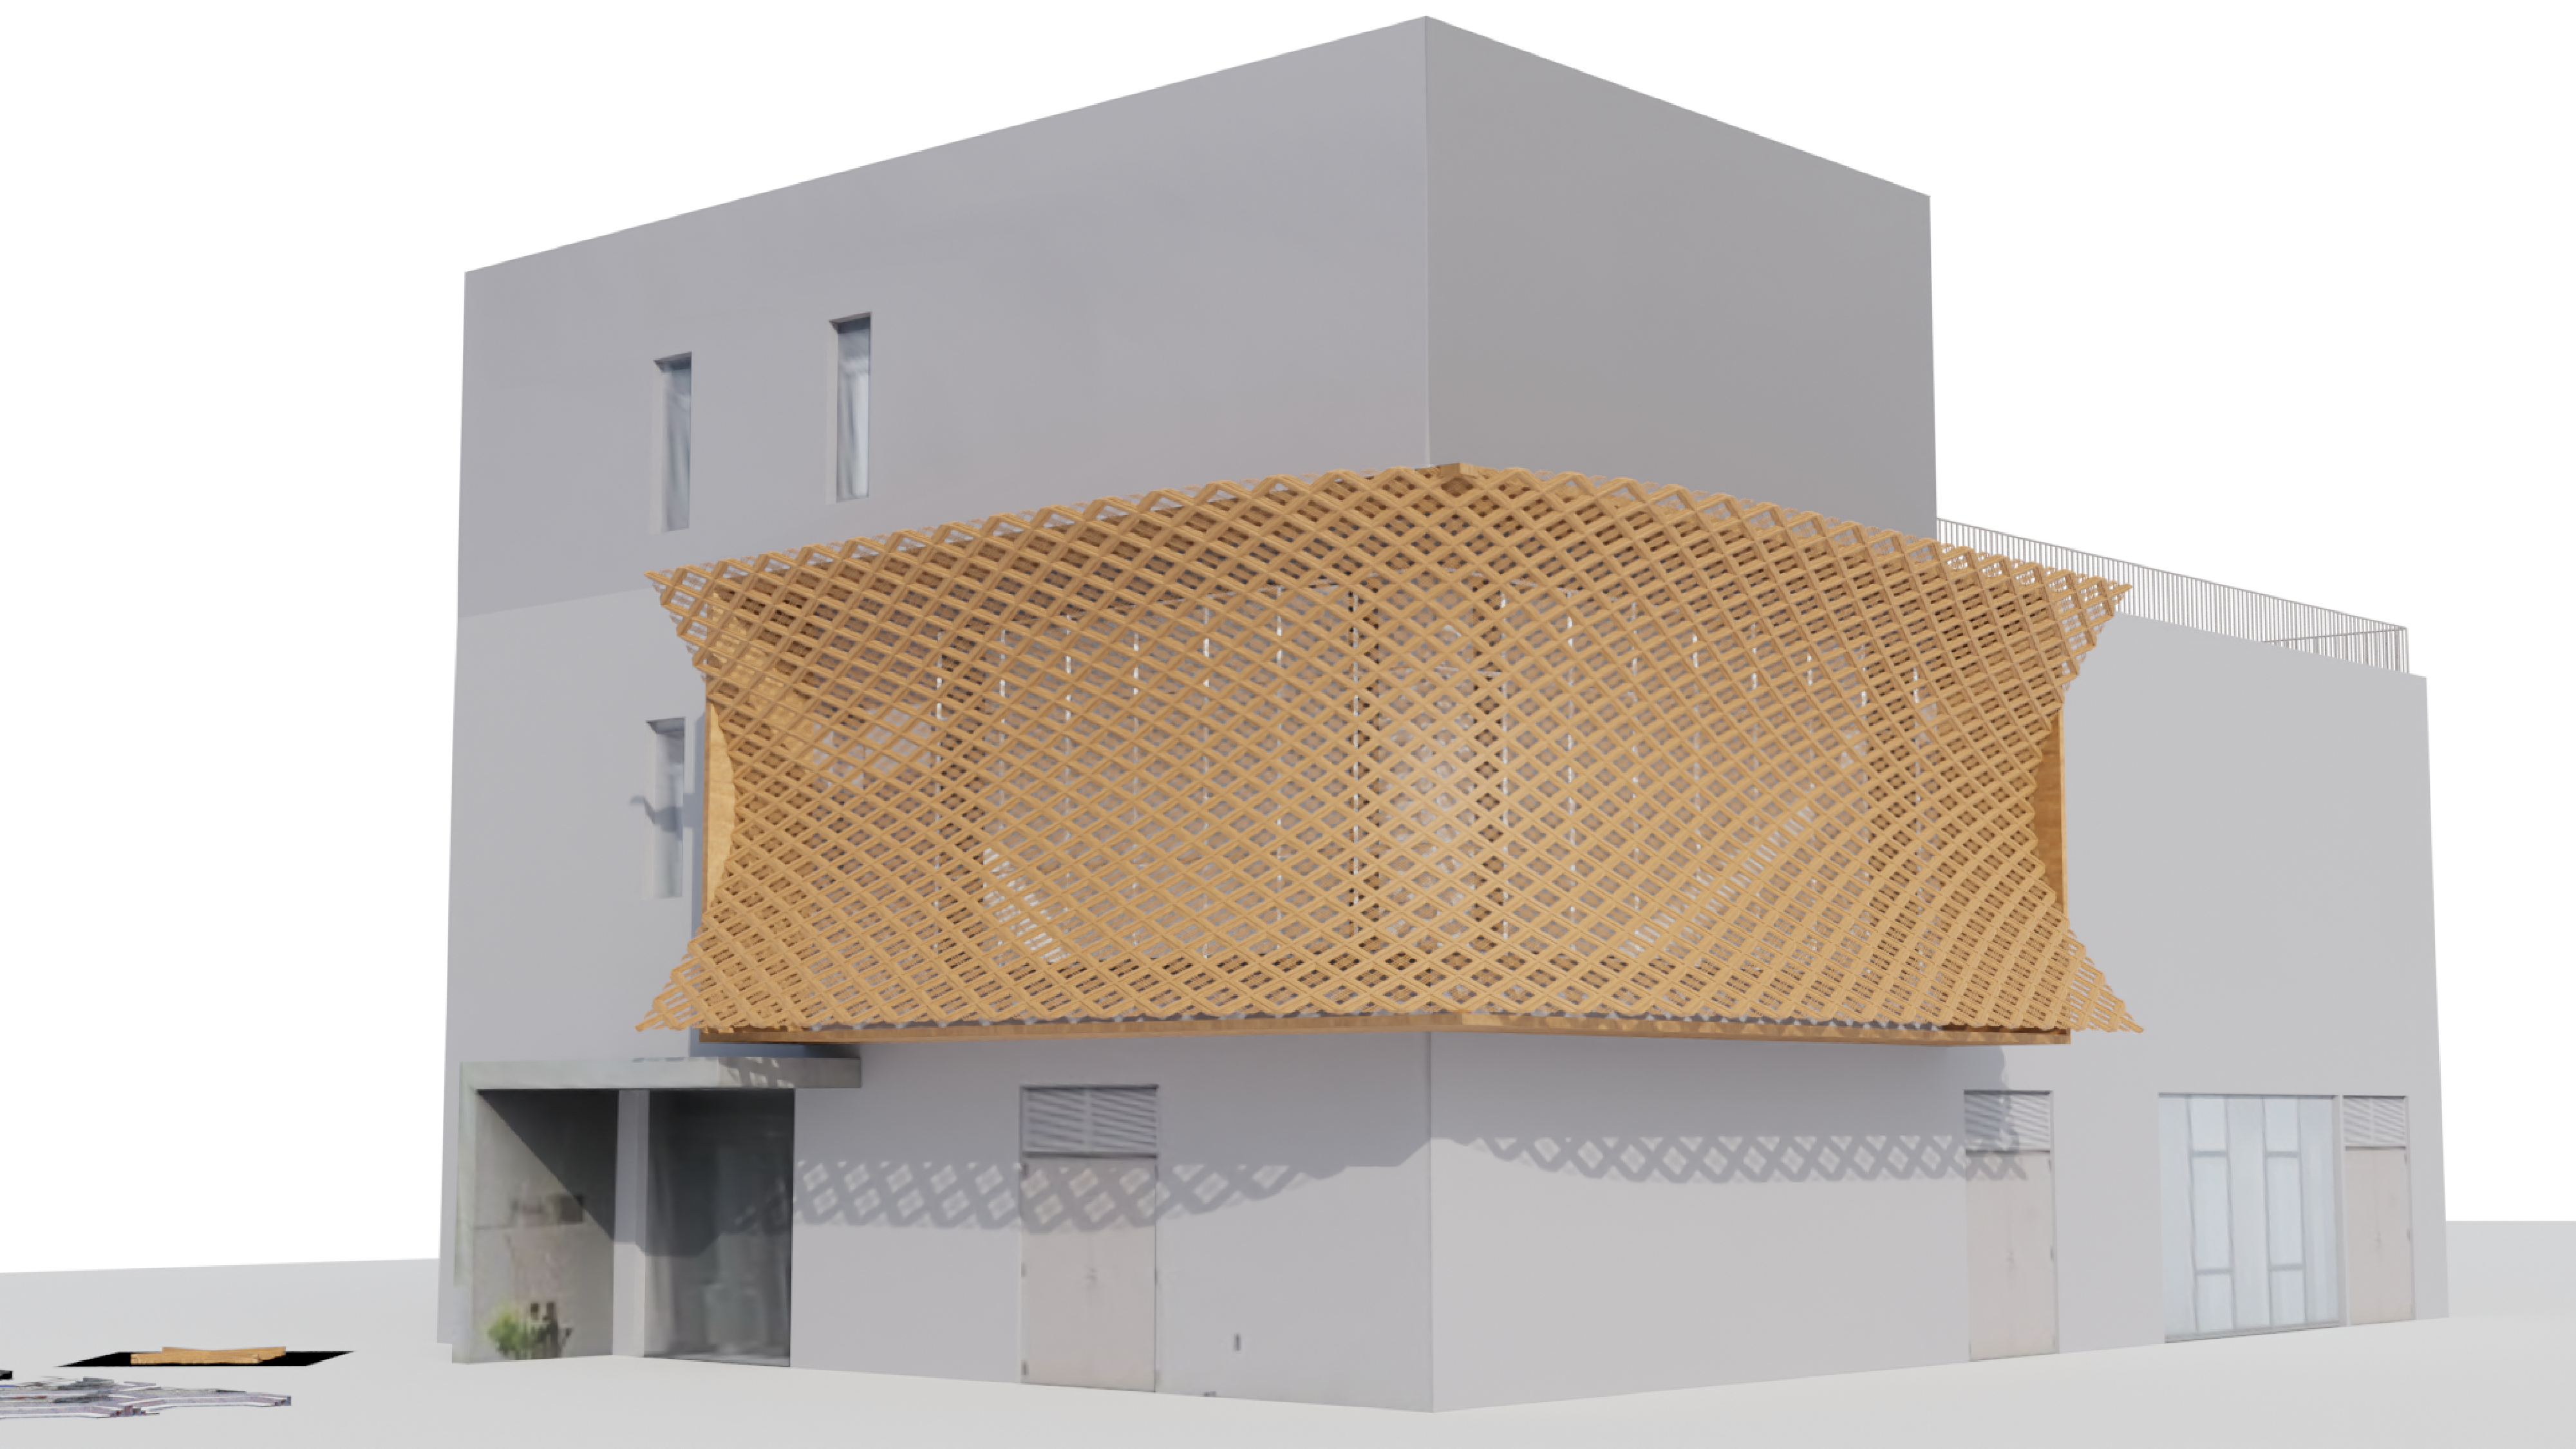
\includegraphics[width=1\linewidth]{Images/Pattern 1/0005}} &
              {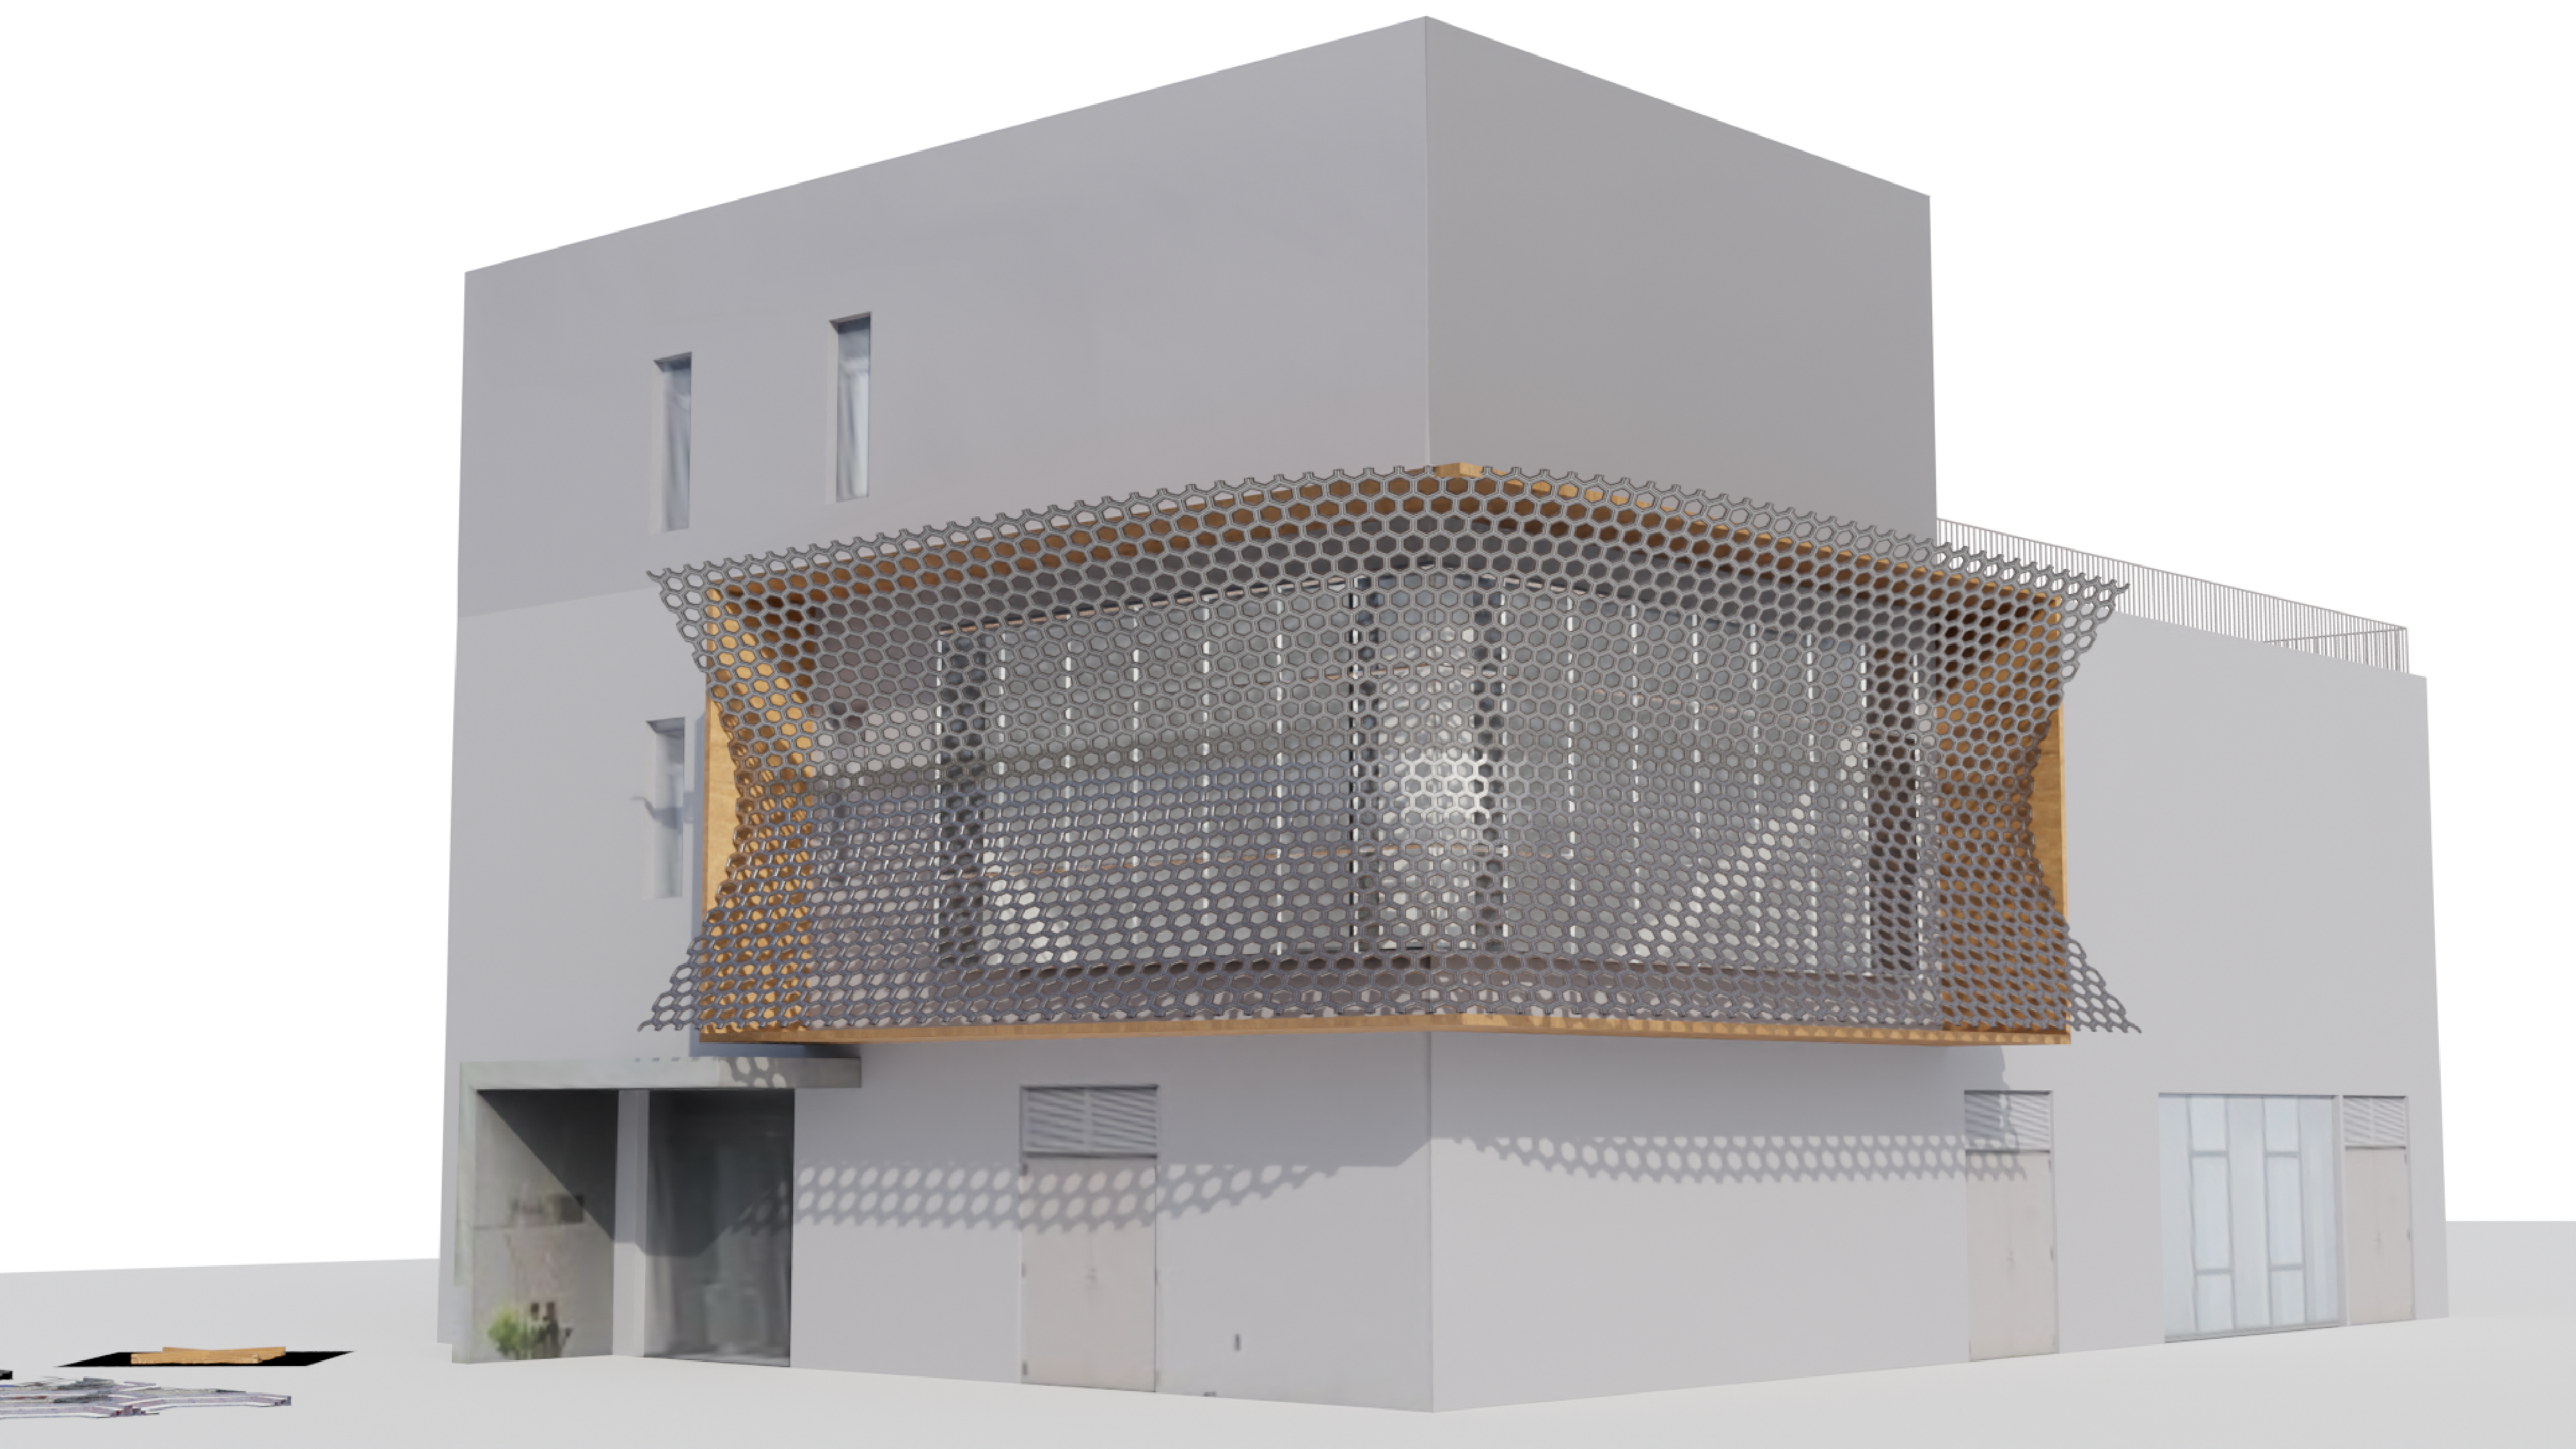
\includegraphics[width=1\linewidth]{Images/Pattern 2/0005}} &
              {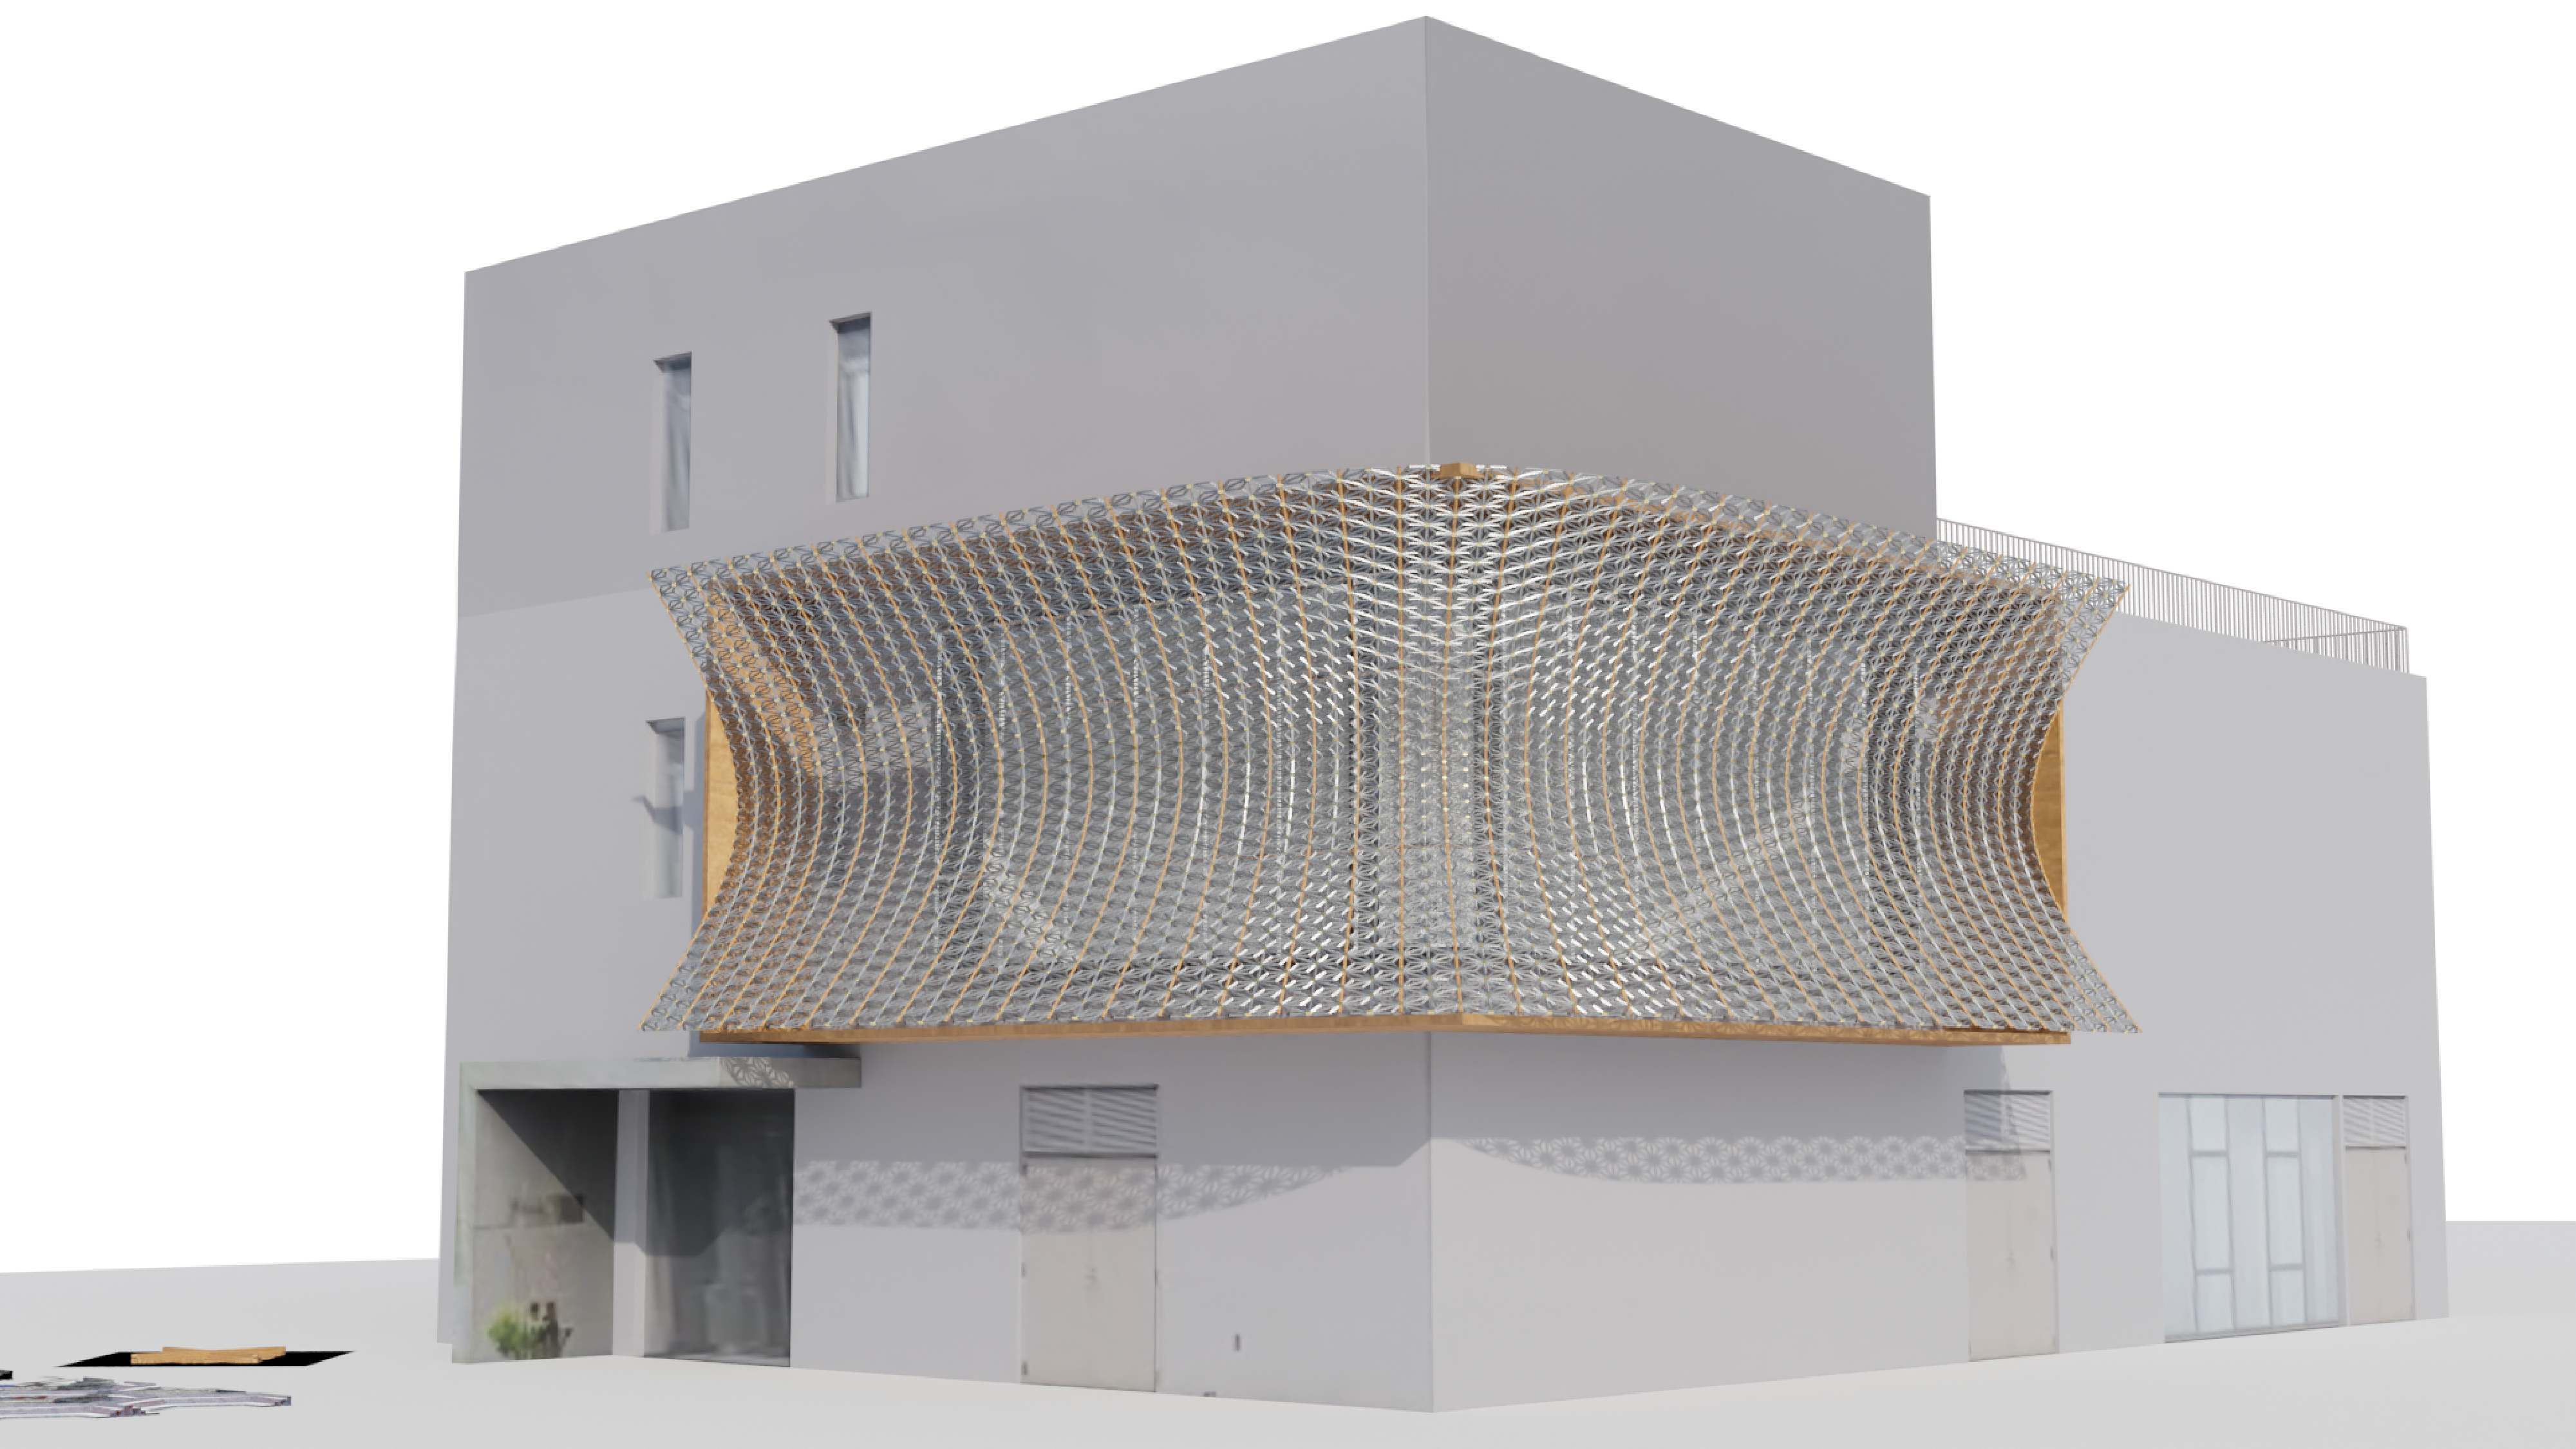
\includegraphics[width=1\linewidth]{Images/Pattern 3/0005}} \\
            \bottomrule
        \end{tabularx}
    \end{table*}

    %%Table: Pattern Variations 6 to 10. Part2
    \begin{table*}[htb]
        \centering
        \small
        \caption{Patterns variations for the last five levels of complexity}
        \label{tab:PatternsVariationsPart2}
        \begin{tabularx}
        {\textwidth}{p{3cm} >{\centering\arraybackslash}X >{\centering\arraybackslash}X >{\centering\arraybackslash}X }
            \toprule
            \textit{Description} &
              \textit{Pattern 1} &
              \textit{Pattern 2} &
              \textit{Pattern 3} \\
            \midrule
            \text{Pattern Name} & Hishi Pattern & Tortoise shells & Asanoha Pattern\\

            \midrule
            \textit{Base Module} &  &  &
            \\
            {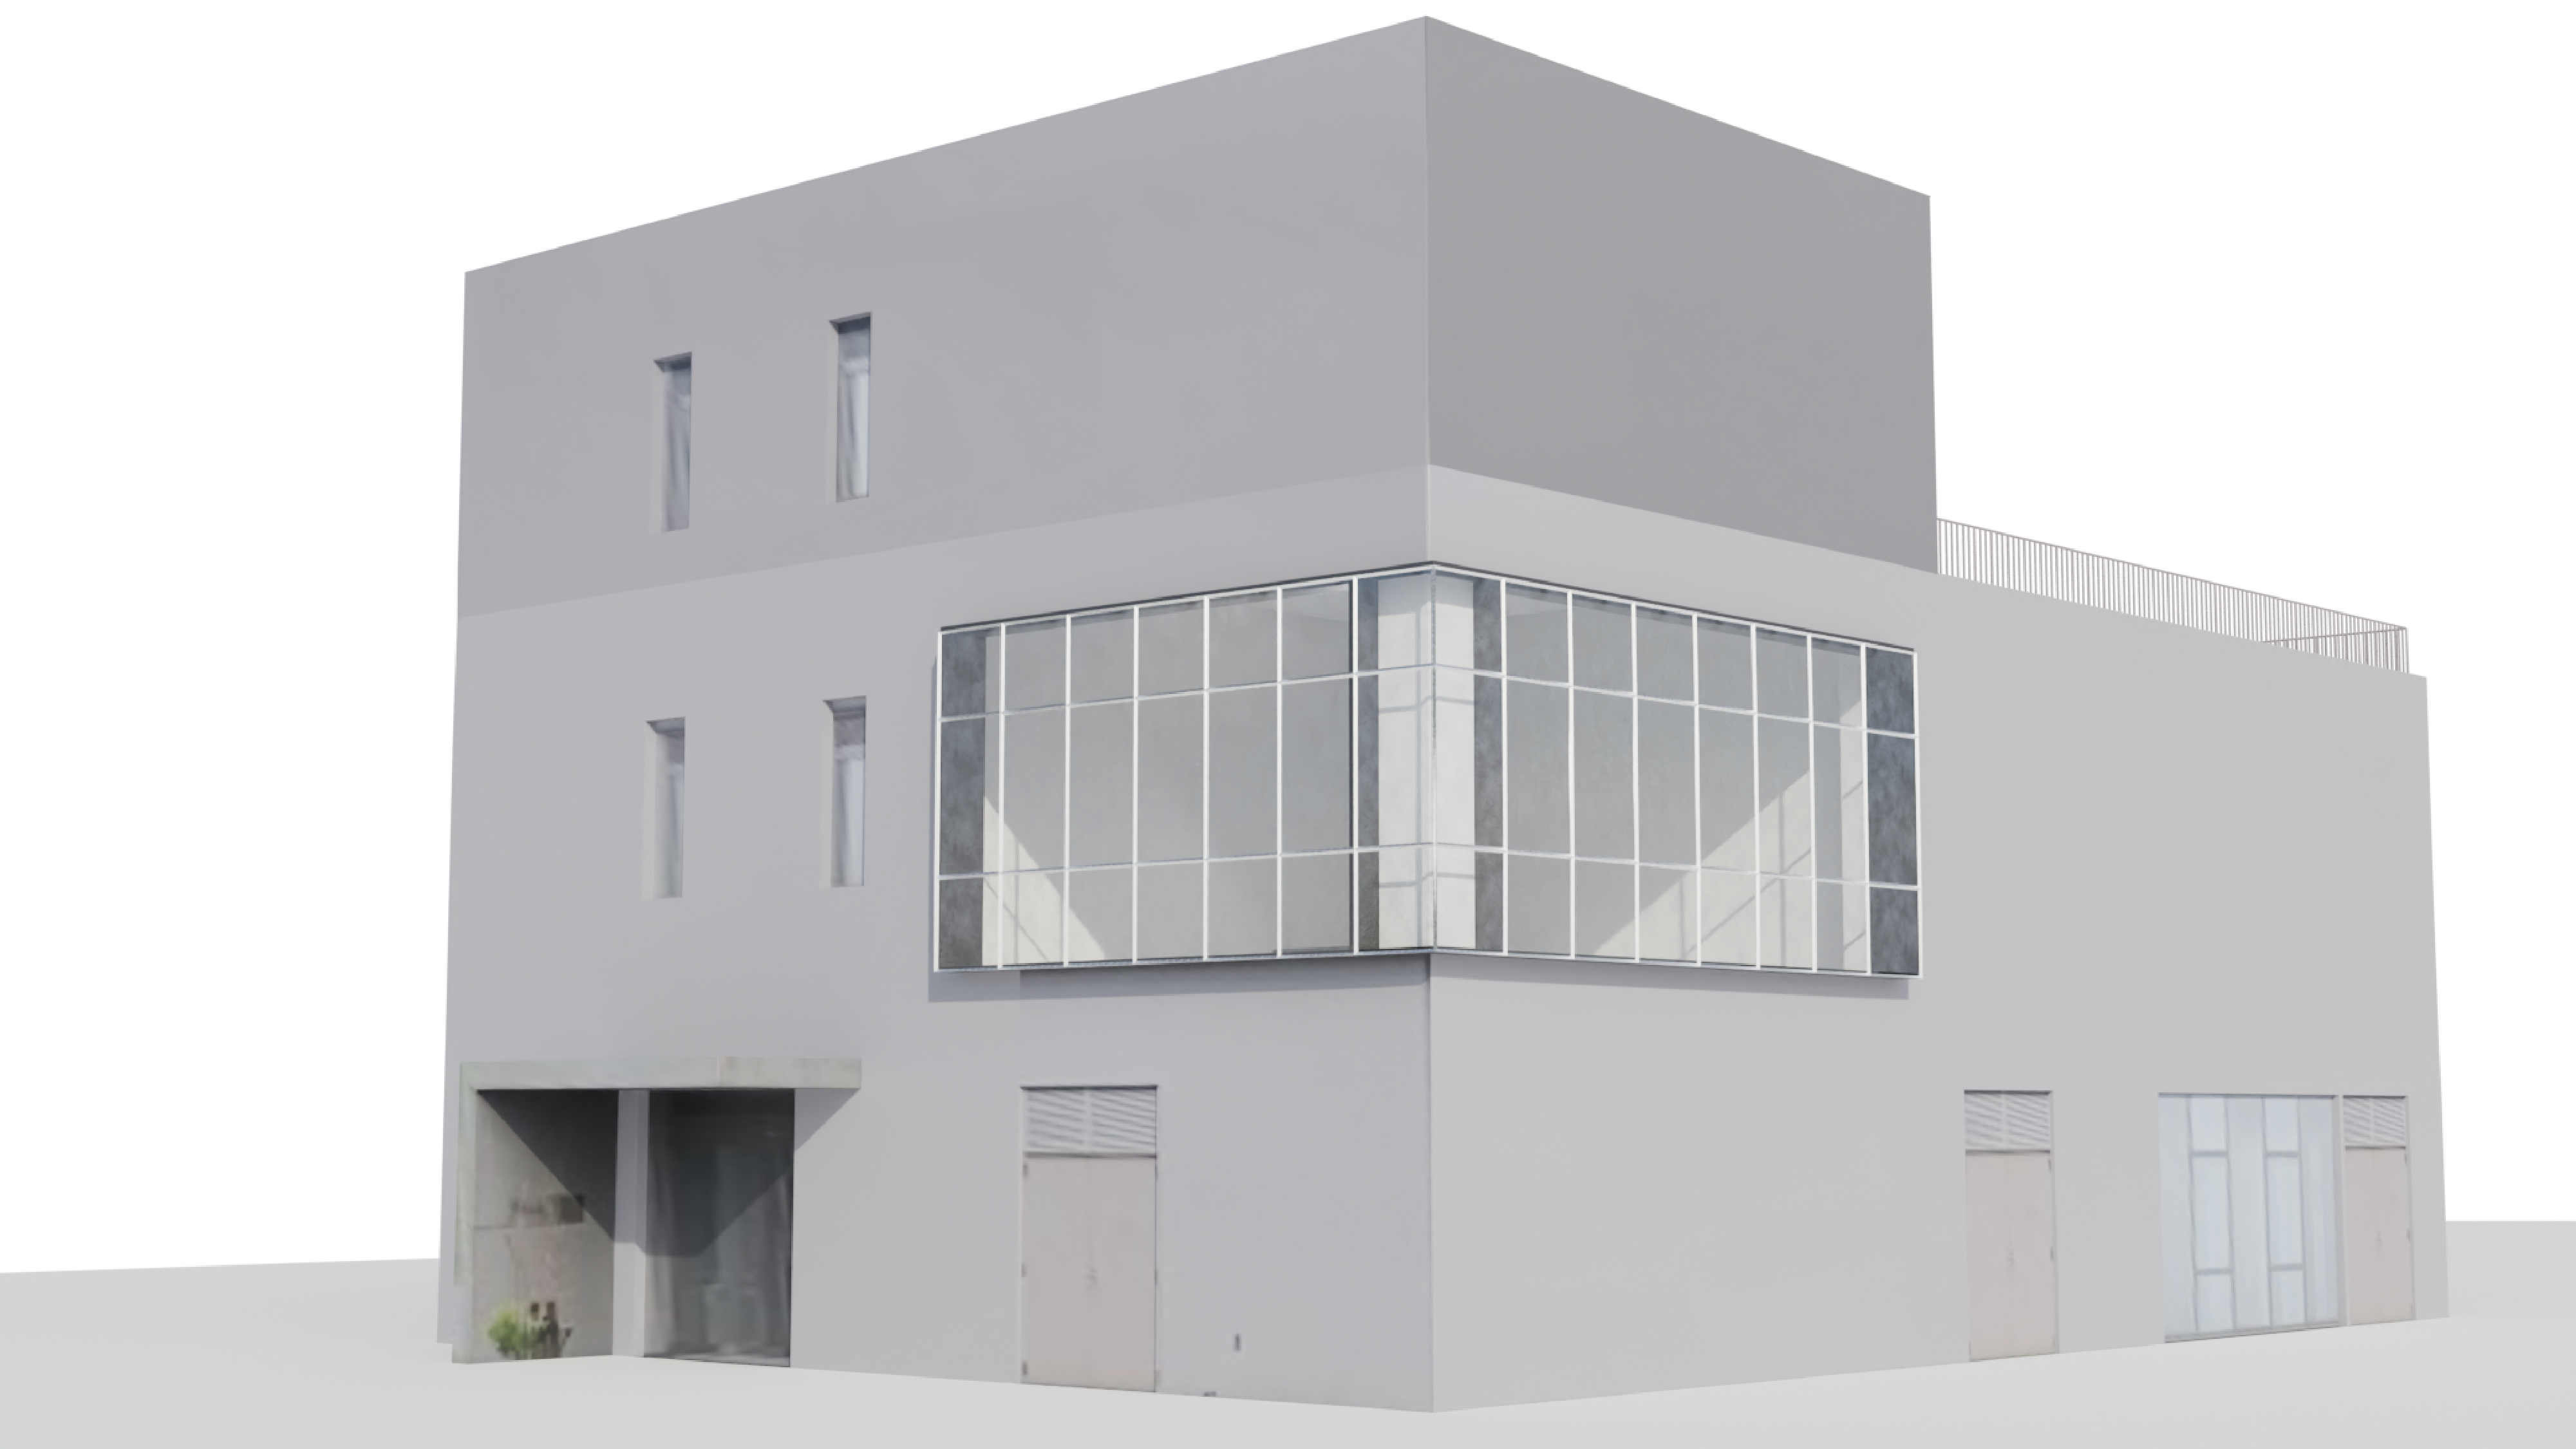
\includegraphics[width=1\linewidth]{Images/Base Module/Building}} &
              {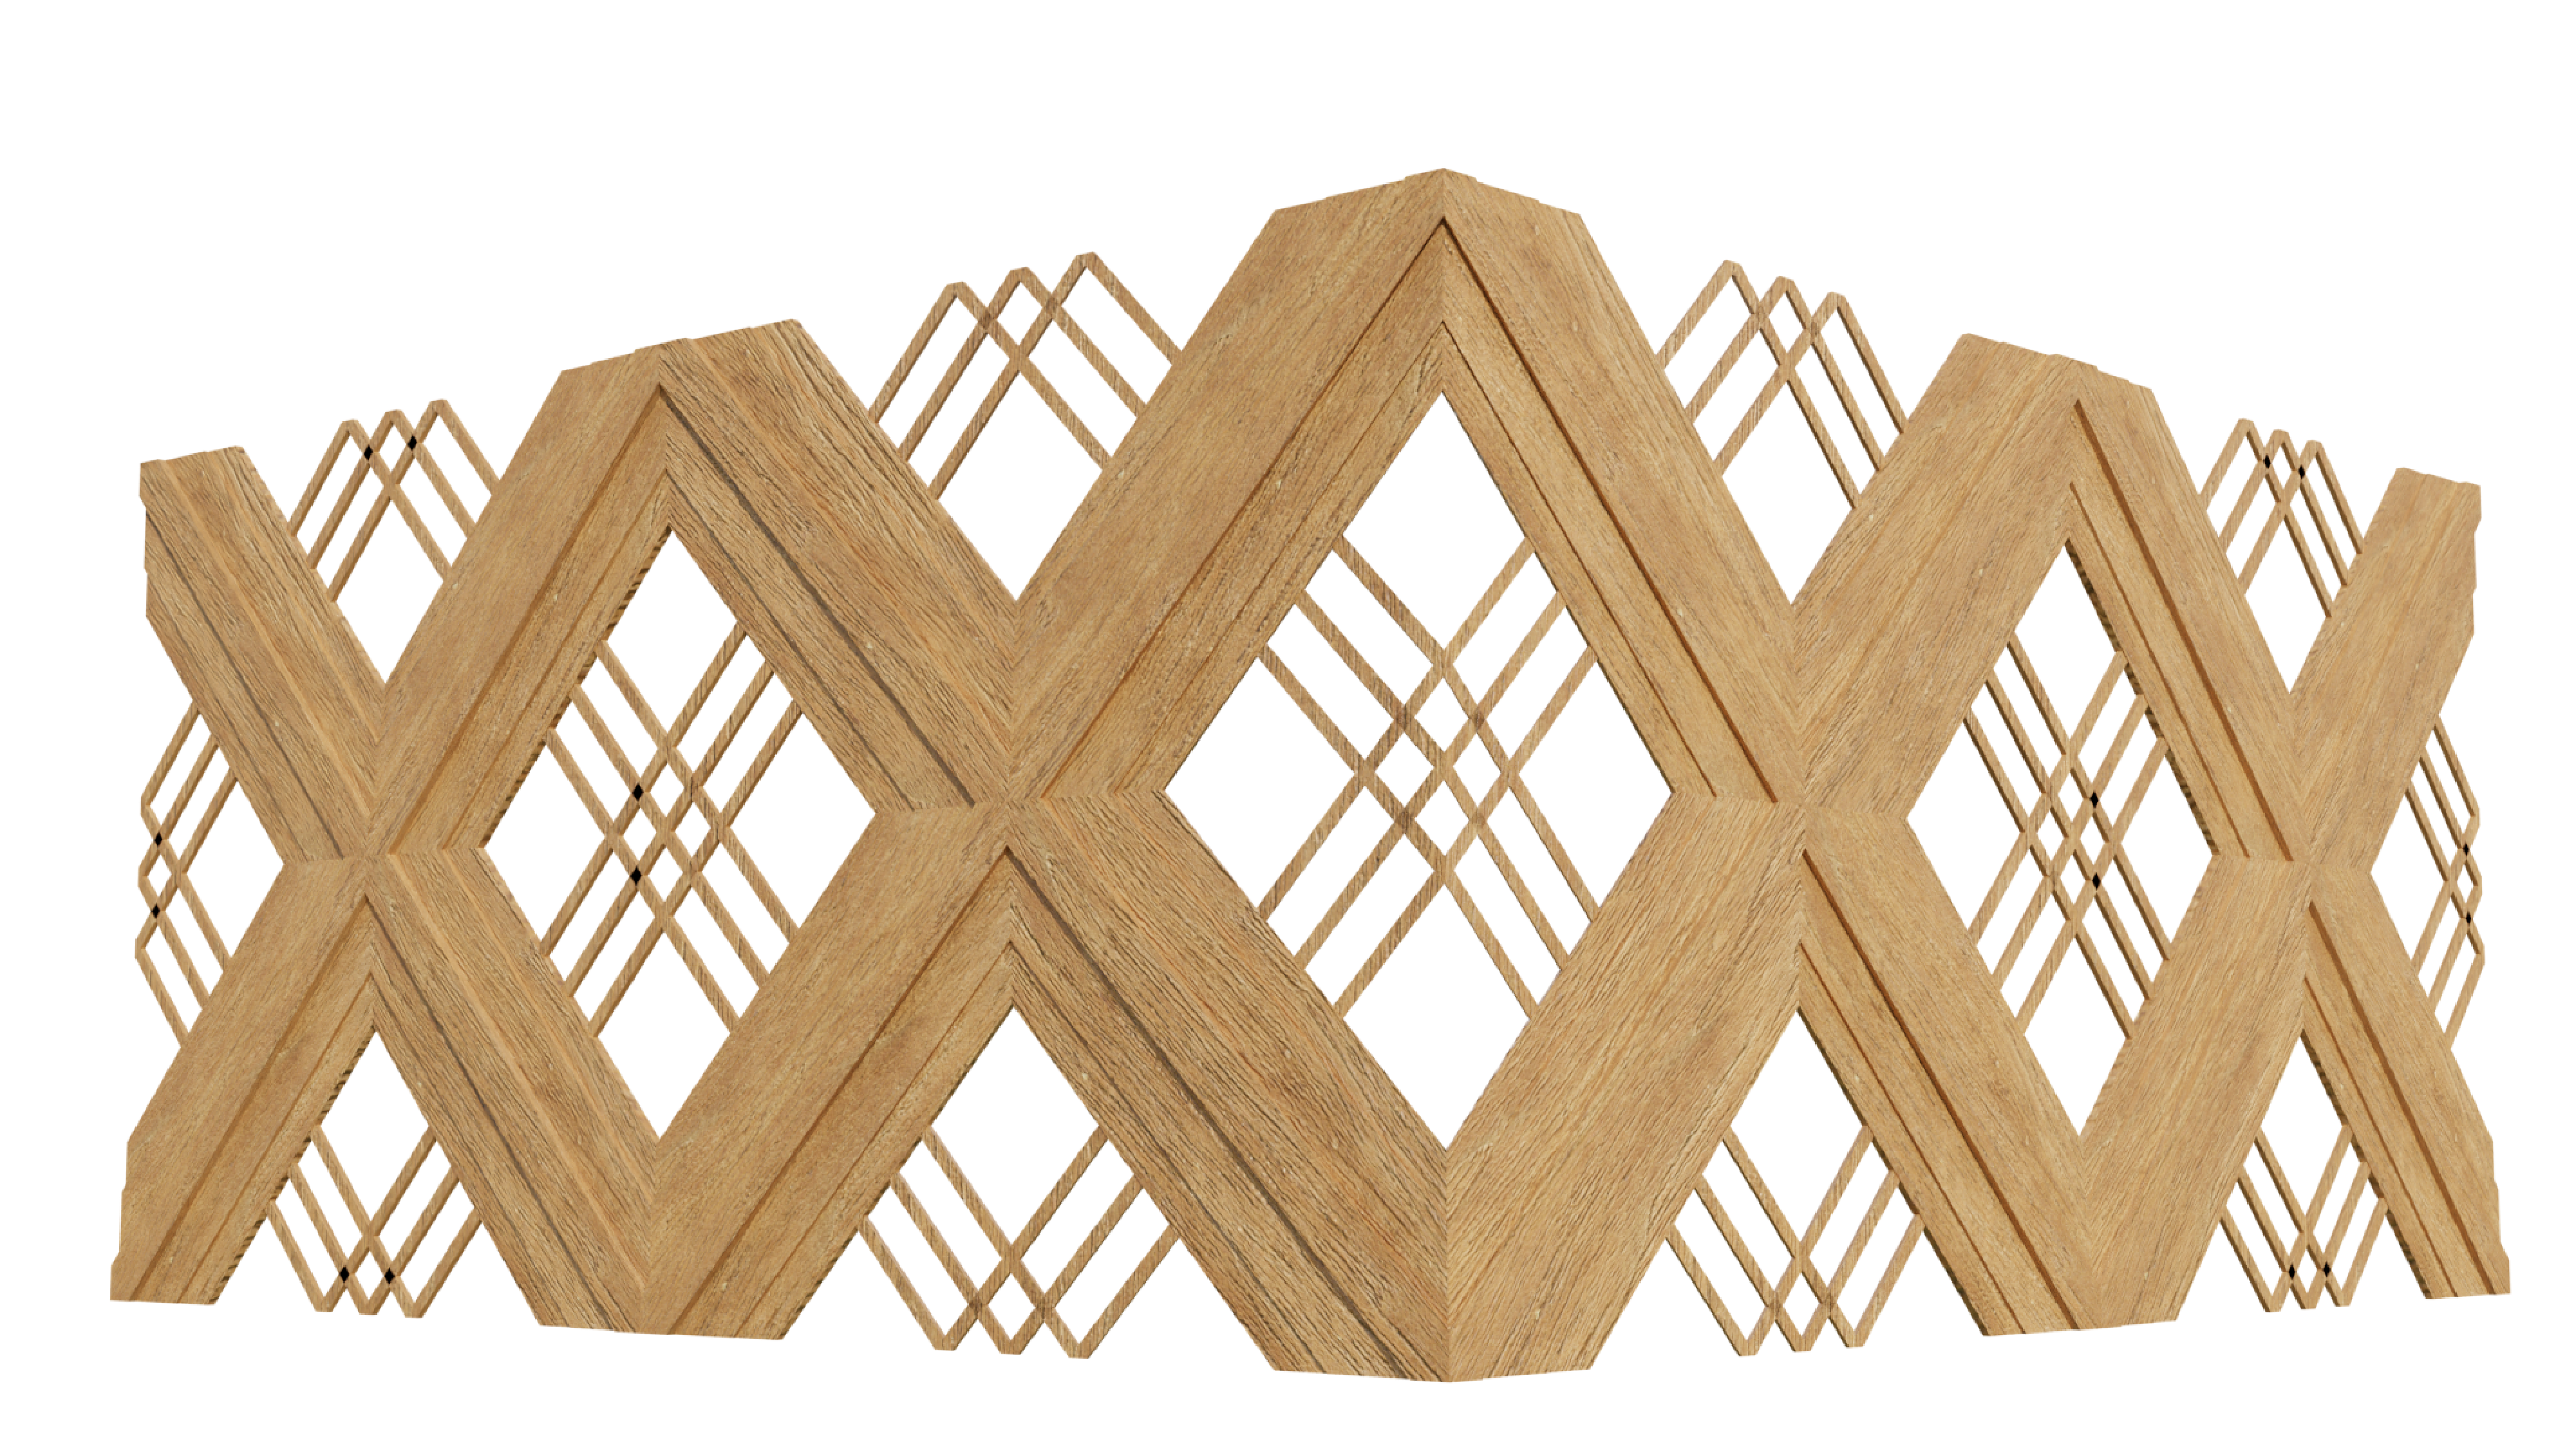
\includegraphics[width=1\linewidth]{Images/Base Module/Pattern1}} &
              {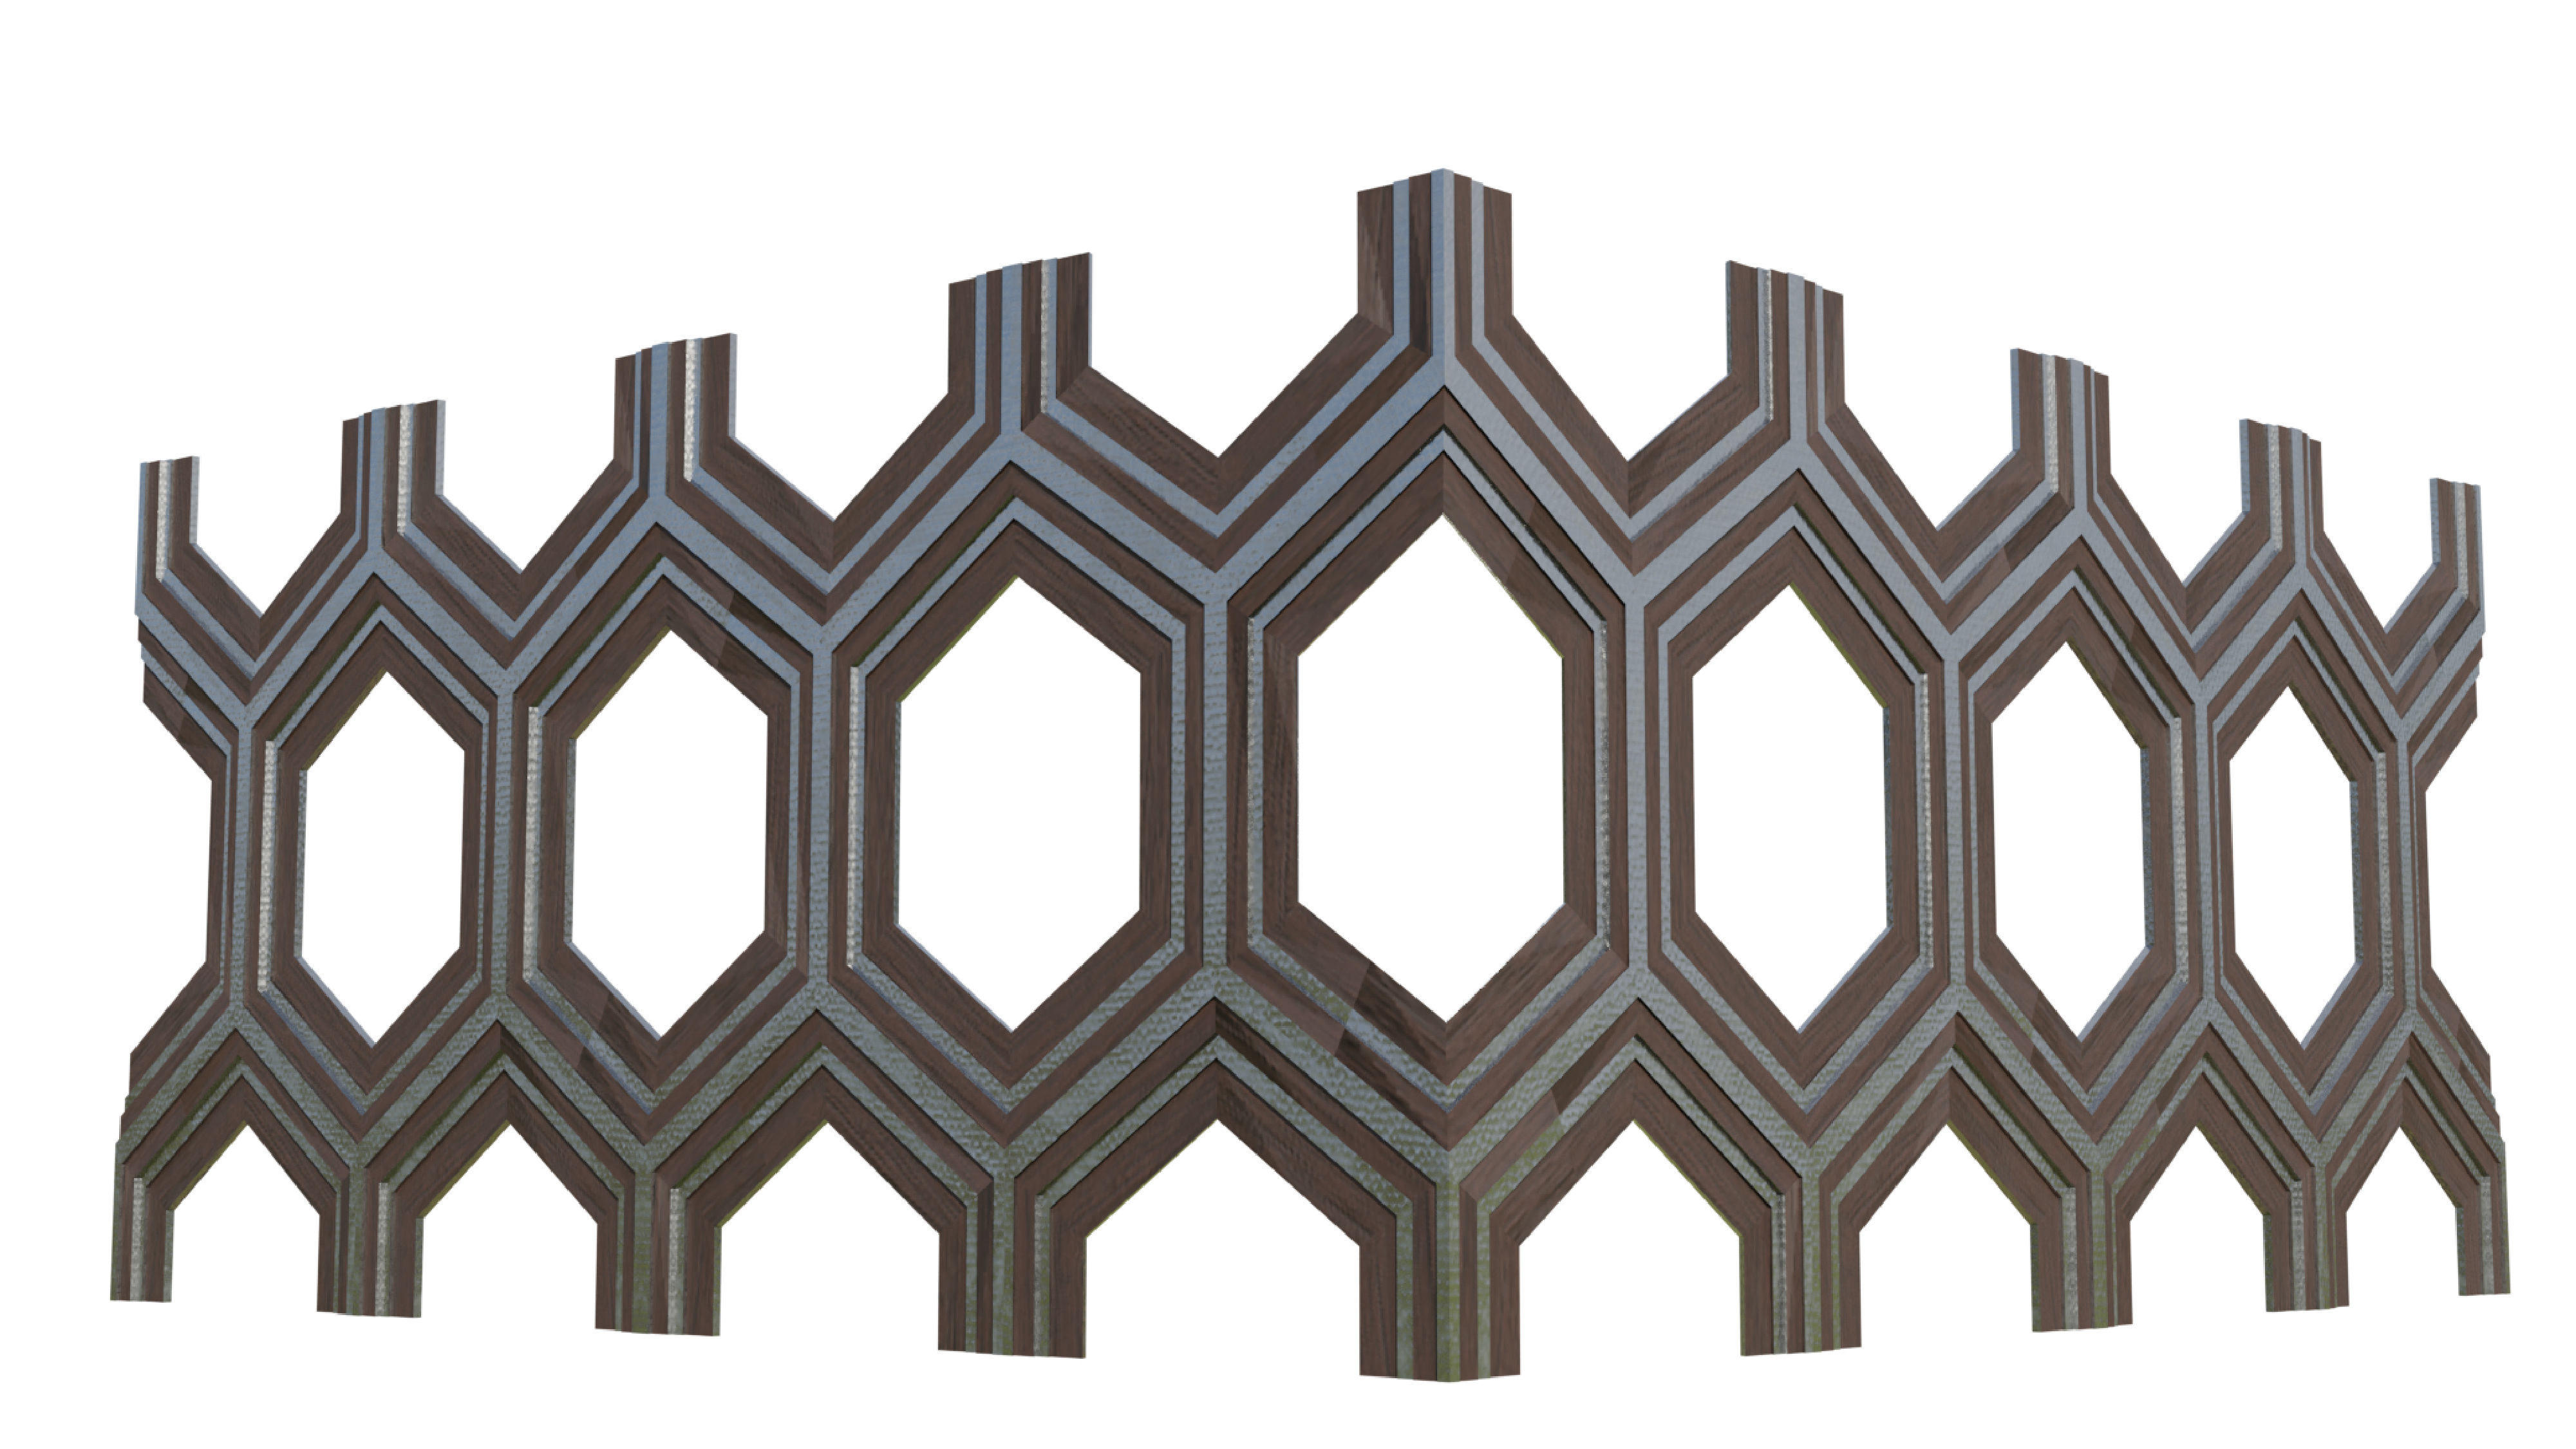
\includegraphics[width=1\linewidth]{Images/Base Module/Pattern2}} &
              {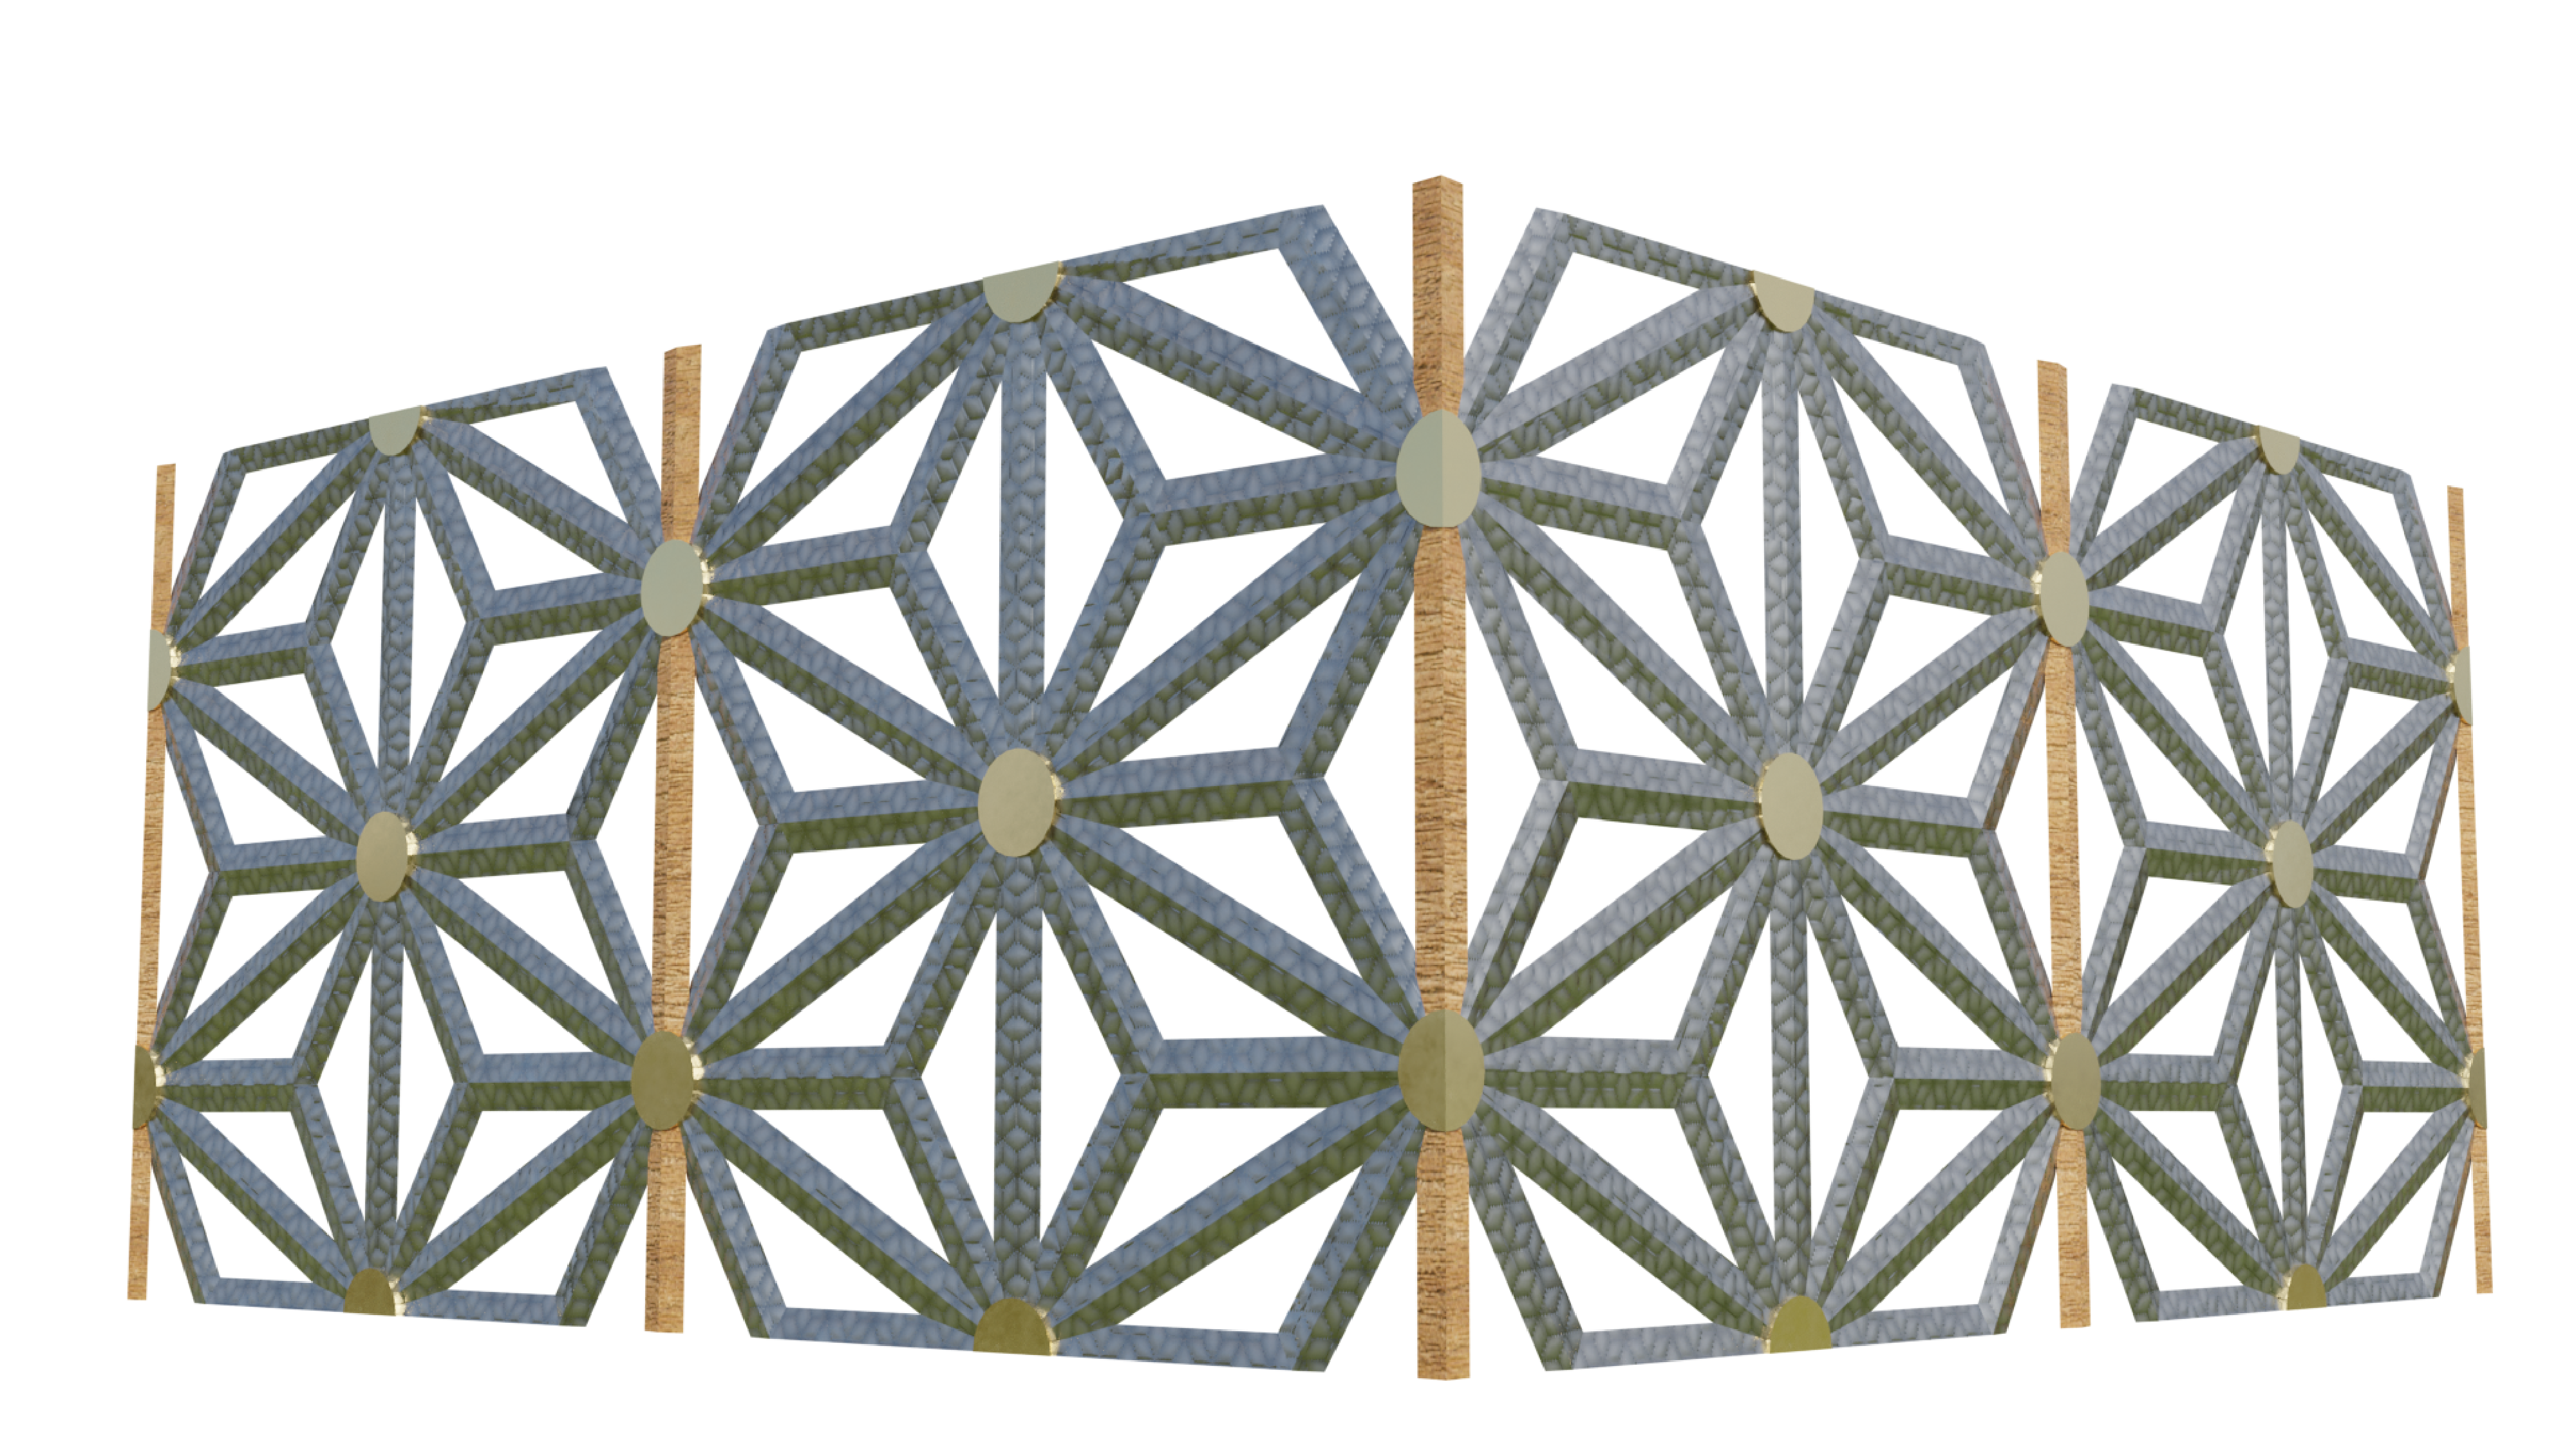
\includegraphics[width=1\linewidth]{Images/Base Module/Pattern3}} \\
            \midrule

            \textit{Mesh complexity Level} &
              \textit{Pattern 1} &
              \textit{Pattern 2} &
              \textit{Pattern 3}\\

            \midrule
            \textit{Level 6} &  &  &
            \\
            {\includegraphics[width=1\linewidth]{Images/Wall 0/0006}} &
                {\includegraphics[width=1\linewidth]{Images/Pattern 1/0006}} &
              {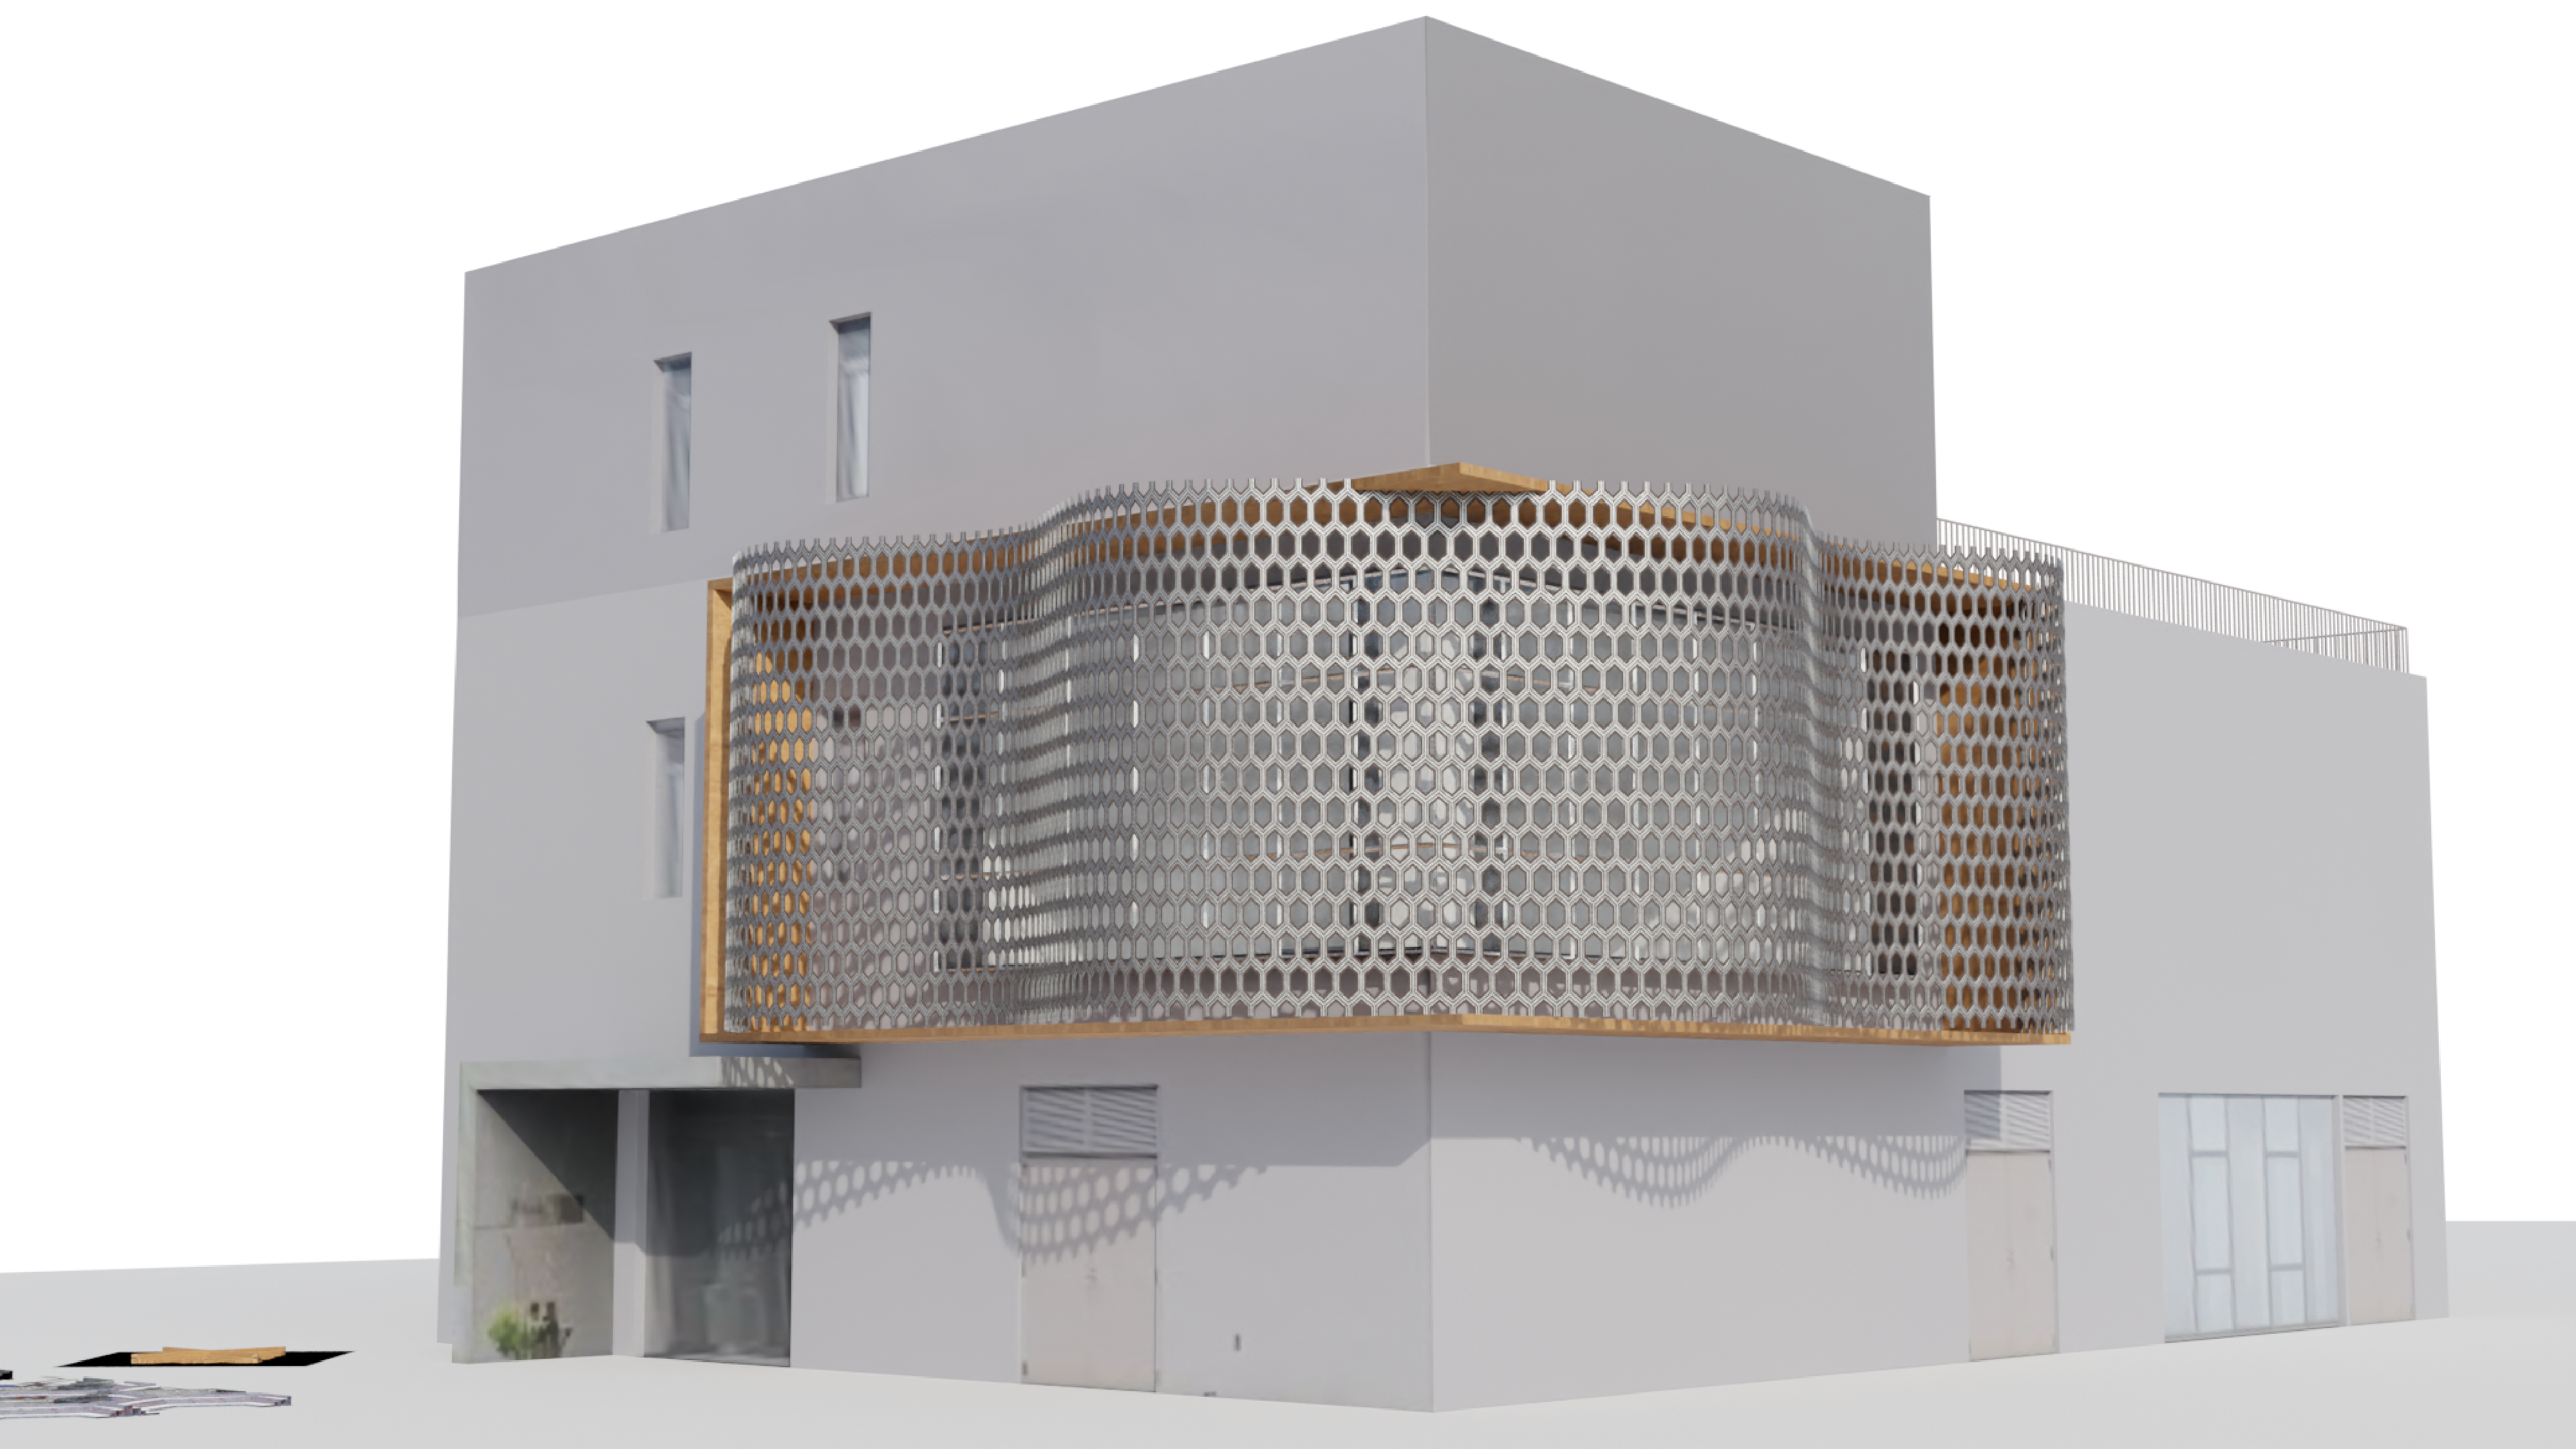
\includegraphics[width=1\linewidth]{Images/Pattern 2/0006}} &
              {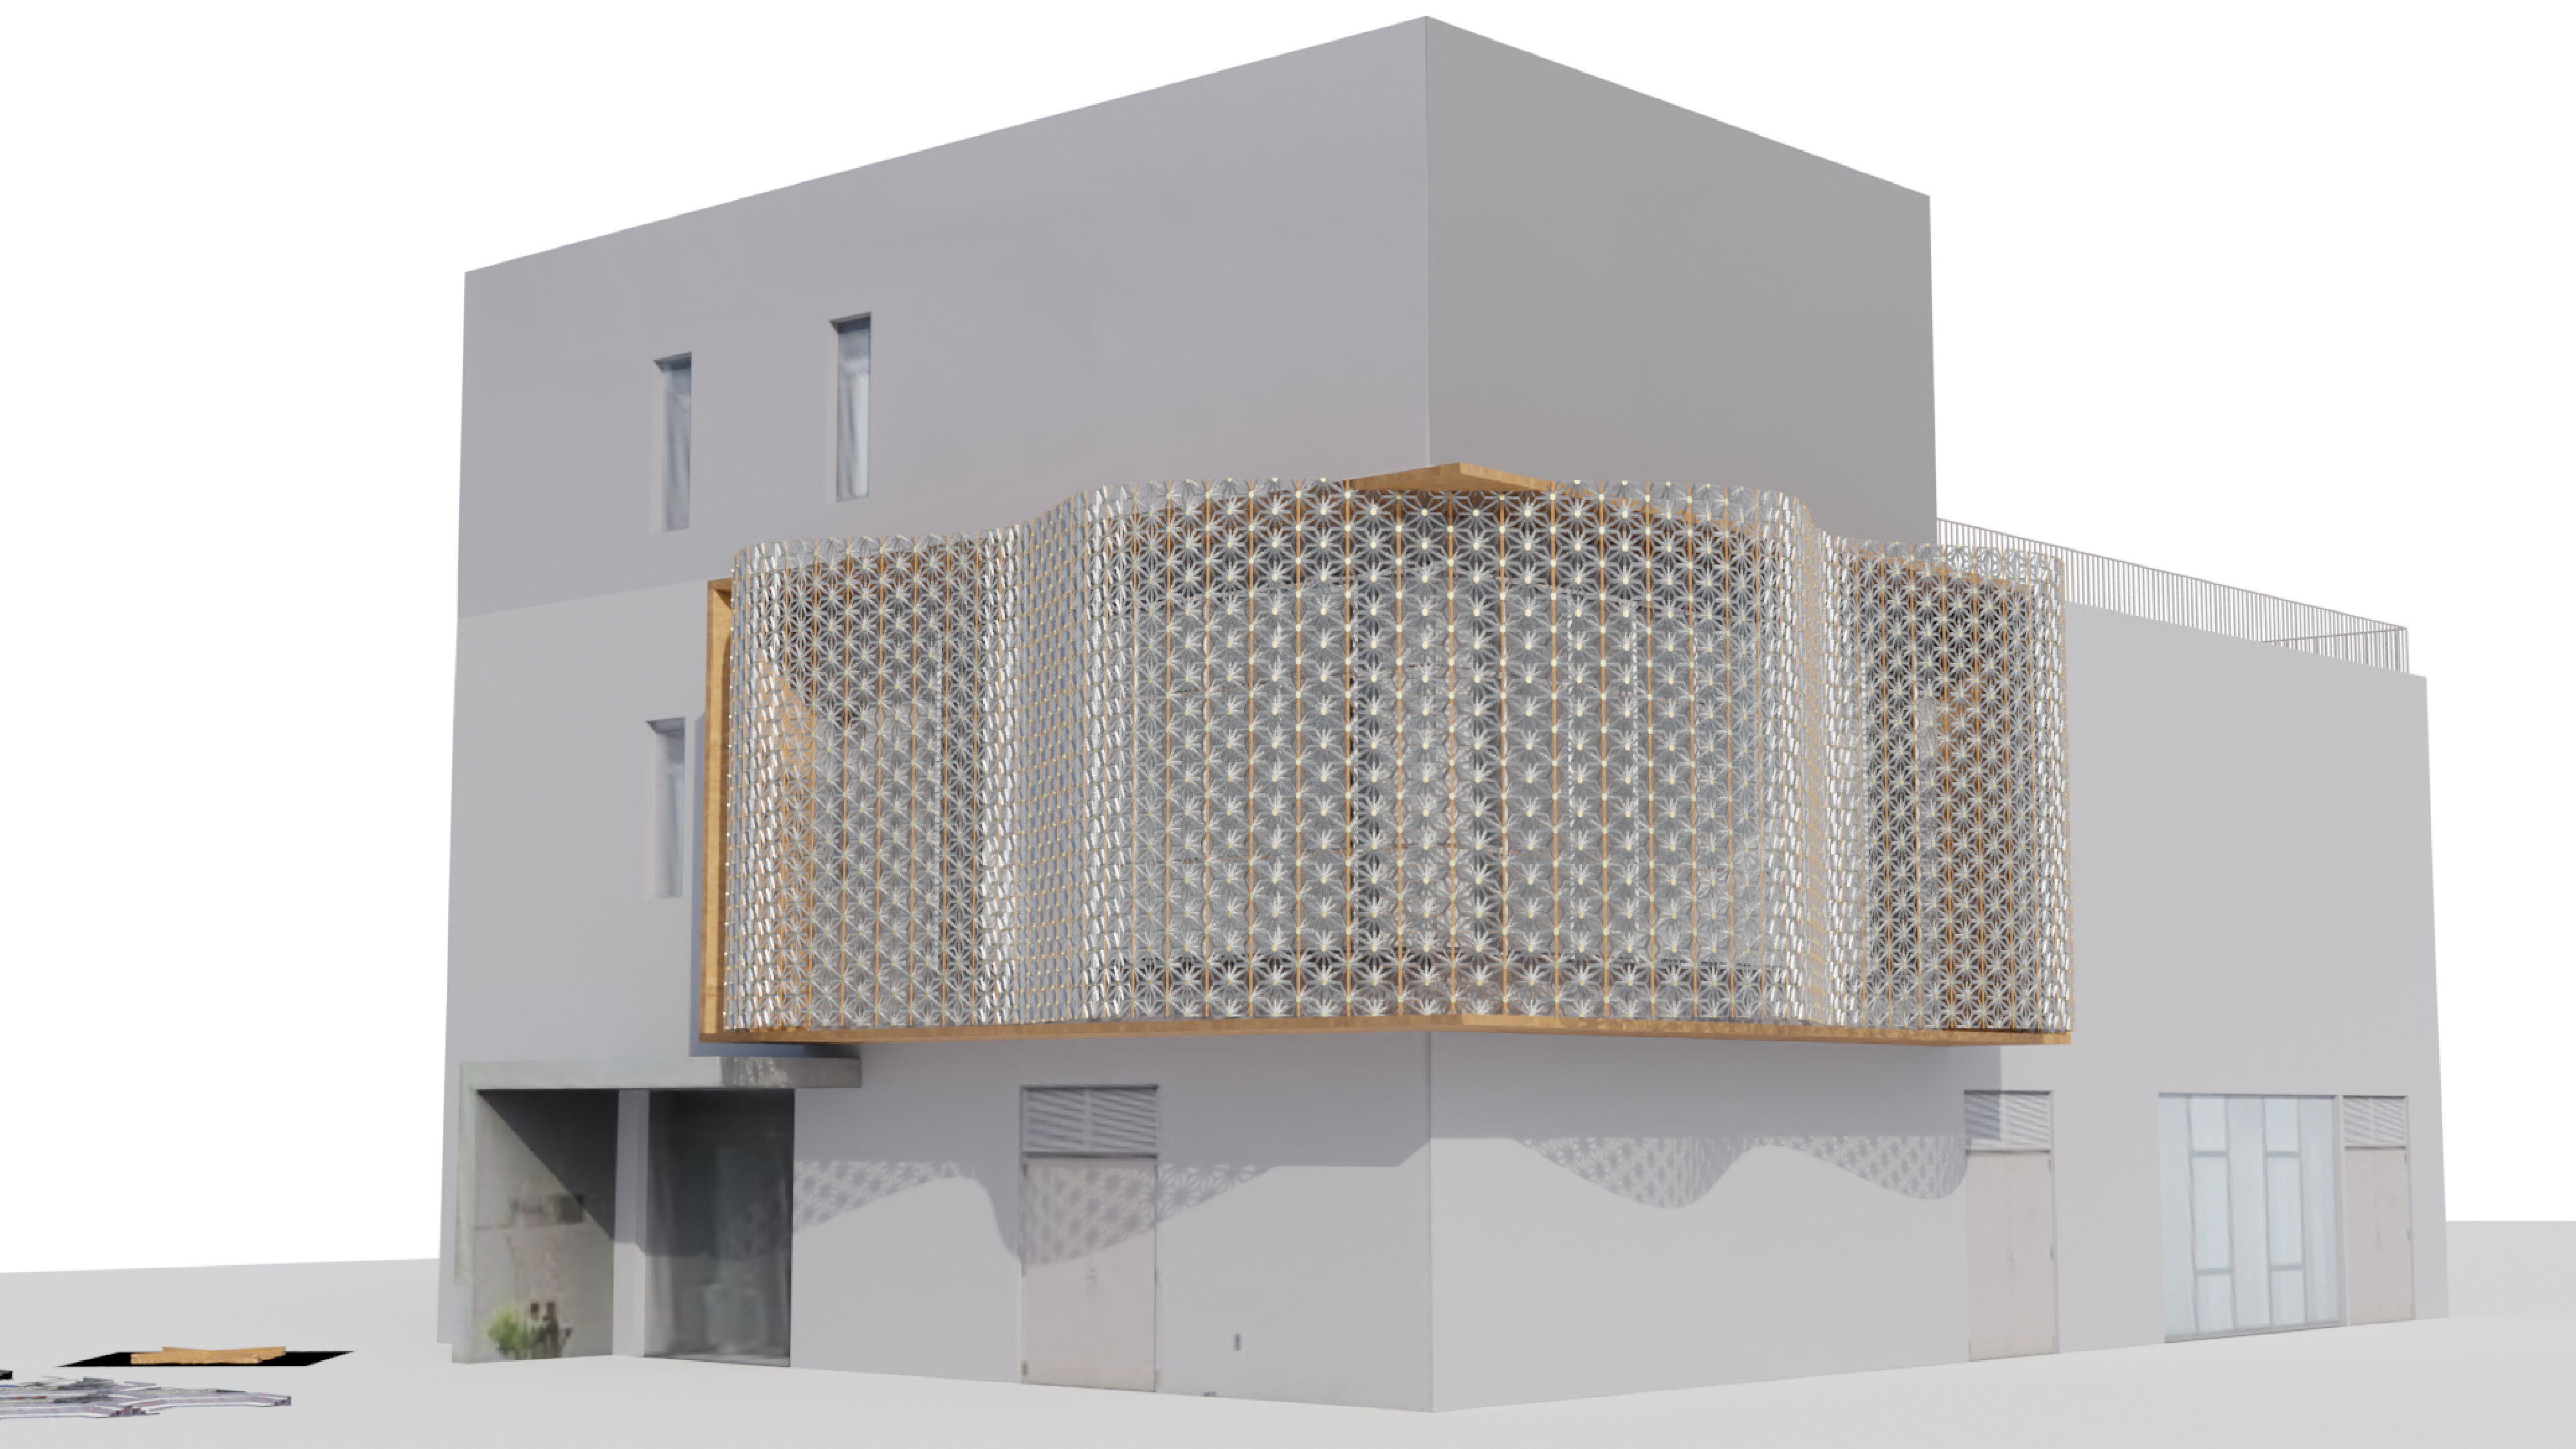
\includegraphics[width=1\linewidth]{Images/Pattern 3/0006}}\\
            \midrule
            \textit{Level 7} &  &  &
            \\
            {\includegraphics[width=1\linewidth]{Images/Wall 0/0007}} &
              {\includegraphics[width=1\linewidth]{Images/Pattern 1/0007}} &
              {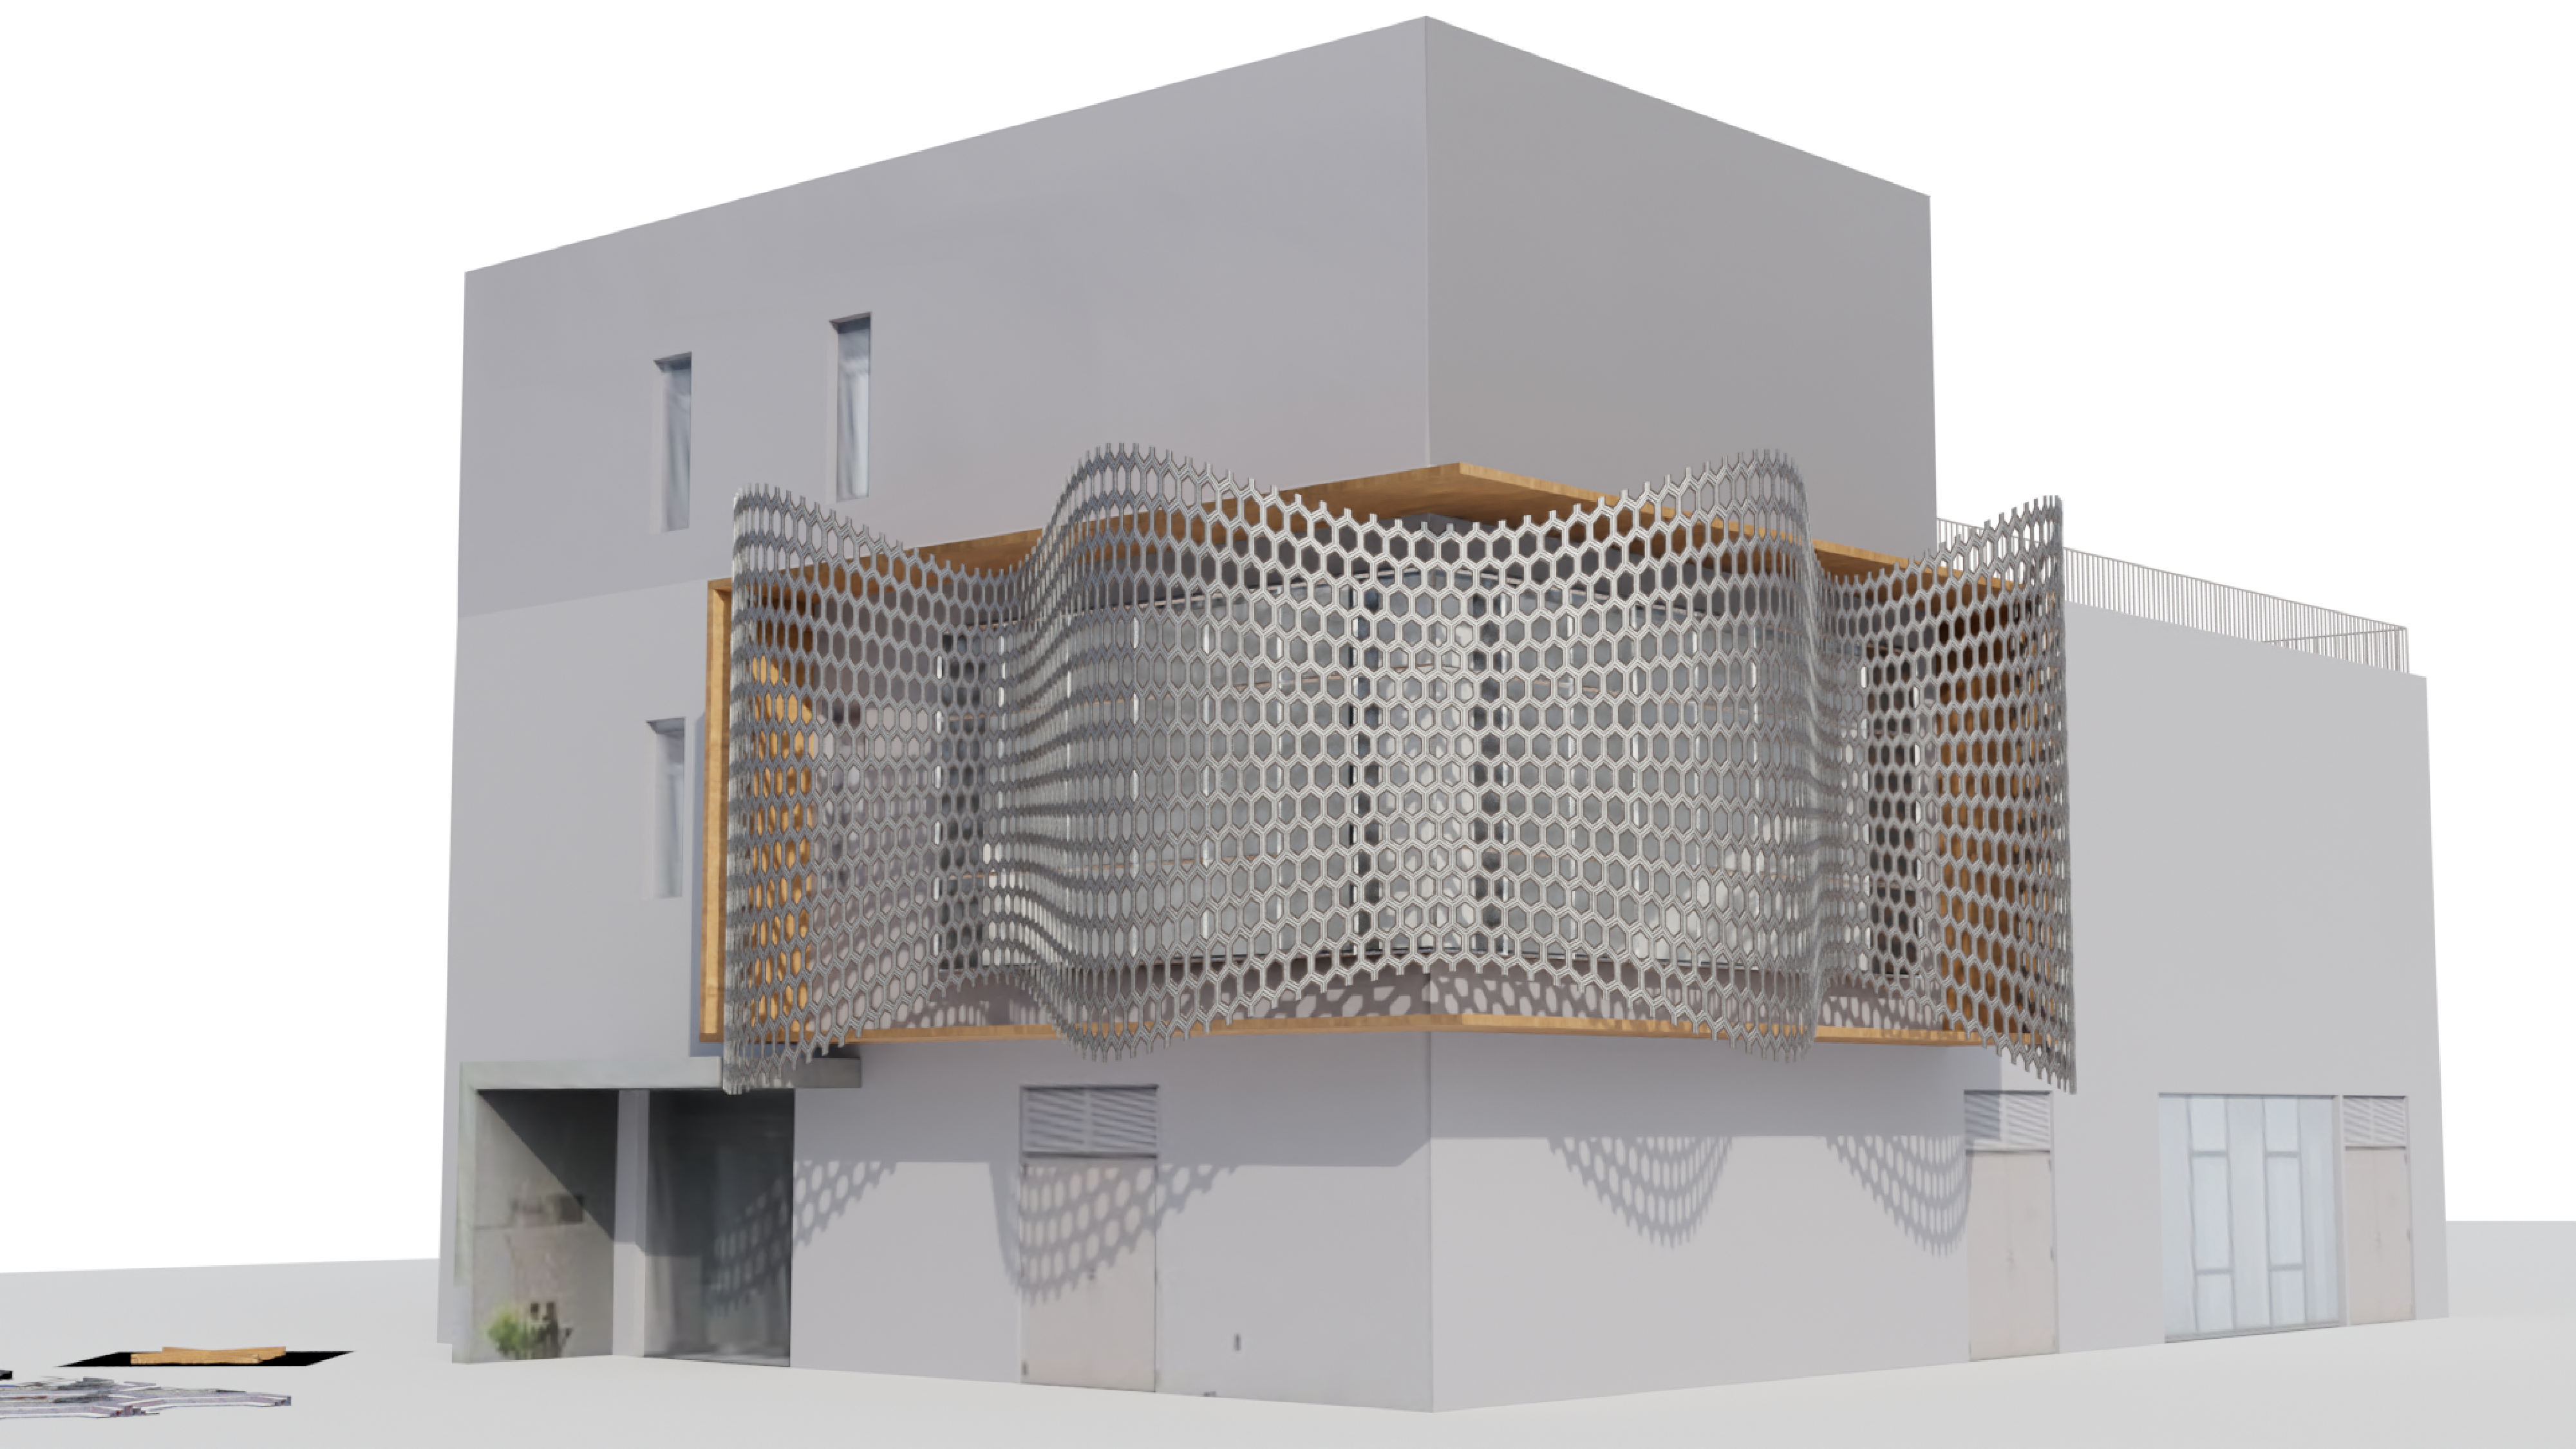
\includegraphics[width=1\linewidth]{Images/Pattern 2/0007}} &
              {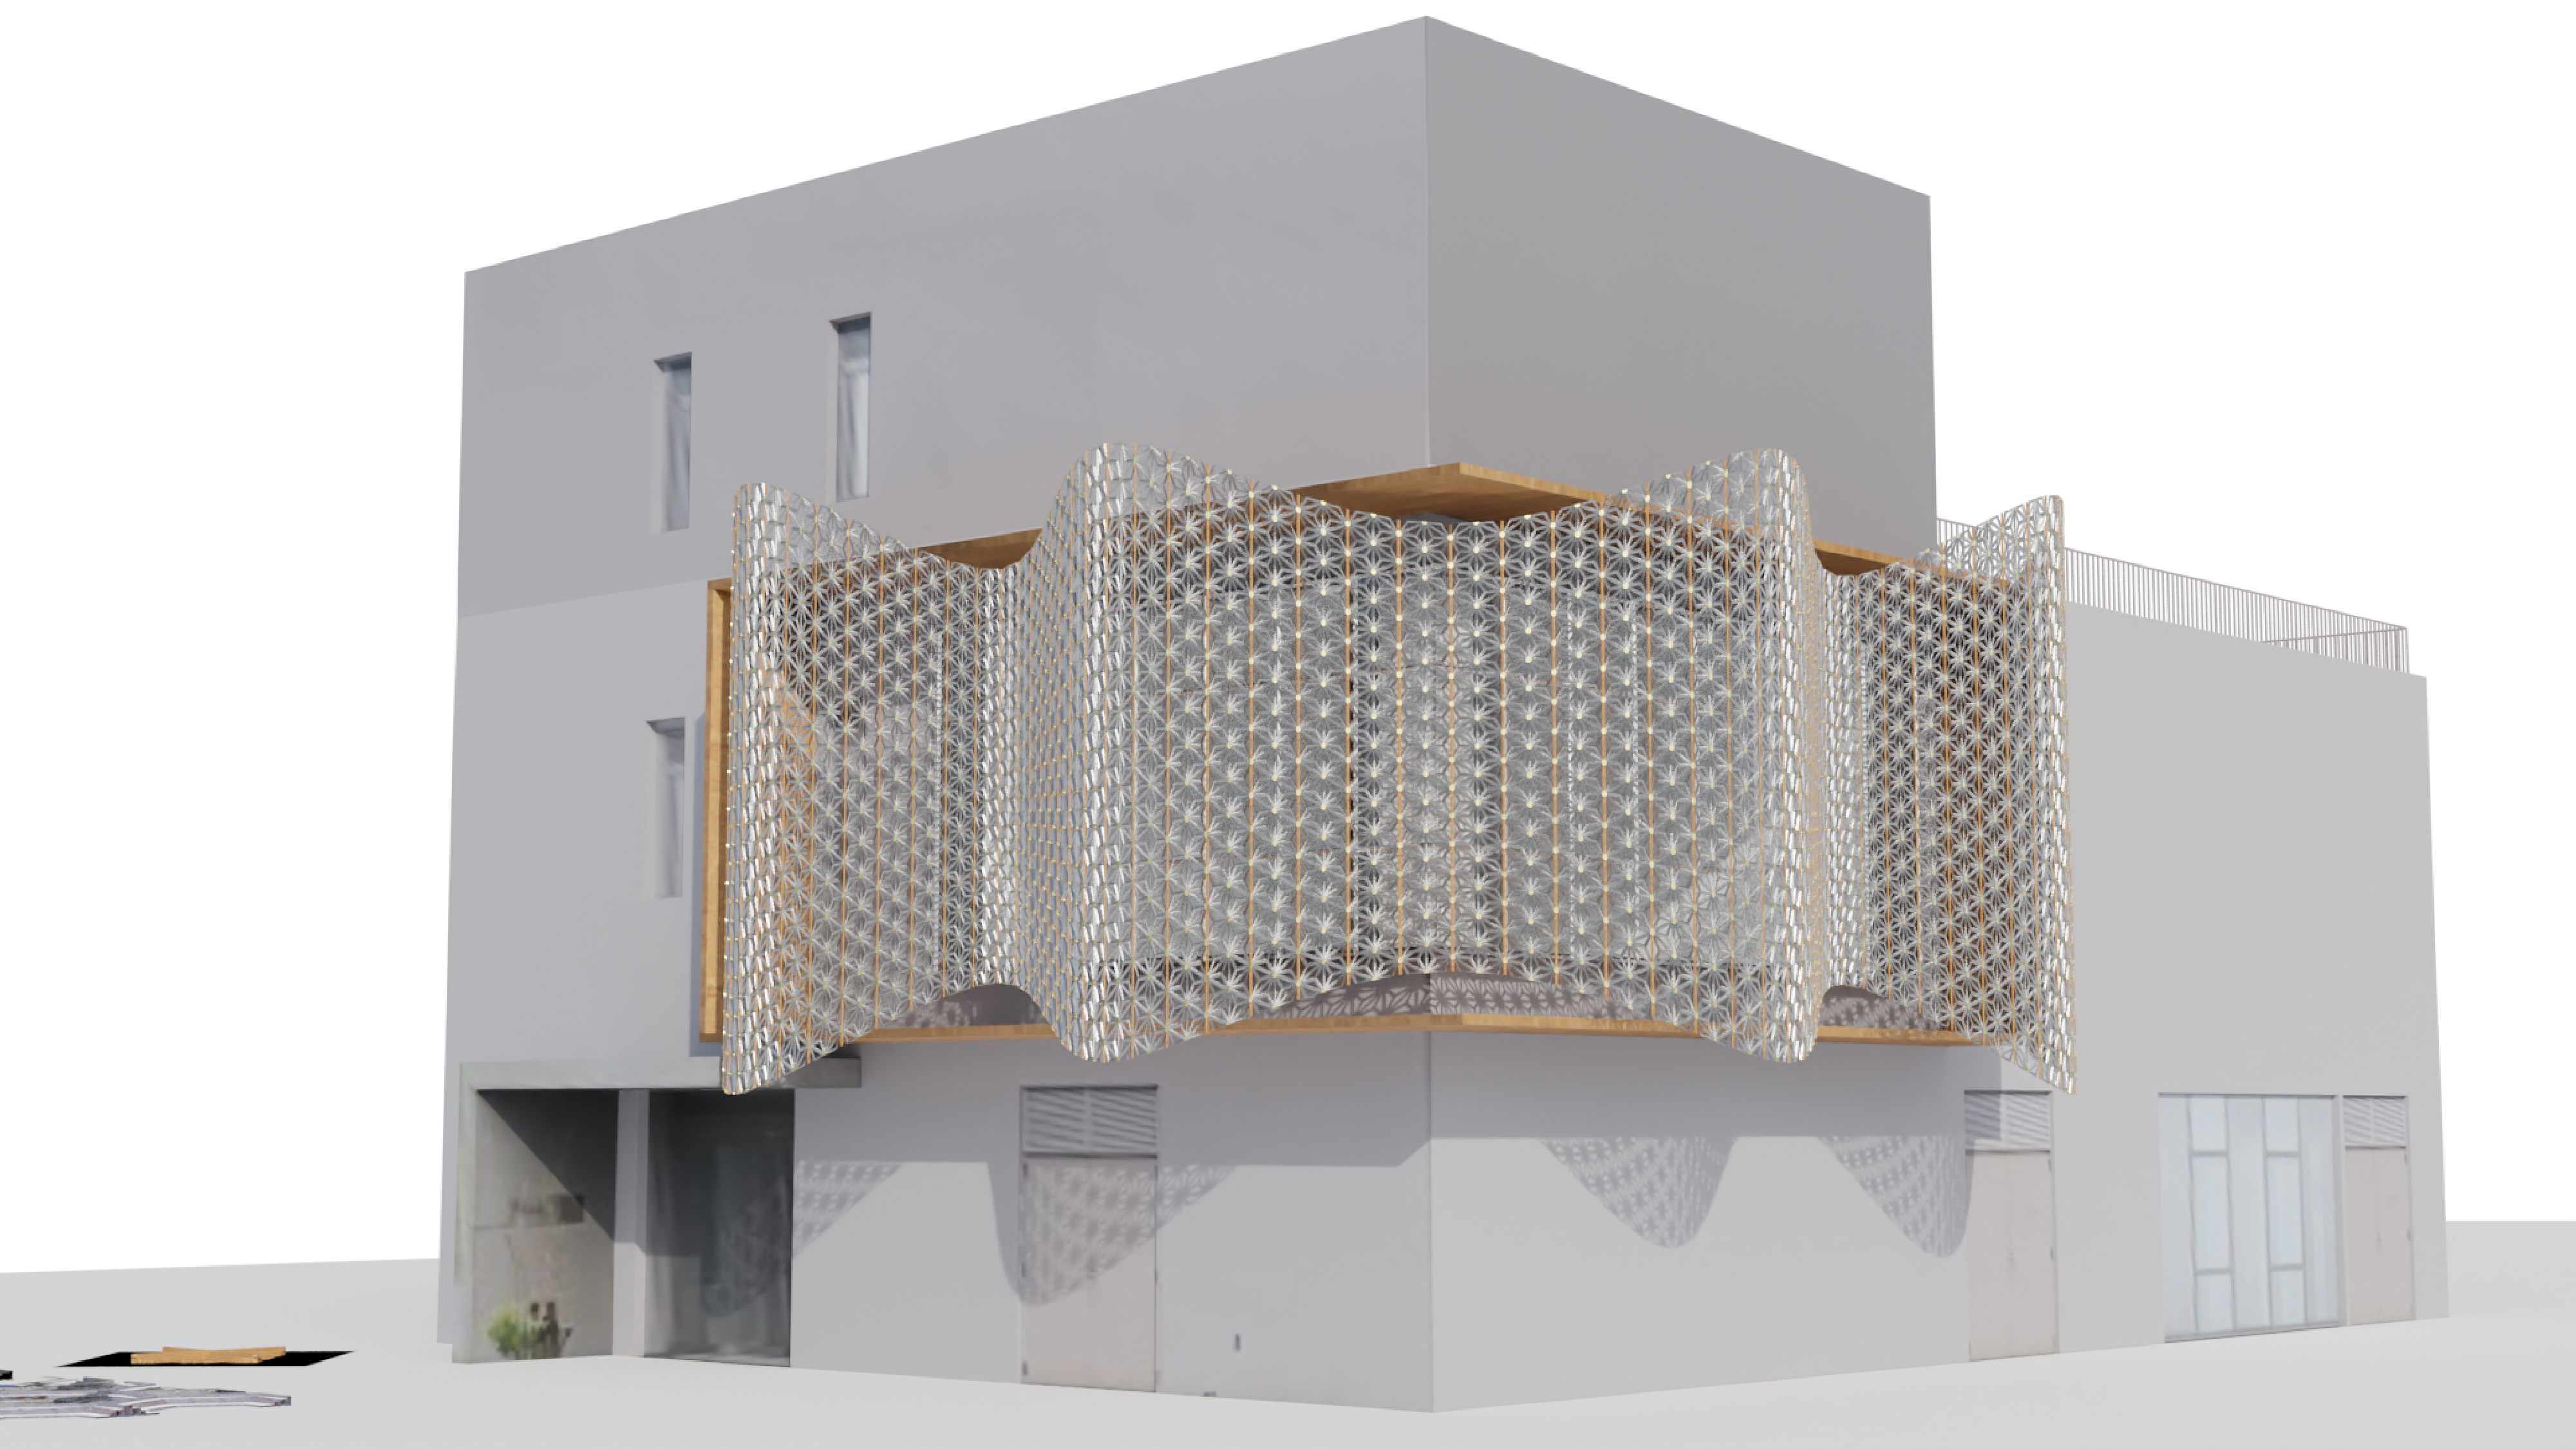
\includegraphics[width=1\linewidth]{Images/Pattern 3/0007}} \\
            \midrule
            \textit{Level 8} &  &  &
            \\
            {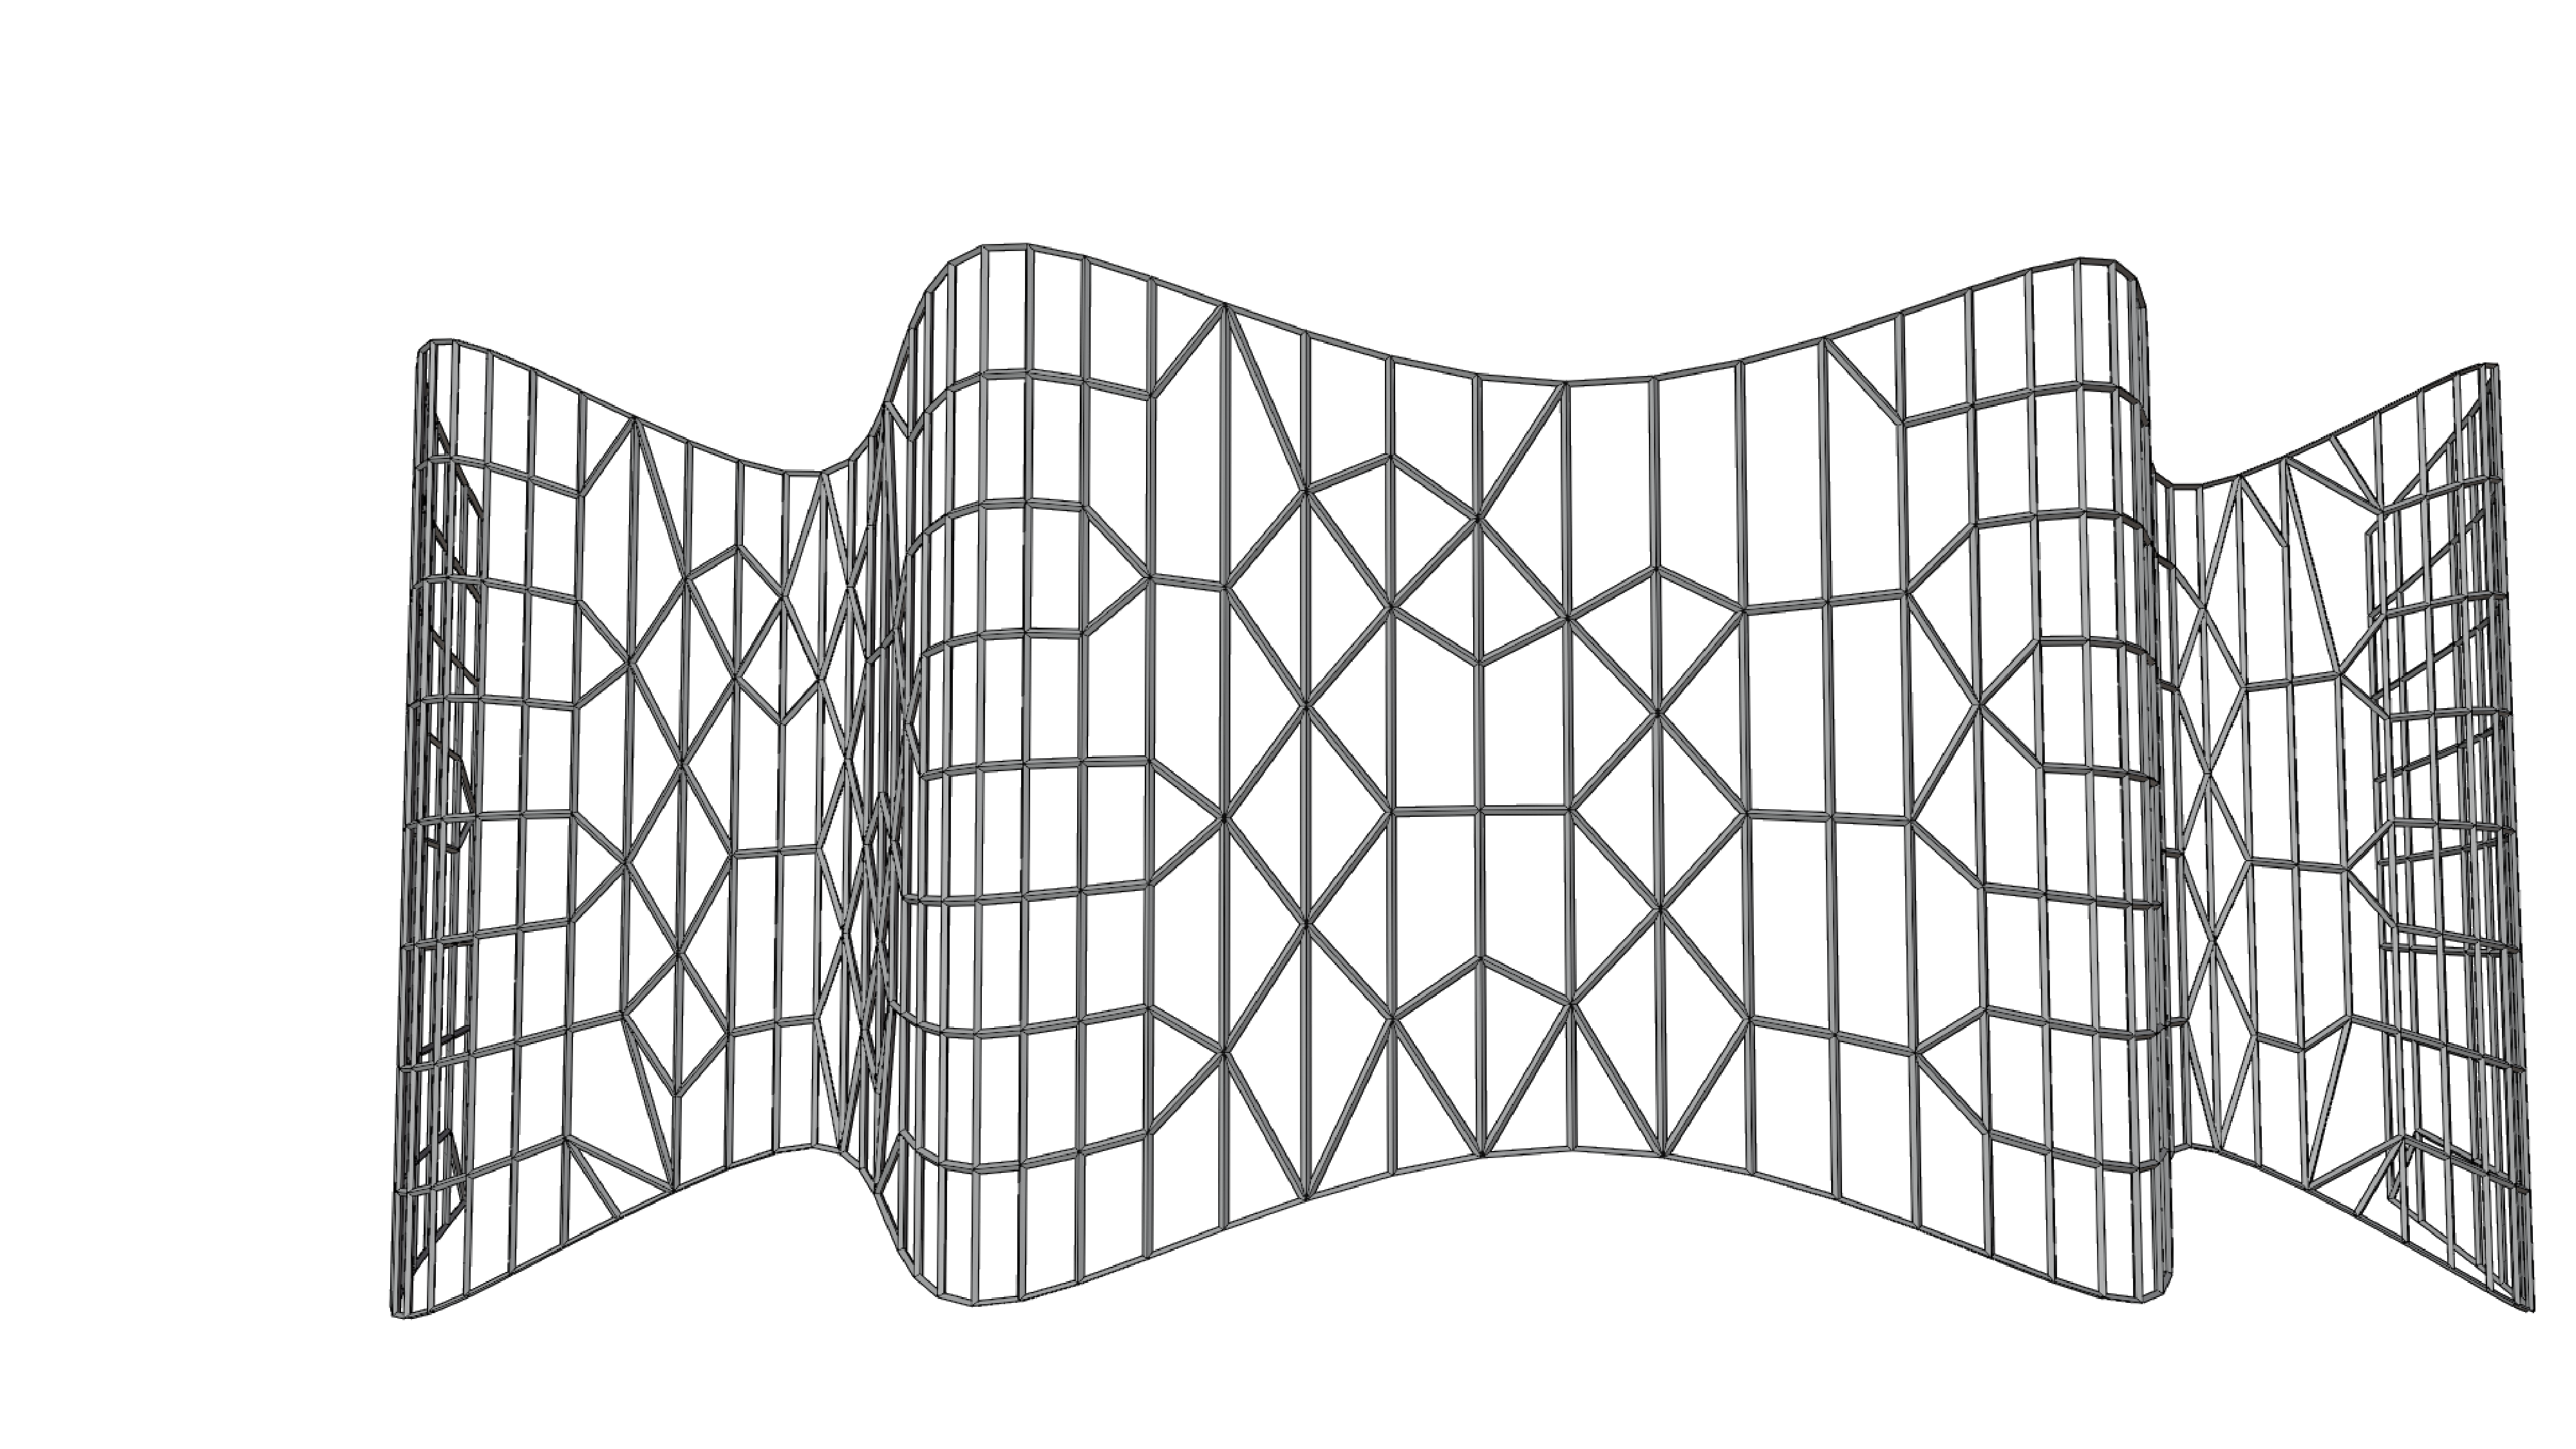
\includegraphics[width=1\linewidth]{Images/Wall 0/0008}} &
              {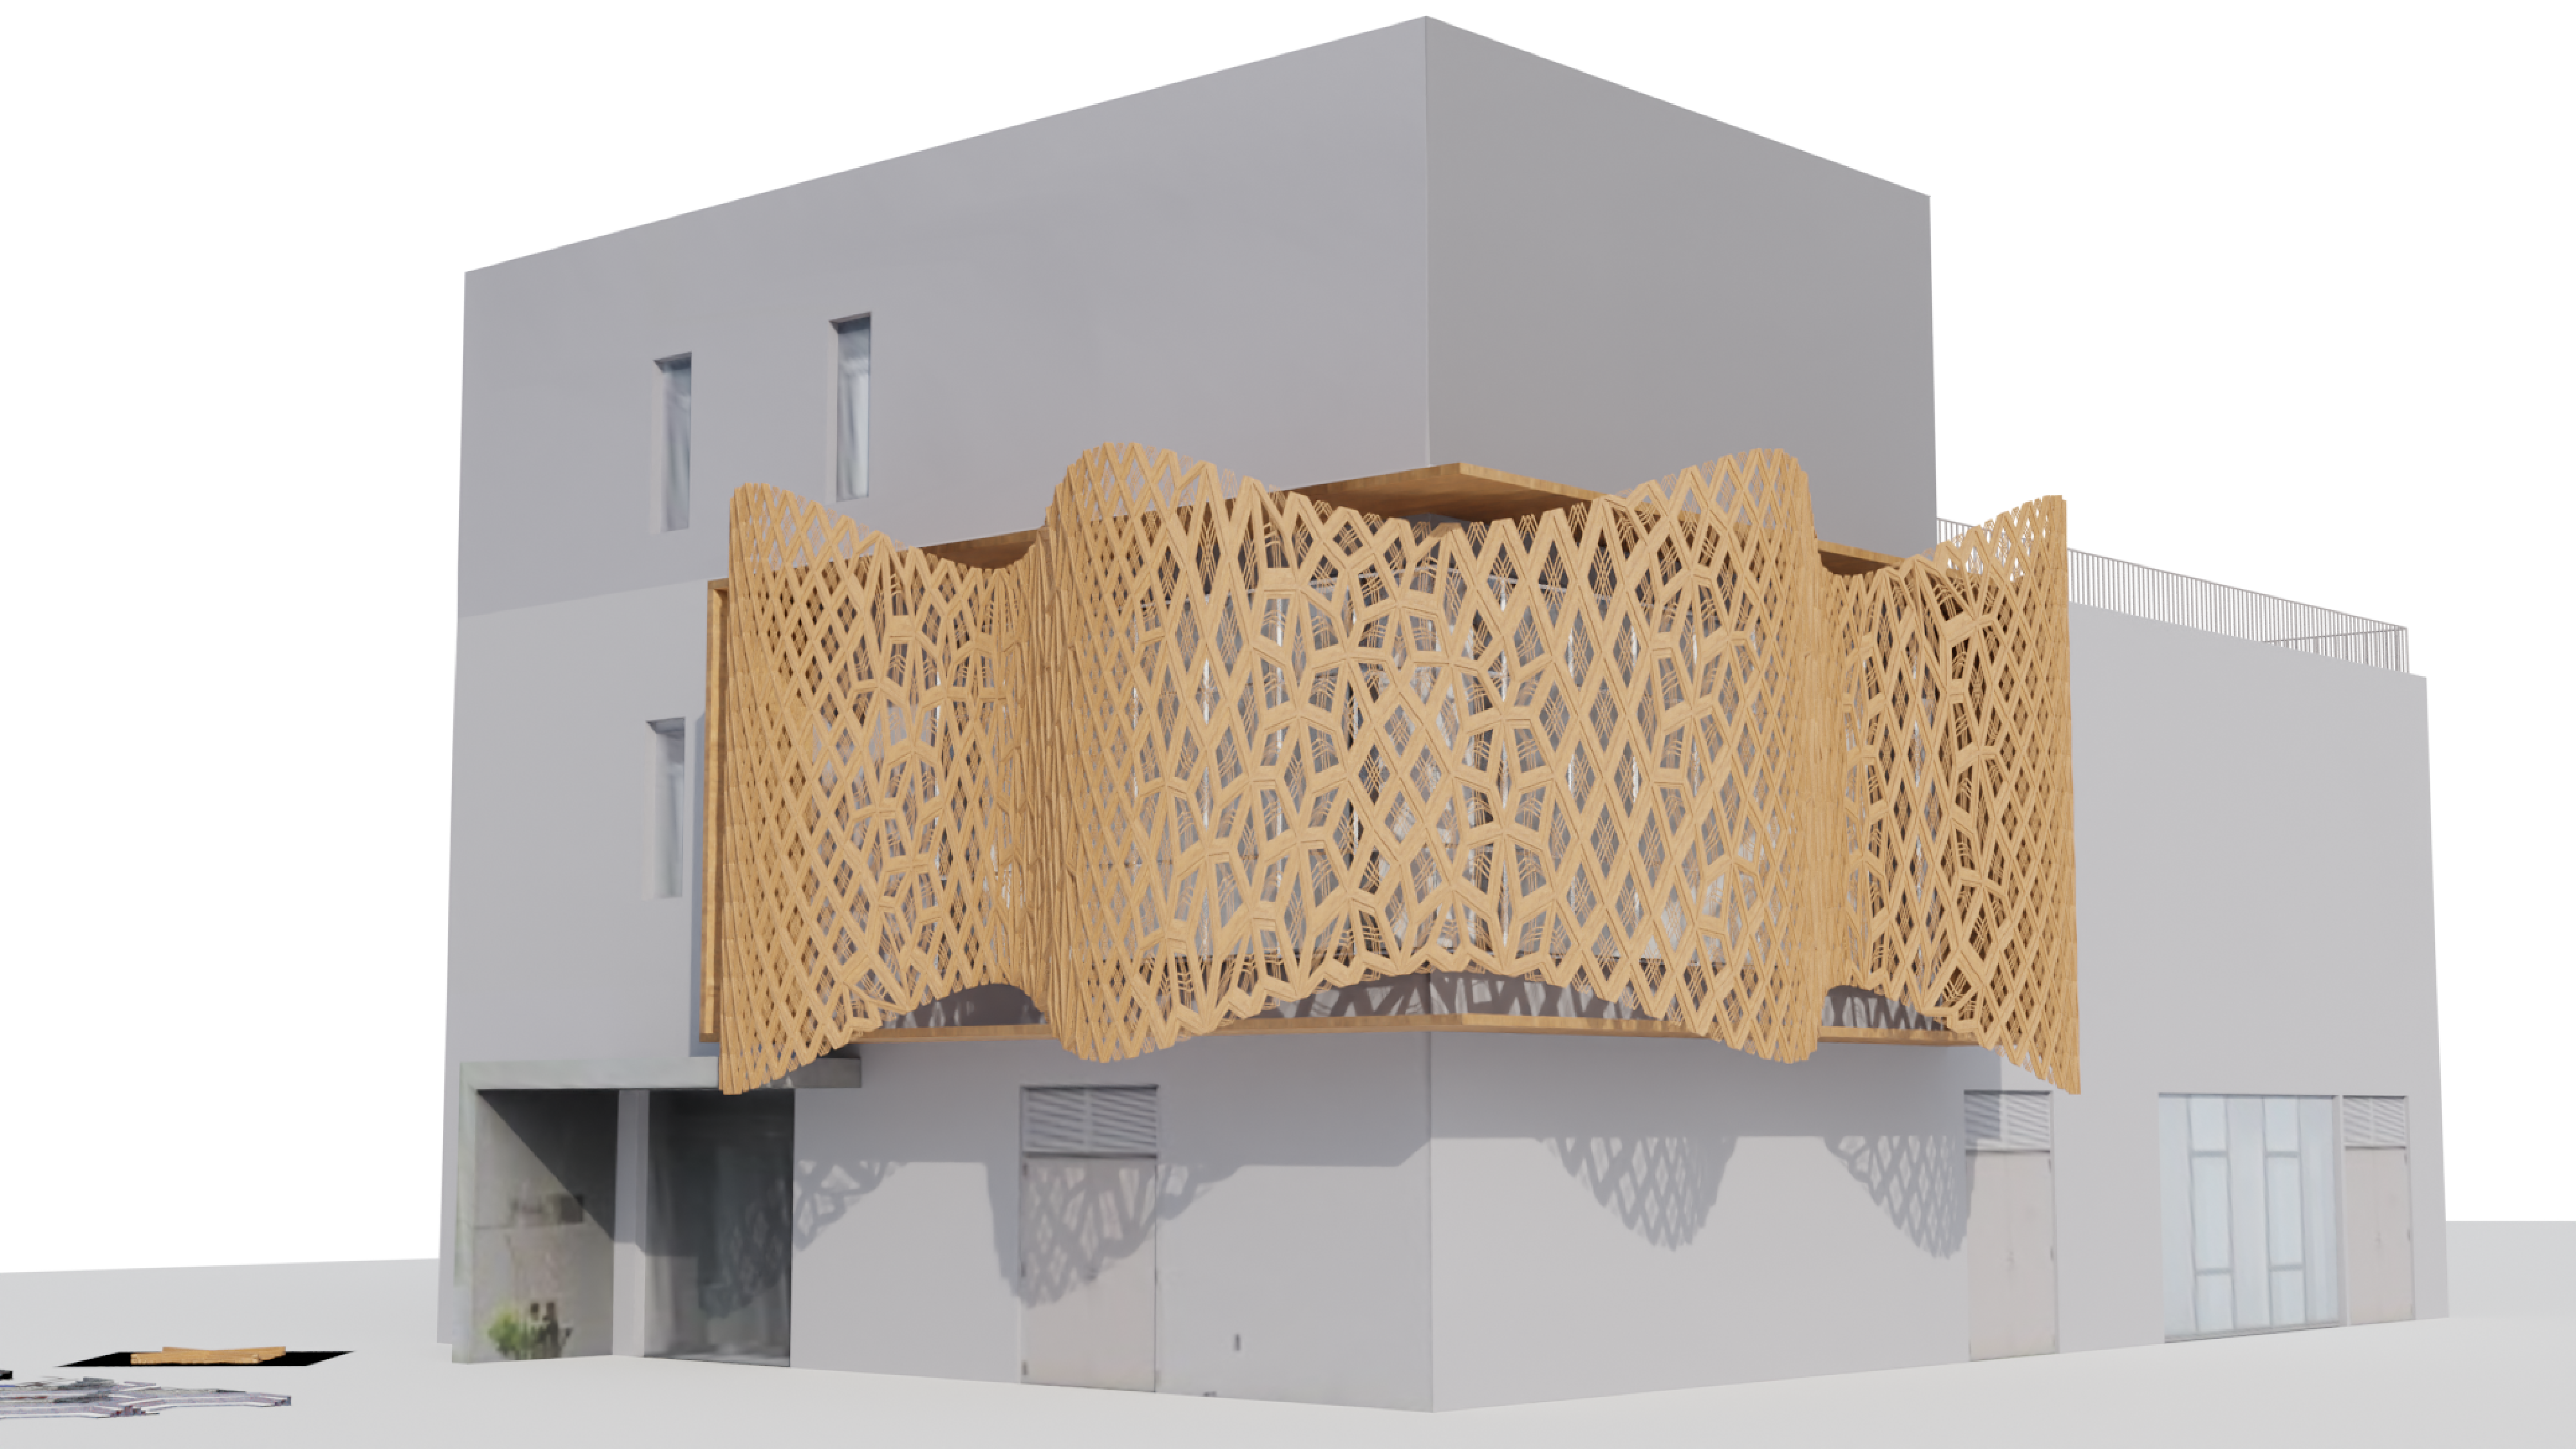
\includegraphics[width=1\linewidth]{Images/Pattern 1/0008}} &
              {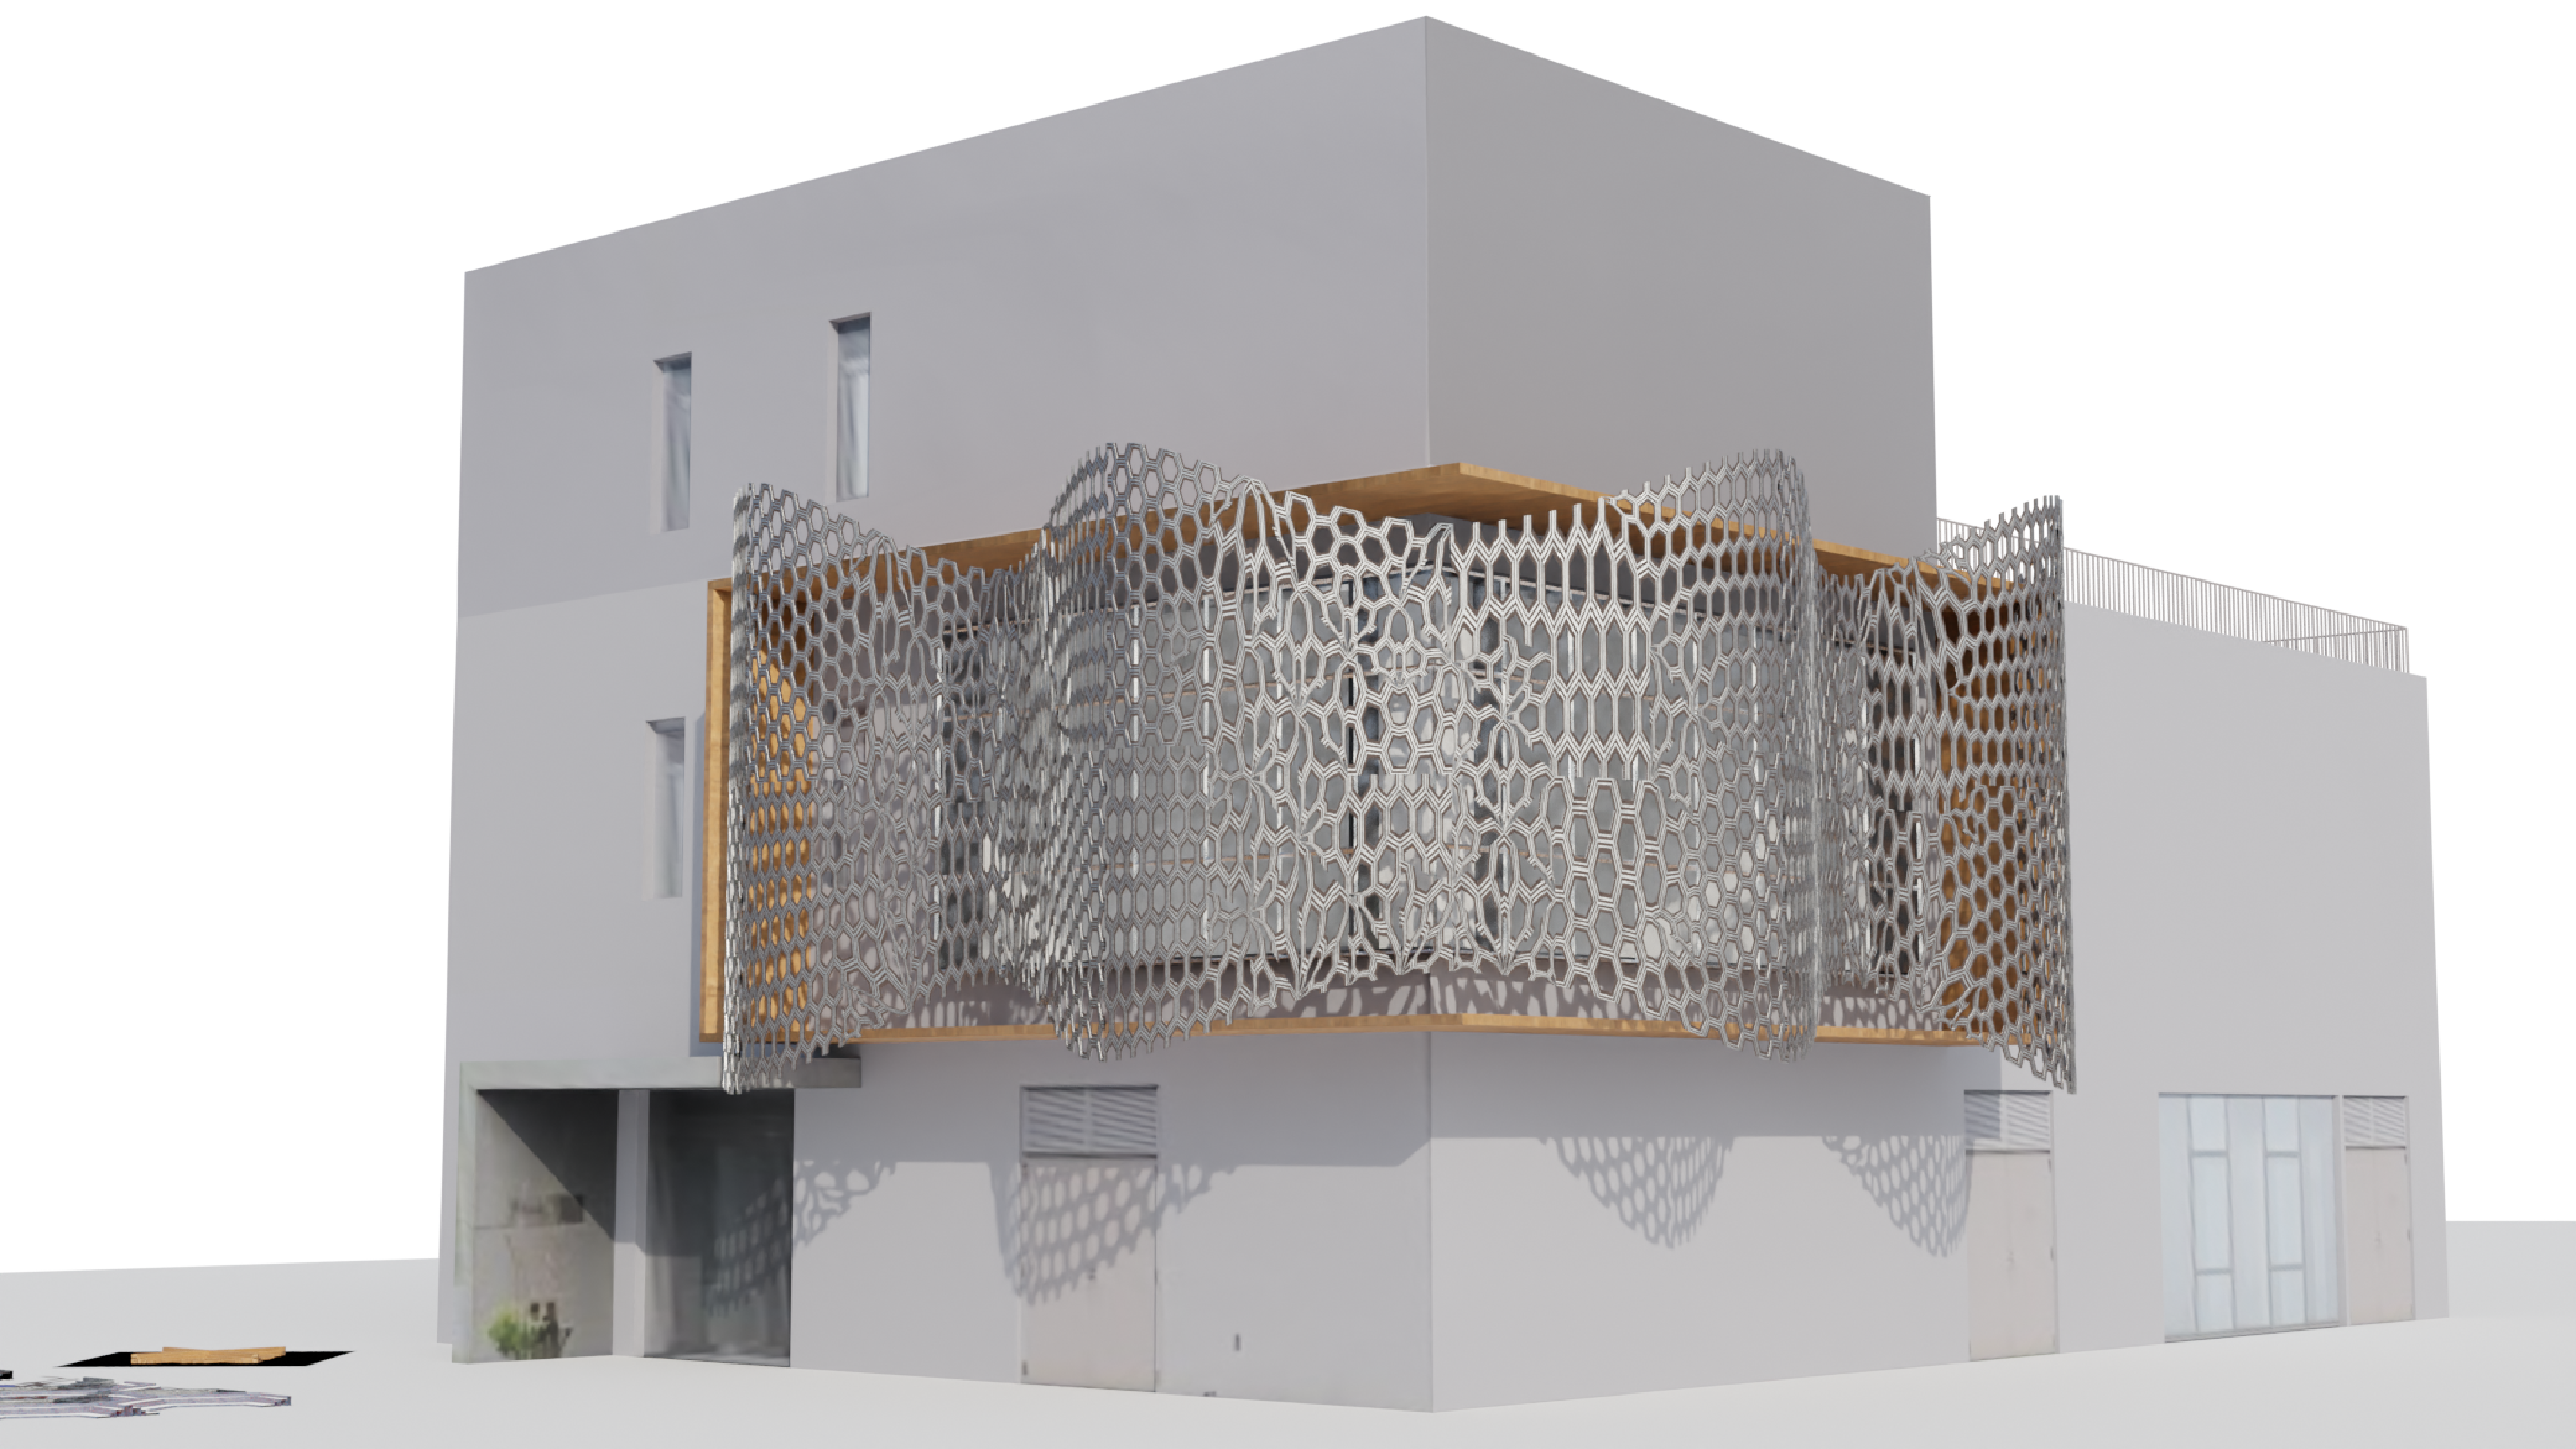
\includegraphics[width=1\linewidth]{Images/Pattern 2/0008}} &
              {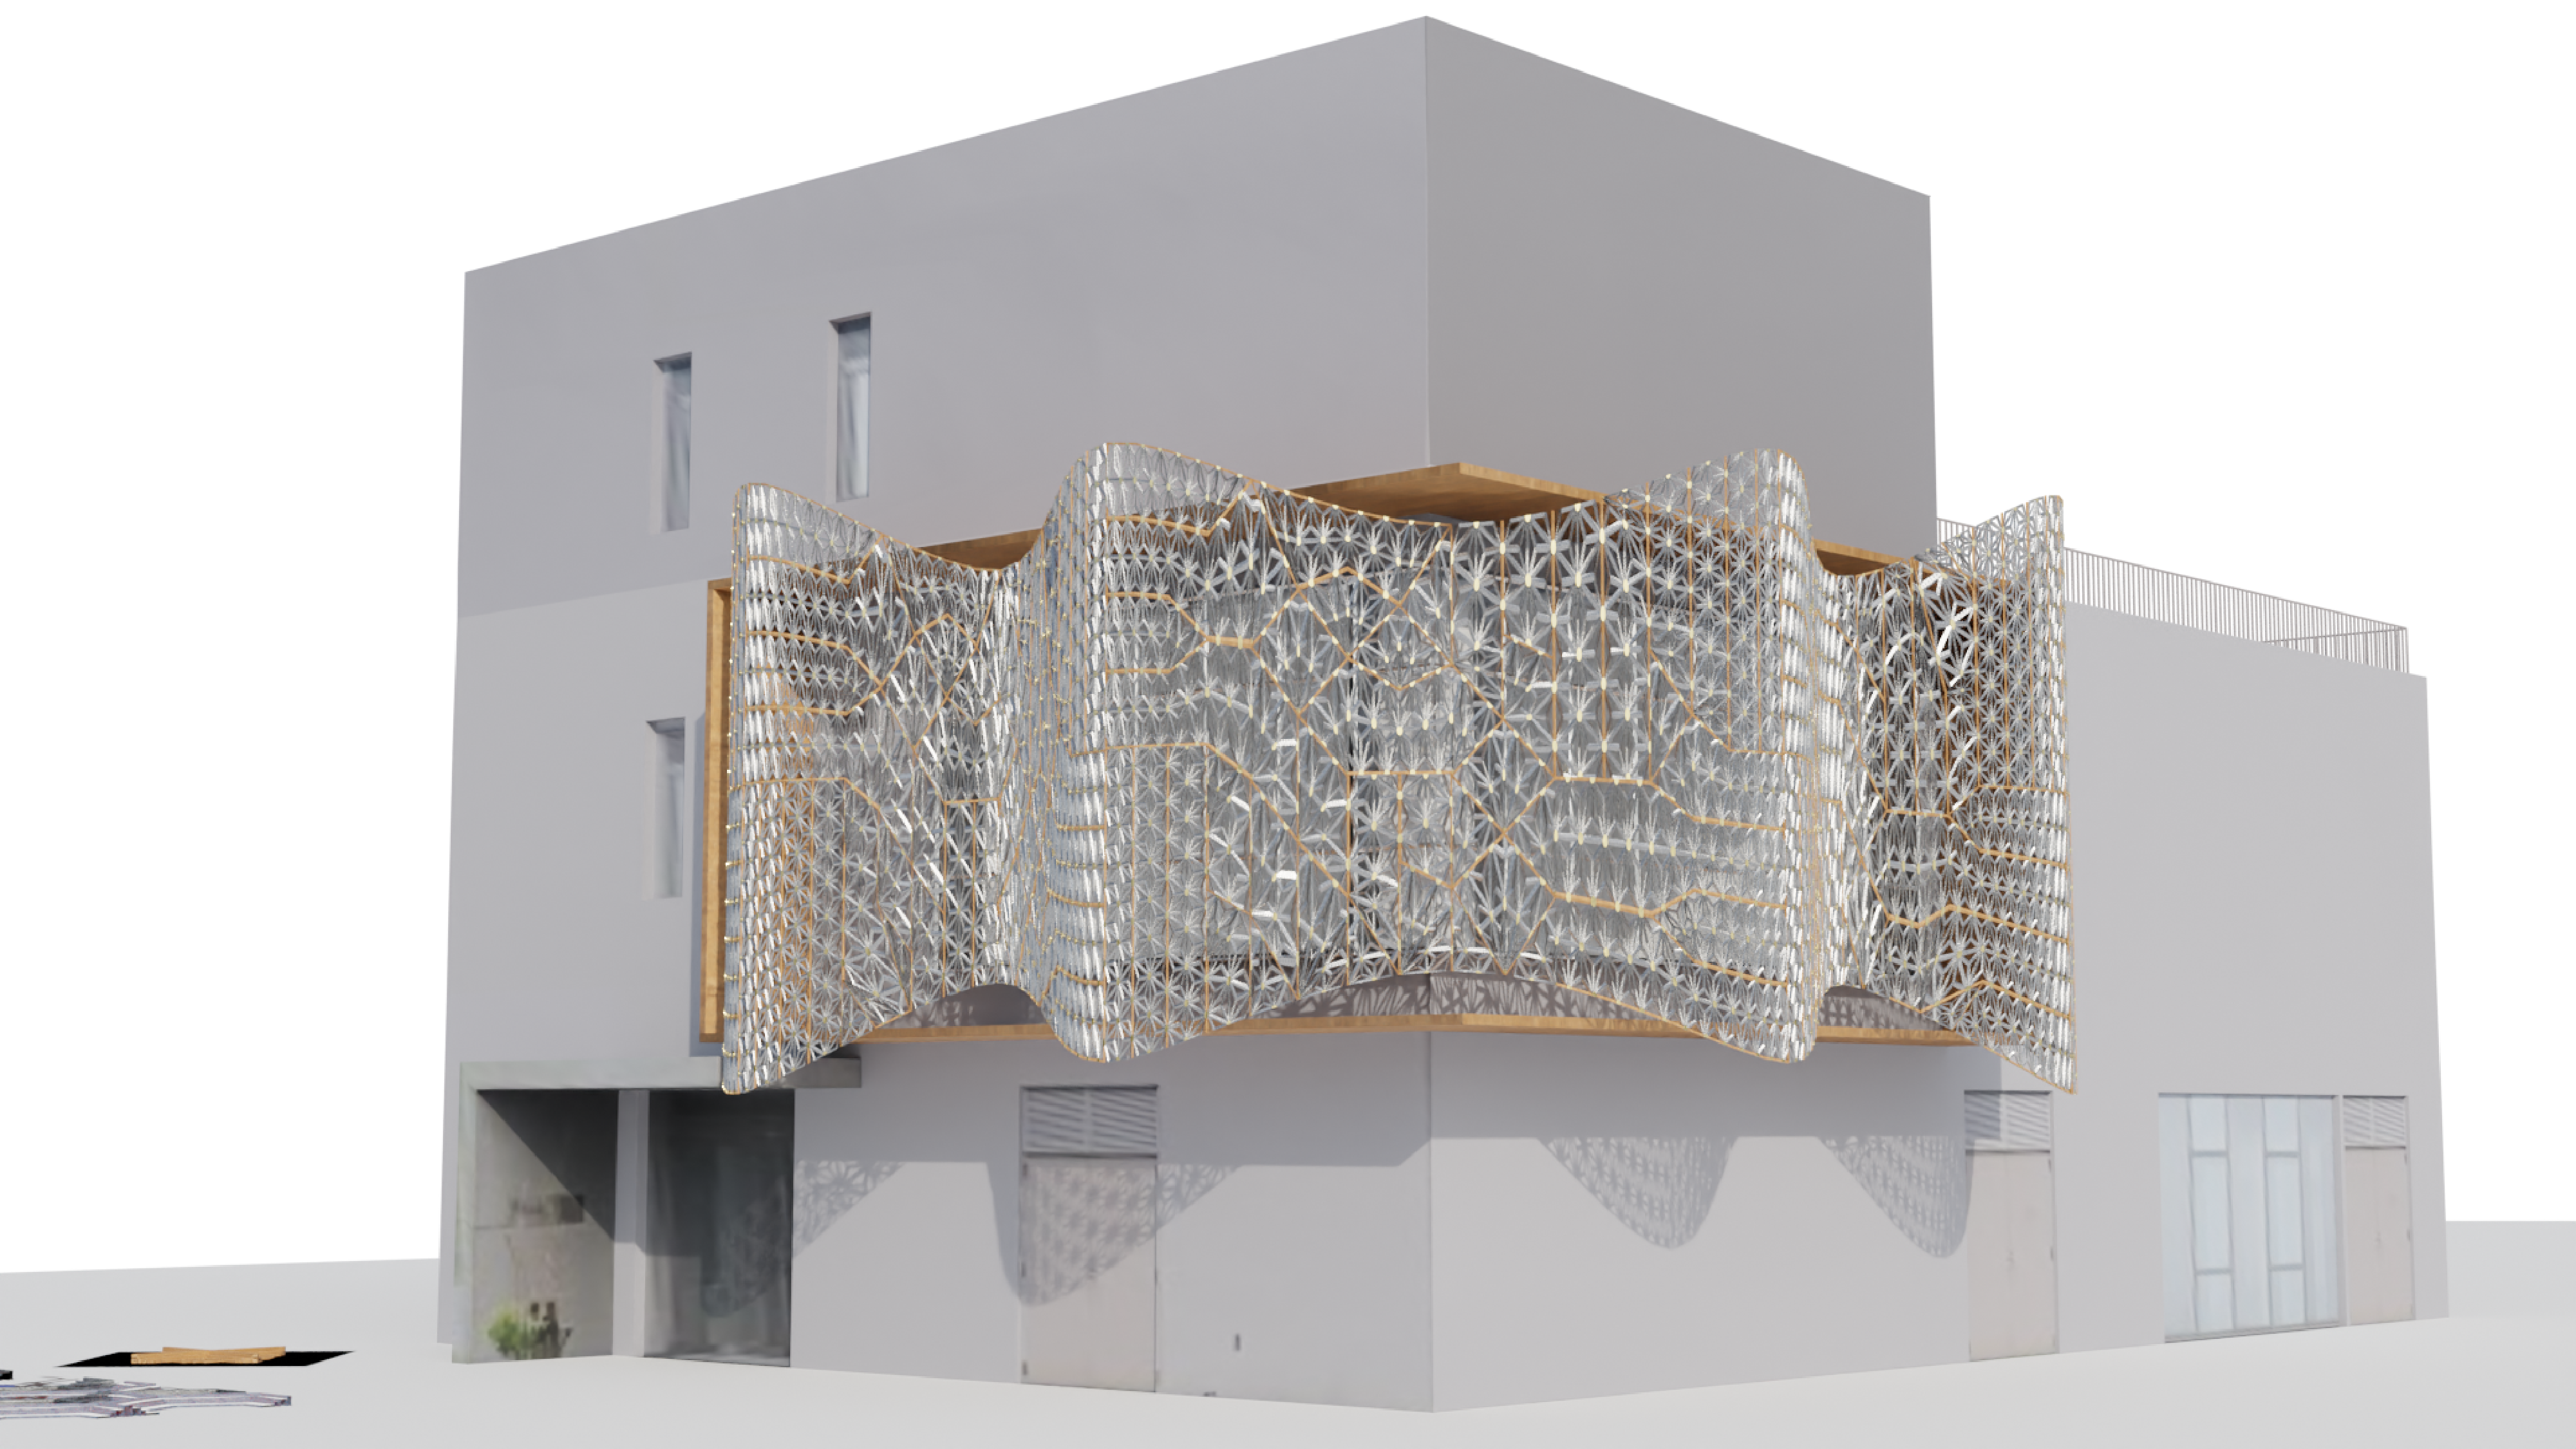
\includegraphics[width=1\linewidth]{Images/Pattern 3/0008}}\\
            \midrule
            \textit{Level 9} &  &  &
            \\
            {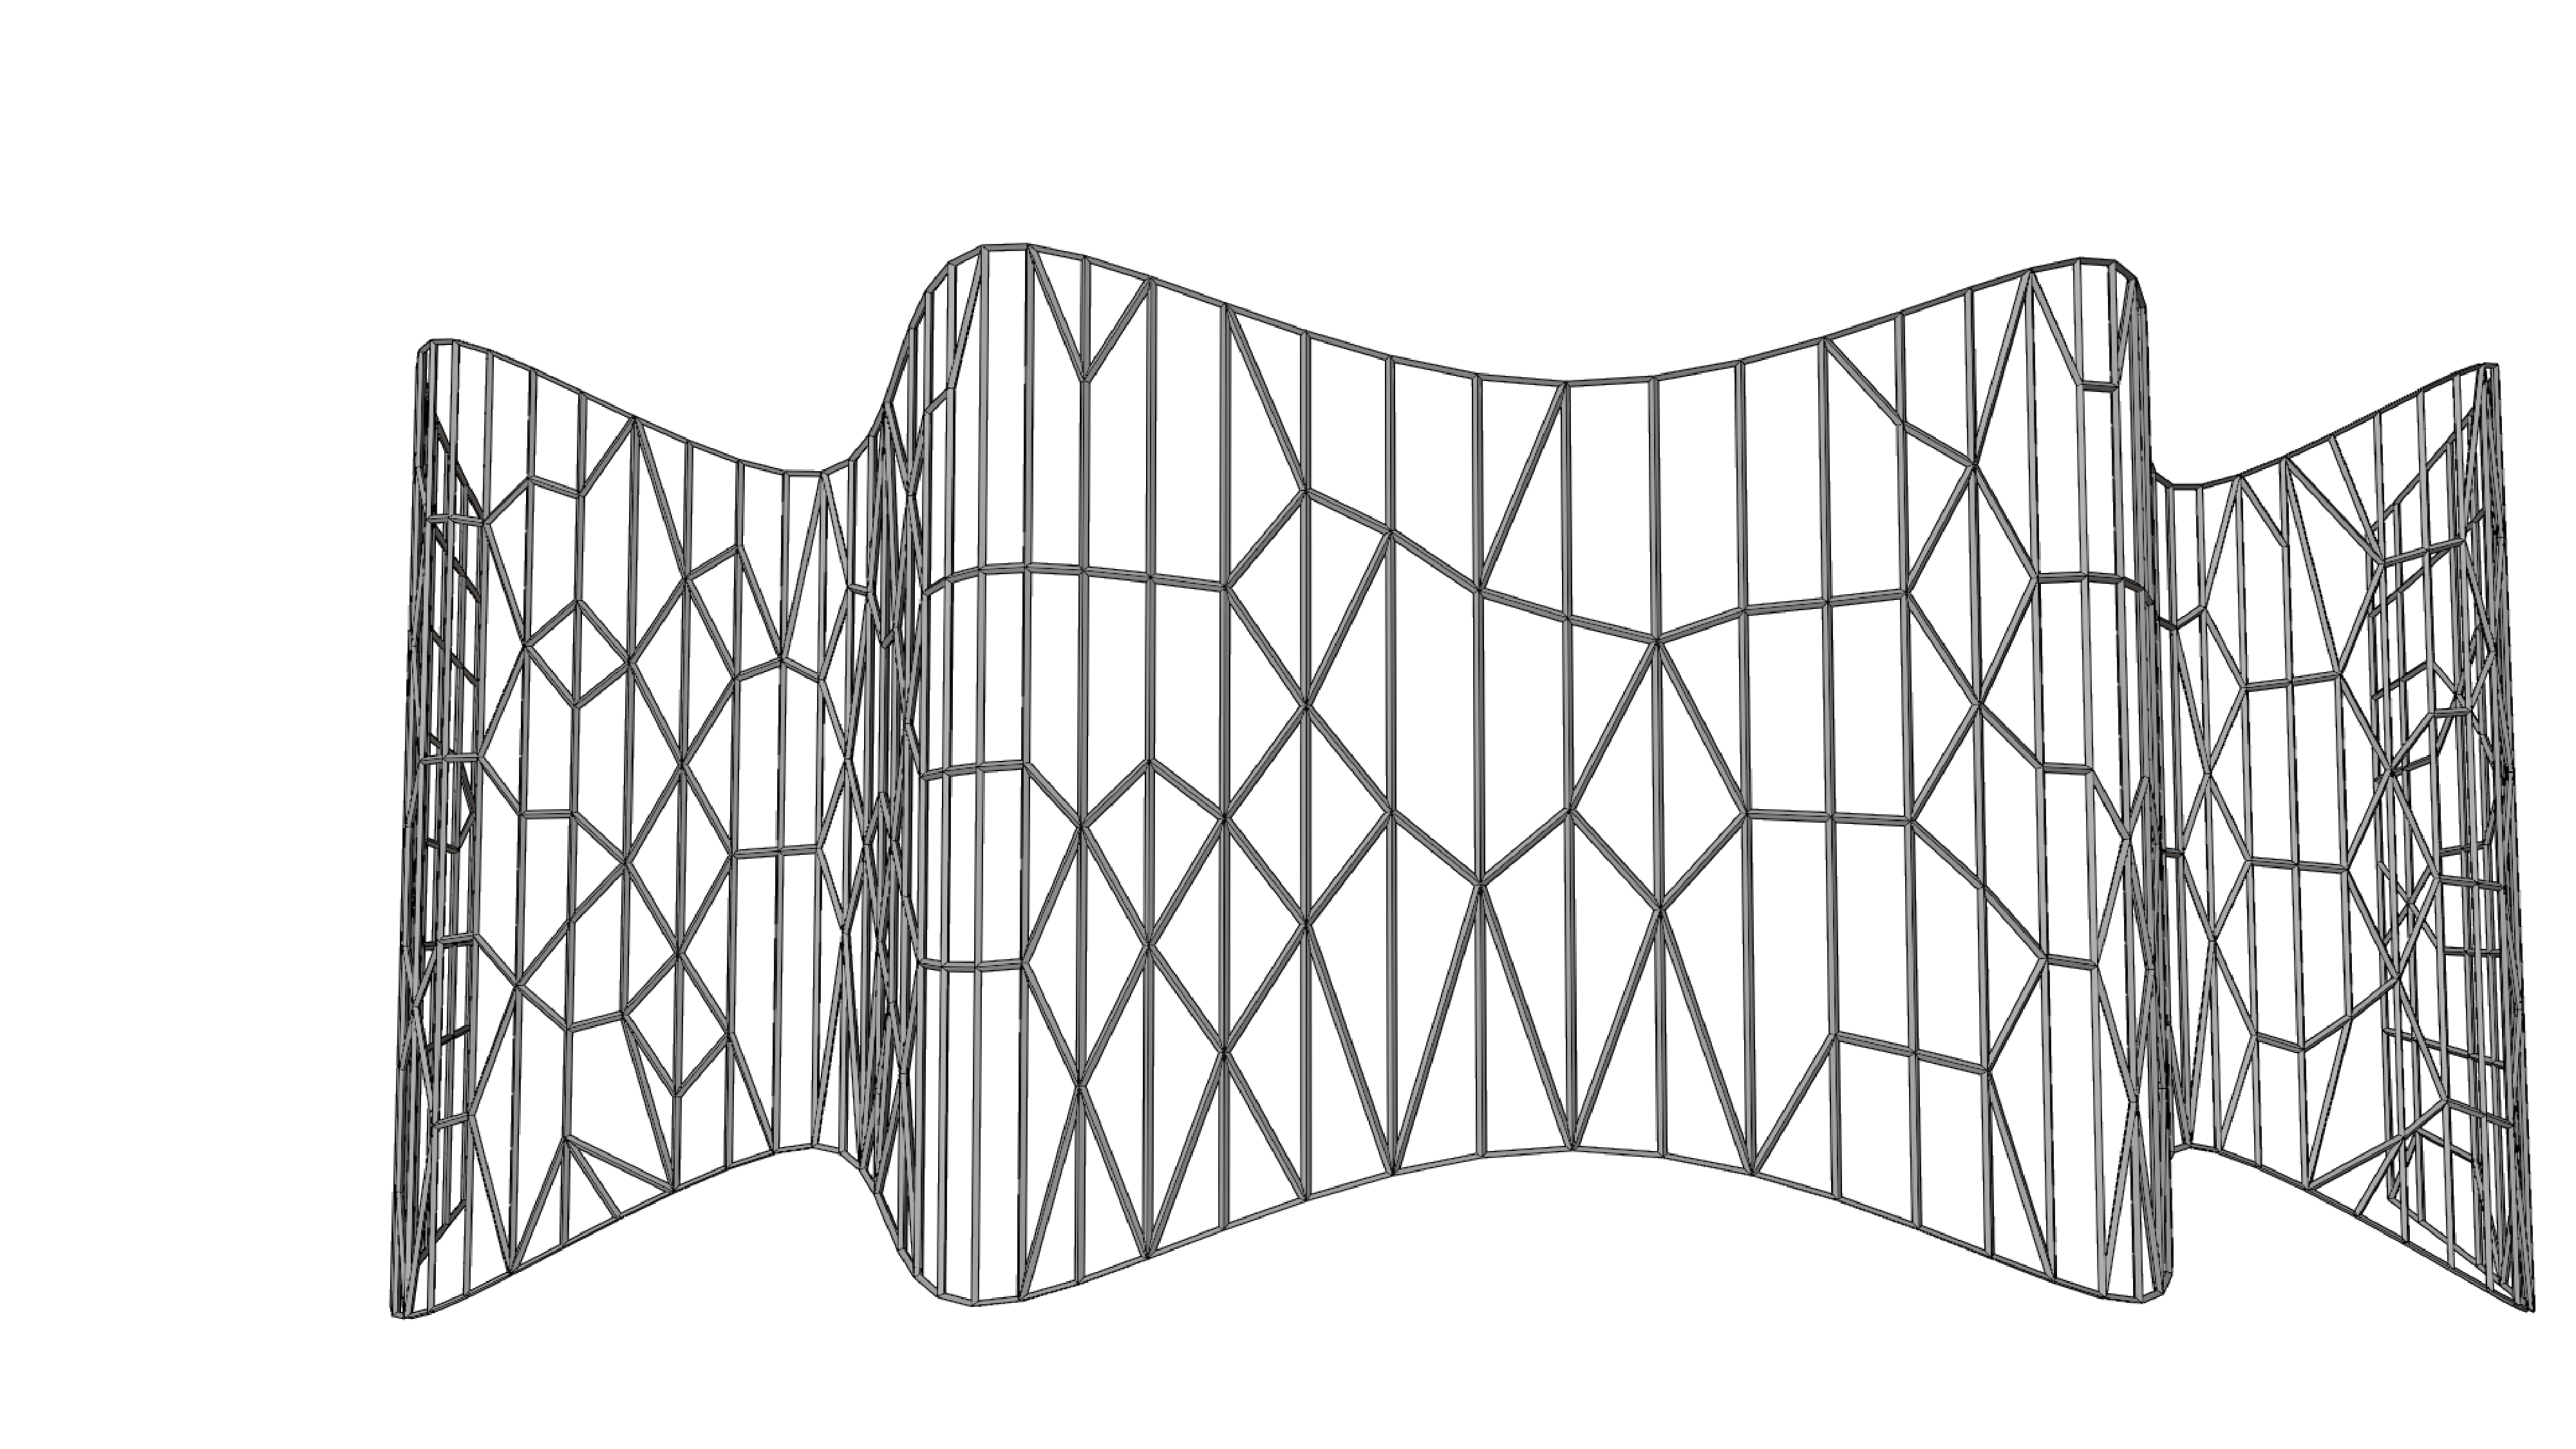
\includegraphics[width=1\linewidth]{Images/Wall 0/0009}} &
              {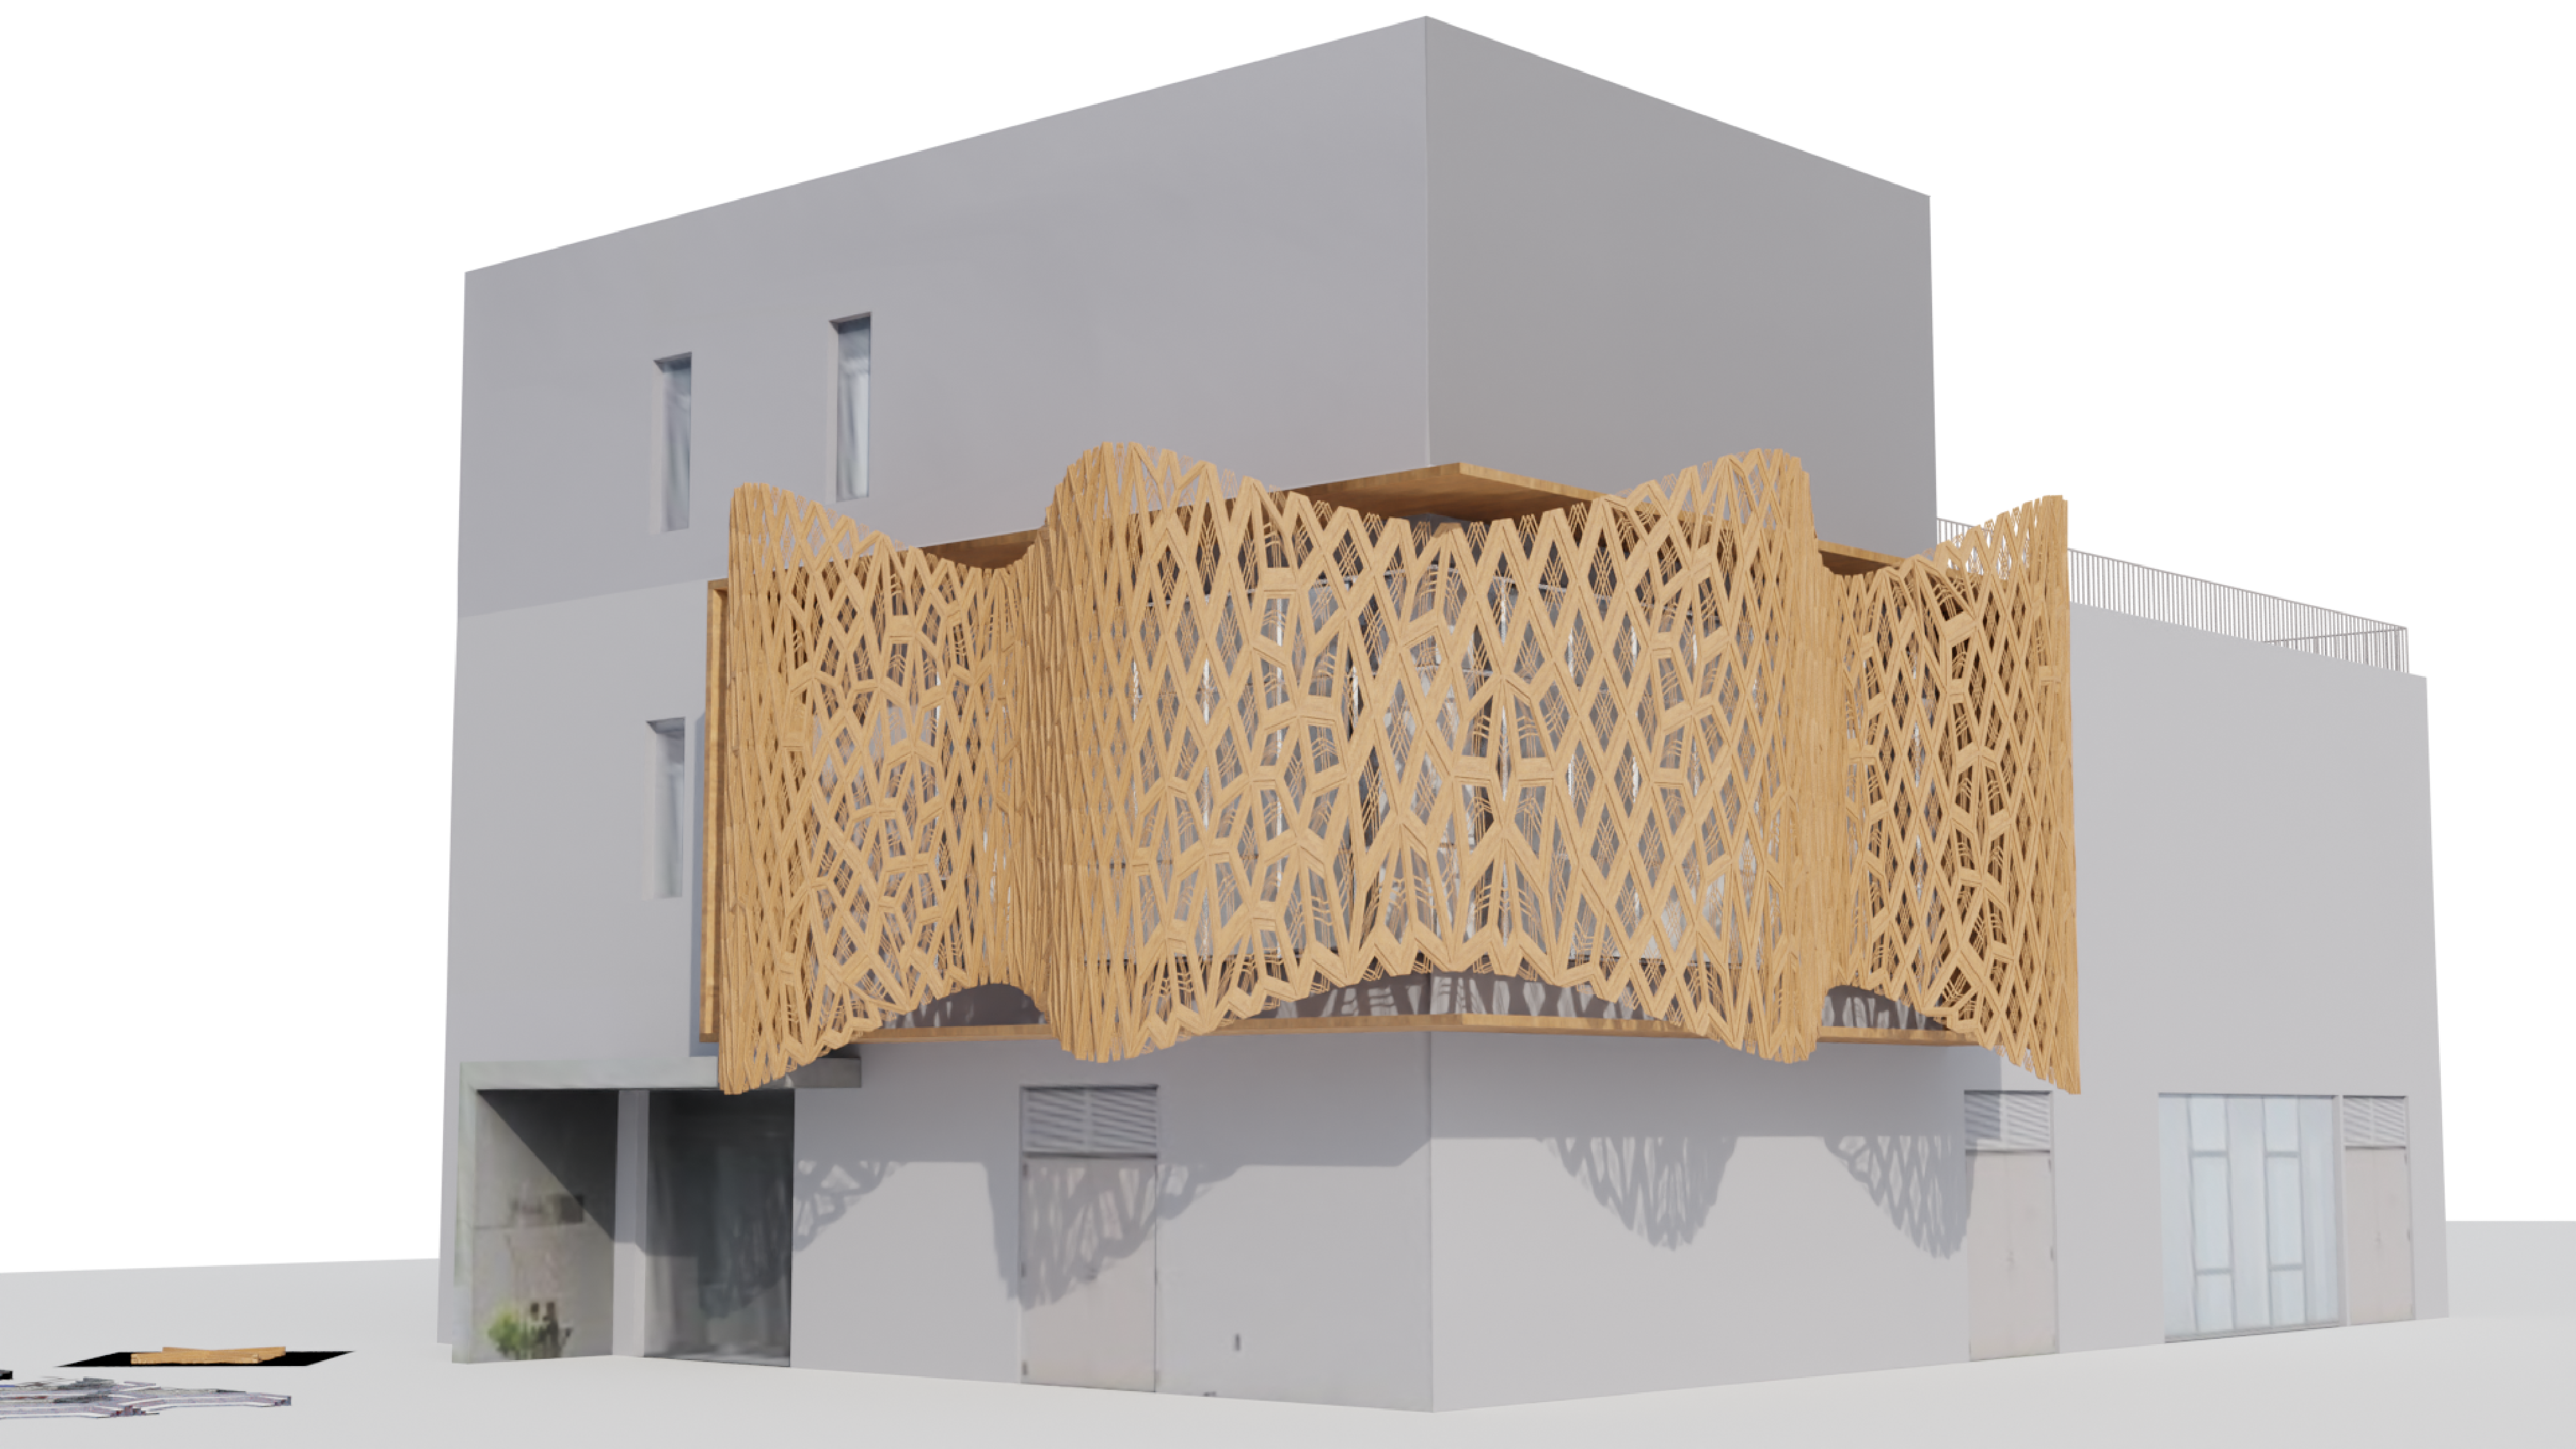
\includegraphics[width=1\linewidth]{Images/Pattern 1/0009}} &
              {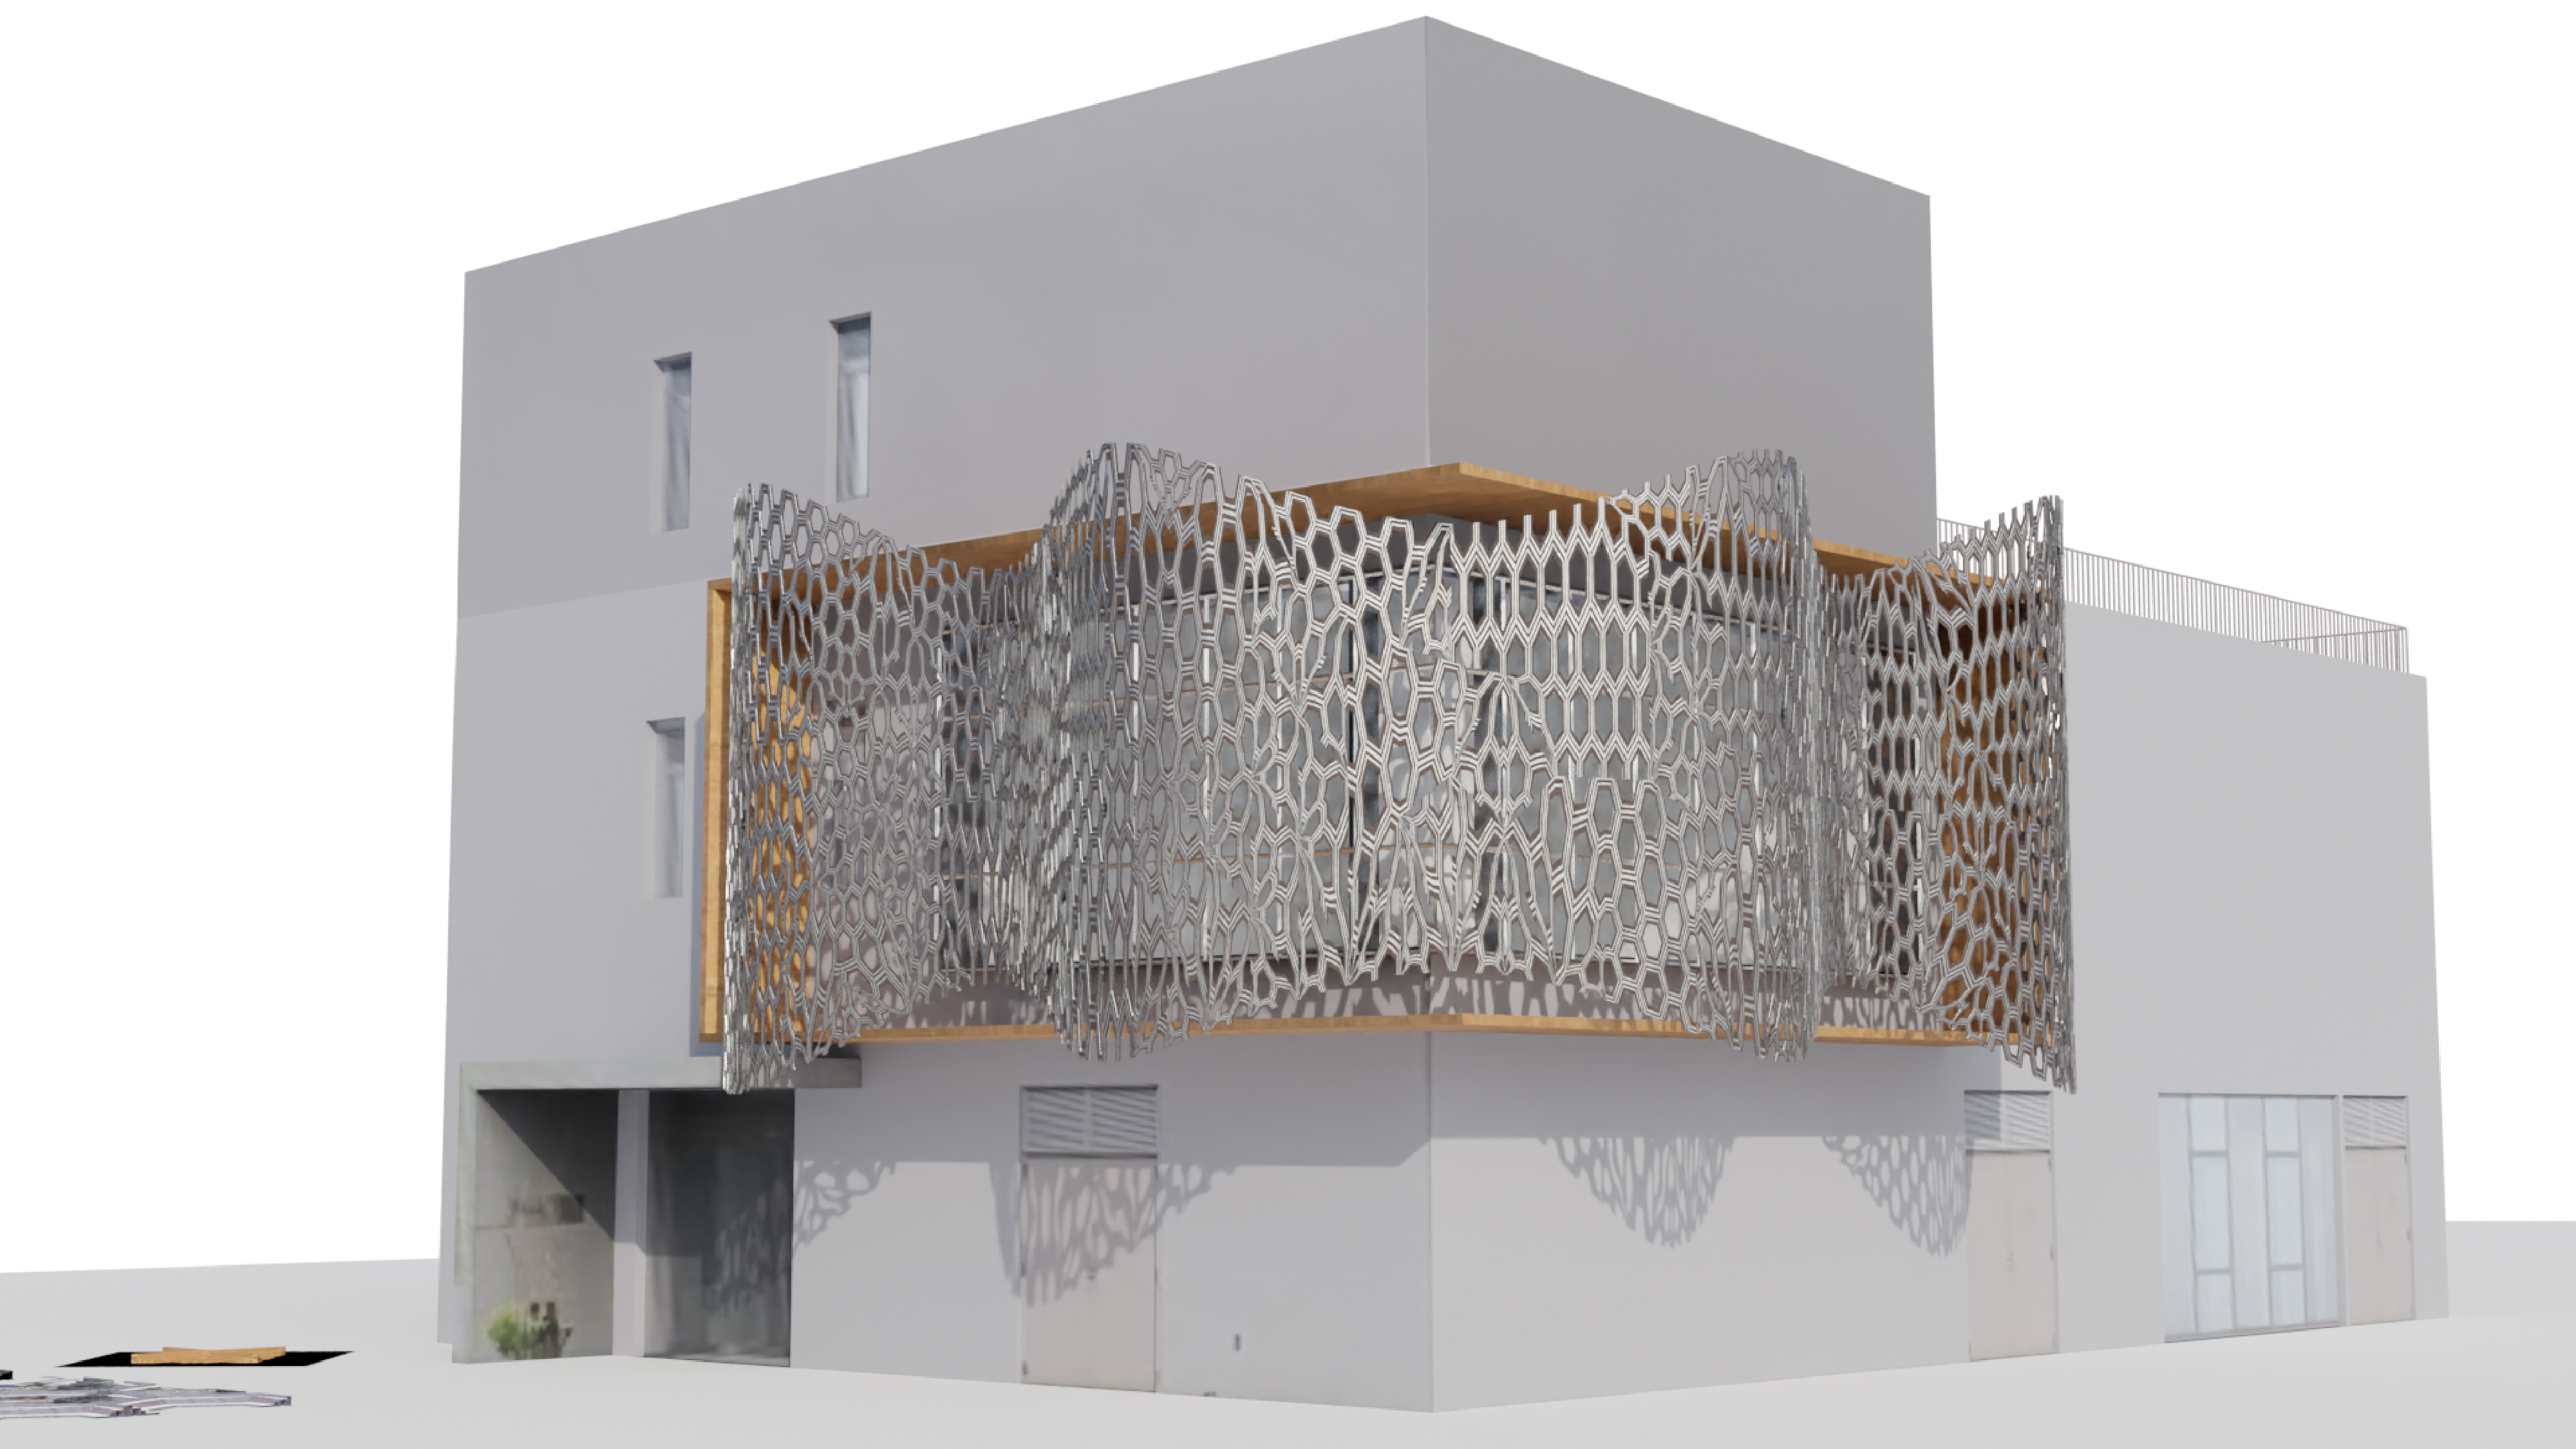
\includegraphics[width=1\linewidth]{Images/Pattern 2/0009}} &
              {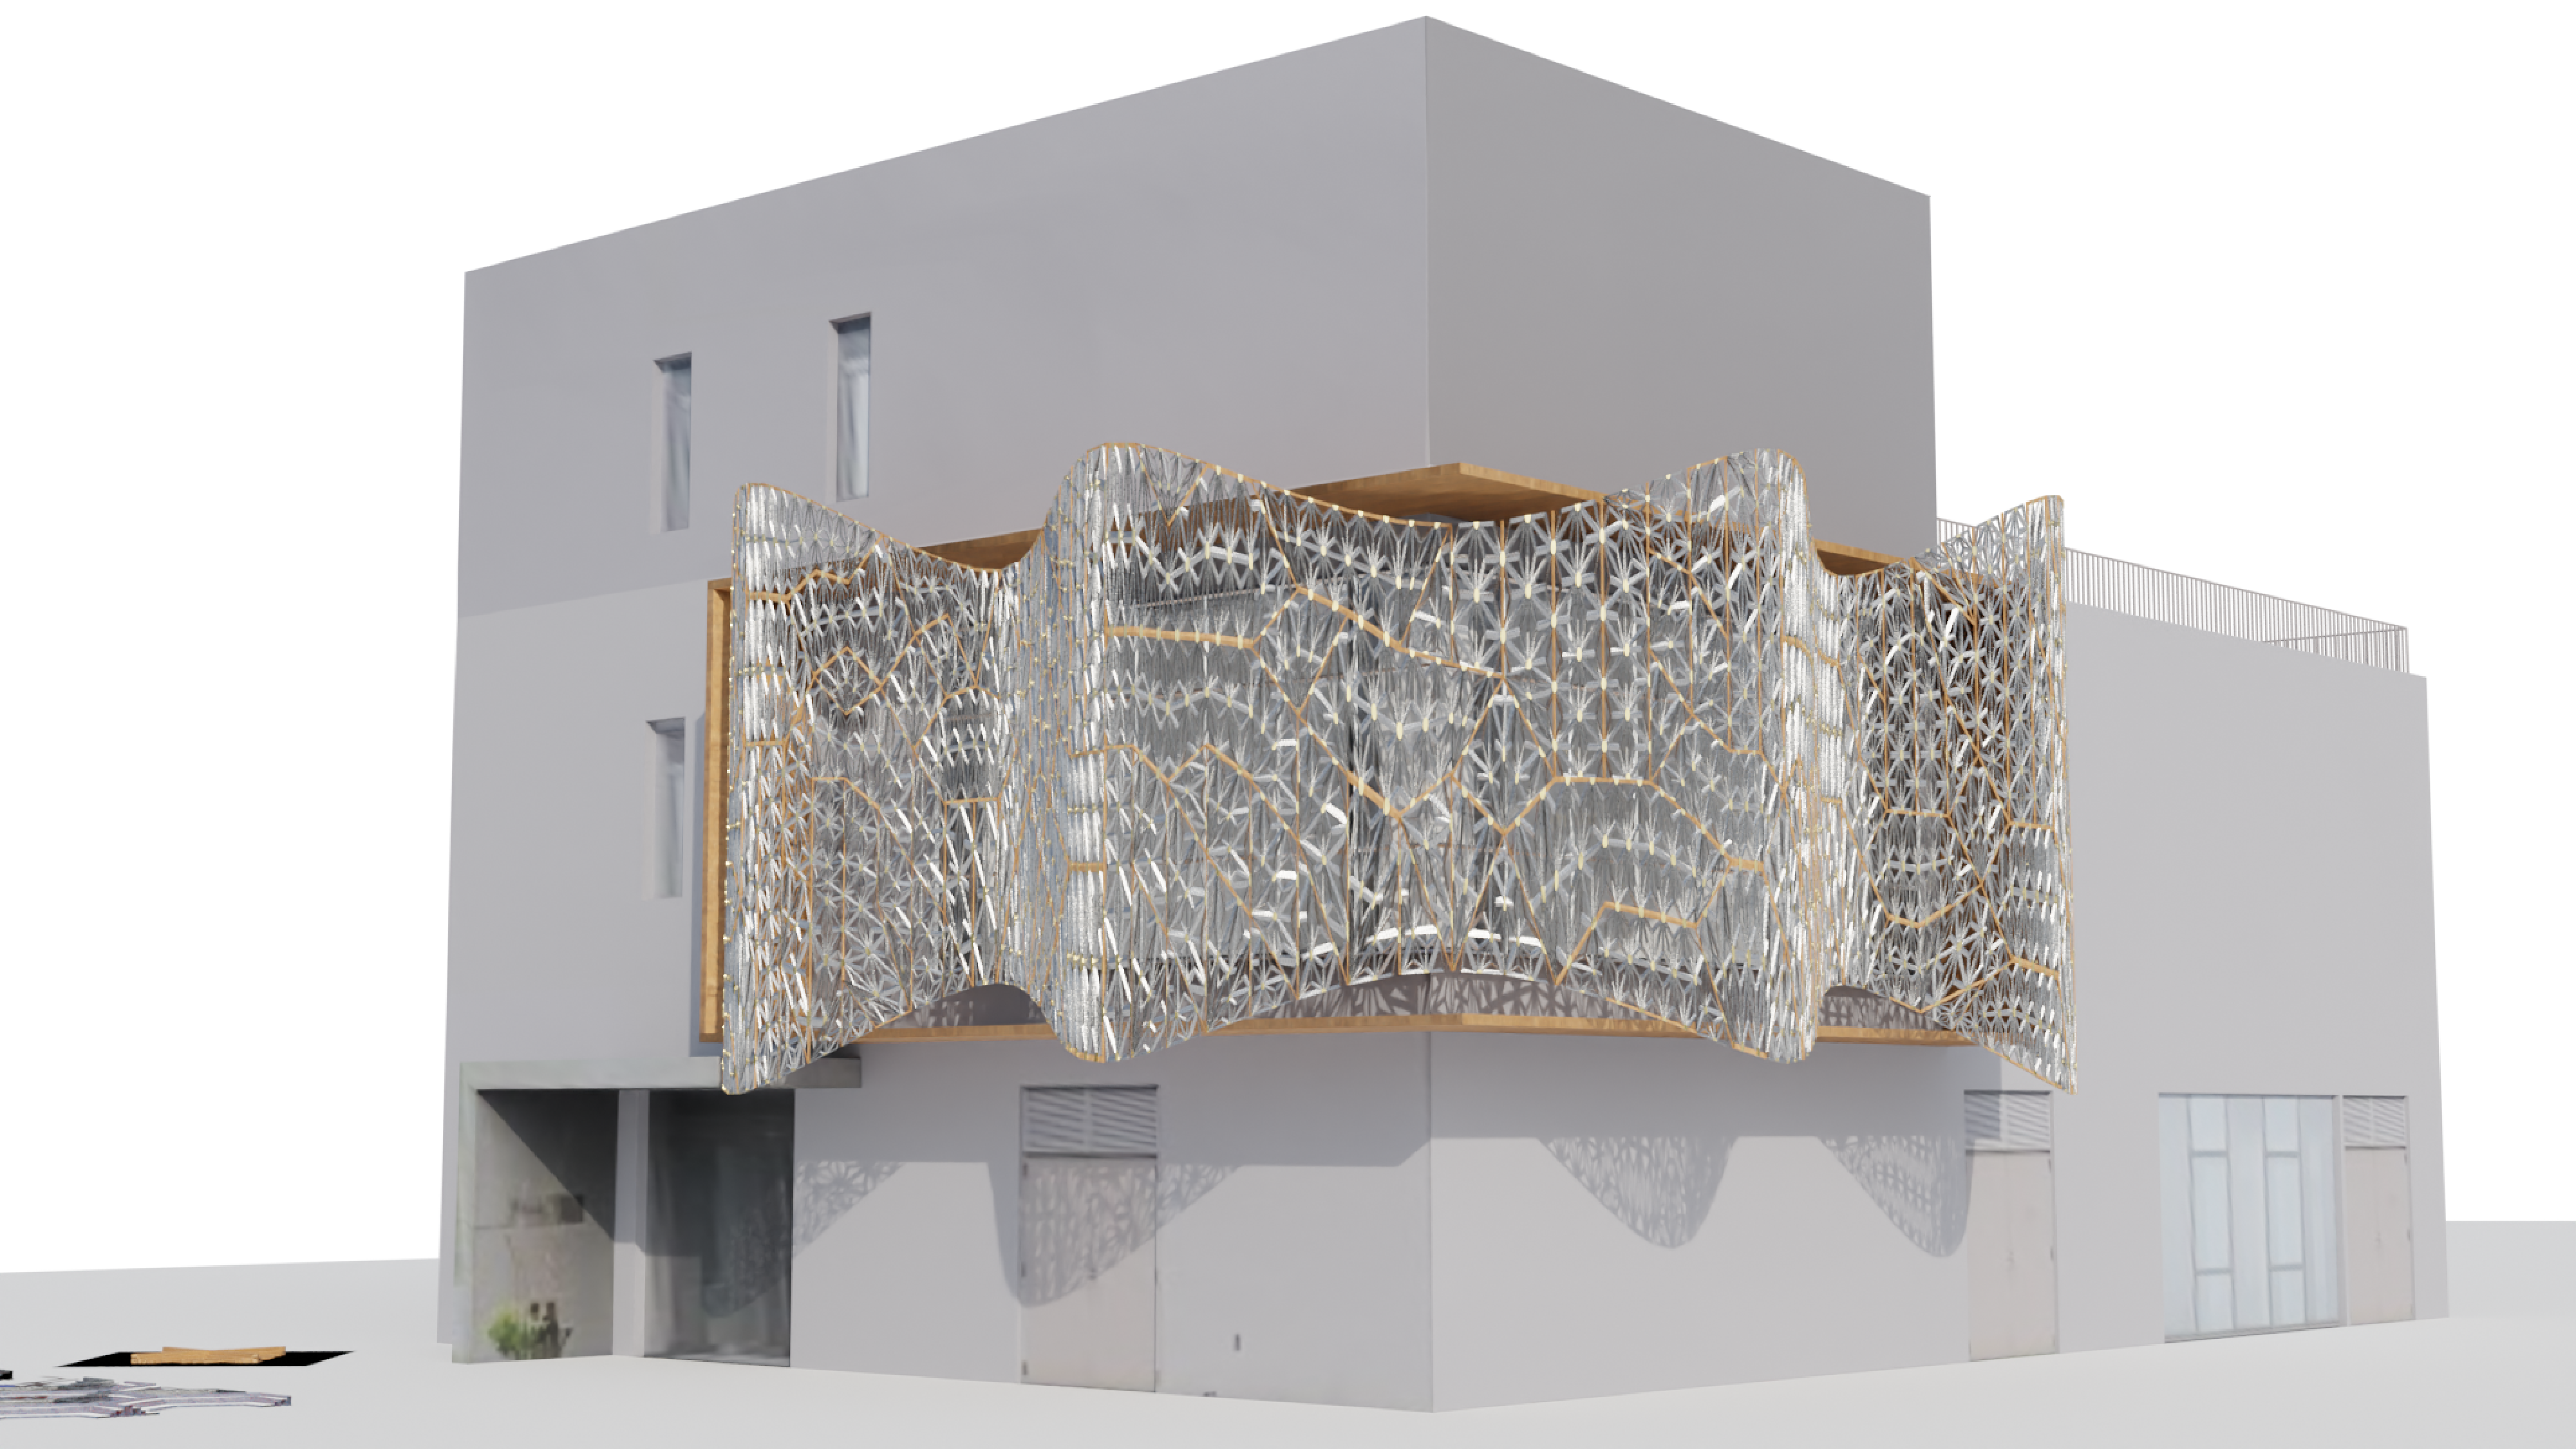
\includegraphics[width=1\linewidth]{Images/Pattern 3/0009}} \\
            \midrule
            \textit{Level 10} &  &  &
            \\
            {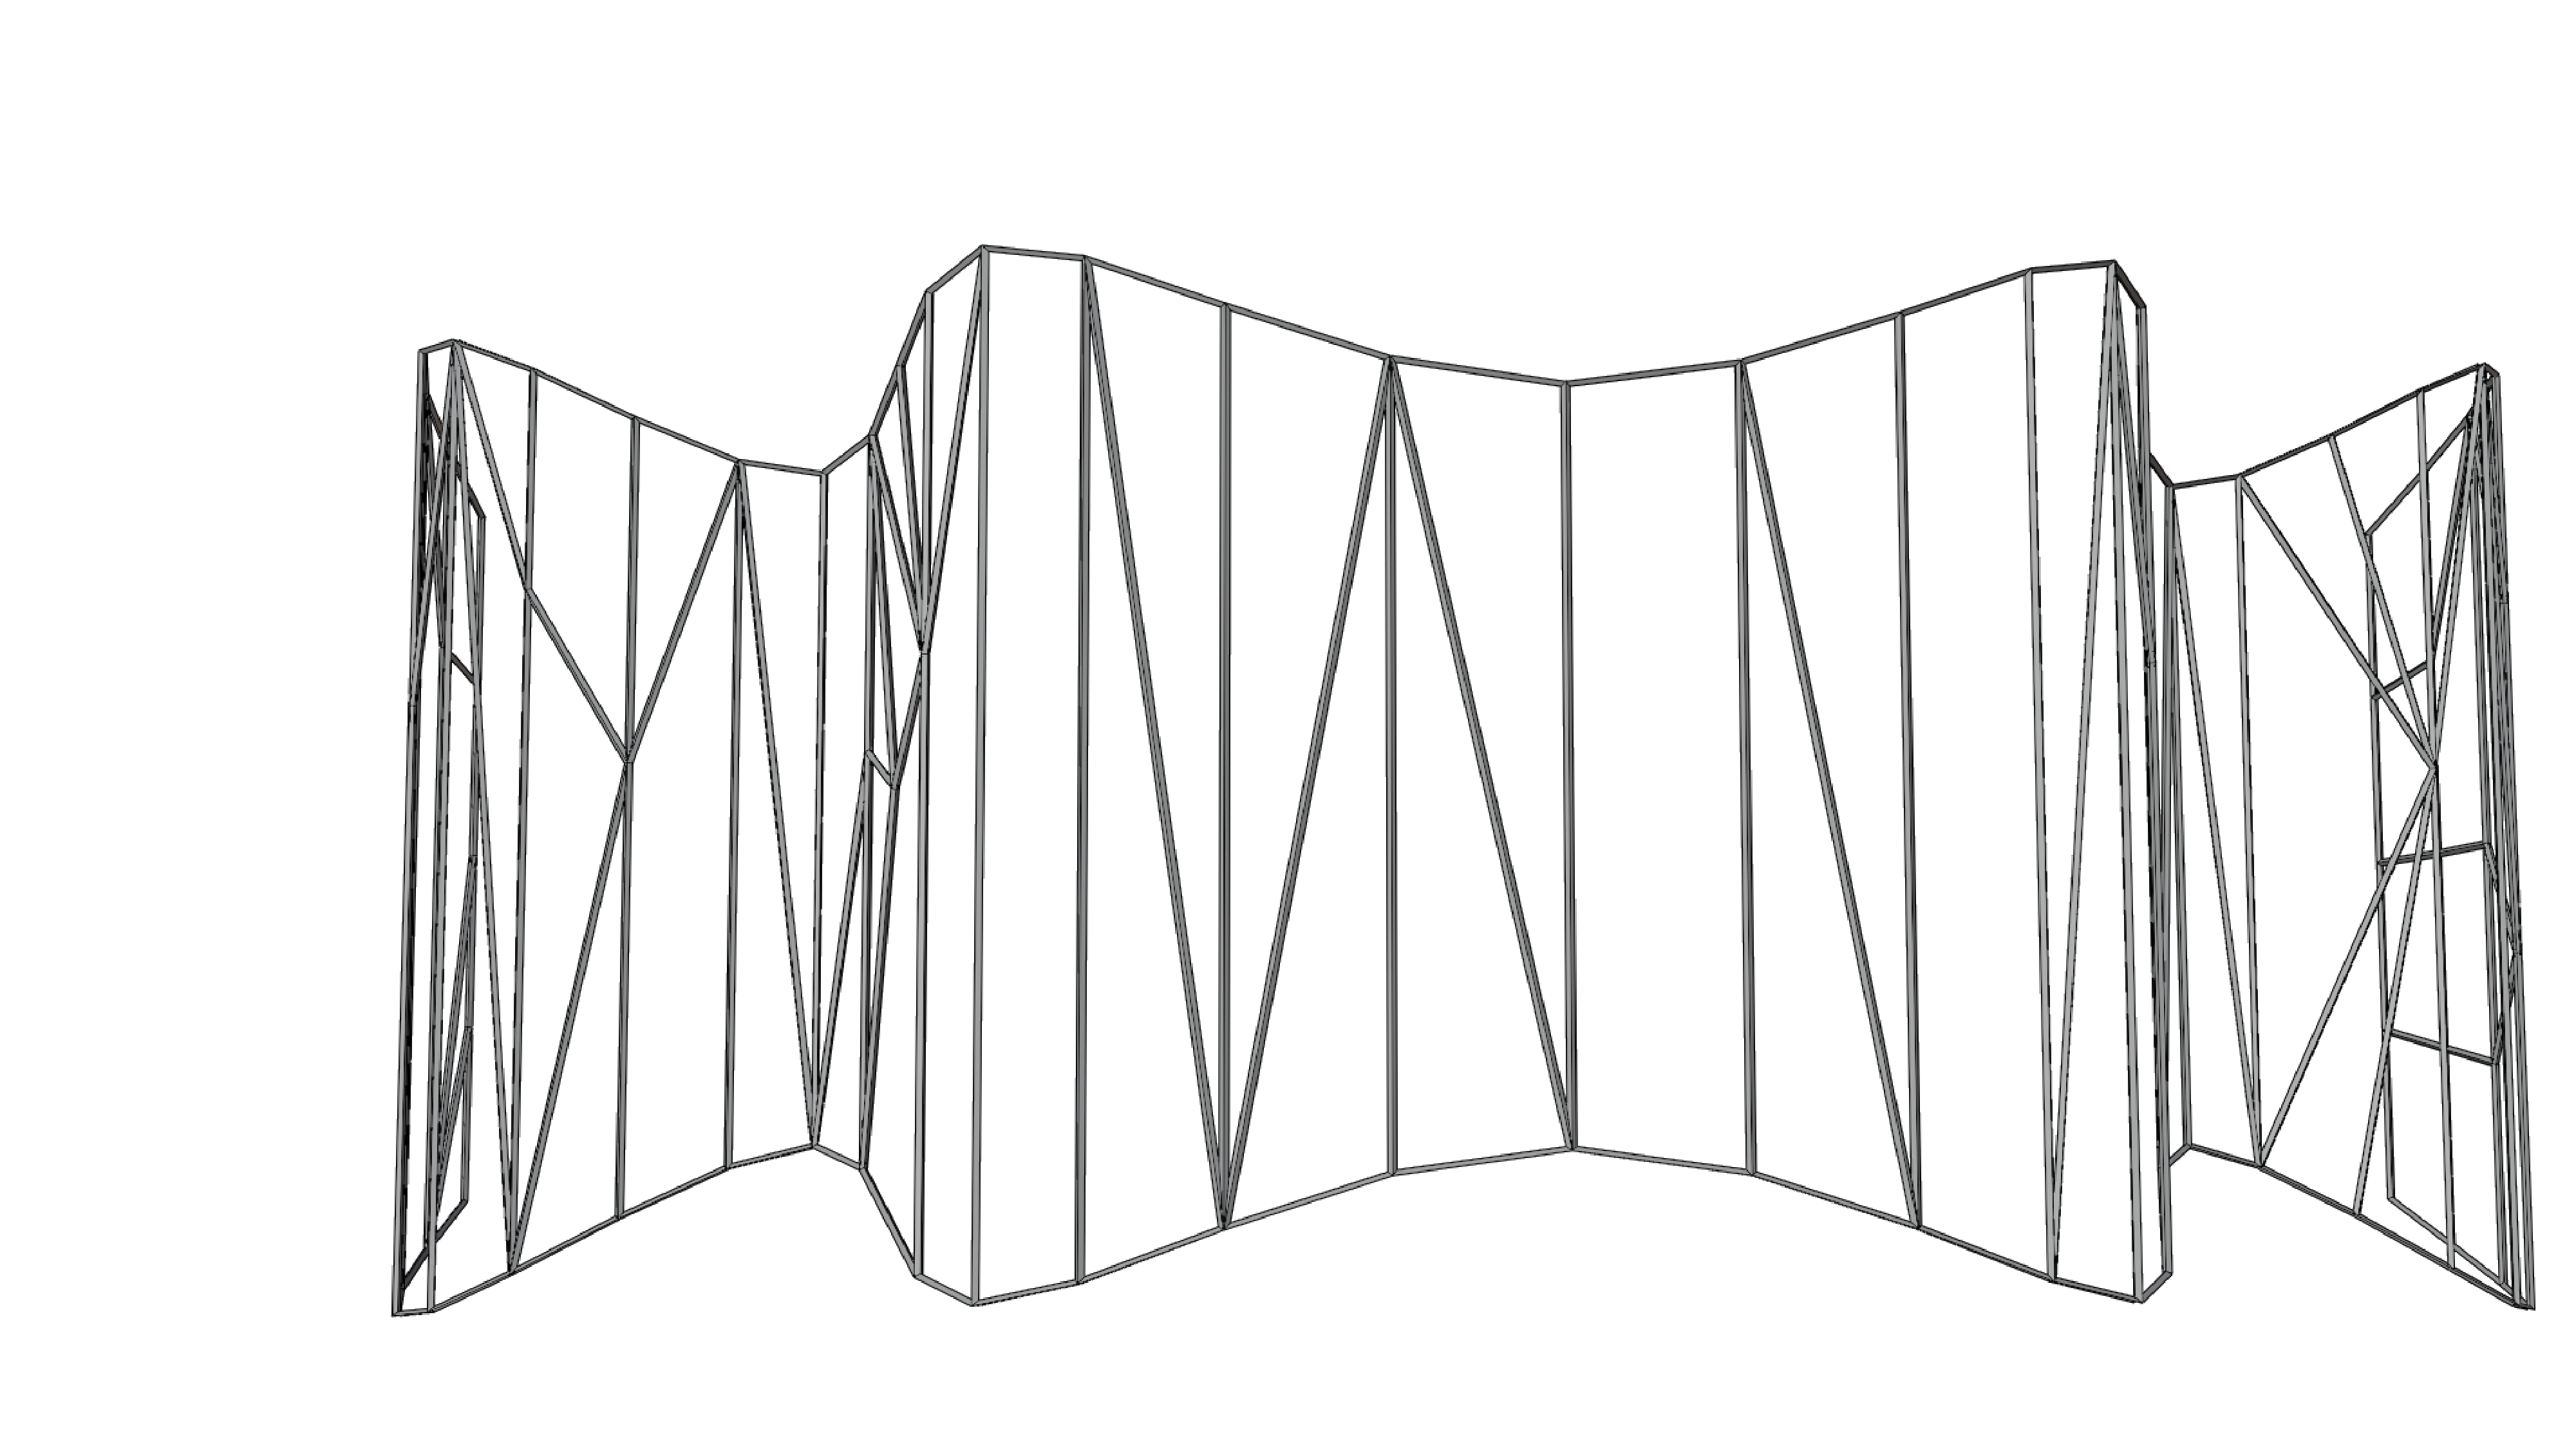
\includegraphics[width=1\linewidth]{Images/Wall 0/0010}} &
              {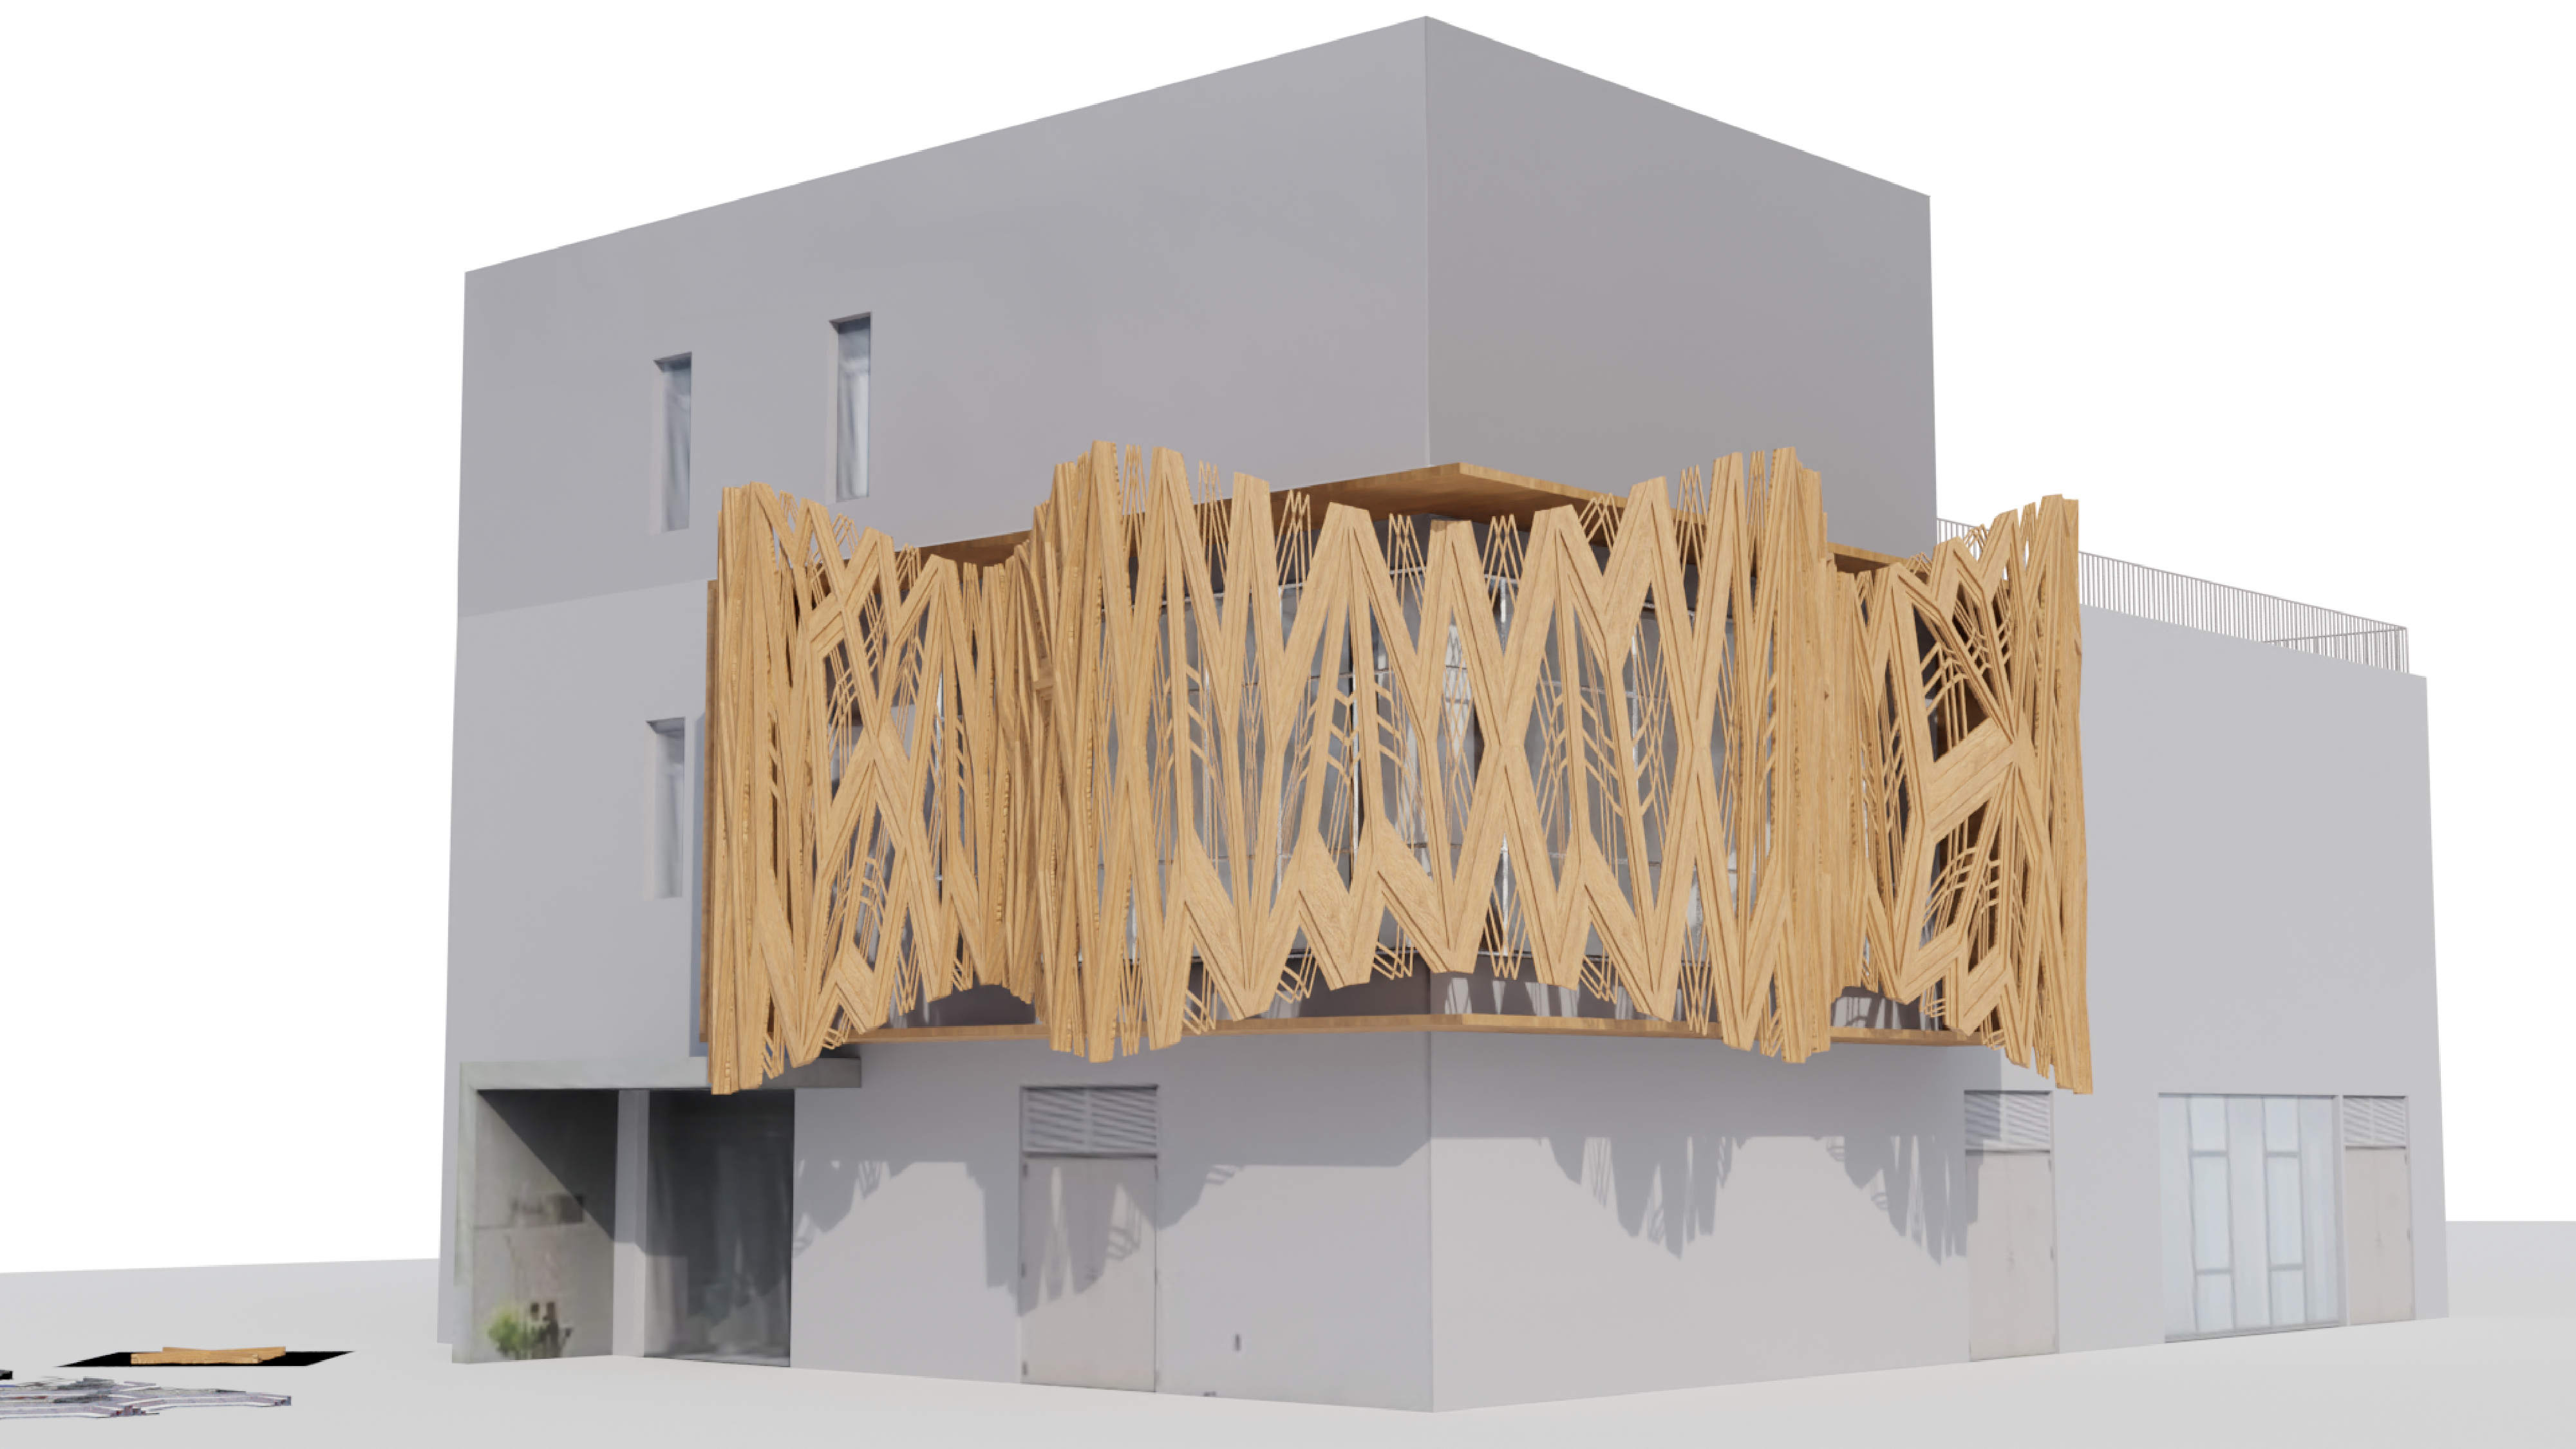
\includegraphics[width=1\linewidth]{Images/Pattern 1/0010}} &
              {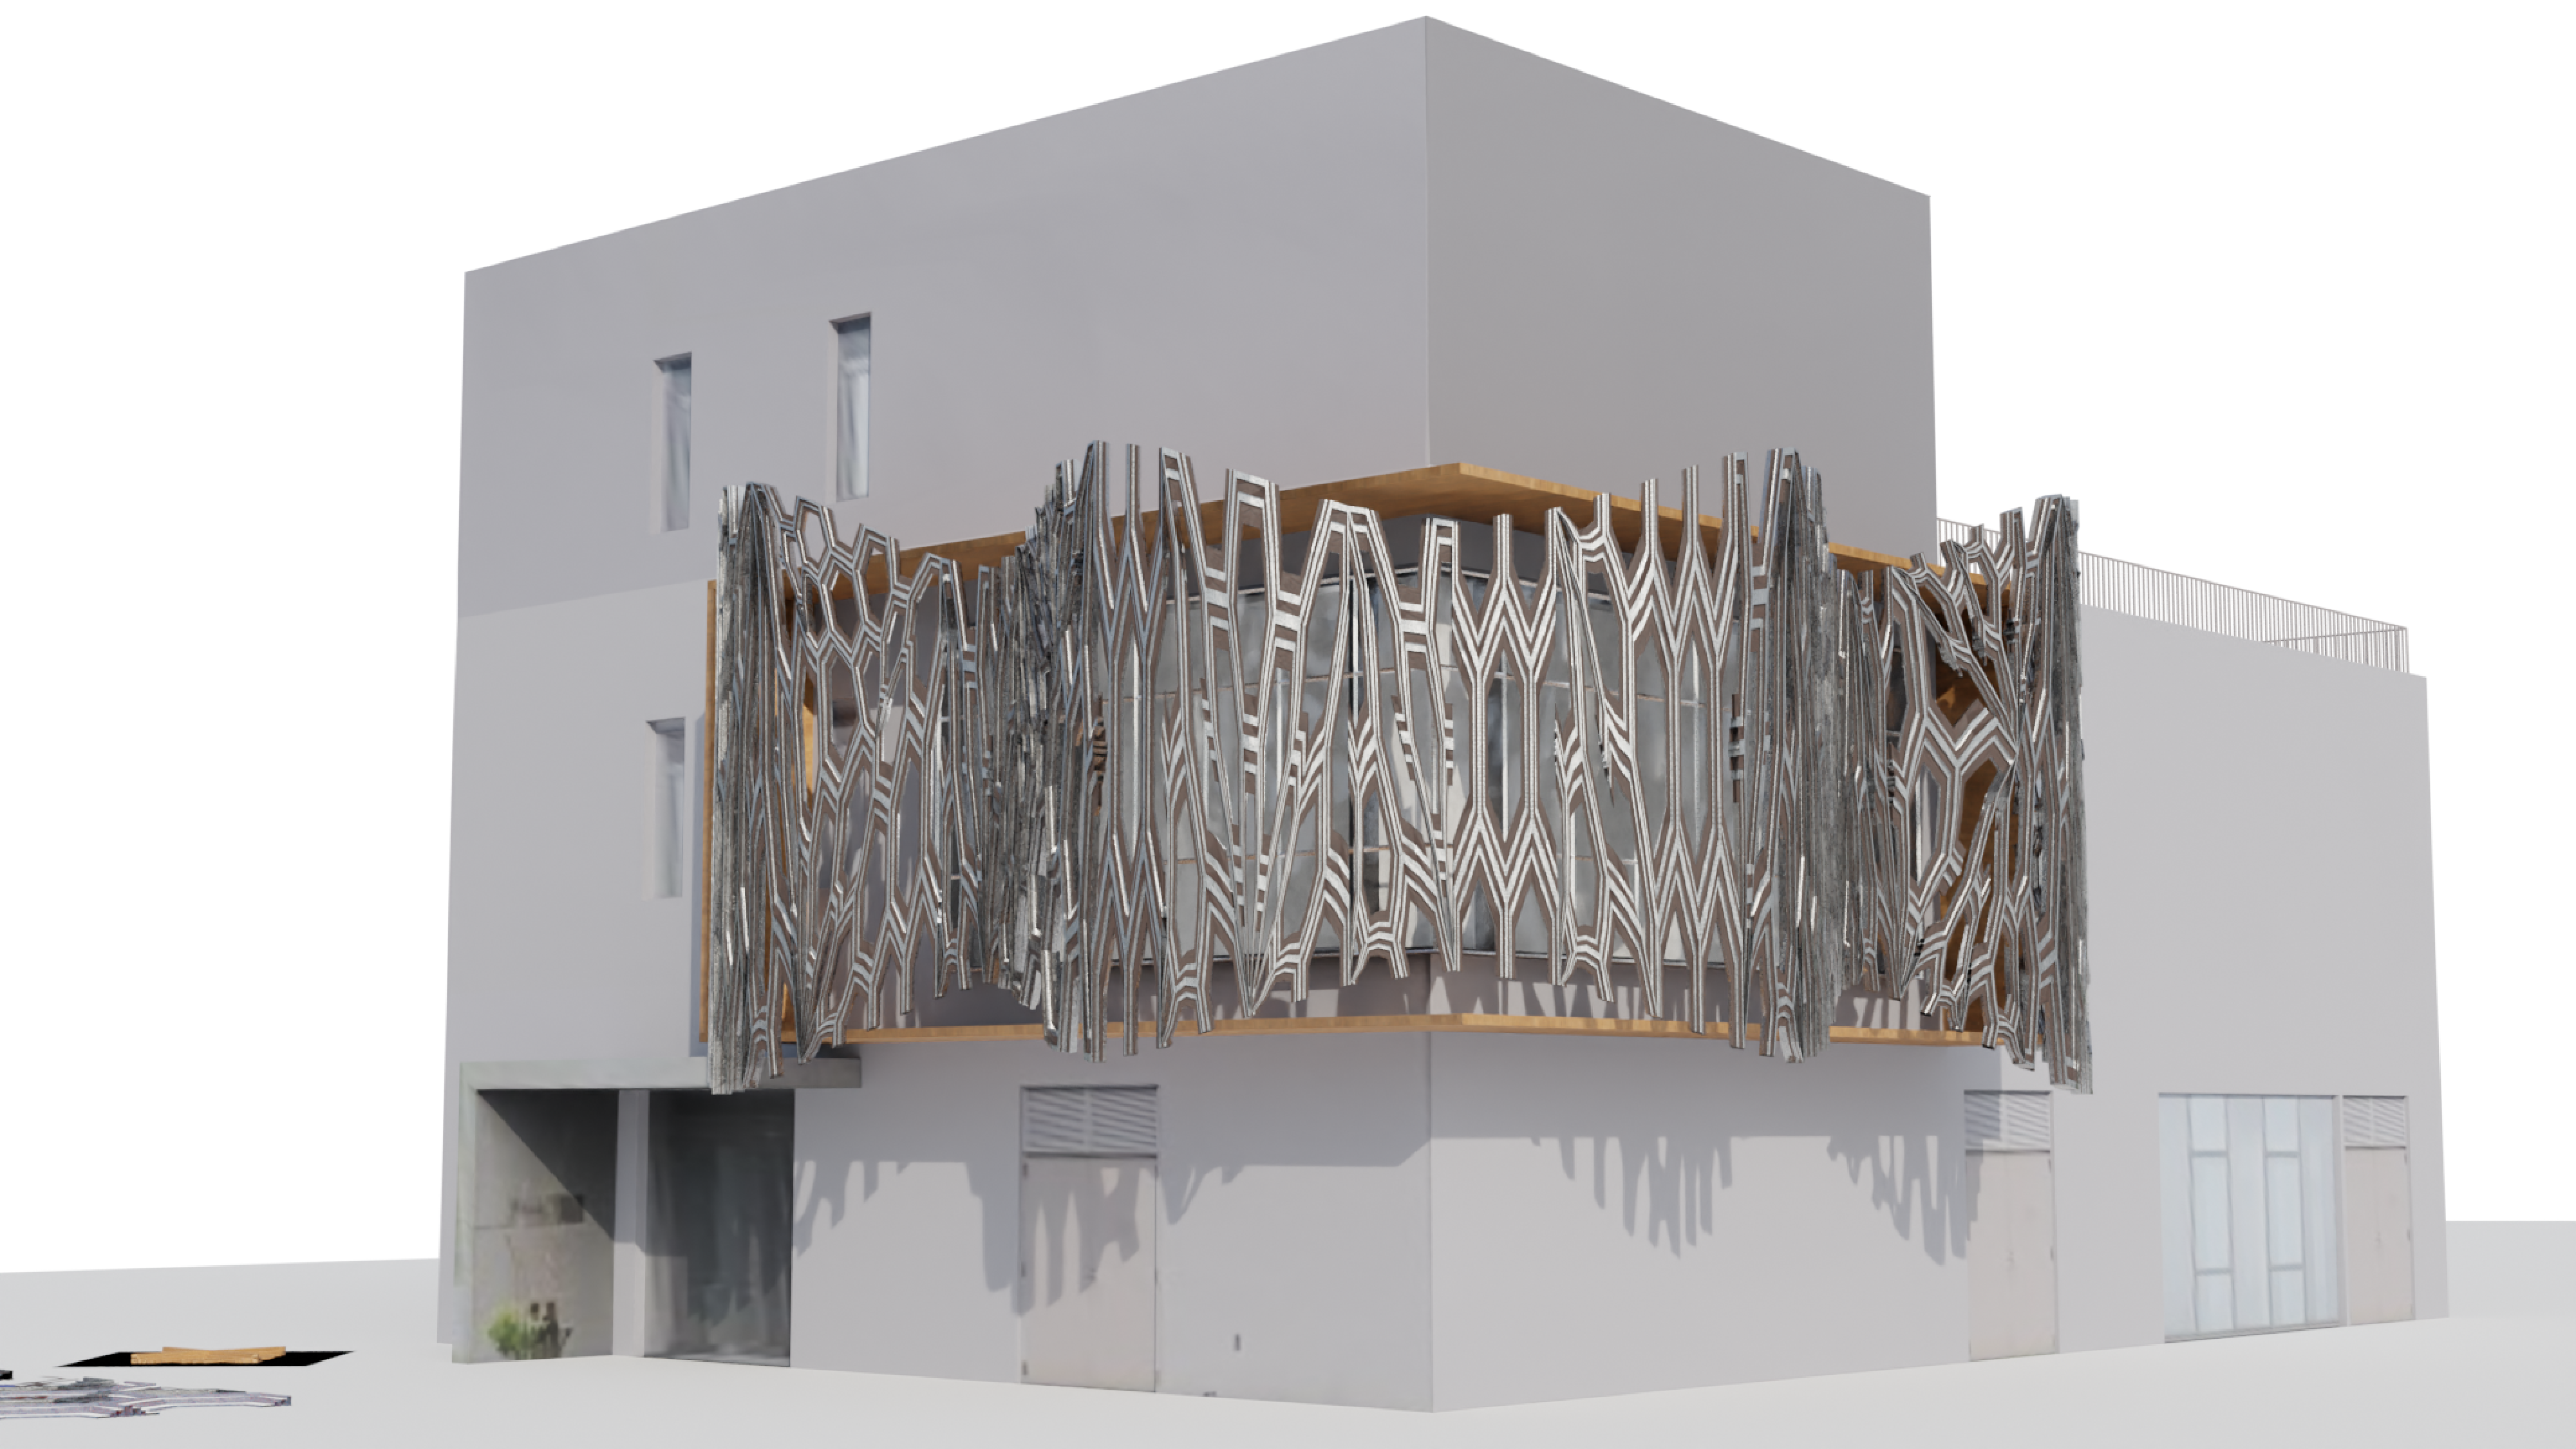
\includegraphics[width=1\linewidth]{Images/Pattern 2/0010}} &
              {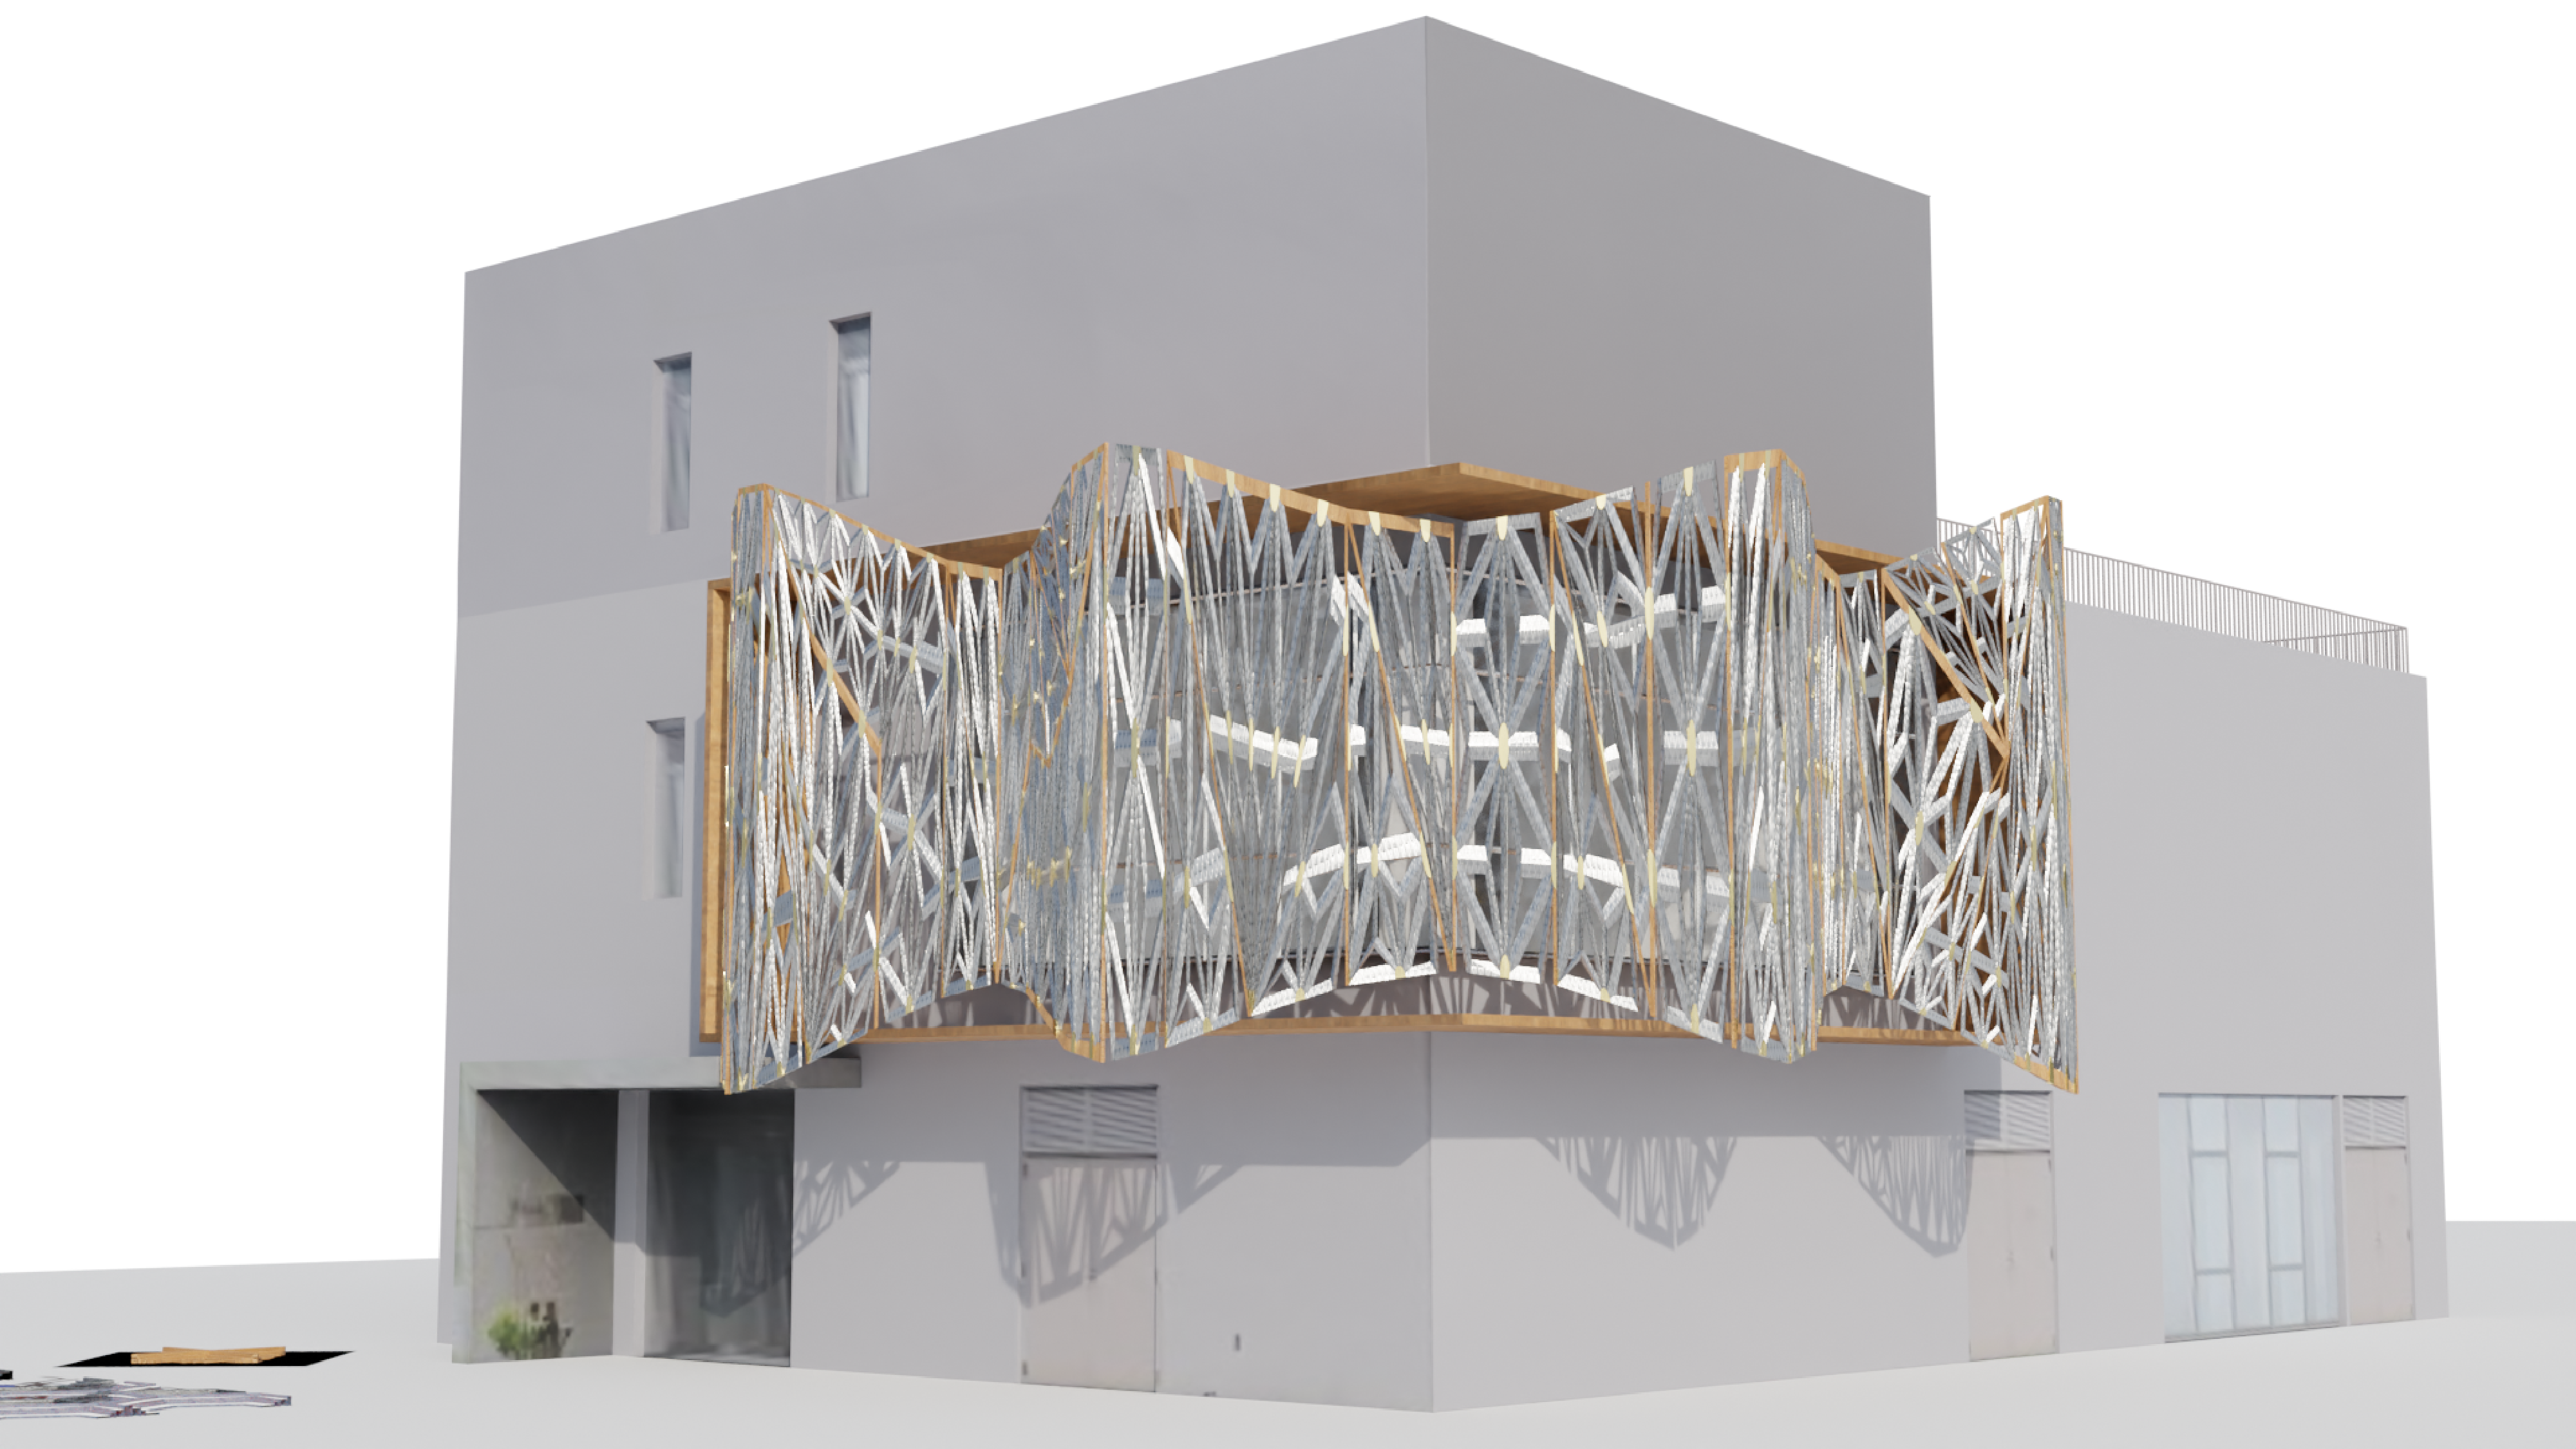
\includegraphics[width=1\linewidth]{Images/Pattern 3/0010}} \\
            \bottomrule
        \end{tabularx}
    \end{table*}



Facade Variations generated for each of the 3 patterns created in Blender and projected during the VR experiment, illustrated in Tables \ref{tab:PatternsVariationsPart1} and \ref{tab:PatternsVariationsPart2}.

    %%Table: Pattern Variations 1 to 5. Part1
    \begin{table*}[htb]
        \centering
        \small
        \caption{Patterns variations for the First five levels of complexity}
        \label{tab:PatternsVariationsPart1}
        \begin{tabularx}
        {\textwidth}{p{3cm} >{\centering\arraybackslash}X >{\centering\arraybackslash}X >{\centering\arraybackslash}X }
            \toprule
            \textit{Description} &
              \textit{Pattern 1} &
              \textit{Pattern 2} &
              \textit{Pattern 3} \\
            \midrule
            \text{Pattern Name} & Hishi Pattern & Tortoise shells & Asanoha Pattern\\

            \midrule
            \textit{Base Module} &  &  &
            \\
            {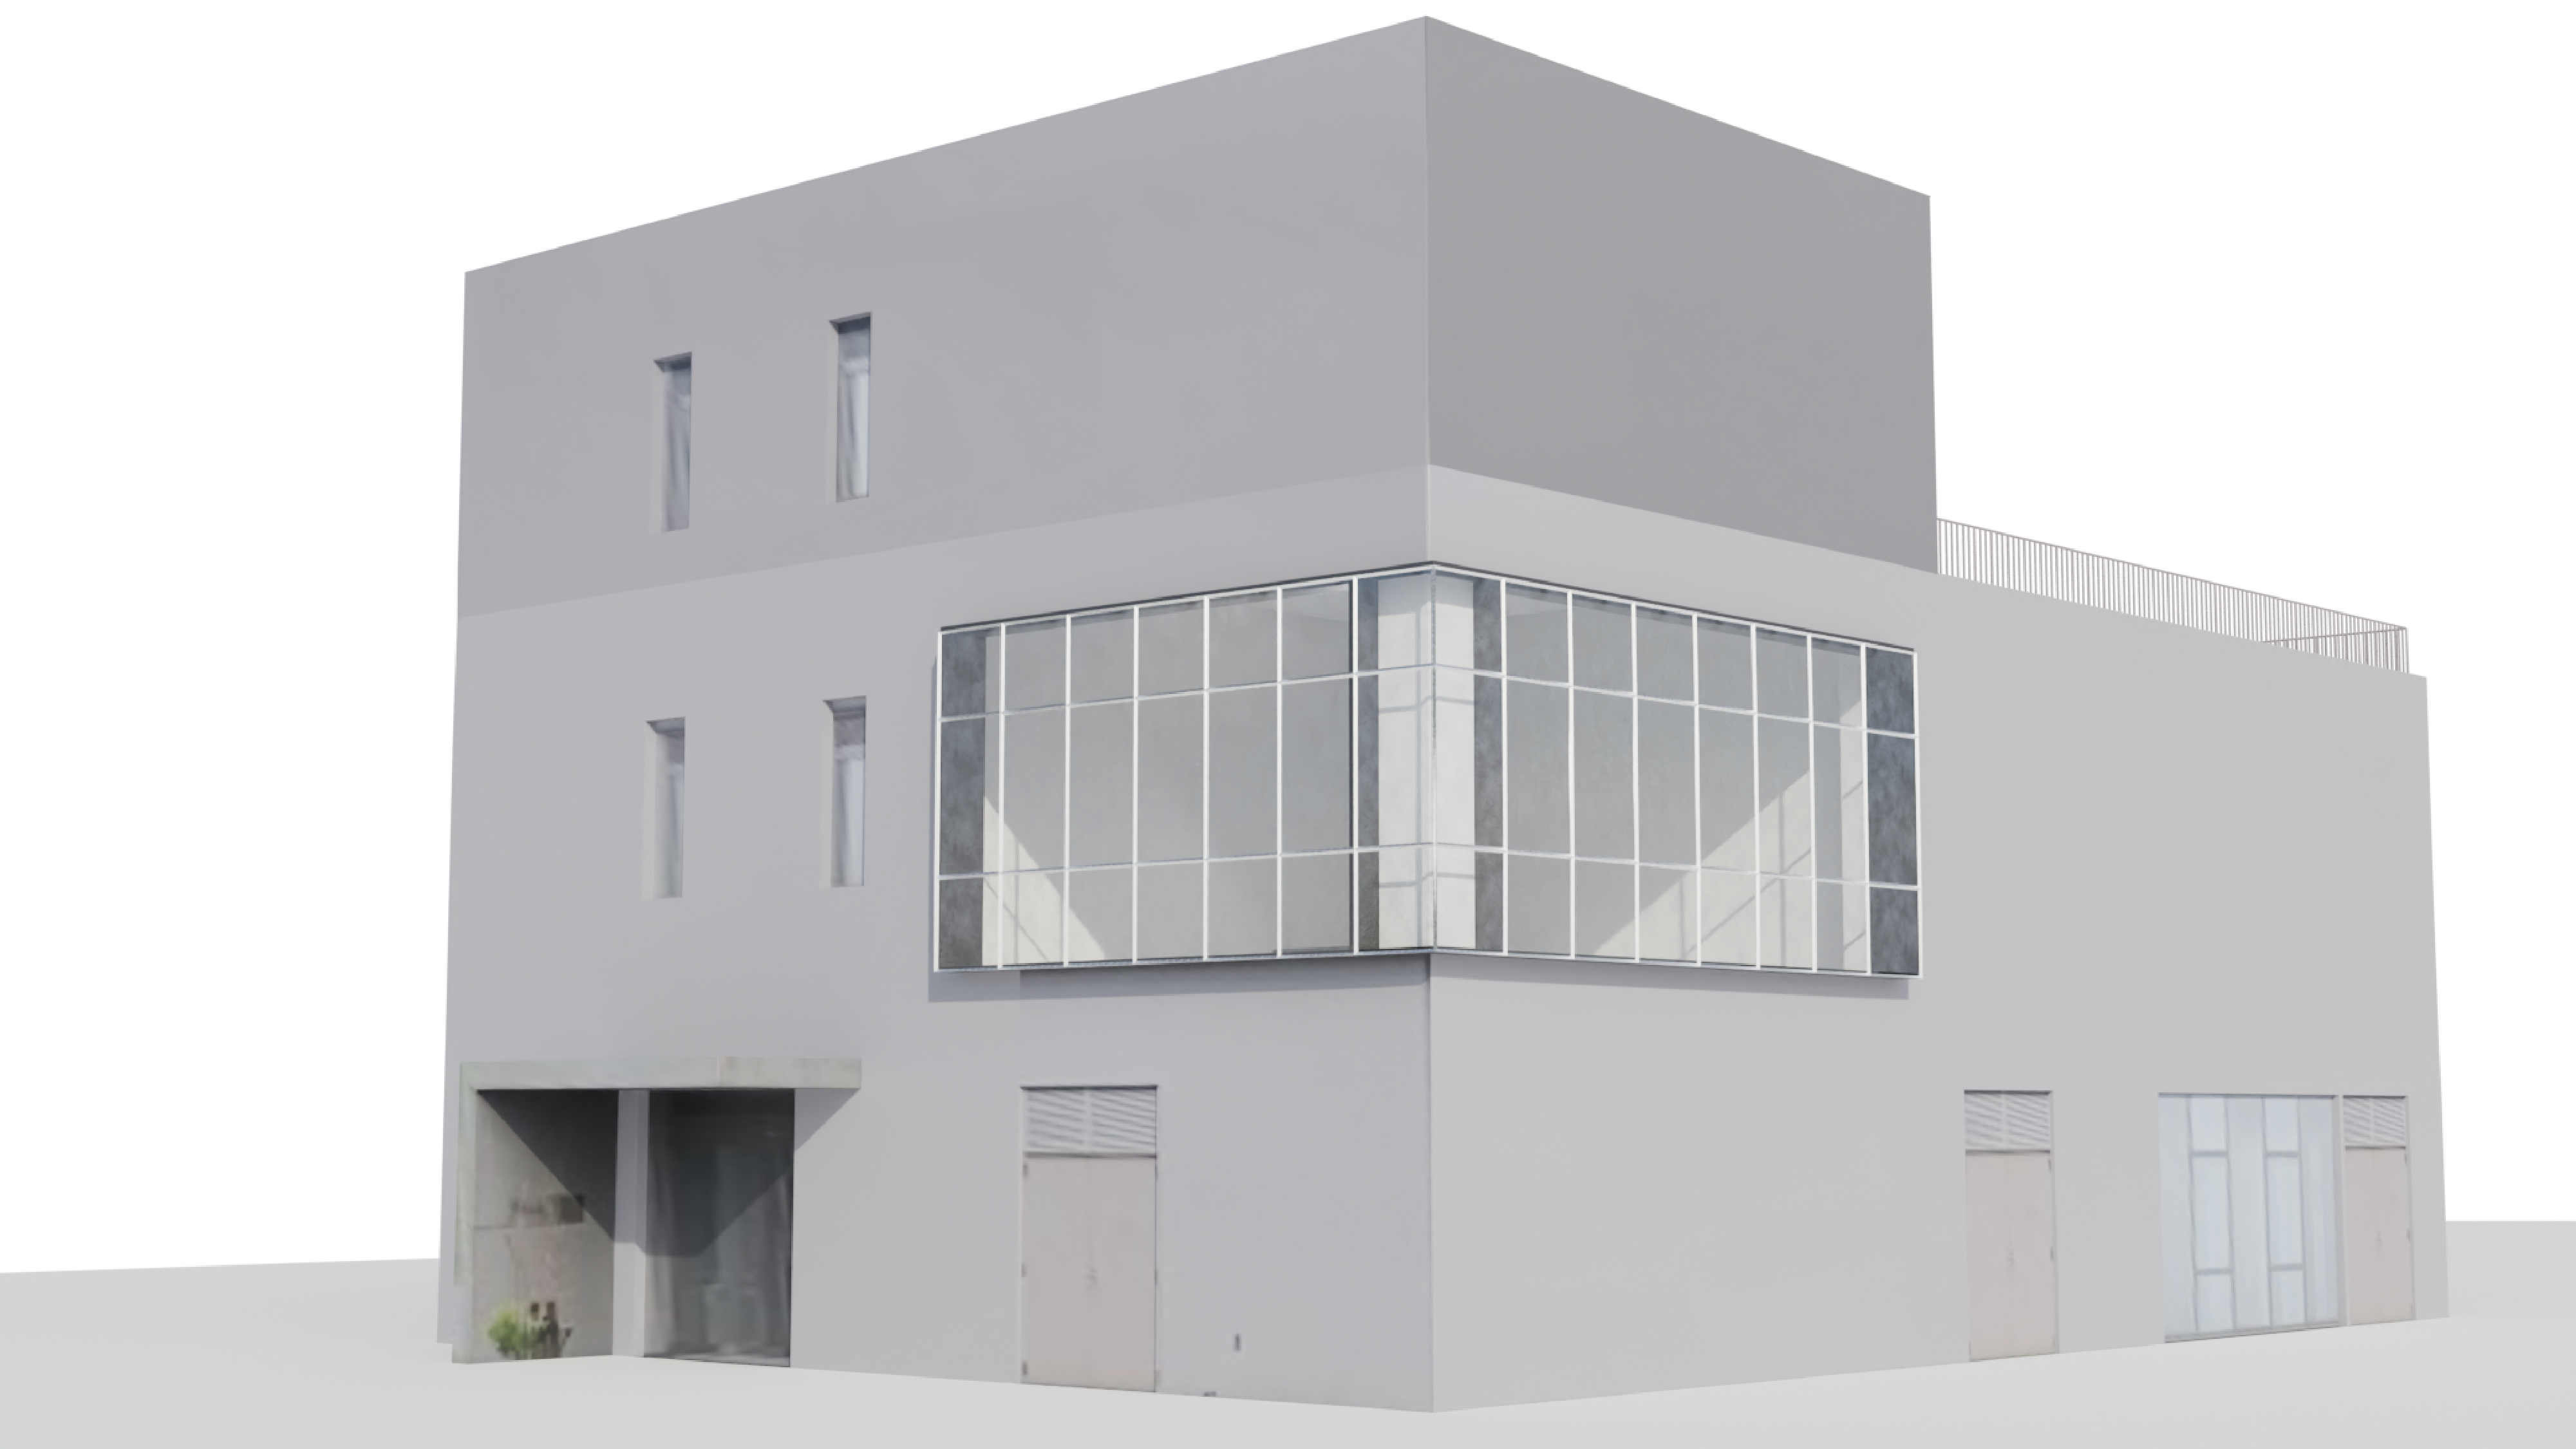
\includegraphics[width=1\linewidth]{Images/Base Module/Building}} &
              {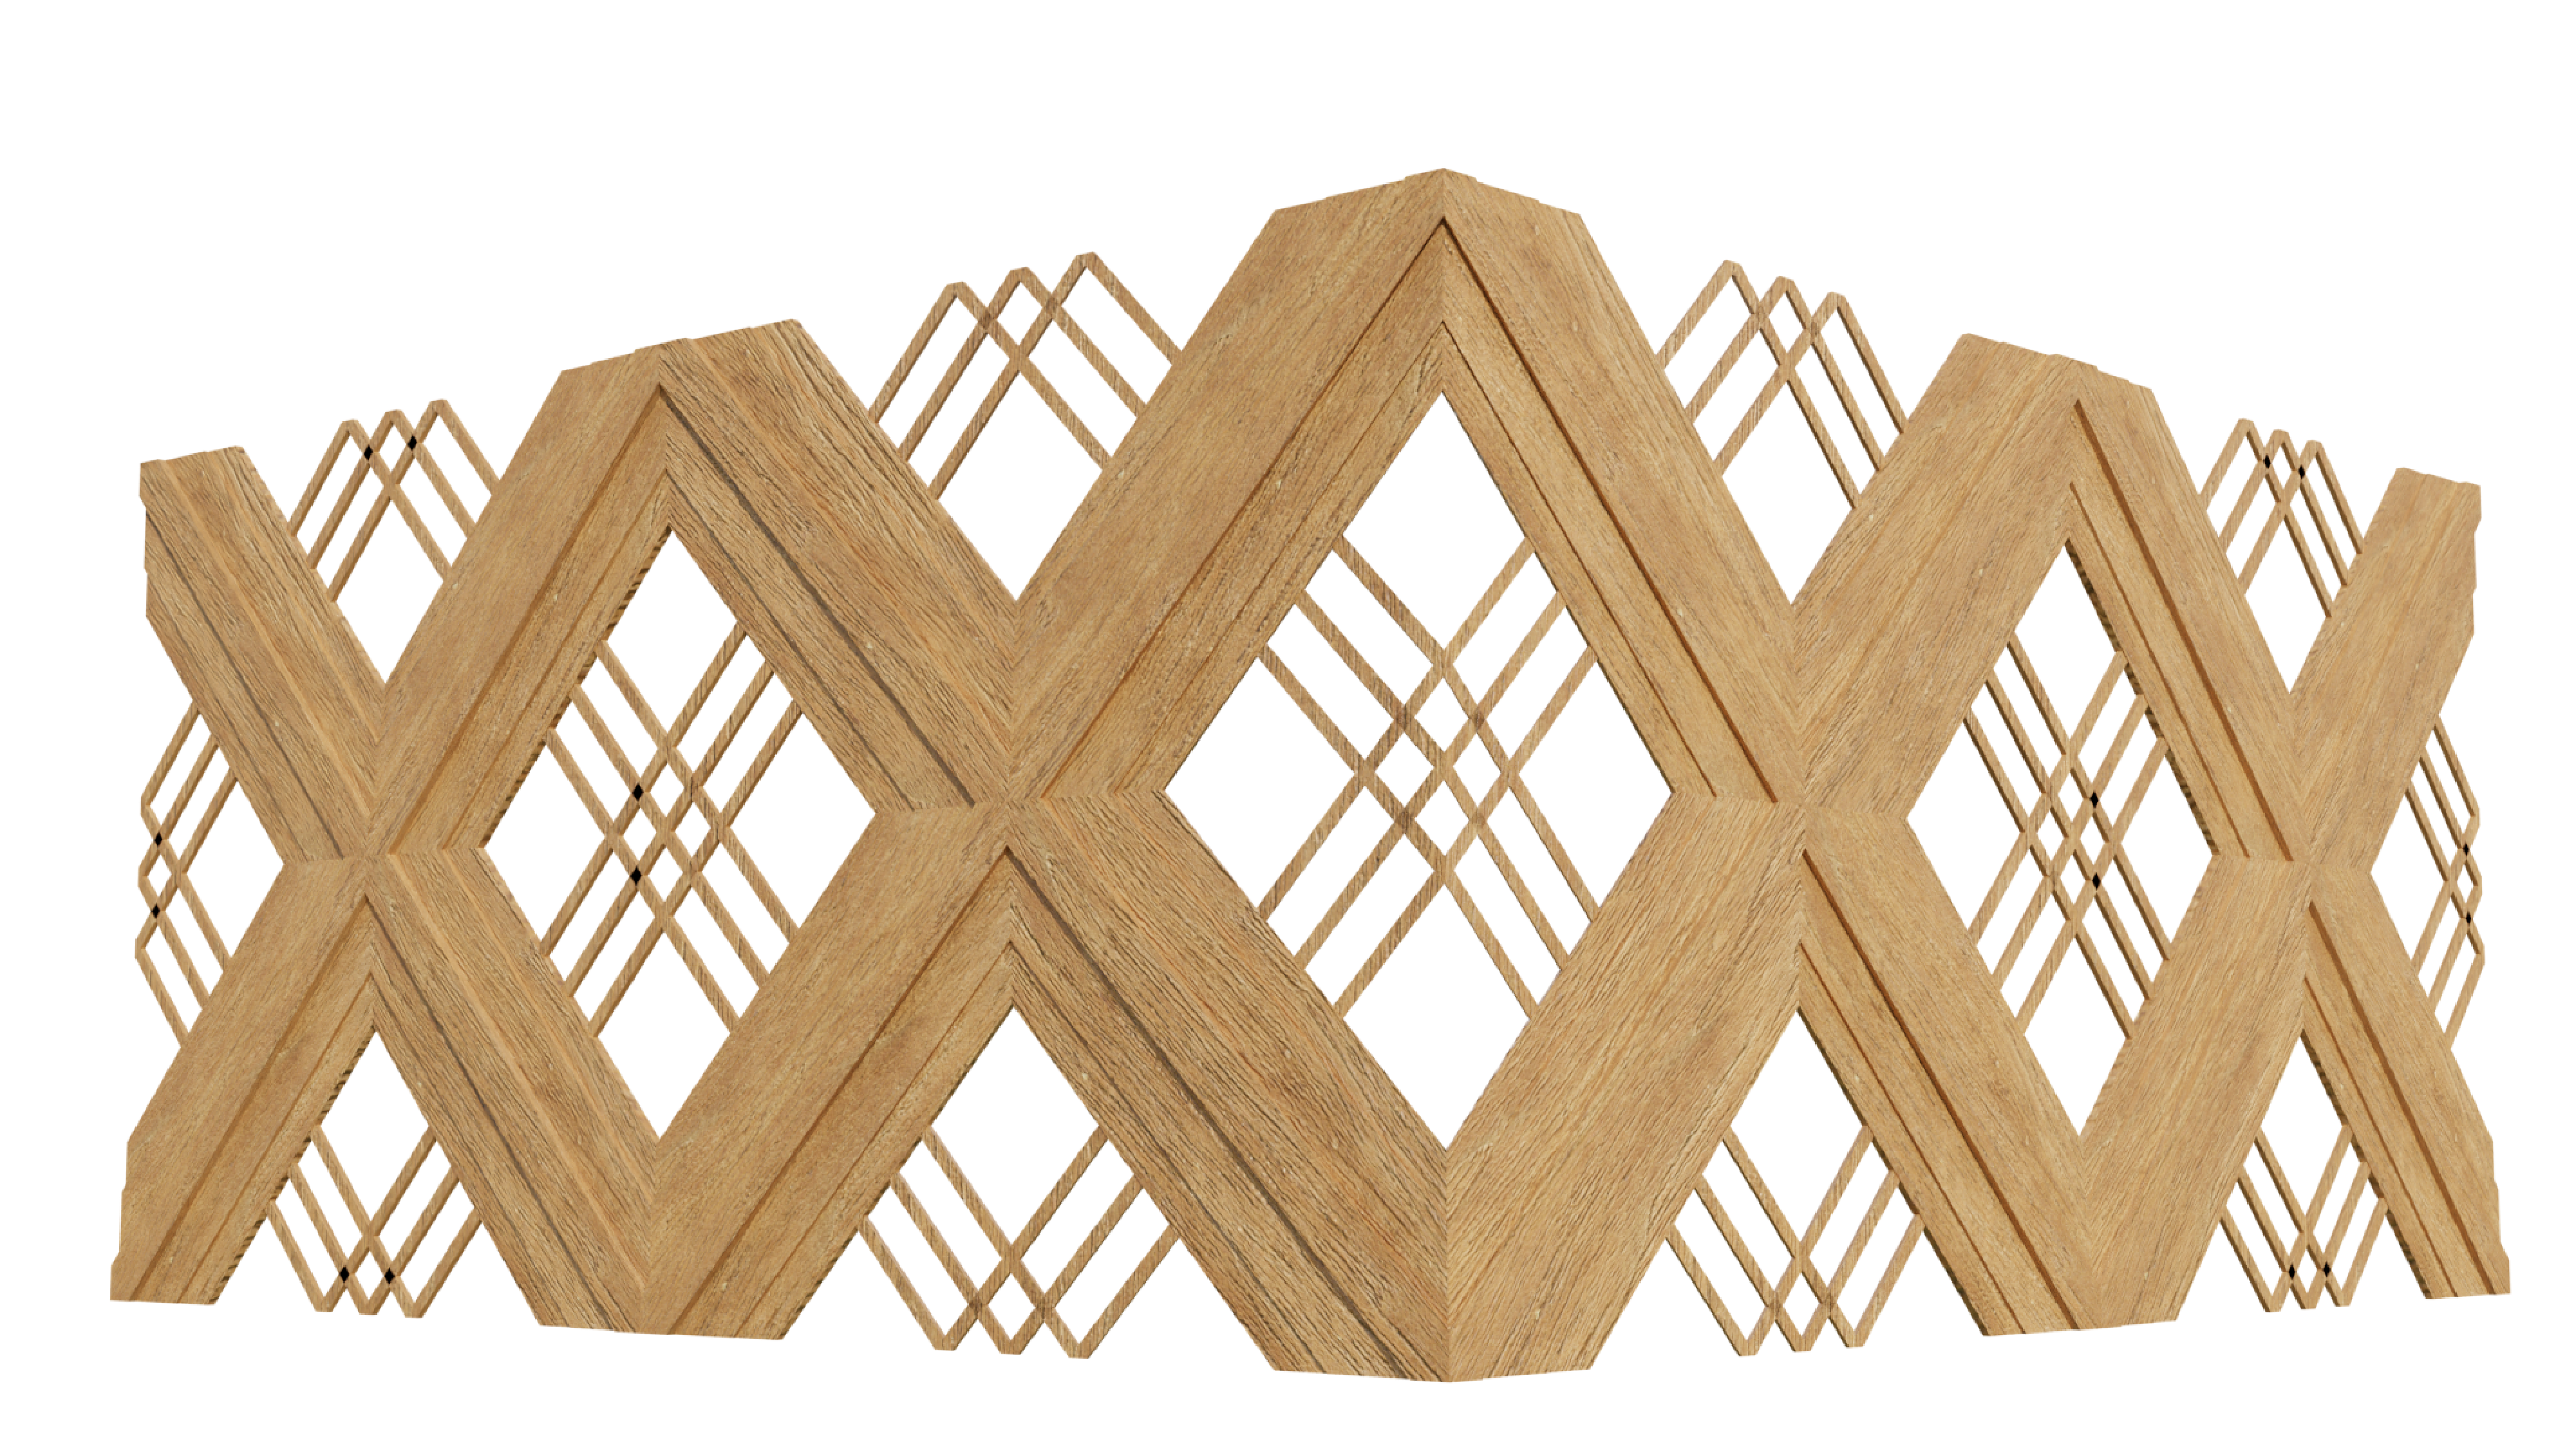
\includegraphics[width=1\linewidth]{Images/Base Module/Pattern1}} &
              {\includegraphics[width=1\linewidth]{Images/Base Module/Pattern2}} &
              {\includegraphics[width=1\linewidth]{Images/Base Module/Pattern3}} \\
            \midrule

            \textit{Mesh complexity Level} &
              \textit{Pattern 1} &
              \textit{Pattern 2} &
              \textit{Pattern 3}\\

            \midrule
            \textit{Level 1} &  &  &
            \\
            {\includegraphics[width=1\linewidth]{Images/Wall 0/0001}} &
                {\includegraphics[width=1\linewidth]{Images/Pattern 1/0001}} &
              {\includegraphics[width=1\linewidth]{Images/Pattern 2/0001}} &
              {\includegraphics[width=1\linewidth]{Images/Pattern 3/0001}} \\
            \midrule
            \textit{Level 2} &  &  &
            \\
            {\includegraphics[width=1\linewidth]{Images/Wall 0/0002}} &
              {\includegraphics[width=1\linewidth]{Images/Pattern 1/0002}} &
              {\includegraphics[width=1\linewidth]{Images/Pattern 2/0002}} &
              {\includegraphics[width=1\linewidth]{Images/Pattern 3/0002}} \\
            \midrule
            \textit{Level 3} &  &  &
            \\
            {\includegraphics[width=1\linewidth]{Images/Wall 0/0003}} &
              {\includegraphics[width=1\linewidth]{Images/Pattern 1/0003}} &
              {\includegraphics[width=1\linewidth]{Images/Pattern 2/0003}} &
              {\includegraphics[width=1\linewidth]{Images/Pattern 3/0003}} \\
            \midrule
            \textit{Level 4} &  &  &
            \\
            {\includegraphics[width=1\linewidth]{Images/Wall 0/0004}} &
              {\includegraphics[width=1\linewidth]{Images/Pattern 1/0004}} &
              {\includegraphics[width=1\linewidth]{Images/Pattern 2/0004}} &
              {\includegraphics[width=1\linewidth]{Images/Pattern 3/0004}} \\
            \midrule
            \textit{Level 5} &  &  &
            \\
            {\includegraphics[width=1\linewidth]{Images/Wall 0/0005}} &
              {\includegraphics[width=1\linewidth]{Images/Pattern 1/0005}} &
              {\includegraphics[width=1\linewidth]{Images/Pattern 2/0005}} &
              {\includegraphics[width=1\linewidth]{Images/Pattern 3/0005}} \\
            \bottomrule
        \end{tabularx}
    \end{table*}

    %%Table: Pattern Variations 6 to 10. Part2
    \begin{table*}[htb]
        \centering
        \small
        \caption{Patterns variations for the last five levels of complexity}
        \label{tab:PatternsVariationsPart2}
        \begin{tabularx}
        {\textwidth}{p{3cm} >{\centering\arraybackslash}X >{\centering\arraybackslash}X >{\centering\arraybackslash}X }
            \toprule
            \textit{Description} &
              \textit{Pattern 1} &
              \textit{Pattern 2} &
              \textit{Pattern 3} \\
            \midrule
            \text{Pattern Name} & Hishi Pattern & Tortoise shells & Asanoha Pattern\\

            \midrule
            \textit{Base Module} &  &  &
            \\
            {\includegraphics[width=1\linewidth]{Images/Base Module/Building}} &
              {\includegraphics[width=1\linewidth]{Images/Base Module/Pattern1}} &
              {\includegraphics[width=1\linewidth]{Images/Base Module/Pattern2}} &
              {\includegraphics[width=1\linewidth]{Images/Base Module/Pattern3}} \\
            \midrule

            \textit{Mesh complexity Level} &
              \textit{Pattern 1} &
              \textit{Pattern 2} &
              \textit{Pattern 3}\\

            \midrule
            \textit{Level 6} &  &  &
            \\
            {\includegraphics[width=1\linewidth]{Images/Wall 0/0006}} &
                {\includegraphics[width=1\linewidth]{Images/Pattern 1/0006}} &
              {\includegraphics[width=1\linewidth]{Images/Pattern 2/0006}} &
              {\includegraphics[width=1\linewidth]{Images/Pattern 3/0006}}\\
            \midrule
            \textit{Level 7} &  &  &
            \\
            {\includegraphics[width=1\linewidth]{Images/Wall 0/0007}} &
              {\includegraphics[width=1\linewidth]{Images/Pattern 1/0007}} &
              {\includegraphics[width=1\linewidth]{Images/Pattern 2/0007}} &
              {\includegraphics[width=1\linewidth]{Images/Pattern 3/0007}} \\
            \midrule
            \textit{Level 8} &  &  &
            \\
            {\includegraphics[width=1\linewidth]{Images/Wall 0/0008}} &
              {\includegraphics[width=1\linewidth]{Images/Pattern 1/0008}} &
              {\includegraphics[width=1\linewidth]{Images/Pattern 2/0008}} &
              {\includegraphics[width=1\linewidth]{Images/Pattern 3/0008}}\\
            \midrule
            \textit{Level 9} &  &  &
            \\
            {\includegraphics[width=1\linewidth]{Images/Wall 0/0009}} &
              {\includegraphics[width=1\linewidth]{Images/Pattern 1/0009}} &
              {\includegraphics[width=1\linewidth]{Images/Pattern 2/0009}} &
              {\includegraphics[width=1\linewidth]{Images/Pattern 3/0009}} \\
            \midrule
            \textit{Level 10} &  &  &
            \\
            {\includegraphics[width=1\linewidth]{Images/Wall 0/0010}} &
              {\includegraphics[width=1\linewidth]{Images/Pattern 1/0010}} &
              {\includegraphics[width=1\linewidth]{Images/Pattern 2/0010}} &
              {\includegraphics[width=1\linewidth]{Images/Pattern 3/0010}} \\
            \bottomrule
        \end{tabularx}
    \end{table*}



Facade Variations generated for each of the 3 patterns created in Blender and projected during the VR experiment, illustrated in Tables \ref{tab:PatternsVariationsPart1} and \ref{tab:PatternsVariationsPart2}.

    %%Table: Pattern Variations 1 to 5. Part1
    \begin{table*}[htb]
        \centering
        \small
        \caption{Patterns variations for the First five levels of complexity}
        \label{tab:PatternsVariationsPart1}
        \begin{tabularx}
        {\textwidth}{p{3cm} >{\centering\arraybackslash}X >{\centering\arraybackslash}X >{\centering\arraybackslash}X }
            \toprule
            \textit{Description} &
              \textit{Pattern 1} &
              \textit{Pattern 2} &
              \textit{Pattern 3} \\
            \midrule
            \text{Pattern Name} & Hishi Pattern & Tortoise shells & Asanoha Pattern\\

            \midrule
            \textit{Base Module} &  &  &
            \\
            {\includegraphics[width=1\linewidth]{Images/Base Module/Building}} &
              {\includegraphics[width=1\linewidth]{Images/Base Module/Pattern1}} &
              {\includegraphics[width=1\linewidth]{Images/Base Module/Pattern2}} &
              {\includegraphics[width=1\linewidth]{Images/Base Module/Pattern3}} \\
            \midrule

            \textit{Mesh complexity Level} &
              \textit{Pattern 1} &
              \textit{Pattern 2} &
              \textit{Pattern 3}\\

            \midrule
            \textit{Level 1} &  &  &
            \\
            {\includegraphics[width=1\linewidth]{Images/Wall 0/0001}} &
                {\includegraphics[width=1\linewidth]{Images/Pattern 1/0001}} &
              {\includegraphics[width=1\linewidth]{Images/Pattern 2/0001}} &
              {\includegraphics[width=1\linewidth]{Images/Pattern 3/0001}} \\
            \midrule
            \textit{Level 2} &  &  &
            \\
            {\includegraphics[width=1\linewidth]{Images/Wall 0/0002}} &
              {\includegraphics[width=1\linewidth]{Images/Pattern 1/0002}} &
              {\includegraphics[width=1\linewidth]{Images/Pattern 2/0002}} &
              {\includegraphics[width=1\linewidth]{Images/Pattern 3/0002}} \\
            \midrule
            \textit{Level 3} &  &  &
            \\
            {\includegraphics[width=1\linewidth]{Images/Wall 0/0003}} &
              {\includegraphics[width=1\linewidth]{Images/Pattern 1/0003}} &
              {\includegraphics[width=1\linewidth]{Images/Pattern 2/0003}} &
              {\includegraphics[width=1\linewidth]{Images/Pattern 3/0003}} \\
            \midrule
            \textit{Level 4} &  &  &
            \\
            {\includegraphics[width=1\linewidth]{Images/Wall 0/0004}} &
              {\includegraphics[width=1\linewidth]{Images/Pattern 1/0004}} &
              {\includegraphics[width=1\linewidth]{Images/Pattern 2/0004}} &
              {\includegraphics[width=1\linewidth]{Images/Pattern 3/0004}} \\
            \midrule
            \textit{Level 5} &  &  &
            \\
            {\includegraphics[width=1\linewidth]{Images/Wall 0/0005}} &
              {\includegraphics[width=1\linewidth]{Images/Pattern 1/0005}} &
              {\includegraphics[width=1\linewidth]{Images/Pattern 2/0005}} &
              {\includegraphics[width=1\linewidth]{Images/Pattern 3/0005}} \\
            \bottomrule
        \end{tabularx}
    \end{table*}

    %%Table: Pattern Variations 6 to 10. Part2
    \begin{table*}[htb]
        \centering
        \small
        \caption{Patterns variations for the last five levels of complexity}
        \label{tab:PatternsVariationsPart2}
        \begin{tabularx}
        {\textwidth}{p{3cm} >{\centering\arraybackslash}X >{\centering\arraybackslash}X >{\centering\arraybackslash}X }
            \toprule
            \textit{Description} &
              \textit{Pattern 1} &
              \textit{Pattern 2} &
              \textit{Pattern 3} \\
            \midrule
            \text{Pattern Name} & Hishi Pattern & Tortoise shells & Asanoha Pattern\\

            \midrule
            \textit{Base Module} &  &  &
            \\
            {\includegraphics[width=1\linewidth]{Images/Base Module/Building}} &
              {\includegraphics[width=1\linewidth]{Images/Base Module/Pattern1}} &
              {\includegraphics[width=1\linewidth]{Images/Base Module/Pattern2}} &
              {\includegraphics[width=1\linewidth]{Images/Base Module/Pattern3}} \\
            \midrule

            \textit{Mesh complexity Level} &
              \textit{Pattern 1} &
              \textit{Pattern 2} &
              \textit{Pattern 3}\\

            \midrule
            \textit{Level 6} &  &  &
            \\
            {\includegraphics[width=1\linewidth]{Images/Wall 0/0006}} &
                {\includegraphics[width=1\linewidth]{Images/Pattern 1/0006}} &
              {\includegraphics[width=1\linewidth]{Images/Pattern 2/0006}} &
              {\includegraphics[width=1\linewidth]{Images/Pattern 3/0006}}\\
            \midrule
            \textit{Level 7} &  &  &
            \\
            {\includegraphics[width=1\linewidth]{Images/Wall 0/0007}} &
              {\includegraphics[width=1\linewidth]{Images/Pattern 1/0007}} &
              {\includegraphics[width=1\linewidth]{Images/Pattern 2/0007}} &
              {\includegraphics[width=1\linewidth]{Images/Pattern 3/0007}} \\
            \midrule
            \textit{Level 8} &  &  &
            \\
            {\includegraphics[width=1\linewidth]{Images/Wall 0/0008}} &
              {\includegraphics[width=1\linewidth]{Images/Pattern 1/0008}} &
              {\includegraphics[width=1\linewidth]{Images/Pattern 2/0008}} &
              {\includegraphics[width=1\linewidth]{Images/Pattern 3/0008}}\\
            \midrule
            \textit{Level 9} &  &  &
            \\
            {\includegraphics[width=1\linewidth]{Images/Wall 0/0009}} &
              {\includegraphics[width=1\linewidth]{Images/Pattern 1/0009}} &
              {\includegraphics[width=1\linewidth]{Images/Pattern 2/0009}} &
              {\includegraphics[width=1\linewidth]{Images/Pattern 3/0009}} \\
            \midrule
            \textit{Level 10} &  &  &
            \\
            {\includegraphics[width=1\linewidth]{Images/Wall 0/0010}} &
              {\includegraphics[width=1\linewidth]{Images/Pattern 1/0010}} &
              {\includegraphics[width=1\linewidth]{Images/Pattern 2/0010}} &
              {\includegraphics[width=1\linewidth]{Images/Pattern 3/0010}} \\
            \bottomrule
        \end{tabularx}
    \end{table*}



\section{Timeline of architectural styles across history}\label{sec:timeline-of-architectural-styles-across-history}

Sequential representation of architectural styles across history illustrating the shift between complexity and simplicity through 3 timelines: early timeline (Figure~\ref{fig:Earlytimeline}), Transitional timeline (Figure~\ref{fig:Transitionaltimeline}) and Contemporary timeline (Figure~\ref{fig:contemporarytimeline}).

%!%Figures of timelines
% Old, middle and contemporary timeline
\begin{table*}[htb]
    \centering
    \small
    \begin{tabular}{c}
        %Top cell with one figure
        %Figure early timeline
        \begin{minipage}{\textwidth}
            \centering
            \includegraphics[width= \linewidth]{Images/OldTimeline}
                    \captionof{figure}{Early timeline. Sequential representation of architectural styles illustrating the shift between complexity and simplicity. From left to right: Romanesque[a] with its solid and massive structure; Gothic[b] featuring verticality and lightness; Classicism[c] characterized by geometrical clarity and order; Baroque[d] with dynamic shapes and rich decorations; followed by the restrained and symmetrical formality of Neo-classicism[e]. (\textit{Images edited from source})}
                    \label{fig:Earlytimeline}
        \end{minipage}
        \\
        %Middle cell
        %Middle timeline
        \begin{minipage}{\textwidth}
            \centering
            \includegraphics[width= \linewidth]{Images/MiddleTimeline}
                    \captionof{figure}{Transitional timeline. Sequential representation of architectural styles illustrating the shift between complexity and simplicity. From left to right: Art Nouveau[a] with its fluid lines and natural forms; Art Deco[b], marked by bold geometry and opulence; Modernism's[c] pursuit of stripped-back functionality; culminating in Postmodernism's[d] revival of historical styles and complexity (\textit{Images edited from source})}
                    \label{fig:Transitionaltimeline}
        \end{minipage}
        \\
        %bottom Cell
        %Contemporary timeline
        \begin{minipage}{\textwidth}
            \centering
            \includegraphics[width= \linewidth]{Images/contemporaryTimeline}
                    \captionof{figure}{Contemporary timeline. Sequential representation of architectural styles illustrating the shift between complexity and simplicity. Era of exploration and innovation. From left to right: Deconstructivism[a], characterized by fragmentation and non-linear design; Neofuturism[b], capturing movement and technology-infused aesthetics; High-tech modernism[c], focusing on visible structural elements and technological expression; Parametricism[d], with its algorithm-based complex forms; and Pragmatic utopianism[e], blending idealistic designs with practical applications (\textit{Images edited from source})}
                    \label{fig:contemporarytimeline}
        \end{minipage}
    \end{tabular}
\end{table*}

\section{Unified Detailed Methodology flowchart}\label{sec:unified-detailed-methodology-flowchart}
Unified Methodology Flowchart

\begin{table*}[htb]
    \centering
    \small
    \begin{tabular}{c}
        %Top cell with one figure
        %Figure early timeline
        \begin{minipage}{\textwidth}
            \centering
            \includegraphics[width= \linewidth]{Images/DetailedMethodologyFlowchart}
                    \captionof{figure}{Detailed Unified Methodology Process Flowchart: illustrating the sequential steps of this study's approach framework designed to assess the quantification of complexity in building design and the perception of occupants in complex environemnts. It showcases the 3 main components of the methodology `Complexity Analysis System Development'(detailed in Section~\ref{subsec:ComplexitySystemDevelopment}, `Experiment Execution' (detailed in Section~\ref{subsec:Experiment_execution}), and `Data Analysis and Validadtion' (detailed in Section~\ref{subsec:Data_analysis}). Higlighting the usage of the CICA system (element 2) (detailed in Section~\ref{subsubsec:CICAsystem}, Figure~\ref{fig:CICA_flowchart}), developed for this study, and the transition to `Experiment Execution' (element 4) (described in Section\ref{subsec:Experiment_execution}), culminating in the post-experiment `Data Analysis and Validation' phase (element 5) (described in Section\ref{subsec:Data_analysis}).}
                    \label{fig:Detailed_Methodology_Flowchart}
        \end{minipage}
    \end{tabular}
\end{table*}

\section{3D-modeled Facade Variations across Patterns}
\label{sec:AnnexVariations}

Facade Variations generated for each of the 3 patterns created in Blender and projected during the VR experiment, illustrated in Tables~\ref{tab:PatternsVariationsPart1} and~\ref{tab:PatternsVariationsPart2}.

%%Table: Pattern Variations 1 to 5. Part1
\begin{table*}[htb]
    \centering
    \small
    \caption{Patterns variations for the First five levels of complexity}
    \label{tab:PatternsVariationsPart1}
    \begin{tabularx}
    {\textwidth}{p{3cm} >{\centering\arraybackslash}X >{\centering\arraybackslash}X >{\centering\arraybackslash}X }
        \toprule
        \textit{Description} &
          \textit{Pattern 1} &
          \textit{Pattern 2} &
          \textit{Pattern 3} \\
        \midrule
        \text{Pattern Name} & Hishi Pattern & Tortoise shells & Asanoha Pattern\\

        \midrule
        \textit{Base Module} &  &  &
        \\
        {\includegraphics[width=1\linewidth]{Images/Base Module/Building}} &
          {\includegraphics[width=1\linewidth]{Images/Base Module/Pattern1}} &
          {\includegraphics[width=1\linewidth]{Images/Base Module/Pattern2}} &
          {\includegraphics[width=1\linewidth]{Images/Base Module/Pattern3}} \\
        \midrule

        \textit{Mesh complexity Level} &
          \textit{Pattern 1} &
          \textit{Pattern 2} &
          \textit{Pattern 3}\\

        \midrule
        \textit{Level 1} &  &  &
        \\
        {\includegraphics[width=1\linewidth]{Images/Wall 0/0001}} &
            {\includegraphics[width=1\linewidth]{Images/Pattern 1/0001}} &
          {\includegraphics[width=1\linewidth]{Images/Pattern 2/0001}} &
          {\includegraphics[width=1\linewidth]{Images/Pattern 3/0001}} \\
        \midrule
        \textit{Level 2} &  &  &
        \\
        {\includegraphics[width=1\linewidth]{Images/Wall 0/0002}} &
          {\includegraphics[width=1\linewidth]{Images/Pattern 1/0002}} &
          {\includegraphics[width=1\linewidth]{Images/Pattern 2/0002}} &
          {\includegraphics[width=1\linewidth]{Images/Pattern 3/0002}} \\
        \midrule
        \textit{Level 3} &  &  &
        \\
        {\includegraphics[width=1\linewidth]{Images/Wall 0/0003}} &
          {\includegraphics[width=1\linewidth]{Images/Pattern 1/0003}} &
          {\includegraphics[width=1\linewidth]{Images/Pattern 2/0003}} &
          {\includegraphics[width=1\linewidth]{Images/Pattern 3/0003}} \\
        \midrule
        \textit{Level 4} &  &  &
        \\
        {\includegraphics[width=1\linewidth]{Images/Wall 0/0004}} &
          {\includegraphics[width=1\linewidth]{Images/Pattern 1/0004}} &
          {\includegraphics[width=1\linewidth]{Images/Pattern 2/0004}} &
          {\includegraphics[width=1\linewidth]{Images/Pattern 3/0004}} \\
        \midrule
        \textit{Level 5} &  &  &
        \\
        {\includegraphics[width=1\linewidth]{Images/Wall 0/0005}} &
          {\includegraphics[width=1\linewidth]{Images/Pattern 1/0005}} &
          {\includegraphics[width=1\linewidth]{Images/Pattern 2/0005}} &
          {\includegraphics[width=1\linewidth]{Images/Pattern 3/0005}} \\
        \bottomrule
    \end{tabularx}
\end{table*}

%%Table: Pattern Variations 6 to 10. Part2
\begin{table*}[htb]
    \centering
    \small
    \caption{Patterns variations for the last five levels of complexity}
    \label{tab:PatternsVariationsPart2}
    \begin{tabularx}
    {\textwidth}{p{3cm} >{\centering\arraybackslash}X >{\centering\arraybackslash}X >{\centering\arraybackslash}X }
        \toprule
        \textit{Description} &
          \textit{Pattern 1} &
          \textit{Pattern 2} &
          \textit{Pattern 3} \\
        \midrule
        \text{Pattern Name} & Hishi Pattern & Tortoise shells & Asanoha Pattern\\

        \midrule
        \textit{Base Module} &  &  &
        \\
        {\includegraphics[width=1\linewidth]{Images/Base Module/Building}} &
          {\includegraphics[width=1\linewidth]{Images/Base Module/Pattern1}} &
          {\includegraphics[width=1\linewidth]{Images/Base Module/Pattern2}} &
          {\includegraphics[width=1\linewidth]{Images/Base Module/Pattern3}} \\
        \midrule

        \textit{Mesh complexity Level} &
          \textit{Pattern 1} &
          \textit{Pattern 2} &
          \textit{Pattern 3}\\

        \midrule
        \textit{Level 6} &  &  &
        \\
        {\includegraphics[width=1\linewidth]{Images/Wall 0/0006}} &
            {\includegraphics[width=1\linewidth]{Images/Pattern 1/0006}} &
          {\includegraphics[width=1\linewidth]{Images/Pattern 2/0006}} &
          {\includegraphics[width=1\linewidth]{Images/Pattern 3/0006}}\\
        \midrule
        \textit{Level 7} &  &  &
        \\
        {\includegraphics[width=1\linewidth]{Images/Wall 0/0007}} &
          {\includegraphics[width=1\linewidth]{Images/Pattern 1/0007}} &
          {\includegraphics[width=1\linewidth]{Images/Pattern 2/0007}} &
          {\includegraphics[width=1\linewidth]{Images/Pattern 3/0007}} \\
        \midrule
        \textit{Level 8} &  &  &
        \\
        {\includegraphics[width=1\linewidth]{Images/Wall 0/0008}} &
          {\includegraphics[width=1\linewidth]{Images/Pattern 1/0008}} &
          {\includegraphics[width=1\linewidth]{Images/Pattern 2/0008}} &
          {\includegraphics[width=1\linewidth]{Images/Pattern 3/0008}}\\
        \midrule
        \textit{Level 9} &  &  &
        \\
        {\includegraphics[width=1\linewidth]{Images/Wall 0/0009}} &
          {\includegraphics[width=1\linewidth]{Images/Pattern 1/0009}} &
          {\includegraphics[width=1\linewidth]{Images/Pattern 2/0009}} &
          {\includegraphics[width=1\linewidth]{Images/Pattern 3/0009}} \\
        \midrule
        \textit{Level 10} &  &  &
        \\
        {\includegraphics[width=1\linewidth]{Images/Wall 0/0010}} &
          {\includegraphics[width=1\linewidth]{Images/Pattern 1/0010}} &
          {\includegraphics[width=1\linewidth]{Images/Pattern 2/0010}} &
          {\includegraphics[width=1\linewidth]{Images/Pattern 3/0010}} \\
        \bottomrule
    \end{tabularx}
\end{table*}

